\documentclass[twoside]{book}

% Packages required by doxygen
\usepackage{calc}
\usepackage{doxygen}
\usepackage{graphicx}
\usepackage[utf8]{inputenc}
\usepackage{makeidx}
\usepackage{multicol}
\usepackage{multirow}
\usepackage{textcomp}
\usepackage[table]{xcolor}

% Font selection
\usepackage[T1]{fontenc}
\usepackage{mathptmx}
\usepackage[scaled=.90]{helvet}
\usepackage{courier}
\usepackage{amssymb}
\usepackage{sectsty}
\renewcommand{\familydefault}{\sfdefault}
\allsectionsfont{%
  \fontseries{bc}\selectfont%
  \color{darkgray}%
}
\renewcommand{\DoxyLabelFont}{%
  \fontseries{bc}\selectfont%
  \color{darkgray}%
}

% Page & text layout
\usepackage{geometry}
\geometry{%
  a4paper,%
  top=2.5cm,%
  bottom=2.5cm,%
  left=2.5cm,%
  right=2.5cm%
}
\tolerance=750
\hfuzz=15pt
\hbadness=750
\setlength{\emergencystretch}{15pt}
\setlength{\parindent}{0cm}
\setlength{\parskip}{0.2cm}
\makeatletter
\renewcommand{\paragraph}{%
  \@startsection{paragraph}{4}{0ex}{-1.0ex}{1.0ex}{%
    \normalfont\normalsize\bfseries\SS@parafont%
  }%
}
\renewcommand{\subparagraph}{%
  \@startsection{subparagraph}{5}{0ex}{-1.0ex}{1.0ex}{%
    \normalfont\normalsize\bfseries\SS@subparafont%
  }%
}
\makeatother

% Headers & footers
\usepackage{fancyhdr}
\pagestyle{fancyplain}
\fancyhead[LE]{\fancyplain{}{\bfseries\thepage}}
\fancyhead[CE]{\fancyplain{}{}}
\fancyhead[RE]{\fancyplain{}{\bfseries\leftmark}}
\fancyhead[LO]{\fancyplain{}{\bfseries\rightmark}}
\fancyhead[CO]{\fancyplain{}{}}
\fancyhead[RO]{\fancyplain{}{\bfseries\thepage}}
\fancyfoot[LE]{\fancyplain{}{}}
\fancyfoot[CE]{\fancyplain{}{}}
\fancyfoot[RE]{\fancyplain{}{\bfseries\scriptsize Generated on Sat May 2 2015 10\-:59\-:08 for liblives by Doxygen }}
\fancyfoot[LO]{\fancyplain{}{\bfseries\scriptsize Generated on Sat May 2 2015 10\-:59\-:08 for liblives by Doxygen }}
\fancyfoot[CO]{\fancyplain{}{}}
\fancyfoot[RO]{\fancyplain{}{}}
\renewcommand{\footrulewidth}{0.4pt}
\renewcommand{\chaptermark}[1]{%
  \markboth{#1}{}%
}
\renewcommand{\sectionmark}[1]{%
  \markright{\thesection\ #1}%
}

% Indices & bibliography
\usepackage{natbib}
\usepackage[titles]{tocloft}
\setcounter{tocdepth}{3}
\setcounter{secnumdepth}{5}
\makeindex

% Hyperlinks (required, but should be loaded last)
\usepackage{ifpdf}
\ifpdf
  \usepackage[pdftex,pagebackref=true]{hyperref}
\else
  \usepackage[ps2pdf,pagebackref=true]{hyperref}
\fi
\hypersetup{%
  colorlinks=true,%
  linkcolor=blue,%
  citecolor=blue,%
  unicode%
}

% Custom commands
\newcommand{\clearemptydoublepage}{%
  \newpage{\pagestyle{empty}\cleardoublepage}%
}


%===== C O N T E N T S =====

\begin{document}

% Titlepage & ToC
\hypersetup{pageanchor=false}
\pagenumbering{roman}
\begin{titlepage}
\vspace*{7cm}
\begin{center}%
{\Large liblives \\[1ex]\large 2.\-4.\-0 }\\
\vspace*{1cm}
{\large Generated by Doxygen 1.8.6}\\
\vspace*{0.5cm}
{\small Sat May 2 2015 10:59:08}\\
\end{center}
\end{titlepage}
\clearemptydoublepage
\tableofcontents
\clearemptydoublepage
\pagenumbering{arabic}
\hypersetup{pageanchor=true}

%--- Begin generated contents ---
\chapter{Namespace Index}
\section{Namespace List}
Here is a list of all documented namespaces with brief descriptions\-:\begin{DoxyCompactList}
\item\contentsline{section}{\hyperlink{namespacelives}{lives} \\*Lives namespace }{\pageref{namespacelives}}{}
\item\contentsline{section}{\hyperlink{namespacelives_1_1prefs}{lives\-::prefs} \\*Preferences }{\pageref{namespacelives_1_1prefs}}{}
\end{DoxyCompactList}

\chapter{Hierarchical Index}
\section{Class Hierarchy}
This inheritance list is sorted roughly, but not completely, alphabetically\-:\begin{DoxyCompactList}
\item \contentsline{section}{lives\-:\-:app\-Quit\-Info}{\pageref{structlives_1_1appQuitInfo}}{}
\item \contentsline{section}{lives\-:\-:block}{\pageref{classlives_1_1block}}{}
\item \contentsline{section}{lives\-:\-:clip}{\pageref{classlives_1_1clip}}{}
\item \contentsline{section}{lives\-:\-:effect}{\pageref{classlives_1_1effect}}{}
\item \contentsline{section}{lives\-:\-:effect\-Key}{\pageref{classlives_1_1effectKey}}{}
\item \contentsline{section}{lives\-:\-:effect\-Key\-Map}{\pageref{classlives_1_1effectKeyMap}}{}
\item \contentsline{section}{lives\-:\-:lives\-App}{\pageref{classlives_1_1livesApp}}{}
\item \contentsline{section}{lives\-:\-:mode\-Changed\-Info}{\pageref{structlives_1_1modeChangedInfo}}{}
\item \contentsline{section}{lives\-:\-:multitrack}{\pageref{classlives_1_1multitrack}}{}
\item \contentsline{section}{lives\-:\-:player}{\pageref{classlives_1_1player}}{}
\item \contentsline{section}{lives\-:\-:set}{\pageref{classlives_1_1set}}{}
\item string\begin{DoxyCompactList}
\item \contentsline{section}{lives\-:\-:lives\-String}{\pageref{classlives_1_1livesString}}{}
\end{DoxyCompactList}
\end{DoxyCompactList}

\chapter{Class Index}
\section{Class List}
Here are the classes, structs, unions and interfaces with brief descriptions\-:\begin{DoxyCompactList}
\item\contentsline{section}{\hyperlink{structlives_1_1appQuitInfo}{lives\-::app\-Quit\-Info} \\*Struct passed to app\-Quit callback }{\pageref{structlives_1_1appQuitInfo}}{}
\item\contentsline{section}{\hyperlink{classlives_1_1block}{lives\-::block} \\*Class \char`\"{}block\char`\"{} }{\pageref{classlives_1_1block}}{}
\item\contentsline{section}{\hyperlink{classlives_1_1clip}{lives\-::clip} \\*Class \char`\"{}clip\char`\"{} }{\pageref{classlives_1_1clip}}{}
\item\contentsline{section}{\hyperlink{classlives_1_1effect}{lives\-::effect} \\*Class \char`\"{}effect\char`\"{} }{\pageref{classlives_1_1effect}}{}
\item\contentsline{section}{\hyperlink{classlives_1_1effectKey}{lives\-::effect\-Key} \\*Class \char`\"{}effect\-Key\char`\"{} }{\pageref{classlives_1_1effectKey}}{}
\item\contentsline{section}{\hyperlink{classlives_1_1effectKeyMap}{lives\-::effect\-Key\-Map} \\*Class \char`\"{}effect\-Key\-Map\char`\"{} }{\pageref{classlives_1_1effectKeyMap}}{}
\item\contentsline{section}{\hyperlink{classlives_1_1livesApp}{lives\-::lives\-App} \\*Class \char`\"{}lives\-App\char`\"{} }{\pageref{classlives_1_1livesApp}}{}
\item\contentsline{section}{\hyperlink{classlives_1_1livesString}{lives\-::lives\-String} \\*Class \char`\"{}lives\-String\char`\"{} }{\pageref{classlives_1_1livesString}}{}
\item\contentsline{section}{\hyperlink{structlives_1_1modeChangedInfo}{lives\-::mode\-Changed\-Info} \\*Struct passed to mode\-Changed callback }{\pageref{structlives_1_1modeChangedInfo}}{}
\item\contentsline{section}{\hyperlink{classlives_1_1multitrack}{lives\-::multitrack} \\*Class \char`\"{}multitrack\char`\"{} }{\pageref{classlives_1_1multitrack}}{}
\item\contentsline{section}{\hyperlink{classlives_1_1player}{lives\-::player} \\*Class \char`\"{}player\char`\"{} }{\pageref{classlives_1_1player}}{}
\item\contentsline{section}{\hyperlink{classlives_1_1set}{lives\-::set} \\*Class \char`\"{}set\char`\"{} }{\pageref{classlives_1_1set}}{}
\end{DoxyCompactList}

\chapter{File Index}
\section{File List}
Here is a list of all documented files with brief descriptions\-:\begin{DoxyCompactList}
\item\contentsline{section}{src/\hyperlink{liblives_8cpp}{liblives.\-cpp} \\*Liblives interface }{\pageref{liblives_8cpp}}{}
\item\contentsline{section}{src/\hyperlink{liblives_8hpp}{liblives.\-hpp} \\*Header file for liblives }{\pageref{liblives_8hpp}}{}
\end{DoxyCompactList}

\chapter{Namespace Documentation}
\hypertarget{namespacelives}{\section{lives Namespace Reference}
\label{namespacelives}\index{lives@{lives}}
}


lives namespace.  


\subsection*{Namespaces}
\begin{DoxyCompactItemize}
\item 
\hyperlink{namespacelives_1_1prefs}{prefs}
\begin{DoxyCompactList}\small\item\em Preferences. \end{DoxyCompactList}\end{DoxyCompactItemize}
\subsection*{Classes}
\begin{DoxyCompactItemize}
\item 
class \hyperlink{classlives_1_1livesString}{lives\-String}
\begin{DoxyCompactList}\small\item\em class \char`\"{}lives\-String\char`\"{}. \end{DoxyCompactList}\item 
struct \hyperlink{structlives_1_1modeChangedInfo}{mode\-Changed\-Info}
\begin{DoxyCompactList}\small\item\em Struct passed to mode\-Changed callback. \end{DoxyCompactList}\item 
struct \hyperlink{structlives_1_1appQuitInfo}{app\-Quit\-Info}
\begin{DoxyCompactList}\small\item\em Struct passed to app\-Quit callback. \end{DoxyCompactList}\item 
class \hyperlink{classlives_1_1livesApp}{lives\-App}
\begin{DoxyCompactList}\small\item\em class \char`\"{}lives\-App\char`\"{}. \end{DoxyCompactList}\item 
class \hyperlink{classlives_1_1clip}{clip}
\begin{DoxyCompactList}\small\item\em class \char`\"{}clip\char`\"{}. \end{DoxyCompactList}\item 
class \hyperlink{classlives_1_1set}{set}
\begin{DoxyCompactList}\small\item\em class \char`\"{}set\char`\"{}. \end{DoxyCompactList}\item 
class \hyperlink{classlives_1_1player}{player}
\begin{DoxyCompactList}\small\item\em class \char`\"{}player\char`\"{}. \end{DoxyCompactList}\item 
class \hyperlink{classlives_1_1effectKey}{effect\-Key}
\begin{DoxyCompactList}\small\item\em class \char`\"{}effect\-Key\char`\"{}. \end{DoxyCompactList}\item 
class \hyperlink{classlives_1_1effectKeyMap}{effect\-Key\-Map}
\begin{DoxyCompactList}\small\item\em class \char`\"{}effect\-Key\-Map\char`\"{}. \end{DoxyCompactList}\item 
class \hyperlink{classlives_1_1effect}{effect}
\begin{DoxyCompactList}\small\item\em class \char`\"{}effect\char`\"{}. \end{DoxyCompactList}\item 
class \hyperlink{classlives_1_1block}{block}
\begin{DoxyCompactList}\small\item\em class \char`\"{}block\char`\"{}. \end{DoxyCompactList}\item 
class \hyperlink{classlives_1_1multitrack}{multitrack}
\begin{DoxyCompactList}\small\item\em class \char`\"{}multitrack\char`\"{}. \end{DoxyCompactList}\end{DoxyCompactItemize}
\subsection*{Typedefs}
\begin{DoxyCompactItemize}
\item 
\hypertarget{namespacelives_a86fb37876fc3d921867e0b8dbeba6a00}{typedef class \hyperlink{classlives_1_1livesApp}{lives\-App} \hyperlink{namespacelives_a86fb37876fc3d921867e0b8dbeba6a00}{lives\-App}}\label{namespacelives_a86fb37876fc3d921867e0b8dbeba6a00}

\begin{DoxyCompactList}\small\item\em typedef \end{DoxyCompactList}\item 
\hypertarget{namespacelives_a3e8aa16c8d4cc3d4ee5c7b110813c27b}{typedef class \hyperlink{classlives_1_1set}{set} \hyperlink{namespacelives_a3e8aa16c8d4cc3d4ee5c7b110813c27b}{set}}\label{namespacelives_a3e8aa16c8d4cc3d4ee5c7b110813c27b}

\begin{DoxyCompactList}\small\item\em typedef \end{DoxyCompactList}\item 
\hypertarget{namespacelives_a489f7c440b1190bc88d89e49971fd233}{typedef class \hyperlink{classlives_1_1clip}{clip} \hyperlink{namespacelives_a489f7c440b1190bc88d89e49971fd233}{clip}}\label{namespacelives_a489f7c440b1190bc88d89e49971fd233}

\begin{DoxyCompactList}\small\item\em typedef \end{DoxyCompactList}\item 
\hypertarget{namespacelives_aa04fd38ebd75be1b874165b00e2787e1}{typedef class \hyperlink{classlives_1_1effectKey}{effect\-Key} \hyperlink{namespacelives_aa04fd38ebd75be1b874165b00e2787e1}{effect\-Key}}\label{namespacelives_aa04fd38ebd75be1b874165b00e2787e1}

\begin{DoxyCompactList}\small\item\em typedef \end{DoxyCompactList}\item 
\hypertarget{namespacelives_a24744112f352a8bd69cf3360ee7fca4e}{typedef class \hyperlink{classlives_1_1effectKeyMap}{effect\-Key\-Map} \hyperlink{namespacelives_a24744112f352a8bd69cf3360ee7fca4e}{effect\-Key\-Map}}\label{namespacelives_a24744112f352a8bd69cf3360ee7fca4e}

\begin{DoxyCompactList}\small\item\em typedef \end{DoxyCompactList}\item 
\hypertarget{namespacelives_ae6573e61b6d61607207b5f327ac20f57}{typedef class \hyperlink{classlives_1_1effect}{effect} \hyperlink{namespacelives_ae6573e61b6d61607207b5f327ac20f57}{effect}}\label{namespacelives_ae6573e61b6d61607207b5f327ac20f57}

\begin{DoxyCompactList}\small\item\em typedef \end{DoxyCompactList}\item 
\hypertarget{namespacelives_ac83636f0c52481c1a1fcbe011f56605a}{typedef class \hyperlink{classlives_1_1player}{player} \hyperlink{namespacelives_ac83636f0c52481c1a1fcbe011f56605a}{player}}\label{namespacelives_ac83636f0c52481c1a1fcbe011f56605a}

\begin{DoxyCompactList}\small\item\em typedef \end{DoxyCompactList}\item 
\hypertarget{namespacelives_a550a6074a1d675d83ddf7cc0c766da24}{typedef class \hyperlink{classlives_1_1multitrack}{multitrack} \hyperlink{namespacelives_a550a6074a1d675d83ddf7cc0c766da24}{multitrack}}\label{namespacelives_a550a6074a1d675d83ddf7cc0c766da24}

\begin{DoxyCompactList}\small\item\em typedef \end{DoxyCompactList}\item 
\hypertarget{namespacelives_a66b3c9054889137c1a63b226953fa174}{typedef class \hyperlink{classlives_1_1block}{block} \hyperlink{namespacelives_a66b3c9054889137c1a63b226953fa174}{block}}\label{namespacelives_a66b3c9054889137c1a63b226953fa174}

\begin{DoxyCompactList}\small\item\em typedef \end{DoxyCompactList}\item 
\hypertarget{namespacelives_ad3373819c9d6cb6e7929f7e76e83b986}{typedef class \hyperlink{classlives_1_1livesString}{lives\-String} \hyperlink{namespacelives_ad3373819c9d6cb6e7929f7e76e83b986}{lives\-String}}\label{namespacelives_ad3373819c9d6cb6e7929f7e76e83b986}

\begin{DoxyCompactList}\small\item\em typedef \end{DoxyCompactList}\item 
\hypertarget{namespacelives_af8765db2769fbeb69399fd6980e9990f}{typedef list$<$ \hyperlink{classlives_1_1livesString}{lives\-String} $>$ {\bfseries lives\-String\-List}}\label{namespacelives_af8765db2769fbeb69399fd6980e9990f}

\item 
typedef bool($\ast$ \hyperlink{namespacelives_a3f53f9a55851d8980f02ddc790b12720}{mode\-Changed\-\_\-callback\-\_\-f} )(\hyperlink{classlives_1_1livesApp}{lives\-App} $\ast$, \hyperlink{structlives_1_1modeChangedInfo}{mode\-Changed\-Info} $\ast$, void $\ast$)
\begin{DoxyCompactList}\small\item\em Type of callback function for L\-I\-V\-E\-S\-\_\-\-C\-A\-L\-L\-B\-A\-C\-K\-\_\-\-M\-O\-D\-E\-\_\-\-C\-H\-A\-N\-G\-E\-D. \end{DoxyCompactList}\item 
typedef bool($\ast$ \hyperlink{namespacelives_a097f122e1e32156c1acc94f8987d3384}{app\-Quit\-\_\-callback\-\_\-f} )(\hyperlink{classlives_1_1livesApp}{lives\-App} $\ast$, \hyperlink{structlives_1_1appQuitInfo}{app\-Quit\-Info} $\ast$, void $\ast$)
\begin{DoxyCompactList}\small\item\em Type of callback function for L\-I\-V\-E\-S\-\_\-\-C\-A\-L\-L\-B\-A\-C\-K\-\_\-\-A\-P\-P\-\_\-\-Q\-U\-I\-T. \end{DoxyCompactList}\item 
typedef bool($\ast$ \hyperlink{namespacelives_af2316179e783c96b4c146713929726f7}{object\-Destroyed\-\_\-callback\-\_\-f} )(\hyperlink{classlives_1_1livesApp}{lives\-App} $\ast$, void $\ast$)
\begin{DoxyCompactList}\small\item\em Type of callback function for L\-I\-V\-E\-S\-\_\-\-C\-A\-L\-L\-B\-A\-C\-K\-\_\-\-O\-B\-J\-E\-C\-T\-\_\-\-D\-E\-S\-T\-R\-O\-Y\-E\-D. \end{DoxyCompactList}\end{DoxyCompactItemize}


\subsection{Detailed Description}
lives namespace. 

\subsection{Typedef Documentation}
\hypertarget{namespacelives_a097f122e1e32156c1acc94f8987d3384}{\index{lives@{lives}!app\-Quit\-\_\-callback\-\_\-f@{app\-Quit\-\_\-callback\-\_\-f}}
\index{app\-Quit\-\_\-callback\-\_\-f@{app\-Quit\-\_\-callback\-\_\-f}!lives@{lives}}
\subsubsection[{app\-Quit\-\_\-callback\-\_\-f}]{\setlength{\rightskip}{0pt plus 5cm}typedef bool($\ast$ lives\-::app\-Quit\-\_\-callback\-\_\-f)({\bf lives\-App} $\ast$, {\bf app\-Quit\-Info} $\ast$, void $\ast$)}}\label{namespacelives_a097f122e1e32156c1acc94f8987d3384}


Type of callback function for L\-I\-V\-E\-S\-\_\-\-C\-A\-L\-L\-B\-A\-C\-K\-\_\-\-A\-P\-P\-\_\-\-Q\-U\-I\-T. 

\begin{DoxySeeAlso}{See Also}
\hyperlink{liblives_8hpp_a61f9a031360f0a0280151f44695c2519a0a2bd8765b9404d4e01a1567b3e9a5ec}{L\-I\-V\-E\-S\-\_\-\-C\-A\-L\-L\-B\-A\-C\-K\-\_\-\-A\-P\-P\-\_\-\-Q\-U\-I\-T} 

lives\-App\-::add\-Callback(lives\-\_\-callback\-\_\-t cb\-\_\-type, app\-Quit\-\_\-callback\-\_\-f func, void $\ast$data) 
\end{DoxySeeAlso}
\hypertarget{namespacelives_a3f53f9a55851d8980f02ddc790b12720}{\index{lives@{lives}!mode\-Changed\-\_\-callback\-\_\-f@{mode\-Changed\-\_\-callback\-\_\-f}}
\index{mode\-Changed\-\_\-callback\-\_\-f@{mode\-Changed\-\_\-callback\-\_\-f}!lives@{lives}}
\subsubsection[{mode\-Changed\-\_\-callback\-\_\-f}]{\setlength{\rightskip}{0pt plus 5cm}typedef bool($\ast$ lives\-::mode\-Changed\-\_\-callback\-\_\-f)({\bf lives\-App} $\ast$, {\bf mode\-Changed\-Info} $\ast$, void $\ast$)}}\label{namespacelives_a3f53f9a55851d8980f02ddc790b12720}


Type of callback function for L\-I\-V\-E\-S\-\_\-\-C\-A\-L\-L\-B\-A\-C\-K\-\_\-\-M\-O\-D\-E\-\_\-\-C\-H\-A\-N\-G\-E\-D. 

\begin{DoxySeeAlso}{See Also}
\hyperlink{liblives_8hpp_a61f9a031360f0a0280151f44695c2519add31b9d6425736ea9dab6c057327ad48}{L\-I\-V\-E\-S\-\_\-\-C\-A\-L\-L\-B\-A\-C\-K\-\_\-\-M\-O\-D\-E\-\_\-\-C\-H\-A\-N\-G\-E\-D} 

lives\-App\-::add\-Callback(lives\-\_\-callback\-\_\-t cb\-\_\-type, mode\-Changed\-\_\-callback\-\_\-f func, void $\ast$data) 
\end{DoxySeeAlso}
\hypertarget{namespacelives_af2316179e783c96b4c146713929726f7}{\index{lives@{lives}!object\-Destroyed\-\_\-callback\-\_\-f@{object\-Destroyed\-\_\-callback\-\_\-f}}
\index{object\-Destroyed\-\_\-callback\-\_\-f@{object\-Destroyed\-\_\-callback\-\_\-f}!lives@{lives}}
\subsubsection[{object\-Destroyed\-\_\-callback\-\_\-f}]{\setlength{\rightskip}{0pt plus 5cm}typedef bool($\ast$ lives\-::object\-Destroyed\-\_\-callback\-\_\-f)({\bf lives\-App} $\ast$, void $\ast$)}}\label{namespacelives_af2316179e783c96b4c146713929726f7}


Type of callback function for L\-I\-V\-E\-S\-\_\-\-C\-A\-L\-L\-B\-A\-C\-K\-\_\-\-O\-B\-J\-E\-C\-T\-\_\-\-D\-E\-S\-T\-R\-O\-Y\-E\-D. 

\begin{DoxySeeAlso}{See Also}
\hyperlink{liblives_8hpp_a61f9a031360f0a0280151f44695c2519ae341e96064358748bb98867aeb8a9c5c}{L\-I\-V\-E\-S\-\_\-\-C\-A\-L\-L\-B\-A\-C\-K\-\_\-\-O\-B\-J\-E\-C\-T\-\_\-\-D\-E\-S\-T\-R\-O\-Y\-E\-D} 

lives\-App\-::add\-Callback(lives\-\_\-callback\-\_\-t cb\-\_\-type, object\-Destroyed\-\_\-callback\-\_\-f func, void $\ast$data) 
\end{DoxySeeAlso}

\hypertarget{namespacelives_1_1prefs}{\section{lives\-:\-:prefs Namespace Reference}
\label{namespacelives_1_1prefs}\index{lives\-::prefs@{lives\-::prefs}}
}


Preferences.  


\subsection*{Functions}
\begin{DoxyCompactItemize}
\item 
\hyperlink{classlives_1_1livesString}{lives\-String} \hyperlink{namespacelives_1_1prefs_a8a5cb486bc86e992b76af3580c6bf181}{current\-Video\-Load\-Dir} (const \hyperlink{classlives_1_1livesApp}{lives\-App} \&lives)
\item 
\hyperlink{classlives_1_1livesString}{lives\-String} \hyperlink{namespacelives_1_1prefs_a42feaa9ad0c621aa8706a4658c6e7c48}{current\-Audio\-Dir} (const \hyperlink{classlives_1_1livesApp}{lives\-App} \&lives)
\item 
\hyperlink{classlives_1_1livesString}{lives\-String} \hyperlink{namespacelives_1_1prefs_aeb5550c8f3266f6d3bffeb40e8389d60}{tmp\-Dir} (const \hyperlink{classlives_1_1livesApp}{lives\-App} \&lives)
\begin{DoxyCompactList}\small\item\em Despite the name, this is the working directory for the Li\-V\-E\-S application. \end{DoxyCompactList}\item 
\hyperlink{liblives_8hpp_ad6a0fc86b58b6ddc9e37d7375107ca5e}{lives\-\_\-audio\-\_\-source\-\_\-t} \hyperlink{namespacelives_1_1prefs_a380b01381790ad43770e134d35980e35}{audio\-Source} (const \hyperlink{classlives_1_1livesApp}{lives\-App} \&lives)
\item 
bool \hyperlink{namespacelives_1_1prefs_a73bc9032d8864ddebb0e26a96839dfaa}{set\-Audio\-Source} (const \hyperlink{classlives_1_1livesApp}{lives\-App} \&lives, \hyperlink{liblives_8hpp_ad6a0fc86b58b6ddc9e37d7375107ca5e}{lives\-\_\-audio\-\_\-source\-\_\-t})
\begin{DoxyCompactList}\small\item\em Set the audio source. \end{DoxyCompactList}\item 
\hyperlink{liblives_8hpp_a52acbff46461d04771fba866edd01139}{lives\-\_\-audio\-\_\-player\-\_\-t} \hyperlink{namespacelives_1_1prefs_a4555839976526ff8e37135d098fafd50}{audio\-Player} (const \hyperlink{classlives_1_1livesApp}{lives\-App} \&lives)
\item 
int \hyperlink{namespacelives_1_1prefs_ae176785f5d16a4fa28dc9ebd7e3f80d5}{audio\-Player\-Rate} (const \hyperlink{classlives_1_1livesApp}{lives\-App} \&lives)
\begin{DoxyCompactList}\small\item\em Returns the audio rate for the player. \end{DoxyCompactList}\item 
bool \hyperlink{namespacelives_1_1prefs_a8c55d19e8559c9dec0d65a6ecf13206e}{is\-Realtime\-Audio\-Player} (\hyperlink{liblives_8hpp_a52acbff46461d04771fba866edd01139}{lives\-\_\-audio\-\_\-player\-\_\-t})
\item 
int \hyperlink{namespacelives_1_1prefs_a7c4b71b02f07b43d032ed749406ebca3}{rte\-Keys\-Virtual} (const \hyperlink{classlives_1_1livesApp}{lives\-App} \&lives)
\item 
double \hyperlink{namespacelives_1_1prefs_ab9a8faf195a2de6d7cb83110bacad073}{max\-F\-P\-S} (const \hyperlink{classlives_1_1livesApp}{lives\-App} \&lives)
\item 
\hypertarget{namespacelives_1_1prefs_a228116cbcc15eb524db6aab304981ac7}{bool {\bfseries audio\-Follows\-Video\-Changes} (const \hyperlink{classlives_1_1livesApp}{lives\-App} \&lives)}\label{namespacelives_1_1prefs_a228116cbcc15eb524db6aab304981ac7}

\item 
\hypertarget{namespacelives_1_1prefs_a3f9ae1a7fd2ab60677e33364d89e4b8f}{bool {\bfseries audio\-Follows\-F\-P\-S\-Changes} (const \hyperlink{classlives_1_1livesApp}{lives\-App} \&lives)}\label{namespacelives_1_1prefs_a3f9ae1a7fd2ab60677e33364d89e4b8f}

\item 
\hypertarget{namespacelives_1_1prefs_a35e29d686c4afd825328142e582c27ff}{bool {\bfseries set\-Audio\-Follows\-Video\-Changes} (const \hyperlink{classlives_1_1livesApp}{lives\-App} \&lives, bool setting)}\label{namespacelives_1_1prefs_a35e29d686c4afd825328142e582c27ff}

\item 
\hypertarget{namespacelives_1_1prefs_a42f04e18a63994a5944aee1d6bfda78d}{bool {\bfseries set\-Audio\-Follows\-F\-P\-S\-Changes} (const \hyperlink{classlives_1_1livesApp}{lives\-App} \&lives, bool setting)}\label{namespacelives_1_1prefs_a42f04e18a63994a5944aee1d6bfda78d}

\item 
bool \hyperlink{namespacelives_1_1prefs_af65cac20915b2cbdfbded62f649b4efd}{sep\-Win\-Sticky} (const \hyperlink{classlives_1_1livesApp}{lives\-App} \&lives)
\item 
bool \hyperlink{namespacelives_1_1prefs_a693a8c834571488713a338edca18cc66}{set\-Sep\-Win\-Sticky} (const \hyperlink{classlives_1_1livesApp}{lives\-App} \&lives, bool)
\item 
bool \hyperlink{namespacelives_1_1prefs_a47055c8f50d9191d66337e53eb447c9f}{mt\-Exit\-Render} (const \hyperlink{classlives_1_1livesApp}{lives\-App} \&lives)
\item 
bool \hyperlink{namespacelives_1_1prefs_a84b0f6b47b008696d236c06c4a277867}{set\-Mt\-Exit\-Render} (const \hyperlink{classlives_1_1livesApp}{lives\-App} \&lives, bool)
\item 
bool \hyperlink{namespacelives_1_1prefs_aea0e2ef16f2d3af5478a005923f0bcf5}{audio\-Follows\-Video\-Clip\-Changes} (const \hyperlink{classlives_1_1livesApp}{lives\-App} \&lives)
\item 
bool \hyperlink{namespacelives_1_1prefs_a60f9b6187ab68e0bfabf3bb6a613710e}{audio\-Follows\-Video\-F\-P\-S\-Changes} (const \hyperlink{classlives_1_1livesApp}{lives\-App} \&lives)
\item 
bool \hyperlink{namespacelives_1_1prefs_a75144d61799c556862c164761129c637}{set\-Audio\-Follows\-Video\-F\-P\-S\-Changes} (const \hyperlink{classlives_1_1livesApp}{lives\-App} \&lives, bool)
\item 
bool \hyperlink{namespacelives_1_1prefs_a5d3ce19bb1b262849103bfb65dcf2e88}{set\-Audio\-Follows\-Video\-Clip\-Changes} (const \hyperlink{classlives_1_1livesApp}{lives\-App} \&lives, bool)
\end{DoxyCompactItemize}


\subsection{Detailed Description}
Preferences. Valid values are only returned if the \hyperlink{classlives_1_1livesApp_a909c5e836672f9e1caee66912830ab60}{lives\-App\-::is\-Valid()} is true, and \hyperlink{classlives_1_1livesApp_afcb05464af9146f5efbb896f2611c8e7}{lives\-App\-::status()} is not L\-I\-V\-E\-S\-\_\-\-S\-T\-A\-T\-U\-S\-\_\-\-N\-O\-T\-R\-E\-A\-D\-Y. Implementation note\-: we use const \hyperlink{classlives_1_1livesApp}{lives\-App} \& here to avoid the destructor being called on a copy object, which would cause Li\-V\-E\-S to terminate prematurely. 

\subsection{Function Documentation}
\hypertarget{namespacelives_1_1prefs_aea0e2ef16f2d3af5478a005923f0bcf5}{\index{lives\-::prefs@{lives\-::prefs}!audio\-Follows\-Video\-Clip\-Changes@{audio\-Follows\-Video\-Clip\-Changes}}
\index{audio\-Follows\-Video\-Clip\-Changes@{audio\-Follows\-Video\-Clip\-Changes}!lives::prefs@{lives\-::prefs}}
\subsubsection[{audio\-Follows\-Video\-Clip\-Changes}]{\setlength{\rightskip}{0pt plus 5cm}bool lives\-::prefs\-::audio\-Follows\-Video\-Clip\-Changes (
\begin{DoxyParamCaption}
\item[{const lives\-App \&}]{lives}
\end{DoxyParamCaption}
)}}\label{namespacelives_1_1prefs_aea0e2ef16f2d3af5478a005923f0bcf5}

\begin{DoxyParams}{Parameters}
{\em lives} & a reference to a valid \hyperlink{classlives_1_1livesApp}{lives\-App} instance \\
\hline
\end{DoxyParams}
\begin{DoxyReturn}{Returns}
true if the audio clip changes to match video clip changes during playback 
\end{DoxyReturn}
\begin{DoxySeeAlso}{See Also}
\hyperlink{namespacelives_1_1prefs_a5d3ce19bb1b262849103bfb65dcf2e88}{set\-Audio\-Follows\-Video\-Clip\-Changes()}. 
\end{DoxySeeAlso}
\hypertarget{namespacelives_1_1prefs_a60f9b6187ab68e0bfabf3bb6a613710e}{\index{lives\-::prefs@{lives\-::prefs}!audio\-Follows\-Video\-F\-P\-S\-Changes@{audio\-Follows\-Video\-F\-P\-S\-Changes}}
\index{audio\-Follows\-Video\-F\-P\-S\-Changes@{audio\-Follows\-Video\-F\-P\-S\-Changes}!lives::prefs@{lives\-::prefs}}
\subsubsection[{audio\-Follows\-Video\-F\-P\-S\-Changes}]{\setlength{\rightskip}{0pt plus 5cm}bool lives\-::prefs\-::audio\-Follows\-Video\-F\-P\-S\-Changes (
\begin{DoxyParamCaption}
\item[{const lives\-App \&}]{lives}
\end{DoxyParamCaption}
)}}\label{namespacelives_1_1prefs_a60f9b6187ab68e0bfabf3bb6a613710e}

\begin{DoxyParams}{Parameters}
{\em lives} & a reference to a valid \hyperlink{classlives_1_1livesApp}{lives\-App} instance \\
\hline
\end{DoxyParams}
\begin{DoxyReturn}{Returns}
true if the clip audio playback rate changes to match video clip framerate changes during playback 
\end{DoxyReturn}
\begin{DoxySeeAlso}{See Also}
\hyperlink{namespacelives_1_1prefs_a75144d61799c556862c164761129c637}{set\-Audio\-Follows\-Video\-F\-P\-S\-Changes()}. 
\end{DoxySeeAlso}
\hypertarget{namespacelives_1_1prefs_a4555839976526ff8e37135d098fafd50}{\index{lives\-::prefs@{lives\-::prefs}!audio\-Player@{audio\-Player}}
\index{audio\-Player@{audio\-Player}!lives::prefs@{lives\-::prefs}}
\subsubsection[{audio\-Player}]{\setlength{\rightskip}{0pt plus 5cm}{\bf lives\-\_\-audio\-\_\-player\-\_\-t} lives\-::prefs\-::audio\-Player (
\begin{DoxyParamCaption}
\item[{const lives\-App \&}]{lives}
\end{DoxyParamCaption}
)}}\label{namespacelives_1_1prefs_a4555839976526ff8e37135d098fafd50}

\begin{DoxyParams}{Parameters}
{\em lives} & a reference to a \hyperlink{classlives_1_1livesApp}{lives\-App} instance \\
\hline
\end{DoxyParams}
\begin{DoxyReturn}{Returns}
the current audio player 
\end{DoxyReturn}
\hypertarget{namespacelives_1_1prefs_ae176785f5d16a4fa28dc9ebd7e3f80d5}{\index{lives\-::prefs@{lives\-::prefs}!audio\-Player\-Rate@{audio\-Player\-Rate}}
\index{audio\-Player\-Rate@{audio\-Player\-Rate}!lives::prefs@{lives\-::prefs}}
\subsubsection[{audio\-Player\-Rate}]{\setlength{\rightskip}{0pt plus 5cm}int lives\-::prefs\-::audio\-Player\-Rate (
\begin{DoxyParamCaption}
\item[{const lives\-App \&}]{lives}
\end{DoxyParamCaption}
)}}\label{namespacelives_1_1prefs_ae176785f5d16a4fa28dc9ebd7e3f80d5}


Returns the audio rate for the player. 

Note this may be different from the clip audio rate. Only valid if is\-Realtime\-Audio\-Player(\hyperlink{namespacelives_1_1prefs_a4555839976526ff8e37135d098fafd50}{lives.\-audio\-Player()}) is true. 
\begin{DoxyParams}{Parameters}
{\em lives} & a reference to a \hyperlink{classlives_1_1livesApp}{lives\-App} instance \\
\hline
\end{DoxyParams}
\begin{DoxyReturn}{Returns}
the current audio player rate in Hz. 
\end{DoxyReturn}
\begin{DoxySeeAlso}{See Also}
\hyperlink{namespacelives_1_1prefs_a8c55d19e8559c9dec0d65a6ecf13206e}{is\-Realtime\-Audio\-Player()} 
\end{DoxySeeAlso}
\hypertarget{namespacelives_1_1prefs_a380b01381790ad43770e134d35980e35}{\index{lives\-::prefs@{lives\-::prefs}!audio\-Source@{audio\-Source}}
\index{audio\-Source@{audio\-Source}!lives::prefs@{lives\-::prefs}}
\subsubsection[{audio\-Source}]{\setlength{\rightskip}{0pt plus 5cm}{\bf lives\-\_\-audio\-\_\-source\-\_\-t} lives\-::prefs\-::audio\-Source (
\begin{DoxyParamCaption}
\item[{const lives\-App \&}]{lives}
\end{DoxyParamCaption}
)}}\label{namespacelives_1_1prefs_a380b01381790ad43770e134d35980e35}

\begin{DoxyParams}{Parameters}
{\em lives} & a reference to a valid \hyperlink{classlives_1_1livesApp}{lives\-App} instance \\
\hline
\end{DoxyParams}
\begin{DoxyReturn}{Returns}
the current audio source 
\end{DoxyReturn}
\begin{DoxySeeAlso}{See Also}
\hyperlink{namespacelives_1_1prefs_a73bc9032d8864ddebb0e26a96839dfaa}{set\-Audio\-Source()}. 
\end{DoxySeeAlso}
\hypertarget{namespacelives_1_1prefs_a42feaa9ad0c621aa8706a4658c6e7c48}{\index{lives\-::prefs@{lives\-::prefs}!current\-Audio\-Dir@{current\-Audio\-Dir}}
\index{current\-Audio\-Dir@{current\-Audio\-Dir}!lives::prefs@{lives\-::prefs}}
\subsubsection[{current\-Audio\-Dir}]{\setlength{\rightskip}{0pt plus 5cm}{\bf lives\-String} lives\-::prefs\-::current\-Audio\-Dir (
\begin{DoxyParamCaption}
\item[{const lives\-App \&}]{lives}
\end{DoxyParamCaption}
)}}\label{namespacelives_1_1prefs_a42feaa9ad0c621aa8706a4658c6e7c48}

\begin{DoxyParams}{Parameters}
{\em lives} & a reference to a valid const \hyperlink{classlives_1_1livesApp}{lives\-App} \&instance \\
\hline
\end{DoxyParams}
\begin{DoxyReturn}{Returns}
the currently preferred directory for loading and saving audio. 
\end{DoxyReturn}
\hypertarget{namespacelives_1_1prefs_a8a5cb486bc86e992b76af3580c6bf181}{\index{lives\-::prefs@{lives\-::prefs}!current\-Video\-Load\-Dir@{current\-Video\-Load\-Dir}}
\index{current\-Video\-Load\-Dir@{current\-Video\-Load\-Dir}!lives::prefs@{lives\-::prefs}}
\subsubsection[{current\-Video\-Load\-Dir}]{\setlength{\rightskip}{0pt plus 5cm}{\bf lives\-String} lives\-::prefs\-::current\-Video\-Load\-Dir (
\begin{DoxyParamCaption}
\item[{const lives\-App \&}]{lives}
\end{DoxyParamCaption}
)}}\label{namespacelives_1_1prefs_a8a5cb486bc86e992b76af3580c6bf181}

\begin{DoxyParams}{Parameters}
{\em lives} & a reference to a valid \hyperlink{classlives_1_1livesApp}{lives\-App} instance \\
\hline
\end{DoxyParams}
\begin{DoxyReturn}{Returns}
the currently preferred directory for loading video clips. 
\end{DoxyReturn}
\hypertarget{namespacelives_1_1prefs_a8c55d19e8559c9dec0d65a6ecf13206e}{\index{lives\-::prefs@{lives\-::prefs}!is\-Realtime\-Audio\-Player@{is\-Realtime\-Audio\-Player}}
\index{is\-Realtime\-Audio\-Player@{is\-Realtime\-Audio\-Player}!lives::prefs@{lives\-::prefs}}
\subsubsection[{is\-Realtime\-Audio\-Player}]{\setlength{\rightskip}{0pt plus 5cm}bool lives\-::prefs\-::is\-Realtime\-Audio\-Player (
\begin{DoxyParamCaption}
\item[{{\bf lives\-\_\-audio\-\_\-player\-\_\-t}}]{}
\end{DoxyParamCaption}
)}}\label{namespacelives_1_1prefs_a8c55d19e8559c9dec0d65a6ecf13206e}

\begin{DoxyParams}{Parameters}
{\em an} & audio player type \\
\hline
\end{DoxyParams}
\begin{DoxyReturn}{Returns}
true if the audio player type is realtime controllable 
\end{DoxyReturn}
\hypertarget{namespacelives_1_1prefs_ab9a8faf195a2de6d7cb83110bacad073}{\index{lives\-::prefs@{lives\-::prefs}!max\-F\-P\-S@{max\-F\-P\-S}}
\index{max\-F\-P\-S@{max\-F\-P\-S}!lives::prefs@{lives\-::prefs}}
\subsubsection[{max\-F\-P\-S}]{\setlength{\rightskip}{0pt plus 5cm}double lives\-::prefs\-::max\-F\-P\-S (
\begin{DoxyParamCaption}
\item[{const lives\-App \&}]{lives}
\end{DoxyParamCaption}
)}}\label{namespacelives_1_1prefs_ab9a8faf195a2de6d7cb83110bacad073}

\begin{DoxyParams}{Parameters}
{\em lives} & a reference to a valid \hyperlink{classlives_1_1livesApp}{lives\-App} instance \\
\hline
\end{DoxyParams}
\begin{DoxyReturn}{Returns}
the maximum allowed framerate for a clip 
\end{DoxyReturn}
\hypertarget{namespacelives_1_1prefs_a47055c8f50d9191d66337e53eb447c9f}{\index{lives\-::prefs@{lives\-::prefs}!mt\-Exit\-Render@{mt\-Exit\-Render}}
\index{mt\-Exit\-Render@{mt\-Exit\-Render}!lives::prefs@{lives\-::prefs}}
\subsubsection[{mt\-Exit\-Render}]{\setlength{\rightskip}{0pt plus 5cm}bool lives\-::prefs\-::mt\-Exit\-Render (
\begin{DoxyParamCaption}
\item[{const lives\-App \&}]{lives}
\end{DoxyParamCaption}
)}}\label{namespacelives_1_1prefs_a47055c8f50d9191d66337e53eb447c9f}

\begin{DoxyParams}{Parameters}
{\em lives} & a reference to a valid \hyperlink{classlives_1_1livesApp}{lives\-App} instance \\
\hline
\end{DoxyParams}
\begin{DoxyReturn}{Returns}
true if the \hyperlink{classlives_1_1livesApp_aafa7b7f9c2666d097d0413e84bf4eccc}{lives\-App\-::mode()} switches to L\-I\-V\-E\-S\-\_\-\-I\-N\-T\-E\-R\-F\-A\-C\-E\-\_\-\-M\-O\-D\-E\-\_\-\-C\-L\-I\-P\-E\-D\-I\-T after calling \hyperlink{classlives_1_1multitrack_aa766afca893af628a4e0ed93cd1a211f}{multitrack\-::render()} 
\end{DoxyReturn}
\begin{DoxySeeAlso}{See Also}
\hyperlink{namespacelives_1_1prefs_a84b0f6b47b008696d236c06c4a277867}{set\-Mt\-Exit\-Render()} 

\hyperlink{classlives_1_1multitrack_aa766afca893af628a4e0ed93cd1a211f}{multitrack\-::render()} 
\end{DoxySeeAlso}
\hypertarget{namespacelives_1_1prefs_a7c4b71b02f07b43d032ed749406ebca3}{\index{lives\-::prefs@{lives\-::prefs}!rte\-Keys\-Virtual@{rte\-Keys\-Virtual}}
\index{rte\-Keys\-Virtual@{rte\-Keys\-Virtual}!lives::prefs@{lives\-::prefs}}
\subsubsection[{rte\-Keys\-Virtual}]{\setlength{\rightskip}{0pt plus 5cm}int lives\-::prefs\-::rte\-Keys\-Virtual (
\begin{DoxyParamCaption}
\item[{const lives\-App \&}]{lives}
\end{DoxyParamCaption}
)}}\label{namespacelives_1_1prefs_a7c4b71b02f07b43d032ed749406ebca3}

\begin{DoxyParams}{Parameters}
{\em lives} & a reference to a valid \hyperlink{classlives_1_1livesApp}{lives\-App} instance \\
\hline
\end{DoxyParams}
\begin{DoxyReturn}{Returns}
the maximum value for \hyperlink{classlives_1_1effectKey}{effect\-Key} indices 
\end{DoxyReturn}
\hypertarget{namespacelives_1_1prefs_af65cac20915b2cbdfbded62f649b4efd}{\index{lives\-::prefs@{lives\-::prefs}!sep\-Win\-Sticky@{sep\-Win\-Sticky}}
\index{sep\-Win\-Sticky@{sep\-Win\-Sticky}!lives::prefs@{lives\-::prefs}}
\subsubsection[{sep\-Win\-Sticky}]{\setlength{\rightskip}{0pt plus 5cm}bool lives\-::prefs\-::sep\-Win\-Sticky (
\begin{DoxyParamCaption}
\item[{const lives\-App \&}]{lives}
\end{DoxyParamCaption}
)}}\label{namespacelives_1_1prefs_af65cac20915b2cbdfbded62f649b4efd}

\begin{DoxyParams}{Parameters}
{\em lives} & a reference to a valid \hyperlink{classlives_1_1livesApp}{lives\-App} instance \\
\hline
\end{DoxyParams}
\begin{DoxyReturn}{Returns}
true if the separate playback window is shown even when \hyperlink{classlives_1_1livesApp_acc0efc13838f8a1e7af93851d27e8b90}{lives\-App\-::is\-Playing()} is false. 
\end{DoxyReturn}
\begin{DoxySeeAlso}{See Also}
\hyperlink{namespacelives_1_1prefs_a693a8c834571488713a338edca18cc66}{set\-Sep\-Win\-Sticky()} 

\hyperlink{classlives_1_1player_ad803eb6e38e08d8dbaeccf9b1199da97}{player\-::sep\-Win()} 
\end{DoxySeeAlso}
\hypertarget{namespacelives_1_1prefs_a5d3ce19bb1b262849103bfb65dcf2e88}{\index{lives\-::prefs@{lives\-::prefs}!set\-Audio\-Follows\-Video\-Clip\-Changes@{set\-Audio\-Follows\-Video\-Clip\-Changes}}
\index{set\-Audio\-Follows\-Video\-Clip\-Changes@{set\-Audio\-Follows\-Video\-Clip\-Changes}!lives::prefs@{lives\-::prefs}}
\subsubsection[{set\-Audio\-Follows\-Video\-Clip\-Changes}]{\setlength{\rightskip}{0pt plus 5cm}bool lives\-::prefs\-::set\-Audio\-Follows\-Video\-Clip\-Changes (
\begin{DoxyParamCaption}
\item[{const lives\-App \&}]{lives, }
\item[{bool}]{}
\end{DoxyParamCaption}
)}}\label{namespacelives_1_1prefs_a5d3ce19bb1b262849103bfb65dcf2e88}

\begin{DoxyParams}{Parameters}
{\em lives} & a reference to a valid \hyperlink{classlives_1_1livesApp}{lives\-App} instance \\
\hline
{\em the} & new setting \\
\hline
\end{DoxyParams}
\begin{DoxyReturn}{Returns}
true if the preference was updated 
\end{DoxyReturn}
\begin{DoxySeeAlso}{See Also}
\hyperlink{namespacelives_1_1prefs_a60f9b6187ab68e0bfabf3bb6a613710e}{audio\-Follows\-Video\-F\-P\-S\-Changes} 
\end{DoxySeeAlso}
\hypertarget{namespacelives_1_1prefs_a75144d61799c556862c164761129c637}{\index{lives\-::prefs@{lives\-::prefs}!set\-Audio\-Follows\-Video\-F\-P\-S\-Changes@{set\-Audio\-Follows\-Video\-F\-P\-S\-Changes}}
\index{set\-Audio\-Follows\-Video\-F\-P\-S\-Changes@{set\-Audio\-Follows\-Video\-F\-P\-S\-Changes}!lives::prefs@{lives\-::prefs}}
\subsubsection[{set\-Audio\-Follows\-Video\-F\-P\-S\-Changes}]{\setlength{\rightskip}{0pt plus 5cm}bool lives\-::prefs\-::set\-Audio\-Follows\-Video\-F\-P\-S\-Changes (
\begin{DoxyParamCaption}
\item[{const lives\-App \&}]{lives, }
\item[{bool}]{}
\end{DoxyParamCaption}
)}}\label{namespacelives_1_1prefs_a75144d61799c556862c164761129c637}

\begin{DoxyParams}{Parameters}
{\em lives} & a reference to a valid \hyperlink{classlives_1_1livesApp}{lives\-App} instance \\
\hline
{\em the} & new setting \\
\hline
\end{DoxyParams}
\begin{DoxyReturn}{Returns}
true if the preference was updated 
\end{DoxyReturn}
\begin{DoxySeeAlso}{See Also}
\hyperlink{namespacelives_1_1prefs_a60f9b6187ab68e0bfabf3bb6a613710e}{audio\-Follows\-Video\-F\-P\-S\-Changes} 
\end{DoxySeeAlso}
\hypertarget{namespacelives_1_1prefs_a73bc9032d8864ddebb0e26a96839dfaa}{\index{lives\-::prefs@{lives\-::prefs}!set\-Audio\-Source@{set\-Audio\-Source}}
\index{set\-Audio\-Source@{set\-Audio\-Source}!lives::prefs@{lives\-::prefs}}
\subsubsection[{set\-Audio\-Source}]{\setlength{\rightskip}{0pt plus 5cm}bool lives\-::prefs\-::set\-Audio\-Source (
\begin{DoxyParamCaption}
\item[{const lives\-App \&}]{lives, }
\item[{{\bf lives\-\_\-audio\-\_\-source\-\_\-t}}]{}
\end{DoxyParamCaption}
)}}\label{namespacelives_1_1prefs_a73bc9032d8864ddebb0e26a96839dfaa}


Set the audio source. 

Only works if \hyperlink{classlives_1_1livesApp_afcb05464af9146f5efbb896f2611c8e7}{lives\-App\-::status()} is L\-I\-V\-E\-S\-\_\-\-S\-T\-A\-T\-U\-S\-\_\-\-R\-E\-A\-D\-Y. 
\begin{DoxyParams}{Parameters}
{\em lives} & a reference to a valid \hyperlink{classlives_1_1livesApp}{lives\-App} instance \\
\hline
{\em asrc} & the desired audio source \\
\hline
\end{DoxyParams}
\begin{DoxyReturn}{Returns}
true if the audio source could be changed. 
\end{DoxyReturn}
\hypertarget{namespacelives_1_1prefs_a84b0f6b47b008696d236c06c4a277867}{\index{lives\-::prefs@{lives\-::prefs}!set\-Mt\-Exit\-Render@{set\-Mt\-Exit\-Render}}
\index{set\-Mt\-Exit\-Render@{set\-Mt\-Exit\-Render}!lives::prefs@{lives\-::prefs}}
\subsubsection[{set\-Mt\-Exit\-Render}]{\setlength{\rightskip}{0pt plus 5cm}bool lives\-::prefs\-::set\-Mt\-Exit\-Render (
\begin{DoxyParamCaption}
\item[{const lives\-App \&}]{lives, }
\item[{bool}]{}
\end{DoxyParamCaption}
)}}\label{namespacelives_1_1prefs_a84b0f6b47b008696d236c06c4a277867}

\begin{DoxyParams}{Parameters}
{\em lives} & a reference to a valid \hyperlink{classlives_1_1livesApp}{lives\-App} instance \\
\hline
{\em the} & new setting \\
\hline
\end{DoxyParams}
\begin{DoxyReturn}{Returns}
true if the preference was updated 
\end{DoxyReturn}
\begin{DoxySeeAlso}{See Also}
\hyperlink{namespacelives_1_1prefs_a47055c8f50d9191d66337e53eb447c9f}{mt\-Exit\-Render()}. 

\hyperlink{classlives_1_1multitrack_aa766afca893af628a4e0ed93cd1a211f}{multitrack\-::render()}. 
\end{DoxySeeAlso}
\hypertarget{namespacelives_1_1prefs_a693a8c834571488713a338edca18cc66}{\index{lives\-::prefs@{lives\-::prefs}!set\-Sep\-Win\-Sticky@{set\-Sep\-Win\-Sticky}}
\index{set\-Sep\-Win\-Sticky@{set\-Sep\-Win\-Sticky}!lives::prefs@{lives\-::prefs}}
\subsubsection[{set\-Sep\-Win\-Sticky}]{\setlength{\rightskip}{0pt plus 5cm}bool lives\-::prefs\-::set\-Sep\-Win\-Sticky (
\begin{DoxyParamCaption}
\item[{const lives\-App \&}]{lives, }
\item[{bool}]{}
\end{DoxyParamCaption}
)}}\label{namespacelives_1_1prefs_a693a8c834571488713a338edca18cc66}

\begin{DoxyParams}{Parameters}
{\em lives} & a reference to a valid \hyperlink{classlives_1_1livesApp}{lives\-App} instance \\
\hline
{\em the} & new setting \\
\hline
\end{DoxyParams}
\begin{DoxyReturn}{Returns}
true if the preference was updated 
\end{DoxyReturn}
\begin{DoxySeeAlso}{See Also}
\hyperlink{namespacelives_1_1prefs_af65cac20915b2cbdfbded62f649b4efd}{sep\-Win\-Sticky()} 

\hyperlink{classlives_1_1player_ad803eb6e38e08d8dbaeccf9b1199da97}{player\-::sep\-Win()} 
\end{DoxySeeAlso}
\hypertarget{namespacelives_1_1prefs_aeb5550c8f3266f6d3bffeb40e8389d60}{\index{lives\-::prefs@{lives\-::prefs}!tmp\-Dir@{tmp\-Dir}}
\index{tmp\-Dir@{tmp\-Dir}!lives::prefs@{lives\-::prefs}}
\subsubsection[{tmp\-Dir}]{\setlength{\rightskip}{0pt plus 5cm}{\bf lives\-String} lives\-::prefs\-::tmp\-Dir (
\begin{DoxyParamCaption}
\item[{const lives\-App \&}]{lives}
\end{DoxyParamCaption}
)}}\label{namespacelives_1_1prefs_aeb5550c8f3266f6d3bffeb40e8389d60}


Despite the name, this is the working directory for the Li\-V\-E\-S application. 

The valid list of sets is drawn from this directory, for it is here that they are saved and loaded. The value can only be set at runtime through the G\-U\-I preferences window. Otherwise you can override the default value when the \hyperlink{namespacelives_a86fb37876fc3d921867e0b8dbeba6a00}{lives\-App()} is created via argv\mbox{[}\mbox{]} option \char`\"{}-\/tmpdir\char`\"{}, eg\-: \par
 \par
\begin{quotation}
{\itshape  char $\ast$argv\mbox{[}2\mbox{]}; \par
 argv\mbox{[}0\mbox{]}=\char`\"{}-\/tmpdir\char`\"{}; \par
 argv\mbox{[}1\mbox{]}=\char`\"{}/home/user/tempdir/\char`\"{}; \par
 \hyperlink{classlives_1_1livesApp}{lives\-App} lives(2, argv); \par
 }\end{quotation}

\begin{DoxyParams}{Parameters}
{\em lives} & a reference to a valid \hyperlink{classlives_1_1livesApp}{lives\-App} instance \\
\hline
\end{DoxyParams}
\begin{DoxyReturn}{Returns}
the Li\-V\-E\-S working directory 
\end{DoxyReturn}

\chapter{Class Documentation}
\hypertarget{structlives_1_1appQuitInfo}{\section{lives\-:\-:app\-Quit\-Info Struct Reference}
\label{structlives_1_1appQuitInfo}\index{lives\-::app\-Quit\-Info@{lives\-::app\-Quit\-Info}}
}


Struct passed to app\-Quit callback.  




{\ttfamily \#include $<$liblives.\-hpp$>$}

\subsection*{Public Attributes}
\begin{DoxyCompactItemize}
\item 
\hypertarget{structlives_1_1appQuitInfo_a8b624e2fc96ef8aeffe569d92d41b5dd}{int \hyperlink{structlives_1_1appQuitInfo_a8b624e2fc96ef8aeffe569d92d41b5dd}{signum}}\label{structlives_1_1appQuitInfo_a8b624e2fc96ef8aeffe569d92d41b5dd}

\begin{DoxyCompactList}\small\item\em signal which caused the app to exit, or 0 if the user or script quit normally. \end{DoxyCompactList}\end{DoxyCompactItemize}


\subsection{Detailed Description}
Struct passed to app\-Quit callback. 

The documentation for this struct was generated from the following file\-:\begin{DoxyCompactItemize}
\item 
src/\hyperlink{liblives_8hpp}{liblives.\-hpp}\end{DoxyCompactItemize}

\hypertarget{classlives_1_1block}{\section{lives\-:\-:block Class Reference}
\label{classlives_1_1block}\index{lives\-::block@{lives\-::block}}
}


class \char`\"{}block\char`\"{}.  




{\ttfamily \#include $<$liblives.\-hpp$>$}

\subsection*{Public Member Functions}
\begin{DoxyCompactItemize}
\item 
bool \hyperlink{classlives_1_1block_a7e922c3bcf8e6b5b4db42c40ceee7ca8}{is\-Valid} () const 
\begin{DoxyCompactList}\small\item\em returns whether the block is valid or not. \end{DoxyCompactList}\item 
\hyperlink{classlives_1_1block_a693dafaeb6f875b63b9b648e94555585}{block} (\hyperlink{classlives_1_1multitrack}{multitrack} m, int \hyperlink{classlives_1_1block_abdb3133e3a7fb7cd00073295834dd6be}{track}, double time)
\begin{DoxyCompactList}\small\item\em Returns a reference to the block on the specified track at the specified time. \end{DoxyCompactList}\item 
double \hyperlink{classlives_1_1block_a8ebb34a3c753d90132c980ef63acecdc}{start\-Time} ()
\begin{DoxyCompactList}\small\item\em Returns the start time in seconds of the block. \end{DoxyCompactList}\item 
double \hyperlink{classlives_1_1block_a307eb44c23db25b66384a2c25f37bee2}{length} ()
\begin{DoxyCompactList}\small\item\em Returns the duration in seconds of the block. \end{DoxyCompactList}\item 
\hyperlink{classlives_1_1clip}{clip} \hyperlink{classlives_1_1block_a364d24f0b647e4ea0145e243780886a6}{clip\-Source} ()
\begin{DoxyCompactList}\small\item\em Returns the clip which is the source of frames for this block. \end{DoxyCompactList}\item 
int \hyperlink{classlives_1_1block_abdb3133e3a7fb7cd00073295834dd6be}{track} ()
\begin{DoxyCompactList}\small\item\em Returns the track number to which this block is currently attached. \end{DoxyCompactList}\item 
bool \hyperlink{classlives_1_1block_a9127196f416f0538a53facf6838021f1}{remove} ()
\begin{DoxyCompactList}\small\item\em Removes a block from the multitrack timeline. \end{DoxyCompactList}\item 
bool \hyperlink{classlives_1_1block_a724033b908f4b2bb24dee221ec8d876f}{move\-To} (int \hyperlink{classlives_1_1block_abdb3133e3a7fb7cd00073295834dd6be}{track}, double time)
\begin{DoxyCompactList}\small\item\em Move the block to a new track at a new timeline time. \end{DoxyCompactList}\end{DoxyCompactItemize}
\subsection*{Protected Member Functions}
\begin{DoxyCompactItemize}
\item 
\hypertarget{classlives_1_1block_aa0c0cc91ad794a304116c6d42ac56108}{{\bfseries block} (\hyperlink{classlives_1_1multitrack}{multitrack} $\ast$m=N\-U\-L\-L, \hyperlink{liblives_8hpp_a718b4eb2652c286f4d42dc18a8e71a1a}{ulong} uid=0l)}\label{classlives_1_1block_aa0c0cc91ad794a304116c6d42ac56108}

\end{DoxyCompactItemize}


\subsection{Detailed Description}
class \char`\"{}block\char`\"{}. 

Represents a sequence of frames from the same clip on the same track which forms part of a layout. This is an abstracted level, since layouts are fundamentally formed of \char`\"{}events\char`\"{} which may span multiple tracks. 

\subsection{Constructor \& Destructor Documentation}
\hypertarget{classlives_1_1block_a693dafaeb6f875b63b9b648e94555585}{\index{lives\-::block@{lives\-::block}!block@{block}}
\index{block@{block}!lives::block@{lives\-::block}}
\subsubsection[{block}]{\setlength{\rightskip}{0pt plus 5cm}lives\-::block\-::block (
\begin{DoxyParamCaption}
\item[{{\bf multitrack}}]{m, }
\item[{int}]{track, }
\item[{double}]{time}
\end{DoxyParamCaption}
)}}\label{classlives_1_1block_a693dafaeb6f875b63b9b648e94555585}


Returns a reference to the block on the specified track at the specified time. 

If no such block exists, returns an invalid block. 
\begin{DoxyParams}{Parameters}
{\em the} & multitrack object \\
\hline
{\em track} & the track number. Values $<$ 0 indicate backing audio tracks. \\
\hline
{\em time} & the time in seconds on the timeline. \\
\hline
\end{DoxyParams}
\begin{DoxyReturn}{Returns}
the block on the given track at the given time. 
\end{DoxyReturn}


\subsection{Member Function Documentation}
\hypertarget{classlives_1_1block_a364d24f0b647e4ea0145e243780886a6}{\index{lives\-::block@{lives\-::block}!clip\-Source@{clip\-Source}}
\index{clip\-Source@{clip\-Source}!lives::block@{lives\-::block}}
\subsubsection[{clip\-Source}]{\setlength{\rightskip}{0pt plus 5cm}{\bf clip} lives\-::block\-::clip\-Source (
\begin{DoxyParamCaption}
{}
\end{DoxyParamCaption}
)}}\label{classlives_1_1block_a364d24f0b647e4ea0145e243780886a6}


Returns the clip which is the source of frames for this block. 

If the block is invalid, returns an invalid clip. \begin{DoxyReturn}{Returns}
the clip which is the source of frames for this block. 
\end{DoxyReturn}
\hypertarget{classlives_1_1block_a7e922c3bcf8e6b5b4db42c40ceee7ca8}{\index{lives\-::block@{lives\-::block}!is\-Valid@{is\-Valid}}
\index{is\-Valid@{is\-Valid}!lives::block@{lives\-::block}}
\subsubsection[{is\-Valid}]{\setlength{\rightskip}{0pt plus 5cm}bool lives\-::block\-::is\-Valid (
\begin{DoxyParamCaption}
{}
\end{DoxyParamCaption}
) const}}\label{classlives_1_1block_a7e922c3bcf8e6b5b4db42c40ceee7ca8}


returns whether the block is valid or not. 

A block may become invalid if it is deleted from a layout for example. Undoing a deletion does not cause a block to become valid again, you need to search for it again by time and track number. If the \hyperlink{classlives_1_1livesApp_aafa7b7f9c2666d097d0413e84bf4eccc}{lives\-App\-::mode()} is changed from L\-I\-V\-E\-S\-\_\-\-I\-N\-T\-E\-R\-F\-A\-C\-E\-\_\-\-M\-O\-D\-E\-\_\-\-M\-U\-L\-T\-I\-T\-R\-A\-C\-K, then all existing blocks become invalid. \begin{DoxyReturn}{Returns}
whether the block is contained in an active multitrack instance. 
\end{DoxyReturn}
\hypertarget{classlives_1_1block_a307eb44c23db25b66384a2c25f37bee2}{\index{lives\-::block@{lives\-::block}!length@{length}}
\index{length@{length}!lives::block@{lives\-::block}}
\subsubsection[{length}]{\setlength{\rightskip}{0pt plus 5cm}double lives\-::block\-::length (
\begin{DoxyParamCaption}
{}
\end{DoxyParamCaption}
)}}\label{classlives_1_1block_a307eb44c23db25b66384a2c25f37bee2}


Returns the duration in seconds of the block. 

If the block is invalid, returns -\/1. \begin{DoxyReturn}{Returns}
duration in seconds. 
\end{DoxyReturn}
\hypertarget{classlives_1_1block_a724033b908f4b2bb24dee221ec8d876f}{\index{lives\-::block@{lives\-::block}!move\-To@{move\-To}}
\index{move\-To@{move\-To}!lives::block@{lives\-::block}}
\subsubsection[{move\-To}]{\setlength{\rightskip}{0pt plus 5cm}bool lives\-::block\-::move\-To (
\begin{DoxyParamCaption}
\item[{int}]{track, }
\item[{double}]{time}
\end{DoxyParamCaption}
)}}\label{classlives_1_1block_a724033b908f4b2bb24dee221ec8d876f}


Move the block to a new track at a new timeline time. 

Depending on the value of \hyperlink{classlives_1_1multitrack_af8aee088d4a3cab50e6d2565af599356}{multitrack\-::insert\-Mode()}, it may not be possible to do the insertion. In case of failure an invalid block is returned. Only works if \hyperlink{classlives_1_1livesApp_afcb05464af9146f5efbb896f2611c8e7}{lives\-App\-::status()} is L\-I\-V\-E\-S\-\_\-\-S\-T\-A\-T\-U\-S\-\_\-\-R\-E\-A\-D\-Y and is\-Active() is true. Note\-: the actual place where the block ends up, and its final size depends on various factors such as the \hyperlink{classlives_1_1multitrack_a9bf9b673e0a9b38e9e9c6e08d93ce9e7}{multitrack\-::gravity()} setting, the \hyperlink{classlives_1_1multitrack_af8aee088d4a3cab50e6d2565af599356}{multitrack\-::insert\-Mode()} setting, and the location of other blocks in the layout. The insertion may cause other blocks to relocate. If the block is invalid, nothing happens and false is returned. 
\begin{DoxyParams}{Parameters}
{\em track} & the new track to move to. \\
\hline
{\em time} & the timeline time in seconds to move to. \\
\hline
\end{DoxyParams}
\begin{DoxyReturn}{Returns}
true if the block could be moved. 
\end{DoxyReturn}
\hypertarget{classlives_1_1block_a9127196f416f0538a53facf6838021f1}{\index{lives\-::block@{lives\-::block}!remove@{remove}}
\index{remove@{remove}!lives::block@{lives\-::block}}
\subsubsection[{remove}]{\setlength{\rightskip}{0pt plus 5cm}bool lives\-::block\-::remove (
\begin{DoxyParamCaption}
{}
\end{DoxyParamCaption}
)}}\label{classlives_1_1block_a9127196f416f0538a53facf6838021f1}


Removes a block from the multitrack timeline. 

Upon being removed, the block becomes invalid. Undoing the operation does not cause the block to become valid again, although it can be searched for using the constructor. If the block is invalid, nothing happens and false is returned. Only works if \hyperlink{classlives_1_1livesApp_afcb05464af9146f5efbb896f2611c8e7}{lives\-App\-::status()} is L\-I\-V\-E\-S\-\_\-\-S\-T\-A\-T\-U\-S\-\_\-\-R\-E\-A\-D\-Y. May cause other blocks to move, depending on the setting of \hyperlink{classlives_1_1multitrack_a9bf9b673e0a9b38e9e9c6e08d93ce9e7}{multitrack\-::gravity()}. \begin{DoxyReturn}{Returns}
true if the block was removed. 
\end{DoxyReturn}
\begin{DoxySeeAlso}{See Also}
\hyperlink{classlives_1_1multitrack_a2c59268f0edecd2597d48ac997319225}{multitrack\-::insert\-Block()}. 
\end{DoxySeeAlso}
\hypertarget{classlives_1_1block_a8ebb34a3c753d90132c980ef63acecdc}{\index{lives\-::block@{lives\-::block}!start\-Time@{start\-Time}}
\index{start\-Time@{start\-Time}!lives::block@{lives\-::block}}
\subsubsection[{start\-Time}]{\setlength{\rightskip}{0pt plus 5cm}double lives\-::block\-::start\-Time (
\begin{DoxyParamCaption}
{}
\end{DoxyParamCaption}
)}}\label{classlives_1_1block_a8ebb34a3c753d90132c980ef63acecdc}


Returns the start time in seconds of the block. 

If the block is invalid, returns -\/1. \begin{DoxyReturn}{Returns}
start time in seconds. 
\end{DoxyReturn}
\hypertarget{classlives_1_1block_abdb3133e3a7fb7cd00073295834dd6be}{\index{lives\-::block@{lives\-::block}!track@{track}}
\index{track@{track}!lives::block@{lives\-::block}}
\subsubsection[{track}]{\setlength{\rightskip}{0pt plus 5cm}int lives\-::block\-::track (
\begin{DoxyParamCaption}
{}
\end{DoxyParamCaption}
)}}\label{classlives_1_1block_abdb3133e3a7fb7cd00073295834dd6be}


Returns the track number to which this block is currently attached. 

A track number $<$ 0 indicates a backing audio track. If the block is invalid, returns 0. \begin{DoxyReturn}{Returns}
the current track number for this block. 
\end{DoxyReturn}


The documentation for this class was generated from the following files\-:\begin{DoxyCompactItemize}
\item 
src/\hyperlink{liblives_8hpp}{liblives.\-hpp}\item 
src/\hyperlink{liblives_8cpp}{liblives.\-cpp}\end{DoxyCompactItemize}

\hypertarget{classlives_1_1clip}{\section{lives\-:\-:clip Class Reference}
\label{classlives_1_1clip}\index{lives\-::clip@{lives\-::clip}}
}


class \char`\"{}clip\char`\"{}.  




{\ttfamily \#include $<$liblives.\-hpp$>$}

\subsection*{Public Member Functions}
\begin{DoxyCompactItemize}
\item 
\hypertarget{classlives_1_1clip_a8ec807cbd20bb024f61d948380aaf3ee}{\hyperlink{classlives_1_1clip_a8ec807cbd20bb024f61d948380aaf3ee}{clip} ()}\label{classlives_1_1clip_a8ec807cbd20bb024f61d948380aaf3ee}

\begin{DoxyCompactList}\small\item\em Creates a new, invalid clip. \end{DoxyCompactList}\item 
bool \hyperlink{classlives_1_1clip_a88bf045cdf742f71a69e304600f6e754}{is\-Valid} () const 
\begin{DoxyCompactList}\small\item\em Check if clip is valid. \end{DoxyCompactList}\item 
int \hyperlink{classlives_1_1clip_ad39f6a40689883e78027abb732012ccc}{frames} ()
\begin{DoxyCompactList}\small\item\em Number of frames in this clip. \end{DoxyCompactList}\item 
int \hyperlink{classlives_1_1clip_ae3f457877690885c22a53dc5f907a5ae}{width} ()
\begin{DoxyCompactList}\small\item\em Width of the clip in pixels. \end{DoxyCompactList}\item 
int \hyperlink{classlives_1_1clip_aeb64c681f3cc583d140ddeca48c08d63}{height} ()
\begin{DoxyCompactList}\small\item\em Height of the clip in pixels. \end{DoxyCompactList}\item 
double \hyperlink{classlives_1_1clip_aa05a99708f06d6718fee8621a621f894}{F\-P\-S} ()
\begin{DoxyCompactList}\small\item\em Framerate (frames per second) of the clip. \end{DoxyCompactList}\item 
double \hyperlink{classlives_1_1clip_ac1ac02deaaa685277b02b20363a6335a}{playback\-F\-P\-S} ()
\begin{DoxyCompactList}\small\item\em Framerate (frames per second) that the clip is/will be played back at. \end{DoxyCompactList}\item 
\hyperlink{classlives_1_1livesString}{lives\-String} \hyperlink{classlives_1_1clip_a29e213434a96677925531f576b23ff0b}{name} ()
\begin{DoxyCompactList}\small\item\em Human readable name of the clip. \end{DoxyCompactList}\item 
int \hyperlink{classlives_1_1clip_a9106502f20d85061483b713f296b457e}{audio\-Rate} ()
\begin{DoxyCompactList}\small\item\em Audio rate for this clip. \end{DoxyCompactList}\item 
int \hyperlink{classlives_1_1clip_a59cc4153ad00eb210d9e96b325338022}{playback\-Audio\-Rate} ()
\begin{DoxyCompactList}\small\item\em The current playback audio rate for this clip, which may differ from \hyperlink{classlives_1_1clip_a9106502f20d85061483b713f296b457e}{audio\-Rate()}. \end{DoxyCompactList}\item 
int \hyperlink{classlives_1_1clip_af961407642f31a02fe6e965f55a06661}{audio\-Channels} ()
\begin{DoxyCompactList}\small\item\em Number of audio channels (eg. \end{DoxyCompactList}\item 
int \hyperlink{classlives_1_1clip_a71b4222b98c6438f6d7a045ba76834d4}{audio\-Sample\-Size} ()
\begin{DoxyCompactList}\small\item\em Size in bits of audio samples (eg. \end{DoxyCompactList}\item 
bool \hyperlink{classlives_1_1clip_aaa350d735b9f44197dc217d507196529}{audio\-Signed} ()
\begin{DoxyCompactList}\small\item\em Returns whether the audio is signed (true) or unsigned (false). \end{DoxyCompactList}\item 
\hyperlink{liblives_8hpp_a1f91078fecf5ea3583c71ed1db238393}{lives\-\_\-endian\-\_\-t} \hyperlink{classlives_1_1clip_a42e672b29e36c890dbea26719257cc9a}{audio\-Endian} ()
\begin{DoxyCompactList}\small\item\em Returns the endianness of the audio. \end{DoxyCompactList}\item 
double \hyperlink{classlives_1_1clip_af7460c94c508e8712b0eadd8bb5e0f16}{audio\-Length} ()
\begin{DoxyCompactList}\small\item\em Returns the length in seconds for audio in the clip If the clip is invalid, returns 0. \end{DoxyCompactList}\item 
int \hyperlink{classlives_1_1clip_ae3bec5d06c36693307baab2f0ae2c591}{selection\-Start} ()
\begin{DoxyCompactList}\small\item\em Start of the selected frame region. \end{DoxyCompactList}\item 
int \hyperlink{classlives_1_1clip_a4e2b3c1a80795906f39f27390b8545ae}{selection\-End} ()
\begin{DoxyCompactList}\small\item\em End of the selected frame region. \end{DoxyCompactList}\item 
bool \hyperlink{classlives_1_1clip_ac06a024a56ba4b3e32a090d942fb71fd}{select\-All} ()
\begin{DoxyCompactList}\small\item\em Select all frames in the clip. \end{DoxyCompactList}\item 
bool \hyperlink{classlives_1_1clip_a01d1d840575c077e8c44ebe71df4ef82}{set\-Selection\-Start} (unsigned int start)
\begin{DoxyCompactList}\small\item\em Set the selection start frame for the clip. \end{DoxyCompactList}\item 
bool \hyperlink{classlives_1_1clip_abb198e92872582f71ce178e0a0c4c9ac}{set\-Selection\-End} (unsigned int end)
\begin{DoxyCompactList}\small\item\em Set the selection end frame for the clip. \end{DoxyCompactList}\item 
bool \hyperlink{classlives_1_1clip_aa809f02996c2c676934883ad14918b1b}{switch\-To} ()
\begin{DoxyCompactList}\small\item\em Switch to this clip as the current foreground clip. \end{DoxyCompactList}\item 
bool \hyperlink{classlives_1_1clip_a3f8614e13193d38a584dafe82a828361}{set\-Is\-Background} ()
\begin{DoxyCompactList}\small\item\em Switch to this clip as the current background clip. \end{DoxyCompactList}\item 
bool \hyperlink{classlives_1_1clip_ad4721076828112e5adfa44dca7d54a02}{operator==} (const \hyperlink{classlives_1_1clip}{clip} \&other)
\end{DoxyCompactItemize}
\subsection*{Protected Member Functions}
\begin{DoxyCompactItemize}
\item 
\hypertarget{classlives_1_1clip_ad63c37c7e2d95910390fae5a516230f6}{{\bfseries clip} (\hyperlink{liblives_8hpp_a718b4eb2652c286f4d42dc18a8e71a1a}{ulong} uid, \hyperlink{classlives_1_1livesApp}{lives\-App} $\ast$lives=N\-U\-L\-L)}\label{classlives_1_1clip_ad63c37c7e2d95910390fae5a516230f6}

\end{DoxyCompactItemize}
\subsection*{Protected Attributes}
\begin{DoxyCompactItemize}
\item 
\hypertarget{classlives_1_1clip_a1262803842dec83e17675ea6b38f13f0}{\hyperlink{liblives_8hpp_a718b4eb2652c286f4d42dc18a8e71a1a}{ulong} {\bfseries m\-\_\-uid}}\label{classlives_1_1clip_a1262803842dec83e17675ea6b38f13f0}

\end{DoxyCompactItemize}


\subsection{Detailed Description}
class \char`\"{}clip\char`\"{}. 

Represents a clip which is open in Li\-V\-E\-S. \begin{DoxySeeAlso}{See Also}
\hyperlink{classlives_1_1set_a1a24eb00d4f9c35592a74079d19be4fd}{set\-::nth\-Clip()} 

\hyperlink{classlives_1_1livesApp_ae4edac76c513657c223e6b29a18a2c51}{lives\-App\-::open\-File()} 

\hyperlink{classlives_1_1player_ac365200b225c69e8cbd8e4ce7f48babb}{player\-::foreground\-Clip()} 

\hyperlink{classlives_1_1player_a1a9bacebdfc790dba3f5d54353dee462}{player\-::background\-Clip()} 
\end{DoxySeeAlso}


\subsection{Member Function Documentation}
\hypertarget{classlives_1_1clip_af961407642f31a02fe6e965f55a06661}{\index{lives\-::clip@{lives\-::clip}!audio\-Channels@{audio\-Channels}}
\index{audio\-Channels@{audio\-Channels}!lives::clip@{lives\-::clip}}
\subsubsection[{audio\-Channels}]{\setlength{\rightskip}{0pt plus 5cm}int lives\-::clip\-::audio\-Channels (
\begin{DoxyParamCaption}
{}
\end{DoxyParamCaption}
)}}\label{classlives_1_1clip_af961407642f31a02fe6e965f55a06661}


Number of audio channels (eg. 

left, right) for this clip. If the clip is video only, 0 is returned. If clip is not valid then 0 is returned. \begin{DoxyReturn}{Returns}
int audio channels, or 0 if clip is not valid. 
\end{DoxyReturn}
\hypertarget{classlives_1_1clip_a42e672b29e36c890dbea26719257cc9a}{\index{lives\-::clip@{lives\-::clip}!audio\-Endian@{audio\-Endian}}
\index{audio\-Endian@{audio\-Endian}!lives::clip@{lives\-::clip}}
\subsubsection[{audio\-Endian}]{\setlength{\rightskip}{0pt plus 5cm}{\bf lives\-\_\-endian\-\_\-t} lives\-::clip\-::audio\-Endian (
\begin{DoxyParamCaption}
{}
\end{DoxyParamCaption}
)}}\label{classlives_1_1clip_a42e672b29e36c890dbea26719257cc9a}


Returns the endianness of the audio. 

If clip is video only or not valid then the return value is undefined. \begin{DoxyReturn}{Returns}
bool audio signed. 
\end{DoxyReturn}
\hypertarget{classlives_1_1clip_af7460c94c508e8712b0eadd8bb5e0f16}{\index{lives\-::clip@{lives\-::clip}!audio\-Length@{audio\-Length}}
\index{audio\-Length@{audio\-Length}!lives::clip@{lives\-::clip}}
\subsubsection[{audio\-Length}]{\setlength{\rightskip}{0pt plus 5cm}double lives\-::clip\-::audio\-Length (
\begin{DoxyParamCaption}
{}
\end{DoxyParamCaption}
)}}\label{classlives_1_1clip_af7460c94c508e8712b0eadd8bb5e0f16}


Returns the length in seconds for audio in the clip If the clip is invalid, returns 0. 

\begin{DoxyReturn}{Returns}
the length of the clip audio, in seconds. 
\end{DoxyReturn}
\hypertarget{classlives_1_1clip_a9106502f20d85061483b713f296b457e}{\index{lives\-::clip@{lives\-::clip}!audio\-Rate@{audio\-Rate}}
\index{audio\-Rate@{audio\-Rate}!lives::clip@{lives\-::clip}}
\subsubsection[{audio\-Rate}]{\setlength{\rightskip}{0pt plus 5cm}int lives\-::clip\-::audio\-Rate (
\begin{DoxyParamCaption}
{}
\end{DoxyParamCaption}
)}}\label{classlives_1_1clip_a9106502f20d85061483b713f296b457e}


Audio rate for this clip. 

If the clip is video only, 0 is returned. If clip is not valid then 0 is returned. Note this is not necessarily the same as the soundcard audio rate which can be obtained via \hyperlink{namespacelives_1_1prefs_ae176785f5d16a4fa28dc9ebd7e3f80d5}{prefs\-::audio\-Player\-Rate()}. \begin{DoxyReturn}{Returns}
int audio rate, or 0 if clip is not valid. 
\end{DoxyReturn}
\begin{DoxySeeAlso}{See Also}
\hyperlink{classlives_1_1clip_a59cc4153ad00eb210d9e96b325338022}{playback\-Audio\-Rate()} 
\end{DoxySeeAlso}
\hypertarget{classlives_1_1clip_a71b4222b98c6438f6d7a045ba76834d4}{\index{lives\-::clip@{lives\-::clip}!audio\-Sample\-Size@{audio\-Sample\-Size}}
\index{audio\-Sample\-Size@{audio\-Sample\-Size}!lives::clip@{lives\-::clip}}
\subsubsection[{audio\-Sample\-Size}]{\setlength{\rightskip}{0pt plus 5cm}int lives\-::clip\-::audio\-Sample\-Size (
\begin{DoxyParamCaption}
{}
\end{DoxyParamCaption}
)}}\label{classlives_1_1clip_a71b4222b98c6438f6d7a045ba76834d4}


Size in bits of audio samples (eg. 

8, 16, 32) for this clip. If the clip is video only, 0 is returned. If clip is not valid then 0 is returned. \begin{DoxyReturn}{Returns}
int audio sample size, or 0 if clip is not valid. 
\end{DoxyReturn}
\hypertarget{classlives_1_1clip_aaa350d735b9f44197dc217d507196529}{\index{lives\-::clip@{lives\-::clip}!audio\-Signed@{audio\-Signed}}
\index{audio\-Signed@{audio\-Signed}!lives::clip@{lives\-::clip}}
\subsubsection[{audio\-Signed}]{\setlength{\rightskip}{0pt plus 5cm}bool lives\-::clip\-::audio\-Signed (
\begin{DoxyParamCaption}
{}
\end{DoxyParamCaption}
)}}\label{classlives_1_1clip_aaa350d735b9f44197dc217d507196529}


Returns whether the audio is signed (true) or unsigned (false). 

If clip is video only or not valid then the return value is undefined. \begin{DoxyReturn}{Returns}
bool audio signed. 
\end{DoxyReturn}
\hypertarget{classlives_1_1clip_aa05a99708f06d6718fee8621a621f894}{\index{lives\-::clip@{lives\-::clip}!F\-P\-S@{F\-P\-S}}
\index{F\-P\-S@{F\-P\-S}!lives::clip@{lives\-::clip}}
\subsubsection[{F\-P\-S}]{\setlength{\rightskip}{0pt plus 5cm}double lives\-::clip\-::\-F\-P\-S (
\begin{DoxyParamCaption}
{}
\end{DoxyParamCaption}
)}}\label{classlives_1_1clip_aa05a99708f06d6718fee8621a621f894}


Framerate (frames per second) of the clip. 

If the clip is audio only, 0.\-0 is returned. If clip is not valid then 0.\-0 is returned. \begin{DoxyReturn}{Returns}
double framerate of the clip, or 0.\-0 if clip is not valid. 
\end{DoxyReturn}
\hypertarget{classlives_1_1clip_ad39f6a40689883e78027abb732012ccc}{\index{lives\-::clip@{lives\-::clip}!frames@{frames}}
\index{frames@{frames}!lives::clip@{lives\-::clip}}
\subsubsection[{frames}]{\setlength{\rightskip}{0pt plus 5cm}int lives\-::clip\-::frames (
\begin{DoxyParamCaption}
{}
\end{DoxyParamCaption}
)}}\label{classlives_1_1clip_ad39f6a40689883e78027abb732012ccc}


Number of frames in this clip. 

If the clip is audio only, 0 is returned. If clip is not valid then 0 is returned. \begin{DoxyReturn}{Returns}
int number of frames, or 0 if clip is not valid. 
\end{DoxyReturn}
\hypertarget{classlives_1_1clip_aeb64c681f3cc583d140ddeca48c08d63}{\index{lives\-::clip@{lives\-::clip}!height@{height}}
\index{height@{height}!lives::clip@{lives\-::clip}}
\subsubsection[{height}]{\setlength{\rightskip}{0pt plus 5cm}int lives\-::clip\-::height (
\begin{DoxyParamCaption}
{}
\end{DoxyParamCaption}
)}}\label{classlives_1_1clip_aeb64c681f3cc583d140ddeca48c08d63}


Height of the clip in pixels. 

If the clip is audio only, 0 is returned. If clip is not valid then 0 is returned. \begin{DoxyReturn}{Returns}
int height in pixels, or 0 if clip is not valid. 
\end{DoxyReturn}
\hypertarget{classlives_1_1clip_a88bf045cdf742f71a69e304600f6e754}{\index{lives\-::clip@{lives\-::clip}!is\-Valid@{is\-Valid}}
\index{is\-Valid@{is\-Valid}!lives::clip@{lives\-::clip}}
\subsubsection[{is\-Valid}]{\setlength{\rightskip}{0pt plus 5cm}bool lives\-::clip\-::is\-Valid (
\begin{DoxyParamCaption}
{}
\end{DoxyParamCaption}
) const}}\label{classlives_1_1clip_a88bf045cdf742f71a69e304600f6e754}


Check if clip is valid. 

A clip is valid if it is loaded in a valid \hyperlink{classlives_1_1livesApp}{lives\-App} instance, and the \hyperlink{classlives_1_1livesApp_afcb05464af9146f5efbb896f2611c8e7}{lives\-App\-::status()} is not L\-I\-V\-E\-S\-\_\-\-S\-T\-A\-T\-U\-S\-\_\-\-N\-O\-T\-R\-E\-A\-D\-Y. \begin{DoxySeeAlso}{See Also}
\hyperlink{classlives_1_1livesApp_ae4edac76c513657c223e6b29a18a2c51}{lives\-App\-::open\-File()}. 
\end{DoxySeeAlso}
\begin{DoxyReturn}{Returns}
true if the clip is valid. 
\end{DoxyReturn}
\hypertarget{classlives_1_1clip_a29e213434a96677925531f576b23ff0b}{\index{lives\-::clip@{lives\-::clip}!name@{name}}
\index{name@{name}!lives::clip@{lives\-::clip}}
\subsubsection[{name}]{\setlength{\rightskip}{0pt plus 5cm}{\bf lives\-String} lives\-::clip\-::name (
\begin{DoxyParamCaption}
{}
\end{DoxyParamCaption}
)}}\label{classlives_1_1clip_a29e213434a96677925531f576b23ff0b}


Human readable name of the clip. 

If clip is not valid then empty \hyperlink{classlives_1_1livesString}{lives\-String} is returned. \begin{DoxyReturn}{Returns}
\hyperlink{classlives_1_1livesString}{lives\-String} name, or empty \hyperlink{classlives_1_1livesString}{lives\-String} if clip is not valid. 
\end{DoxyReturn}
\hypertarget{classlives_1_1clip_ad4721076828112e5adfa44dca7d54a02}{\index{lives\-::clip@{lives\-::clip}!operator==@{operator==}}
\index{operator==@{operator==}!lives::clip@{lives\-::clip}}
\subsubsection[{operator==}]{\setlength{\rightskip}{0pt plus 5cm}bool lives\-::clip\-::operator== (
\begin{DoxyParamCaption}
\item[{const {\bf clip} \&}]{other}
\end{DoxyParamCaption}
)\hspace{0.3cm}{\ttfamily [inline]}}}\label{classlives_1_1clip_ad4721076828112e5adfa44dca7d54a02}
\begin{DoxyReturn}{Returns}
true if the two clips have the same internal id, and belong to the same \hyperlink{classlives_1_1livesApp}{lives\-App}. 
\end{DoxyReturn}
\hypertarget{classlives_1_1clip_a59cc4153ad00eb210d9e96b325338022}{\index{lives\-::clip@{lives\-::clip}!playback\-Audio\-Rate@{playback\-Audio\-Rate}}
\index{playback\-Audio\-Rate@{playback\-Audio\-Rate}!lives::clip@{lives\-::clip}}
\subsubsection[{playback\-Audio\-Rate}]{\setlength{\rightskip}{0pt plus 5cm}int lives\-::clip\-::playback\-Audio\-Rate (
\begin{DoxyParamCaption}
{}
\end{DoxyParamCaption}
)}}\label{classlives_1_1clip_a59cc4153ad00eb210d9e96b325338022}


The current playback audio rate for this clip, which may differ from \hyperlink{classlives_1_1clip_a9106502f20d85061483b713f296b457e}{audio\-Rate()}. 

If the clip is video only, 0 is returned. If clip is not valid then 0 is returned. Note this is not necessarily the same as the soundcard audio rate which can be obtained via \hyperlink{namespacelives_1_1prefs_ae176785f5d16a4fa28dc9ebd7e3f80d5}{prefs\-::audio\-Player\-Rate()}. If \hyperlink{classlives_1_1livesApp_aafa7b7f9c2666d097d0413e84bf4eccc}{lives\-App\-::mode()} is L\-I\-V\-E\-S\-\_\-\-I\-N\-T\-E\-R\-F\-A\-C\-E\-\_\-\-M\-O\-D\-E\-\_\-\-M\-U\-L\-T\-I\-T\-R\-A\-C\-K then this will return multitrack\-::audio\-Rate(). \begin{DoxyReturn}{Returns}
int playback audio rate, or 0 if clip is not valid. 
\end{DoxyReturn}
\begin{DoxySeeAlso}{See Also}
audiorate(). 
\end{DoxySeeAlso}
\hypertarget{classlives_1_1clip_ac1ac02deaaa685277b02b20363a6335a}{\index{lives\-::clip@{lives\-::clip}!playback\-F\-P\-S@{playback\-F\-P\-S}}
\index{playback\-F\-P\-S@{playback\-F\-P\-S}!lives::clip@{lives\-::clip}}
\subsubsection[{playback\-F\-P\-S}]{\setlength{\rightskip}{0pt plus 5cm}double lives\-::clip\-::playback\-F\-P\-S (
\begin{DoxyParamCaption}
{}
\end{DoxyParamCaption}
)}}\label{classlives_1_1clip_ac1ac02deaaa685277b02b20363a6335a}


Framerate (frames per second) that the clip is/will be played back at. 

This may vary from the normal \hyperlink{classlives_1_1clip_aa05a99708f06d6718fee8621a621f894}{F\-P\-S()}. During playback it will be equivalent to player\-::\-F\-P\-S(). If \hyperlink{classlives_1_1livesApp_aafa7b7f9c2666d097d0413e84bf4eccc}{lives\-App\-::mode()} is L\-I\-V\-E\-S\-\_\-\-I\-N\-T\-E\-R\-F\-A\-C\-E\-\_\-\-M\-O\-D\-E\-\_\-\-M\-U\-L\-T\-I\-T\-R\-A\-C\-K then this will return \hyperlink{classlives_1_1multitrack_aa5709b2f8bc04c5e3ff14919f2e477f0}{multitrack\-::\-F\-P\-S()}. I\-F the clip is invalid, 0. is returned. \begin{DoxyReturn}{Returns}
the playback framerate 
\end{DoxyReturn}
\begin{DoxySeeAlso}{See Also}
\hyperlink{classlives_1_1player_a15a2921cbcfe6092deced20e0b05c914}{player\-::set\-Current\-F\-P\-S()}. 

player\-::\-F\-P\-S(). 
\end{DoxySeeAlso}
\hypertarget{classlives_1_1clip_ac06a024a56ba4b3e32a090d942fb71fd}{\index{lives\-::clip@{lives\-::clip}!select\-All@{select\-All}}
\index{select\-All@{select\-All}!lives::clip@{lives\-::clip}}
\subsubsection[{select\-All}]{\setlength{\rightskip}{0pt plus 5cm}bool lives\-::clip\-::select\-All (
\begin{DoxyParamCaption}
{}
\end{DoxyParamCaption}
)}}\label{classlives_1_1clip_ac06a024a56ba4b3e32a090d942fb71fd}


Select all frames in the clip. 

if the clip is invalid does nothing. Only works is \hyperlink{classlives_1_1livesApp_afcb05464af9146f5efbb896f2611c8e7}{lives\-App\-::status()} is L\-I\-V\-E\-S\-\_\-\-S\-T\-A\-T\-U\-S\-\_\-\-R\-E\-A\-D\-Y or L\-I\-V\-E\-S\-\_\-\-S\-T\-A\-T\-U\-S\-\_\-\-P\-L\-A\-Y\-I\-N\-G. \begin{DoxyReturn}{Returns}
true if the operation was successful. 
\end{DoxyReturn}
\hypertarget{classlives_1_1clip_a4e2b3c1a80795906f39f27390b8545ae}{\index{lives\-::clip@{lives\-::clip}!selection\-End@{selection\-End}}
\index{selection\-End@{selection\-End}!lives::clip@{lives\-::clip}}
\subsubsection[{selection\-End}]{\setlength{\rightskip}{0pt plus 5cm}int lives\-::clip\-::selection\-End (
\begin{DoxyParamCaption}
{}
\end{DoxyParamCaption}
)}}\label{classlives_1_1clip_a4e2b3c1a80795906f39f27390b8545ae}


End of the selected frame region. 

If the clip is audio only, 0 is returned. If clip is not valid then 0 is returned. \begin{DoxyReturn}{Returns}
int frame selection end, or 0 if clip is not valid. 
\end{DoxyReturn}
\hypertarget{classlives_1_1clip_ae3bec5d06c36693307baab2f0ae2c591}{\index{lives\-::clip@{lives\-::clip}!selection\-Start@{selection\-Start}}
\index{selection\-Start@{selection\-Start}!lives::clip@{lives\-::clip}}
\subsubsection[{selection\-Start}]{\setlength{\rightskip}{0pt plus 5cm}int lives\-::clip\-::selection\-Start (
\begin{DoxyParamCaption}
{}
\end{DoxyParamCaption}
)}}\label{classlives_1_1clip_ae3bec5d06c36693307baab2f0ae2c591}


Start of the selected frame region. 

If the clip is audio only, 0 is returned. If clip is not valid then 0 is returned. \begin{DoxyReturn}{Returns}
int frame selection start, or 0 if clip is not valid. 
\end{DoxyReturn}
\hypertarget{classlives_1_1clip_a3f8614e13193d38a584dafe82a828361}{\index{lives\-::clip@{lives\-::clip}!set\-Is\-Background@{set\-Is\-Background}}
\index{set\-Is\-Background@{set\-Is\-Background}!lives::clip@{lives\-::clip}}
\subsubsection[{set\-Is\-Background}]{\setlength{\rightskip}{0pt plus 5cm}bool lives\-::clip\-::set\-Is\-Background (
\begin{DoxyParamCaption}
{}
\end{DoxyParamCaption}
)}}\label{classlives_1_1clip_a3f8614e13193d38a584dafe82a828361}


Switch to this clip as the current background clip. 

Only works if \hyperlink{classlives_1_1livesApp_afcb05464af9146f5efbb896f2611c8e7}{lives\-App\-::status()} is L\-I\-V\-E\-S\-\_\-\-S\-T\-A\-T\-U\-S\-\_\-\-R\-E\-A\-D\-Y or L\-I\-V\-E\-S\-\_\-\-S\-T\-A\-T\-U\-S\-\_\-\-P\-L\-A\-Y\-I\-N\-G and \hyperlink{classlives_1_1livesApp_aafa7b7f9c2666d097d0413e84bf4eccc}{lives\-App\-::mode()} is L\-I\-V\-E\-S\-\_\-\-I\-N\-T\-E\-R\-F\-A\-C\-E\-\_\-\-M\-O\-D\-E\-\_\-\-C\-L\-I\-P\-\_\-\-E\-D\-I\-T\-O\-R. If the clip is invalid, nothing happens and false is returned. \begin{DoxyReturn}{Returns}
true if the switch was successful. 
\end{DoxyReturn}
\begin{DoxySeeAlso}{See Also}
\hyperlink{classlives_1_1player_acbef85e26dbd27584a4f90d5b05cb360}{player\-::set\-Background\-Clip()} 
\end{DoxySeeAlso}
\hypertarget{classlives_1_1clip_abb198e92872582f71ce178e0a0c4c9ac}{\index{lives\-::clip@{lives\-::clip}!set\-Selection\-End@{set\-Selection\-End}}
\index{set\-Selection\-End@{set\-Selection\-End}!lives::clip@{lives\-::clip}}
\subsubsection[{set\-Selection\-End}]{\setlength{\rightskip}{0pt plus 5cm}bool lives\-::clip\-::set\-Selection\-End (
\begin{DoxyParamCaption}
\item[{unsigned int}]{end}
\end{DoxyParamCaption}
)}}\label{classlives_1_1clip_abb198e92872582f71ce178e0a0c4c9ac}


Set the selection end frame for the clip. 

If the new end is $<$ \hyperlink{classlives_1_1clip_ae3bec5d06c36693307baab2f0ae2c591}{selection\-Start()} then selection start will be set to the new end. If the clip is invalid there is no effect. Only functions if \hyperlink{classlives_1_1livesApp_afcb05464af9146f5efbb896f2611c8e7}{lives\-App\-::status()} is L\-I\-V\-E\-S\-\_\-\-S\-T\-A\-T\-U\-S\-\_\-\-R\-E\-A\-D\-Y or L\-I\-V\-E\-S\-\_\-\-S\-T\-A\-T\-U\-S\-\_\-\-P\-L\-A\-Y\-I\-N\-G. 
\begin{DoxyParams}{Parameters}
{\em end} & the selection end frame which must be in range 1 $<$= end $<$= \hyperlink{classlives_1_1clip_ad39f6a40689883e78027abb732012ccc}{frames()}. \\
\hline
\end{DoxyParams}
\begin{DoxySeeAlso}{See Also}
\hyperlink{classlives_1_1clip_a01d1d840575c077e8c44ebe71df4ef82}{set\-Selection\-Start()}. 
\end{DoxySeeAlso}
\hypertarget{classlives_1_1clip_a01d1d840575c077e8c44ebe71df4ef82}{\index{lives\-::clip@{lives\-::clip}!set\-Selection\-Start@{set\-Selection\-Start}}
\index{set\-Selection\-Start@{set\-Selection\-Start}!lives::clip@{lives\-::clip}}
\subsubsection[{set\-Selection\-Start}]{\setlength{\rightskip}{0pt plus 5cm}bool lives\-::clip\-::set\-Selection\-Start (
\begin{DoxyParamCaption}
\item[{unsigned int}]{start}
\end{DoxyParamCaption}
)}}\label{classlives_1_1clip_a01d1d840575c077e8c44ebe71df4ef82}


Set the selection start frame for the clip. 

If the new start is $>$ \hyperlink{classlives_1_1clip_a4e2b3c1a80795906f39f27390b8545ae}{selection\-End()} then selection end will be set to the new start. If the clip is invalid there is no effect. Only functions if \hyperlink{classlives_1_1livesApp_afcb05464af9146f5efbb896f2611c8e7}{lives\-App\-::status()} is L\-I\-V\-E\-S\-\_\-\-S\-T\-A\-T\-U\-S\-\_\-\-R\-E\-A\-D\-Y or L\-I\-V\-E\-S\-\_\-\-S\-T\-A\-T\-U\-S\-\_\-\-P\-L\-A\-Y\-I\-N\-G. 
\begin{DoxyParams}{Parameters}
{\em start} & the selection start frame which must be in range 1 $<$= start $<$= \hyperlink{classlives_1_1clip_ad39f6a40689883e78027abb732012ccc}{frames()}. \\
\hline
\end{DoxyParams}
\begin{DoxySeeAlso}{See Also}
\hyperlink{classlives_1_1clip_abb198e92872582f71ce178e0a0c4c9ac}{set\-Selection\-End()}. 
\end{DoxySeeAlso}
\hypertarget{classlives_1_1clip_aa809f02996c2c676934883ad14918b1b}{\index{lives\-::clip@{lives\-::clip}!switch\-To@{switch\-To}}
\index{switch\-To@{switch\-To}!lives::clip@{lives\-::clip}}
\subsubsection[{switch\-To}]{\setlength{\rightskip}{0pt plus 5cm}bool lives\-::clip\-::switch\-To (
\begin{DoxyParamCaption}
{}
\end{DoxyParamCaption}
)}}\label{classlives_1_1clip_aa809f02996c2c676934883ad14918b1b}


Switch to this clip as the current foreground clip. 

Only works if \hyperlink{classlives_1_1livesApp_afcb05464af9146f5efbb896f2611c8e7}{lives\-App\-::status()} is L\-I\-V\-E\-S\-\_\-\-S\-T\-A\-T\-U\-S\-\_\-\-R\-E\-A\-D\-Y or L\-I\-V\-E\-S\-\_\-\-S\-T\-A\-T\-U\-S\-\_\-\-P\-L\-A\-Y\-I\-N\-G and \hyperlink{classlives_1_1livesApp_aafa7b7f9c2666d097d0413e84bf4eccc}{lives\-App\-::mode()} is L\-I\-V\-E\-S\-\_\-\-I\-N\-T\-E\-R\-F\-A\-C\-E\-\_\-\-M\-O\-D\-E\-\_\-\-C\-L\-I\-P\-\_\-\-E\-D\-I\-T\-O\-R. If clips are switched during playback, the application acts as if lives\-App\-::loop\-Mode() were set to L\-I\-V\-E\-S\-\_\-\-L\-O\-O\-P\-\_\-\-M\-O\-D\-E\-\_\-\-C\-O\-N\-T\-I\-N\-U\-O\-U\-S. If the clip is invalid, nothing happens and false is returned. \begin{DoxyReturn}{Returns}
true if the switch was successful. 
\end{DoxyReturn}
\begin{DoxySeeAlso}{See Also}
\hyperlink{classlives_1_1player_afebf64a8167e16087f8328c0755f0c64}{player\-::set\-Foreground\-Clip()} 
\end{DoxySeeAlso}
\hypertarget{classlives_1_1clip_ae3f457877690885c22a53dc5f907a5ae}{\index{lives\-::clip@{lives\-::clip}!width@{width}}
\index{width@{width}!lives::clip@{lives\-::clip}}
\subsubsection[{width}]{\setlength{\rightskip}{0pt plus 5cm}int lives\-::clip\-::width (
\begin{DoxyParamCaption}
{}
\end{DoxyParamCaption}
)}}\label{classlives_1_1clip_ae3f457877690885c22a53dc5f907a5ae}


Width of the clip in pixels. 

If the clip is audio only, 0 is returned. If clip is not valid then 0 is returned. \begin{DoxyReturn}{Returns}
int width in pixels, or 0 if clip is not valid. 
\end{DoxyReturn}


The documentation for this class was generated from the following files\-:\begin{DoxyCompactItemize}
\item 
src/\hyperlink{liblives_8hpp}{liblives.\-hpp}\item 
src/\hyperlink{liblives_8cpp}{liblives.\-cpp}\end{DoxyCompactItemize}

\hypertarget{classlives_1_1effect}{\section{lives\-:\-:effect Class Reference}
\label{classlives_1_1effect}\index{lives\-::effect@{lives\-::effect}}
}


class \char`\"{}effect\char`\"{}.  




{\ttfamily \#include $<$liblives.\-hpp$>$}

\subsection*{Public Member Functions}
\begin{DoxyCompactItemize}
\item 
\hyperlink{classlives_1_1effect_ace6524509145367bc5c6121810548bc0}{effect} (const \hyperlink{classlives_1_1livesApp}{lives\-App} \&lives, \hyperlink{classlives_1_1livesString}{lives\-String} hashname, bool match\-\_\-full=false)
\begin{DoxyCompactList}\small\item\em Create a new effect from a hashname. \end{DoxyCompactList}\item 
\hyperlink{classlives_1_1effect_a87c540b1cf94ddf2eea2672845f9c088}{effect} (const \hyperlink{classlives_1_1livesApp}{lives\-App} \&lives, \hyperlink{classlives_1_1livesString}{lives\-String} package, \hyperlink{classlives_1_1livesString}{lives\-String} fxname, \hyperlink{classlives_1_1livesString}{lives\-String} author=\hyperlink{classlives_1_1livesString}{lives\-String}(), int version=0)
\begin{DoxyCompactList}\small\item\em Create a new effect from a template. \end{DoxyCompactList}\item 
bool \hyperlink{classlives_1_1effect_ab3e178872c8df2febc0f4ced0da6bdf0}{is\-Valid} () const 
\begin{DoxyCompactList}\small\item\em Returns whether the effect is valid or not. \end{DoxyCompactList}\item 
bool \hyperlink{classlives_1_1effect_a53275ad671be9ccb33acbf5e097f2c32}{operator==} (const \hyperlink{classlives_1_1effect}{effect} \&other)
\end{DoxyCompactItemize}
\subsection*{Protected Member Functions}
\begin{DoxyCompactItemize}
\item 
\hypertarget{classlives_1_1effect_a88929d677ffd2738faa78a53a92c4bb8}{{\bfseries effect} (\hyperlink{classlives_1_1livesApp}{lives\-App} $\ast$m\-\_\-lives, int idx)}\label{classlives_1_1effect_a88929d677ffd2738faa78a53a92c4bb8}

\end{DoxyCompactItemize}
\subsection*{Protected Attributes}
\begin{DoxyCompactItemize}
\item 
\hypertarget{classlives_1_1effect_a472ff30eaef516cc1428d0d0e354b51e}{\hyperlink{classlives_1_1livesApp}{lives\-App} $\ast$ {\bfseries m\-\_\-lives}}\label{classlives_1_1effect_a472ff30eaef516cc1428d0d0e354b51e}

\item 
\hypertarget{classlives_1_1effect_a3b02831cc0df3175e007af3b2f73c3cd}{int {\bfseries m\-\_\-idx}}\label{classlives_1_1effect_a3b02831cc0df3175e007af3b2f73c3cd}

\end{DoxyCompactItemize}


\subsection{Detailed Description}
class \char`\"{}effect\char`\"{}. 

Represents a single effect. 

\subsection{Constructor \& Destructor Documentation}
\hypertarget{classlives_1_1effect_ace6524509145367bc5c6121810548bc0}{\index{lives\-::effect@{lives\-::effect}!effect@{effect}}
\index{effect@{effect}!lives::effect@{lives\-::effect}}
\subsubsection[{effect}]{\setlength{\rightskip}{0pt plus 5cm}lives\-::effect\-::effect (
\begin{DoxyParamCaption}
\item[{const {\bf lives\-App} \&}]{lives, }
\item[{{\bf lives\-String}}]{hashname, }
\item[{bool}]{match\-\_\-full = {\ttfamily false}}
\end{DoxyParamCaption}
)}}\label{classlives_1_1effect_ace6524509145367bc5c6121810548bc0}


Create a new effect from a hashname. 

In case of multiple matches, only the first match is returned. The hashname should be in utf-\/8 format, and matching is case insensitive. In the case of no matches, an invalid effect is returned. If lives\-App\-::is\-Invalid() is true, or \hyperlink{classlives_1_1livesApp_afcb05464af9146f5efbb896f2611c8e7}{lives\-App\-::status()} is L\-I\-V\-E\-S\-\_\-\-S\-T\-A\-T\-U\-S\-\_\-\-N\-O\-T\-R\-E\-A\-D\-Y, an invalid effect will be returned. Implementation note\-: we use const \hyperlink{classlives_1_1livesApp}{lives\-App} \& here to avoid the destructor being called on a copy object, which would cause Li\-V\-E\-S to terminate prematurely. 
\begin{DoxyParams}{Parameters}
{\em lives} & a \hyperlink{classlives_1_1livesApp}{lives\-App} instance \\
\hline
{\em hashname} & the hashname of an effect, a concatenation of package name, filter name, and if match\-\_\-full is true, author and version string. If the filter has \char`\"{}extra\-\_\-authors\char`\"{} these are also checked. \\
\hline
{\em match\-\_\-full} & if true then author and version string must match, otherwise only package name and filter name are matched. If false then the hashname and the target must be equivalent strings. \\
\hline
\end{DoxyParams}
\begin{DoxyReturn}{Returns}
an effect. 
\end{DoxyReturn}
\hypertarget{classlives_1_1effect_a87c540b1cf94ddf2eea2672845f9c088}{\index{lives\-::effect@{lives\-::effect}!effect@{effect}}
\index{effect@{effect}!lives::effect@{lives\-::effect}}
\subsubsection[{effect}]{\setlength{\rightskip}{0pt plus 5cm}lives\-::effect\-::effect (
\begin{DoxyParamCaption}
\item[{const {\bf lives\-App} \&}]{lives, }
\item[{{\bf lives\-String}}]{package, }
\item[{{\bf lives\-String}}]{fxname, }
\item[{{\bf lives\-String}}]{author = {\ttfamily {\bf lives\-String}()}, }
\item[{int}]{version = {\ttfamily 0}}
\end{DoxyParamCaption}
)}}\label{classlives_1_1effect_a87c540b1cf94ddf2eea2672845f9c088}


Create a new effect from a template. 

In case of multiple matches, only the first match is returned. In the case of no matches, an invalid effect is returned. Li\-V\-E\-S\-Strings here should be in utf-\/8 format and matching is case insensitive. If lives\-App\-::is\-Invalid() is true, or \hyperlink{classlives_1_1livesApp_afcb05464af9146f5efbb896f2611c8e7}{lives\-App\-::status()} is L\-I\-V\-E\-S\-\_\-\-S\-T\-A\-T\-U\-S\-\_\-\-N\-O\-T\-R\-E\-A\-D\-Y, an invalid effect will be returned. Implementation note\-: we use const \hyperlink{classlives_1_1livesApp}{lives\-App} \& here to avoid the destructor being called on a copy object, which would cause Li\-V\-E\-S to terminate prematurely. 
\begin{DoxyParams}{Parameters}
{\em lives} & a \hyperlink{classlives_1_1livesApp}{lives\-App} instance \\
\hline
{\em package} & a package name (e.\-g. \char`\"{}frei0r\char`\"{}, \char`\"{}\-L\-A\-D\-S\-P\-A\char`\"{}), or \char`\"{}\char`\"{} to match any package. \\
\hline
{\em fxname} & the name of a filter (e.\-g. \char`\"{}chroma blend\char`\"{}) or \char`\"{}\char`\"{} to match any filter name. \\
\hline
{\em author} & the name of the author of the effect (e.\-g. \char`\"{}jsmith\char`\"{}) or \char`\"{}\char`\"{} to match any author. If the plugin has \char`\"{}extra\-\_\-authors\char`\"{} this value is also permitted as a match. \\
\hline
{\em version} & the number of a version to match, or 0 to match any version. \\
\hline
\end{DoxyParams}
\begin{DoxyReturn}{Returns}
an effect. 
\end{DoxyReturn}


\subsection{Member Function Documentation}
\hypertarget{classlives_1_1effect_ab3e178872c8df2febc0f4ced0da6bdf0}{\index{lives\-::effect@{lives\-::effect}!is\-Valid@{is\-Valid}}
\index{is\-Valid@{is\-Valid}!lives::effect@{lives\-::effect}}
\subsubsection[{is\-Valid}]{\setlength{\rightskip}{0pt plus 5cm}bool lives\-::effect\-::is\-Valid (
\begin{DoxyParamCaption}
{}
\end{DoxyParamCaption}
) const}}\label{classlives_1_1effect_ab3e178872c8df2febc0f4ced0da6bdf0}


Returns whether the effect is valid or not. 

A valid effect is owned by a valid \hyperlink{classlives_1_1livesApp}{lives\-App}, whose \hyperlink{classlives_1_1livesApp_afcb05464af9146f5efbb896f2611c8e7}{lives\-App\-::status()} is not L\-I\-V\-E\-S\-\_\-\-S\-T\-A\-T\-U\-S\-\_\-\-N\-O\-T\-R\-E\-A\-D\-Y, and which references an existing effect plugin. \begin{DoxyReturn}{Returns}
true if the effect is valid. 
\end{DoxyReturn}
\hypertarget{classlives_1_1effect_a53275ad671be9ccb33acbf5e097f2c32}{\index{lives\-::effect@{lives\-::effect}!operator==@{operator==}}
\index{operator==@{operator==}!lives::effect@{lives\-::effect}}
\subsubsection[{operator==}]{\setlength{\rightskip}{0pt plus 5cm}bool lives\-::effect\-::operator== (
\begin{DoxyParamCaption}
\item[{const {\bf effect} \&}]{other}
\end{DoxyParamCaption}
)\hspace{0.3cm}{\ttfamily [inline]}}}\label{classlives_1_1effect_a53275ad671be9ccb33acbf5e097f2c32}
\begin{DoxyReturn}{Returns}
true if the two effects have the same index and the same \hyperlink{classlives_1_1livesApp}{lives\-App} owner 
\end{DoxyReturn}


The documentation for this class was generated from the following files\-:\begin{DoxyCompactItemize}
\item 
src/\hyperlink{liblives_8hpp}{liblives.\-hpp}\item 
src/\hyperlink{liblives_8cpp}{liblives.\-cpp}\end{DoxyCompactItemize}

\hypertarget{classlives_1_1effectKey}{\section{lives\-:\-:effect\-Key Class Reference}
\label{classlives_1_1effectKey}\index{lives\-::effect\-Key@{lives\-::effect\-Key}}
}


class \char`\"{}effect\-Key\char`\"{}.  




{\ttfamily \#include $<$liblives.\-hpp$>$}

\subsection*{Public Member Functions}
\begin{DoxyCompactItemize}
\item 
\hyperlink{classlives_1_1effectKey_a4dfc621647eec6ef95e0cd07e96317c4}{effect\-Key} ()
\begin{DoxyCompactList}\small\item\em Creates a new, invalid effect key. \end{DoxyCompactList}\item 
bool \hyperlink{classlives_1_1effectKey_addeea27aff7ce581cb180c86ed265ff5}{is\-Valid} () const 
\begin{DoxyCompactList}\small\item\em Returns whether the \hyperlink{classlives_1_1effectKey}{effect\-Key} is valid or not. \end{DoxyCompactList}\item 
int \hyperlink{classlives_1_1effectKey_a85b593e043742bf99b2eabaa4147416f}{key} ()
\begin{DoxyCompactList}\small\item\em Return the (physical or virtual) key associated with this \hyperlink{classlives_1_1effectKey}{effect\-Key}. \end{DoxyCompactList}\item 
int \hyperlink{classlives_1_1effectKey_a46957ebba6461246a708fdfa8a815eb7}{num\-Modes} ()
\begin{DoxyCompactList}\small\item\em Return the number of modes for this \hyperlink{classlives_1_1effectKey}{effect\-Key} slot. \end{DoxyCompactList}\item 
int \hyperlink{classlives_1_1effectKey_af68fdec3fb53242e630ebd5d398e9bed}{num\-Mapped\-Modes} ()
\begin{DoxyCompactList}\small\item\em Return the number of mapped modes for this \hyperlink{classlives_1_1effectKey}{effect\-Key} slot. \end{DoxyCompactList}\item 
int \hyperlink{classlives_1_1effectKey_a0dfed643fbaf4173c397aaa2b418c114}{set\-Current\-Mode} (int mode)
\begin{DoxyCompactList}\small\item\em Set the current mode this \hyperlink{classlives_1_1effectKey}{effect\-Key}. \end{DoxyCompactList}\item 
int \hyperlink{classlives_1_1effectKey_a3f310ea6e3a239a59b6a36aa5d26a475}{current\-Mode} ()
\begin{DoxyCompactList}\small\item\em Get the current mode for this \hyperlink{classlives_1_1effectKey}{effect\-Key}. \end{DoxyCompactList}\item 
bool \hyperlink{classlives_1_1effectKey_acadcbd5a27ec07a455929b985bf02421}{set\-Enabled} (bool)
\begin{DoxyCompactList}\small\item\em Enable an effect mapped to this \hyperlink{classlives_1_1effectKey}{effect\-Key}, mode(). \end{DoxyCompactList}\item 
bool \hyperlink{classlives_1_1effectKey_adc4b14bedffde89150e7a2da4e5cb0ad}{enabled} ()
\begin{DoxyCompactList}\small\item\em Return a value to indicate whether the effect mapped to this \hyperlink{classlives_1_1effectKey}{effect\-Key}, mode() is active. \end{DoxyCompactList}\item 
int \hyperlink{classlives_1_1effectKey_a90b3e0276cc6e42bc8861b78ee7ace62}{append\-Mapping} (\hyperlink{classlives_1_1effect}{effect} e)
\begin{DoxyCompactList}\small\item\em Map an effect to the next unused mode for the \hyperlink{classlives_1_1effectKey}{effect\-Key}. \end{DoxyCompactList}\item 
bool \hyperlink{classlives_1_1effectKey_a21c75140b4c9179d89ec57f1b33002d2}{remove\-Mapping} (int mode)
\begin{DoxyCompactList}\small\item\em Remove an effect from being mapped to this key. \end{DoxyCompactList}\item 
\hyperlink{classlives_1_1effect}{effect} \hyperlink{classlives_1_1effectKey_ad7056943355855c0f9bdc7df0b45906d}{at} (int mode)
\begin{DoxyCompactList}\small\item\em Returns the effect mapped to the key at the specified mode. \end{DoxyCompactList}\item 
bool \hyperlink{classlives_1_1effectKey_ab41c84f90b457e7f5cde247c9bf967c0}{operator==} (const \hyperlink{classlives_1_1effectKey}{effect\-Key} \&other)
\end{DoxyCompactItemize}
\subsection*{Protected Member Functions}
\begin{DoxyCompactItemize}
\item 
\hypertarget{classlives_1_1effectKey_a982e197af95e50f2909841af5f0381c3}{{\bfseries effect\-Key} (\hyperlink{classlives_1_1livesApp}{lives\-App} $\ast$lives, int \hyperlink{classlives_1_1effectKey_a85b593e043742bf99b2eabaa4147416f}{key})}\label{classlives_1_1effectKey_a982e197af95e50f2909841af5f0381c3}

\end{DoxyCompactItemize}


\subsection{Detailed Description}
class \char`\"{}effect\-Key\char`\"{}. 

Represents a single effect key slot. A valid \hyperlink{classlives_1_1livesApp}{lives\-App} will have a map of these (effect\-Key\-Mapping()) whose size() is equal to \hyperlink{namespacelives_1_1prefs_a7c4b71b02f07b43d032ed749406ebca3}{prefs\-::rte\-Keys\-Virtual()}. \begin{DoxySeeAlso}{See Also}
\hyperlink{classlives_1_1effectKeyMap_a5a3516b5f5687083edc8179883933f61}{effect\-Key\-Map\-::operator\mbox{[}$\,$\mbox{]}} 
\end{DoxySeeAlso}


\subsection{Constructor \& Destructor Documentation}
\hypertarget{classlives_1_1effectKey_a4dfc621647eec6ef95e0cd07e96317c4}{\index{lives\-::effect\-Key@{lives\-::effect\-Key}!effect\-Key@{effect\-Key}}
\index{effect\-Key@{effect\-Key}!lives::effectKey@{lives\-::effect\-Key}}
\subsubsection[{effect\-Key}]{\setlength{\rightskip}{0pt plus 5cm}lives\-::effect\-Key\-::effect\-Key (
\begin{DoxyParamCaption}
{}
\end{DoxyParamCaption}
)}}\label{classlives_1_1effectKey_a4dfc621647eec6ef95e0cd07e96317c4}


Creates a new, invalid effect key. 

\hyperlink{classlives_1_1effectKey}{effect\-Key} 

\subsection{Member Function Documentation}
\hypertarget{classlives_1_1effectKey_a90b3e0276cc6e42bc8861b78ee7ace62}{\index{lives\-::effect\-Key@{lives\-::effect\-Key}!append\-Mapping@{append\-Mapping}}
\index{append\-Mapping@{append\-Mapping}!lives::effectKey@{lives\-::effect\-Key}}
\subsubsection[{append\-Mapping}]{\setlength{\rightskip}{0pt plus 5cm}int lives\-::effect\-Key\-::append\-Mapping (
\begin{DoxyParamCaption}
\item[{{\bf effect}}]{e}
\end{DoxyParamCaption}
)}}\label{classlives_1_1effectKey_a90b3e0276cc6e42bc8861b78ee7ace62}


Map an effect to the next unused mode for the \hyperlink{classlives_1_1effectKey}{effect\-Key}. 

Will only work if the \hyperlink{classlives_1_1livesApp_afcb05464af9146f5efbb896f2611c8e7}{lives\-App\-::status()} is L\-I\-V\-E\-S\-\_\-\-S\-T\-A\-T\-U\-S\-\_\-\-P\-L\-A\-Y\-I\-N\-G or L\-I\-V\-E\-S\-\_\-\-S\-T\-A\-T\-U\-S\-\_\-\-R\-E\-A\-D\-Y. The \hyperlink{classlives_1_1effectKey}{effect\-Key} and the effect must share the same owner \hyperlink{classlives_1_1livesApp}{lives\-App}, and both must be valid. 
\begin{DoxyParams}{Parameters}
{\em the} & effect to append \\
\hline
\end{DoxyParams}
\begin{DoxyReturn}{Returns}
the mode number the effect was mapped to, or -\/1 if the mapping failed. 
\end{DoxyReturn}
\begin{DoxySeeAlso}{See Also}
\hyperlink{classlives_1_1effectKey_a21c75140b4c9179d89ec57f1b33002d2}{remove\-Mapping()}. 
\end{DoxySeeAlso}
\hypertarget{classlives_1_1effectKey_ad7056943355855c0f9bdc7df0b45906d}{\index{lives\-::effect\-Key@{lives\-::effect\-Key}!at@{at}}
\index{at@{at}!lives::effectKey@{lives\-::effect\-Key}}
\subsubsection[{at}]{\setlength{\rightskip}{0pt plus 5cm}{\bf effect} lives\-::effect\-Key\-::at (
\begin{DoxyParamCaption}
\item[{int}]{mode}
\end{DoxyParamCaption}
)}}\label{classlives_1_1effectKey_ad7056943355855c0f9bdc7df0b45906d}


Returns the effect mapped to the key at the specified mode. 

If the \hyperlink{classlives_1_1effectKey}{effect\-Key} is invalid, or if no effect is mapped to the mode, an invalid effect is returned. 
\begin{DoxyParams}{Parameters}
{\em mode} & the specified mode. \\
\hline
\end{DoxyParams}
\begin{DoxyReturn}{Returns}
the effect mapped to the key at the specified mode. 
\end{DoxyReturn}
\hypertarget{classlives_1_1effectKey_a3f310ea6e3a239a59b6a36aa5d26a475}{\index{lives\-::effect\-Key@{lives\-::effect\-Key}!current\-Mode@{current\-Mode}}
\index{current\-Mode@{current\-Mode}!lives::effectKey@{lives\-::effect\-Key}}
\subsubsection[{current\-Mode}]{\setlength{\rightskip}{0pt plus 5cm}int lives\-::effect\-Key\-::current\-Mode (
\begin{DoxyParamCaption}
{}
\end{DoxyParamCaption}
)}}\label{classlives_1_1effectKey_a3f310ea6e3a239a59b6a36aa5d26a475}


Get the current mode for this \hyperlink{classlives_1_1effectKey}{effect\-Key}. 

If the \hyperlink{classlives_1_1effectKey}{effect\-Key} is invalid, the current mode is -\/1. \begin{DoxyReturn}{Returns}
the current mode of the \hyperlink{classlives_1_1effectKey}{effect\-Key}. 
\end{DoxyReturn}
\begin{DoxySeeAlso}{See Also}
\hyperlink{classlives_1_1effectKey_a0dfed643fbaf4173c397aaa2b418c114}{set\-Current\-Mode()}. 
\end{DoxySeeAlso}
\hypertarget{classlives_1_1effectKey_adc4b14bedffde89150e7a2da4e5cb0ad}{\index{lives\-::effect\-Key@{lives\-::effect\-Key}!enabled@{enabled}}
\index{enabled@{enabled}!lives::effectKey@{lives\-::effect\-Key}}
\subsubsection[{enabled}]{\setlength{\rightskip}{0pt plus 5cm}bool lives\-::effect\-Key\-::enabled (
\begin{DoxyParamCaption}
{}
\end{DoxyParamCaption}
)}}\label{classlives_1_1effectKey_adc4b14bedffde89150e7a2da4e5cb0ad}


Return a value to indicate whether the effect mapped to this \hyperlink{classlives_1_1effectKey}{effect\-Key}, mode() is active. 

If the \hyperlink{classlives_1_1effectKey}{effect\-Key} is invalid, returns false. \begin{DoxyReturn}{Returns}
true if the effect mapped at mode() is enabled. 
\end{DoxyReturn}
\begin{DoxySeeAlso}{See Also}
\hyperlink{classlives_1_1effectKey_acadcbd5a27ec07a455929b985bf02421}{set\-Enabled()}. 
\end{DoxySeeAlso}
\hypertarget{classlives_1_1effectKey_addeea27aff7ce581cb180c86ed265ff5}{\index{lives\-::effect\-Key@{lives\-::effect\-Key}!is\-Valid@{is\-Valid}}
\index{is\-Valid@{is\-Valid}!lives::effectKey@{lives\-::effect\-Key}}
\subsubsection[{is\-Valid}]{\setlength{\rightskip}{0pt plus 5cm}bool lives\-::effect\-Key\-::is\-Valid (
\begin{DoxyParamCaption}
{}
\end{DoxyParamCaption}
) const}}\label{classlives_1_1effectKey_addeea27aff7ce581cb180c86ed265ff5}


Returns whether the \hyperlink{classlives_1_1effectKey}{effect\-Key} is valid or not. 

An effect key is valid if it is owned by a valid \hyperlink{classlives_1_1livesApp}{lives\-App}, and the \hyperlink{classlives_1_1livesApp_afcb05464af9146f5efbb896f2611c8e7}{lives\-App\-::status()} is not L\-I\-V\-E\-S\-\_\-\-S\-T\-A\-T\-U\-S\-\_\-\-N\-O\-T\-R\-E\-A\-D\-Y, and the key value is in the range 1 $<$= key $<$= \hyperlink{namespacelives_1_1prefs_a7c4b71b02f07b43d032ed749406ebca3}{prefs\-::rte\-Keys\-Virtual}. \begin{DoxyReturn}{Returns}
true if the \hyperlink{classlives_1_1effectKey}{effect\-Key} is valid. 
\end{DoxyReturn}
\hypertarget{classlives_1_1effectKey_a85b593e043742bf99b2eabaa4147416f}{\index{lives\-::effect\-Key@{lives\-::effect\-Key}!key@{key}}
\index{key@{key}!lives::effectKey@{lives\-::effect\-Key}}
\subsubsection[{key}]{\setlength{\rightskip}{0pt plus 5cm}int lives\-::effect\-Key\-::key (
\begin{DoxyParamCaption}
{}
\end{DoxyParamCaption}
)}}\label{classlives_1_1effectKey_a85b593e043742bf99b2eabaa4147416f}


Return the (physical or virtual) key associated with this \hyperlink{classlives_1_1effectKey}{effect\-Key}. 

Effects (apart from generators) are applied in ascending key order. Physical keys (1 -\/ 9) can also be toggled from the keyboard, provided \hyperlink{classlives_1_1livesApp_a33b85eae23bbb5e55c9843b9016dcff9}{lives\-App\-::interactive()} is true. If the \hyperlink{classlives_1_1effectKey}{effect\-Key} is invalid, 0 is returned. \begin{DoxyReturn}{Returns}
the physical or virtual key associated with this \hyperlink{classlives_1_1effectKey}{effect\-Key}. 
\end{DoxyReturn}
\hypertarget{classlives_1_1effectKey_af68fdec3fb53242e630ebd5d398e9bed}{\index{lives\-::effect\-Key@{lives\-::effect\-Key}!num\-Mapped\-Modes@{num\-Mapped\-Modes}}
\index{num\-Mapped\-Modes@{num\-Mapped\-Modes}!lives::effectKey@{lives\-::effect\-Key}}
\subsubsection[{num\-Mapped\-Modes}]{\setlength{\rightskip}{0pt plus 5cm}int lives\-::effect\-Key\-::num\-Mapped\-Modes (
\begin{DoxyParamCaption}
{}
\end{DoxyParamCaption}
)}}\label{classlives_1_1effectKey_af68fdec3fb53242e630ebd5d398e9bed}


Return the number of mapped modes for this \hyperlink{classlives_1_1effectKey}{effect\-Key} slot. 

Modes run from 0 to \hyperlink{classlives_1_1effectKey_a46957ebba6461246a708fdfa8a815eb7}{num\-Modes()} -\/ 1. When \hyperlink{classlives_1_1effectKey_af68fdec3fb53242e630ebd5d398e9bed}{num\-Mapped\-Modes()} == \hyperlink{classlives_1_1effectKey_a46957ebba6461246a708fdfa8a815eb7}{num\-Modes()} for an \hyperlink{classlives_1_1effectKey}{effect\-Key}, no more effects may be mapped to it until a mapping is erased. If the \hyperlink{classlives_1_1effectKey}{effect\-Key} is invalid, 0 will be returned. \begin{DoxyReturn}{Returns}
the number of modes for this \hyperlink{classlives_1_1effectKey}{effect\-Key}. 
\end{DoxyReturn}
\hypertarget{classlives_1_1effectKey_a46957ebba6461246a708fdfa8a815eb7}{\index{lives\-::effect\-Key@{lives\-::effect\-Key}!num\-Modes@{num\-Modes}}
\index{num\-Modes@{num\-Modes}!lives::effectKey@{lives\-::effect\-Key}}
\subsubsection[{num\-Modes}]{\setlength{\rightskip}{0pt plus 5cm}int lives\-::effect\-Key\-::num\-Modes (
\begin{DoxyParamCaption}
{}
\end{DoxyParamCaption}
)}}\label{classlives_1_1effectKey_a46957ebba6461246a708fdfa8a815eb7}


Return the number of modes for this \hyperlink{classlives_1_1effectKey}{effect\-Key} slot. 

Modes run from 0 to \hyperlink{classlives_1_1effectKey_a46957ebba6461246a708fdfa8a815eb7}{num\-Modes()} -\/ 1. Effects can be mapped to modes in ascending order, but only one mode is the active mode for the \hyperlink{classlives_1_1effectKey}{effect\-Key}. If the \hyperlink{classlives_1_1effectKey}{effect\-Key} is invalid, 0 will be returned. \begin{DoxyReturn}{Returns}
the number of modes for this \hyperlink{classlives_1_1effectKey}{effect\-Key}. 
\end{DoxyReturn}
\hypertarget{classlives_1_1effectKey_ab41c84f90b457e7f5cde247c9bf967c0}{\index{lives\-::effect\-Key@{lives\-::effect\-Key}!operator==@{operator==}}
\index{operator==@{operator==}!lives::effectKey@{lives\-::effect\-Key}}
\subsubsection[{operator==}]{\setlength{\rightskip}{0pt plus 5cm}bool lives\-::effect\-Key\-::operator== (
\begin{DoxyParamCaption}
\item[{const {\bf effect\-Key} \&}]{other}
\end{DoxyParamCaption}
)\hspace{0.3cm}{\ttfamily [inline]}}}\label{classlives_1_1effectKey_ab41c84f90b457e7f5cde247c9bf967c0}
\begin{DoxyReturn}{Returns}
true if the two effect\-Keys have the same \hyperlink{classlives_1_1livesApp}{lives\-App} and key value and belong to the same \hyperlink{classlives_1_1livesApp}{lives\-App} 
\end{DoxyReturn}
\hypertarget{classlives_1_1effectKey_a21c75140b4c9179d89ec57f1b33002d2}{\index{lives\-::effect\-Key@{lives\-::effect\-Key}!remove\-Mapping@{remove\-Mapping}}
\index{remove\-Mapping@{remove\-Mapping}!lives::effectKey@{lives\-::effect\-Key}}
\subsubsection[{remove\-Mapping}]{\setlength{\rightskip}{0pt plus 5cm}bool lives\-::effect\-Key\-::remove\-Mapping (
\begin{DoxyParamCaption}
\item[{int}]{mode}
\end{DoxyParamCaption}
)}}\label{classlives_1_1effectKey_a21c75140b4c9179d89ec57f1b33002d2}


Remove an effect from being mapped to this key. 

Will only work if the \hyperlink{classlives_1_1livesApp_afcb05464af9146f5efbb896f2611c8e7}{lives\-App\-::status()} is L\-I\-V\-E\-S\-\_\-\-S\-T\-A\-T\-U\-S\-\_\-\-P\-L\-A\-Y\-I\-N\-G or L\-I\-V\-E\-S\-\_\-\-S\-T\-A\-T\-U\-S\-\_\-\-R\-E\-A\-D\-Y. If the \hyperlink{classlives_1_1effectKey}{effect\-Key} is invalid, or if no effect is mapped to the mode, false is returned and nothing happens. If an effect is removed, effects mapped to higher mode numbers on the same \hyperlink{classlives_1_1effectKey}{effect\-Key} will move down a mode to close the gap. Note\-: the \hyperlink{classlives_1_1effectKey_a3f310ea6e3a239a59b6a36aa5d26a475}{current\-Mode()} does not change unless this is the last mapped effect for this \hyperlink{classlives_1_1effectKey}{effect\-Key}, so this may cause the currently enabled effect to change. 
\begin{DoxyParams}{Parameters}
{\em mode} & the mode to remove the effect from. \\
\hline
\end{DoxyParams}
\begin{DoxyReturn}{Returns}
true if an effect was unmapped. 
\end{DoxyReturn}
\begin{DoxySeeAlso}{See Also}
\hyperlink{classlives_1_1effectKey_a90b3e0276cc6e42bc8861b78ee7ace62}{append\-Mapping()}. 
\end{DoxySeeAlso}
\hypertarget{classlives_1_1effectKey_a0dfed643fbaf4173c397aaa2b418c114}{\index{lives\-::effect\-Key@{lives\-::effect\-Key}!set\-Current\-Mode@{set\-Current\-Mode}}
\index{set\-Current\-Mode@{set\-Current\-Mode}!lives::effectKey@{lives\-::effect\-Key}}
\subsubsection[{set\-Current\-Mode}]{\setlength{\rightskip}{0pt plus 5cm}int lives\-::effect\-Key\-::set\-Current\-Mode (
\begin{DoxyParamCaption}
\item[{int}]{mode}
\end{DoxyParamCaption}
)}}\label{classlives_1_1effectKey_a0dfed643fbaf4173c397aaa2b418c114}


Set the current mode this \hyperlink{classlives_1_1effectKey}{effect\-Key}. 

Only works if the effec\-Key is valid, a valid effect is mapped to the mode, and \hyperlink{classlives_1_1livesApp_afcb05464af9146f5efbb896f2611c8e7}{lives\-App\-::status()} is L\-I\-V\-E\-S\-\_\-\-S\-T\-A\-T\-U\-S\-\_\-\-P\-L\-A\-Y\-I\-N\-G or L\-I\-V\-E\-S\-\_\-\-S\-T\-A\-T\-U\-S\-\_\-\-R\-E\-A\-D\-Y. 
\begin{DoxyParams}{Parameters}
{\em mode} & the mode to switch to. \\
\hline
\end{DoxyParams}
\begin{DoxyReturn}{Returns}
the new mode of the \hyperlink{classlives_1_1effectKey}{effect\-Key}. 
\end{DoxyReturn}
\begin{DoxySeeAlso}{See Also}
\hyperlink{classlives_1_1effectKey_a3f310ea6e3a239a59b6a36aa5d26a475}{current\-Mode()}. 

\hyperlink{classlives_1_1effectKey_af68fdec3fb53242e630ebd5d398e9bed}{num\-Mapped\-Modes()}. 
\end{DoxySeeAlso}
\hypertarget{classlives_1_1effectKey_acadcbd5a27ec07a455929b985bf02421}{\index{lives\-::effect\-Key@{lives\-::effect\-Key}!set\-Enabled@{set\-Enabled}}
\index{set\-Enabled@{set\-Enabled}!lives::effectKey@{lives\-::effect\-Key}}
\subsubsection[{set\-Enabled}]{\setlength{\rightskip}{0pt plus 5cm}bool lives\-::effect\-Key\-::set\-Enabled (
\begin{DoxyParamCaption}
\item[{bool}]{setting}
\end{DoxyParamCaption}
)}}\label{classlives_1_1effectKey_acadcbd5a27ec07a455929b985bf02421}


Enable an effect mapped to this \hyperlink{classlives_1_1effectKey}{effect\-Key}, mode(). 

Only works if the effec\-Key is valid, a valid effect is mapped to the mode, and \hyperlink{classlives_1_1livesApp_afcb05464af9146f5efbb896f2611c8e7}{lives\-App\-::status()} is L\-I\-V\-E\-S\-\_\-\-S\-T\-A\-T\-U\-S\-\_\-\-P\-L\-A\-Y\-I\-N\-G or L\-I\-V\-E\-S\-\_\-\-S\-T\-A\-T\-U\-S\-\_\-\-R\-E\-A\-D\-Y. 
\begin{DoxyParams}{Parameters}
{\em the} & value to set to \\
\hline
\end{DoxyParams}
\begin{DoxyReturn}{Returns}
the new state of the \hyperlink{classlives_1_1effectKey}{effect\-Key} 
\end{DoxyReturn}
\begin{DoxySeeAlso}{See Also}
\hyperlink{classlives_1_1effectKey_adc4b14bedffde89150e7a2da4e5cb0ad}{enabled()}. 
\end{DoxySeeAlso}


The documentation for this class was generated from the following files\-:\begin{DoxyCompactItemize}
\item 
src/\hyperlink{liblives_8hpp}{liblives.\-hpp}\item 
src/\hyperlink{liblives_8cpp}{liblives.\-cpp}\end{DoxyCompactItemize}

\hypertarget{classlives_1_1effectKeyMap}{\section{lives\-:\-:effect\-Key\-Map Class Reference}
\label{classlives_1_1effectKeyMap}\index{lives\-::effect\-Key\-Map@{lives\-::effect\-Key\-Map}}
}


class \char`\"{}effect\-Key\-Map\char`\"{}.  




{\ttfamily \#include $<$liblives.\-hpp$>$}

\subsection*{Public Member Functions}
\begin{DoxyCompactItemize}
\item 
bool \hyperlink{classlives_1_1effectKeyMap_a58a3827a33e56539e53b73153052cd99}{is\-Valid} () const 
\begin{DoxyCompactList}\small\item\em Returns whether the \hyperlink{classlives_1_1effectKeyMap}{effect\-Key\-Map} is valid or not. \end{DoxyCompactList}\item 
bool \hyperlink{classlives_1_1effectKeyMap_a09893bcee195b64316342b00b1dbeec9}{clear} () const 
\begin{DoxyCompactList}\small\item\em Unmap all effects from \hyperlink{classlives_1_1effectKey}{effect\-Key} mappings, leaving an empty map. \end{DoxyCompactList}\item 
\hyperlink{classlives_1_1effectKey}{effect\-Key} \hyperlink{classlives_1_1effectKeyMap_a9ebd88928ef0202d192c41886f98f433}{at} (int i) const 
\begin{DoxyCompactList}\small\item\em Returns the ith effect key for this key map. \end{DoxyCompactList}\item 
size\-\_\-t \hyperlink{classlives_1_1effectKeyMap_a2a9610e8cab2c3cb765ca23a4629af99}{size} () const 
\begin{DoxyCompactList}\small\item\em Returns the number of key slots (indices) in the \hyperlink{classlives_1_1effectKeyMap}{effect\-Key\-Map}. \end{DoxyCompactList}\item 
bool \hyperlink{classlives_1_1effectKeyMap_a2c211c5b282d1ba0cdbf81ba3854ddce}{operator==} (const \hyperlink{classlives_1_1effectKeyMap}{effect\-Key\-Map} \&other) const 
\item 
\hyperlink{classlives_1_1effectKey}{effect\-Key} \hyperlink{classlives_1_1effectKeyMap_a5a3516b5f5687083edc8179883933f61}{operator\mbox{[}$\,$\mbox{]}} (int i) const 
\begin{DoxyCompactList}\small\item\em Returns an effect key with index i for this key map. \end{DoxyCompactList}\end{DoxyCompactItemize}
\subsection*{Protected Member Functions}
\begin{DoxyCompactItemize}
\item 
\hypertarget{classlives_1_1effectKeyMap_a02aecc82443a4daefddaf0feae474c87}{{\bfseries effect\-Key\-Map} (\hyperlink{classlives_1_1livesApp}{lives\-App} $\ast$lives)}\label{classlives_1_1effectKeyMap_a02aecc82443a4daefddaf0feae474c87}

\end{DoxyCompactItemize}


\subsection{Detailed Description}
class \char`\"{}effect\-Key\-Map\char`\"{}. 

Represents a mapping of \hyperlink{classlives_1_1effectKey}{effect\-Key} instances to key slots. Real time effects are always applied in order of ascending index value (with the exception of generator effects, which are applied first). \begin{DoxySeeAlso}{See Also}
\hyperlink{classlives_1_1livesApp_a37cca224eeac4874e643027ab90404a3}{lives\-App\-::get\-Effect\-Key\-Map()} 
\end{DoxySeeAlso}


\subsection{Member Function Documentation}
\hypertarget{classlives_1_1effectKeyMap_a9ebd88928ef0202d192c41886f98f433}{\index{lives\-::effect\-Key\-Map@{lives\-::effect\-Key\-Map}!at@{at}}
\index{at@{at}!lives::effectKeyMap@{lives\-::effect\-Key\-Map}}
\subsubsection[{at}]{\setlength{\rightskip}{0pt plus 5cm}{\bf effect\-Key} lives\-::effect\-Key\-Map\-::at (
\begin{DoxyParamCaption}
\item[{int}]{i}
\end{DoxyParamCaption}
) const}}\label{classlives_1_1effectKeyMap_a9ebd88928ef0202d192c41886f98f433}


Returns the ith effect key for this key map. 

Valid range for i is 1 $<$= i $<$= \hyperlink{namespacelives_1_1prefs_a7c4b71b02f07b43d032ed749406ebca3}{prefs\-::rte\-Keys\-Virtual()}. For values of i outside this range, an invalid \hyperlink{classlives_1_1effectKey}{effect\-Key} is returned. 
\begin{DoxyParams}{Parameters}
{\em the} & index value \\
\hline
\end{DoxyParams}
\begin{DoxyReturn}{Returns}
an \hyperlink{classlives_1_1effectKey}{effect\-Key} with index i. 
\end{DoxyReturn}
\begin{DoxySeeAlso}{See Also}
effect\-Key\-::operator\mbox{[}$\,$\mbox{]} 
\end{DoxySeeAlso}
\hypertarget{classlives_1_1effectKeyMap_a09893bcee195b64316342b00b1dbeec9}{\index{lives\-::effect\-Key\-Map@{lives\-::effect\-Key\-Map}!clear@{clear}}
\index{clear@{clear}!lives::effectKeyMap@{lives\-::effect\-Key\-Map}}
\subsubsection[{clear}]{\setlength{\rightskip}{0pt plus 5cm}bool lives\-::effect\-Key\-Map\-::clear (
\begin{DoxyParamCaption}
{}
\end{DoxyParamCaption}
) const}}\label{classlives_1_1effectKeyMap_a09893bcee195b64316342b00b1dbeec9}


Unmap all effects from \hyperlink{classlives_1_1effectKey}{effect\-Key} mappings, leaving an empty map. 

Only has an effect when \hyperlink{classlives_1_1livesApp_afcb05464af9146f5efbb896f2611c8e7}{lives\-App\-::status()} is L\-I\-V\-E\-S\-\_\-\-S\-T\-A\-T\-U\-S\-\_\-\-R\-E\-A\-D\-Y. \begin{DoxyReturn}{Returns}
true if all effects were unmapped 
\end{DoxyReturn}
\hypertarget{classlives_1_1effectKeyMap_a58a3827a33e56539e53b73153052cd99}{\index{lives\-::effect\-Key\-Map@{lives\-::effect\-Key\-Map}!is\-Valid@{is\-Valid}}
\index{is\-Valid@{is\-Valid}!lives::effectKeyMap@{lives\-::effect\-Key\-Map}}
\subsubsection[{is\-Valid}]{\setlength{\rightskip}{0pt plus 5cm}bool lives\-::effect\-Key\-Map\-::is\-Valid (
\begin{DoxyParamCaption}
{}
\end{DoxyParamCaption}
) const}}\label{classlives_1_1effectKeyMap_a58a3827a33e56539e53b73153052cd99}


Returns whether the \hyperlink{classlives_1_1effectKeyMap}{effect\-Key\-Map} is valid or not. 

A valid \hyperlink{classlives_1_1effectKeyMap}{effect\-Key\-Map} is owned by a valid \hyperlink{classlives_1_1livesApp}{lives\-App}, the \hyperlink{classlives_1_1livesApp_afcb05464af9146f5efbb896f2611c8e7}{lives\-App\-::status()} is not L\-I\-V\-E\-S\-\_\-\-S\-T\-A\-T\-U\-S\-\_\-\-N\-O\-T\-R\-E\-A\-D\-Y, and the index is 1 $<$= i $<$= \hyperlink{namespacelives_1_1prefs_a7c4b71b02f07b43d032ed749406ebca3}{prefs\-::rte\-Keys\-Virtual()}. \begin{DoxyReturn}{Returns}
true if the \hyperlink{classlives_1_1effectKeyMap}{effect\-Key\-Map} is valid. 
\end{DoxyReturn}
\hypertarget{classlives_1_1effectKeyMap_a2c211c5b282d1ba0cdbf81ba3854ddce}{\index{lives\-::effect\-Key\-Map@{lives\-::effect\-Key\-Map}!operator==@{operator==}}
\index{operator==@{operator==}!lives::effectKeyMap@{lives\-::effect\-Key\-Map}}
\subsubsection[{operator==}]{\setlength{\rightskip}{0pt plus 5cm}bool lives\-::effect\-Key\-Map\-::operator== (
\begin{DoxyParamCaption}
\item[{const {\bf effect\-Key\-Map} \&}]{other}
\end{DoxyParamCaption}
) const\hspace{0.3cm}{\ttfamily [inline]}}}\label{classlives_1_1effectKeyMap_a2c211c5b282d1ba0cdbf81ba3854ddce}
\begin{DoxyReturn}{Returns}
true if the two effect\-Key\-Maps have the same \hyperlink{classlives_1_1livesApp}{lives\-App} 
\end{DoxyReturn}
\hypertarget{classlives_1_1effectKeyMap_a5a3516b5f5687083edc8179883933f61}{\index{lives\-::effect\-Key\-Map@{lives\-::effect\-Key\-Map}!operator\mbox{[}$\,$\mbox{]}@{operator[]}}
\index{operator\mbox{[}$\,$\mbox{]}@{operator[]}!lives::effectKeyMap@{lives\-::effect\-Key\-Map}}
\subsubsection[{operator[]}]{\setlength{\rightskip}{0pt plus 5cm}{\bf effect\-Key} lives\-::effect\-Key\-Map\-::operator\mbox{[}$\,$\mbox{]} (
\begin{DoxyParamCaption}
\item[{int}]{i}
\end{DoxyParamCaption}
) const\hspace{0.3cm}{\ttfamily [inline]}}}\label{classlives_1_1effectKeyMap_a5a3516b5f5687083edc8179883933f61}


Returns an effect key with index i for this key map. 

The value of i may be chosen freely, but if it is outside the range 1 $<$= i $<$= \hyperlink{classlives_1_1effectKeyMap_a2a9610e8cab2c3cb765ca23a4629af99}{size()} then the \hyperlink{classlives_1_1effectKey}{effect\-Key} will be considered invalid. \begin{DoxyReturn}{Returns}
an \hyperlink{classlives_1_1effectKey}{effect\-Key} with index i for this key map. 
\end{DoxyReturn}
\begin{DoxySeeAlso}{See Also}
\hyperlink{classlives_1_1effectKeyMap_a9ebd88928ef0202d192c41886f98f433}{at()} 
\end{DoxySeeAlso}
\hypertarget{classlives_1_1effectKeyMap_a2a9610e8cab2c3cb765ca23a4629af99}{\index{lives\-::effect\-Key\-Map@{lives\-::effect\-Key\-Map}!size@{size}}
\index{size@{size}!lives::effectKeyMap@{lives\-::effect\-Key\-Map}}
\subsubsection[{size}]{\setlength{\rightskip}{0pt plus 5cm}size\-\_\-t lives\-::effect\-Key\-Map\-::size (
\begin{DoxyParamCaption}
{}
\end{DoxyParamCaption}
) const}}\label{classlives_1_1effectKeyMap_a2a9610e8cab2c3cb765ca23a4629af99}


Returns the number of key slots (indices) in the \hyperlink{classlives_1_1effectKeyMap}{effect\-Key\-Map}. 

The valid range of keys is 1 $<$= key $<$= \hyperlink{classlives_1_1effectKeyMap_a2a9610e8cab2c3cb765ca23a4629af99}{size()}. Equivalent to \hyperlink{namespacelives_1_1prefs_a7c4b71b02f07b43d032ed749406ebca3}{prefs\-::rte\-Keys\-Virtual()}, except that if the \hyperlink{classlives_1_1effectKeyMap}{effect\-Key\-Map} is invalid, returns 0. \begin{DoxyReturn}{Returns}
the number of key slots. 
\end{DoxyReturn}
\begin{DoxySeeAlso}{See Also}
\hyperlink{namespacelives_1_1prefs_a7c4b71b02f07b43d032ed749406ebca3}{prefs\-::rte\-Keys\-Virtual()} 
\end{DoxySeeAlso}


The documentation for this class was generated from the following files\-:\begin{DoxyCompactItemize}
\item 
src/\hyperlink{liblives_8hpp}{liblives.\-hpp}\item 
src/\hyperlink{liblives_8cpp}{liblives.\-cpp}\end{DoxyCompactItemize}

\hypertarget{classlives_1_1livesApp}{\section{lives\-:\-:lives\-App Class Reference}
\label{classlives_1_1livesApp}\index{lives\-::lives\-App@{lives\-::lives\-App}}
}


class \char`\"{}lives\-App\char`\"{}.  




{\ttfamily \#include $<$liblives.\-hpp$>$}

\subsection*{Public Member Functions}
\begin{DoxyCompactItemize}
\item 
\hypertarget{classlives_1_1livesApp_ab935870a052e1d8450397f28c3f93256}{\hyperlink{classlives_1_1livesApp_ab935870a052e1d8450397f28c3f93256}{lives\-App} ()}\label{classlives_1_1livesApp_ab935870a052e1d8450397f28c3f93256}

\begin{DoxyCompactList}\small\item\em Constructor with no arguments. \end{DoxyCompactList}\item 
\hyperlink{classlives_1_1livesApp_ac3d16720326557505c96ff115621464c}{lives\-App} (int argc, char $\ast$argv\mbox{[}$\,$\mbox{]})
\begin{DoxyCompactList}\small\item\em Constructor with argc, argv arguments. \end{DoxyCompactList}\item 
\hyperlink{classlives_1_1livesApp_a34e80bddd5b7832c98d499adecc29410}{$\sim$lives\-App} ()
\begin{DoxyCompactList}\small\item\em Destructor\-: closes the Li\-V\-E\-S application. \end{DoxyCompactList}\item 
bool \hyperlink{classlives_1_1livesApp_a909c5e836672f9e1caee66912830ab60}{is\-Valid} () const 
\begin{DoxyCompactList}\small\item\em Returns whether the instance is valid or not. \end{DoxyCompactList}\item 
bool \hyperlink{classlives_1_1livesApp_a4fcefcf7c5dc1e745a12c5a0c07fe220}{is\-Ready} () const 
\item 
bool \hyperlink{classlives_1_1livesApp_acc0efc13838f8a1e7af93851d27e8b90}{is\-Playing} () const 
\begin{DoxyCompactList}\small\item\em Equivalent to \hyperlink{classlives_1_1livesApp_afcb05464af9146f5efbb896f2611c8e7}{status()} == L\-I\-V\-E\-S\-\_\-\-S\-T\-A\-T\-U\-S\-\_\-\-P\-L\-A\-Y\-I\-N\-G. \end{DoxyCompactList}\item 
const \hyperlink{classlives_1_1set}{set} \& \hyperlink{classlives_1_1livesApp_a7cd417df6c5522dfd889c91be3ed2b60}{get\-Set} ()
\item 
const \hyperlink{classlives_1_1effectKeyMap}{effect\-Key\-Map} \& \hyperlink{classlives_1_1livesApp_a37cca224eeac4874e643027ab90404a3}{get\-Effect\-Key\-Map} ()
\item 
const \hyperlink{classlives_1_1player}{player} \& \hyperlink{classlives_1_1livesApp_af5b3614c4342e724fbda72b115469634}{get\-Player} ()
\item 
const \hyperlink{classlives_1_1multitrack}{multitrack} \& \hyperlink{classlives_1_1livesApp_ac64c03e2fe67aabdb9838ef0486f7f10}{get\-Multitrack} ()
\item 
bool \hyperlink{classlives_1_1livesApp_a01bcbe01f1c32ee413286d3d6fae06e6}{remove\-Callback} (\hyperlink{liblives_8hpp_a718b4eb2652c286f4d42dc18a8e71a1a}{ulong} id) const 
\begin{DoxyCompactList}\small\item\em Remove a previously added callback. \end{DoxyCompactList}\item 
\hyperlink{liblives_8hpp_a718b4eb2652c286f4d42dc18a8e71a1a}{ulong} \hyperlink{classlives_1_1livesApp_abe082e5bbe4e9634613e4dcf5f70141b}{add\-Callback} (\hyperlink{liblives_8hpp_a61f9a031360f0a0280151f44695c2519}{lives\-\_\-callback\-\_\-t} cb\-\_\-type, \hyperlink{namespacelives_a3f53f9a55851d8980f02ddc790b12720}{mode\-Changed\-\_\-callback\-\_\-f} func, void $\ast$data) const 
\begin{DoxyCompactList}\small\item\em Add a mode\-Changed callback. \end{DoxyCompactList}\item 
\hyperlink{liblives_8hpp_a718b4eb2652c286f4d42dc18a8e71a1a}{ulong} \hyperlink{classlives_1_1livesApp_aaaac0fb32462c2cc0602970dc3393475}{add\-Callback} (\hyperlink{liblives_8hpp_a61f9a031360f0a0280151f44695c2519}{lives\-\_\-callback\-\_\-t} cb\-\_\-type, \hyperlink{namespacelives_a097f122e1e32156c1acc94f8987d3384}{app\-Quit\-\_\-callback\-\_\-f} func, void $\ast$data) const 
\begin{DoxyCompactList}\small\item\em Add an app\-Quit callback. \end{DoxyCompactList}\item 
\hyperlink{liblives_8hpp_a718b4eb2652c286f4d42dc18a8e71a1a}{ulong} \hyperlink{classlives_1_1livesApp_a0290233534150e8729a0eddf2e53ac92}{add\-Callback} (\hyperlink{liblives_8hpp_a61f9a031360f0a0280151f44695c2519}{lives\-\_\-callback\-\_\-t} cb\-\_\-type, \hyperlink{namespacelives_af2316179e783c96b4c146713929726f7}{object\-Destroyed\-\_\-callback\-\_\-f} func, void $\ast$data) const 
\begin{DoxyCompactList}\small\item\em Add an object\-Destroyed callback. \end{DoxyCompactList}\item 
\hyperlink{liblives_8hpp_afc1c16ade7ad25b77f9e301e6091f7d8}{lives\-\_\-dialog\-\_\-response\-\_\-t} \hyperlink{classlives_1_1livesApp_a7dd848165caf44df1d89feaab3eb7415}{show\-Info} (\hyperlink{classlives_1_1livesString}{lives\-String} text, bool blocking=true)
\begin{DoxyCompactList}\small\item\em Show Info dialog in the Li\-V\-E\-S G\-U\-I. \end{DoxyCompactList}\item 
\hyperlink{classlives_1_1livesString}{lives\-String} \hyperlink{classlives_1_1livesApp_af74e90b401bfd9543d6a4369db748b32}{choose\-File\-With\-Preview} (\hyperlink{classlives_1_1livesString}{lives\-String} dirname, \hyperlink{liblives_8hpp_a12c81bbcff6fecc0791e83b19f024a9a}{lives\-\_\-filechooser\-\_\-t} chooser\-\_\-type, \hyperlink{classlives_1_1livesString}{lives\-String} title=\hyperlink{classlives_1_1livesString}{lives\-String}(\char`\"{}\char`\"{}))
\begin{DoxyCompactList}\small\item\em Allow the user choose a file via a fileselector. \end{DoxyCompactList}\item 
\hyperlink{classlives_1_1clip}{clip} \hyperlink{classlives_1_1livesApp_ae4edac76c513657c223e6b29a18a2c51}{open\-File} (\hyperlink{classlives_1_1livesString}{lives\-String} fname, bool with\-\_\-audio=true, double stime=0., int frames=0, bool deinterlace=false)
\begin{DoxyCompactList}\small\item\em Open a file and return a clip for it. \end{DoxyCompactList}\item 
lives\-String\-List \hyperlink{classlives_1_1livesApp_a8d648285af74886c0f1bcde01f4a63d1}{available\-Sets} ()
\begin{DoxyCompactList}\small\item\em Returns a list of available sets. \end{DoxyCompactList}\item 
\hyperlink{classlives_1_1livesString}{lives\-String} \hyperlink{classlives_1_1livesApp_a9f95a4fefc631b57c21c56d456e65b3a}{choose\-Set} ()
\begin{DoxyCompactList}\small\item\em Allow the user to choose a set to open. \end{DoxyCompactList}\item 
bool \hyperlink{classlives_1_1livesApp_a0b1d31ae8c5d4490ac74b2f36447a79c}{reload\-Set} (\hyperlink{classlives_1_1livesString}{lives\-String} setname)
\begin{DoxyCompactList}\small\item\em Reload an existing clip set. \end{DoxyCompactList}\item 
bool \hyperlink{classlives_1_1livesApp_afd8f1e8b4d82a58639fd76acd95dbe88}{set\-Interactive} (bool)
\begin{DoxyCompactList}\small\item\em Change the interactivity of the G\-U\-I application. \end{DoxyCompactList}\item 
bool \hyperlink{classlives_1_1livesApp_a33b85eae23bbb5e55c9843b9016dcff9}{interactive} ()
\begin{DoxyCompactList}\small\item\em Returns whether the G\-U\-I app is in interactive mode. \end{DoxyCompactList}\item 
bool \hyperlink{classlives_1_1livesApp_a5df4681889c73269aa4b71cc92c98ee9}{deinterlace\-Option} ()
\begin{DoxyCompactList}\small\item\em Returns last setting of deinterlace by user. \end{DoxyCompactList}\item 
\hyperlink{liblives_8hpp_a3033beb0f401e14cbff66f72a4168d1f}{lives\-\_\-interface\-\_\-mode\-\_\-t} \hyperlink{classlives_1_1livesApp_aafa7b7f9c2666d097d0413e84bf4eccc}{mode} ()
\begin{DoxyCompactList}\small\item\em Get the current interface mode of the \hyperlink{classlives_1_1livesApp}{lives\-App}. \end{DoxyCompactList}\item 
\hyperlink{liblives_8hpp_a3033beb0f401e14cbff66f72a4168d1f}{lives\-\_\-interface\-\_\-mode\-\_\-t} \hyperlink{classlives_1_1livesApp_a0c47b6301e0656433ff6d74954ad6d1d}{set\-Mode} (\hyperlink{liblives_8hpp_a3033beb0f401e14cbff66f72a4168d1f}{lives\-\_\-interface\-\_\-mode\-\_\-t})
\begin{DoxyCompactList}\small\item\em Set the current interface mode of the \hyperlink{classlives_1_1livesApp}{lives\-App}. \end{DoxyCompactList}\item 
\hyperlink{liblives_8hpp_a4748f68756cfc1002a1b68425e91ecad}{lives\-\_\-status\-\_\-t} \hyperlink{classlives_1_1livesApp_afcb05464af9146f5efbb896f2611c8e7}{status} () const 
\begin{DoxyCompactList}\small\item\em Get the current operational status of the \hyperlink{classlives_1_1livesApp}{lives\-App}. \end{DoxyCompactList}\item 
bool \hyperlink{classlives_1_1livesApp_a1859f66dfda2d2a59b622be4f278e39a}{cancel} ()
\begin{DoxyCompactList}\small\item\em If \hyperlink{classlives_1_1livesApp_afcb05464af9146f5efbb896f2611c8e7}{status()} is L\-I\-V\-E\-S\-\_\-\-S\-T\-A\-T\-U\-S\-\_\-\-P\-R\-O\-C\-E\-S\-S\-I\-N\-G, cancel the current processing if possible. \end{DoxyCompactList}\end{DoxyCompactItemize}
\subsection*{Protected Member Functions}
\begin{DoxyCompactItemize}
\item 
\hypertarget{classlives_1_1livesApp_a498a9b5bf99c3958c07623437dbdf4da}{\hyperlink{liblives_8hpp_a718b4eb2652c286f4d42dc18a8e71a1a}{ulong} {\bfseries add\-Callback} (\hyperlink{liblives_8hpp_a61f9a031360f0a0280151f44695c2519}{lives\-\_\-callback\-\_\-t} cb\-\_\-type, private\-\_\-callback\-\_\-f func, void $\ast$data) const }\label{classlives_1_1livesApp_a498a9b5bf99c3958c07623437dbdf4da}

\end{DoxyCompactItemize}


\subsection{Detailed Description}
class \char`\"{}lives\-App\char`\"{}. 

Represents a single Li\-V\-E\-S application. Note that currently only one such instance can be valid at a time, attempting to create a second concurrent instance will return an invalid instance. 

\subsection{Constructor \& Destructor Documentation}
\hypertarget{classlives_1_1livesApp_ac3d16720326557505c96ff115621464c}{\index{lives\-::lives\-App@{lives\-::lives\-App}!lives\-App@{lives\-App}}
\index{lives\-App@{lives\-App}!lives::livesApp@{lives\-::lives\-App}}
\subsubsection[{lives\-App}]{\setlength{\rightskip}{0pt plus 5cm}lives\-::lives\-App\-::lives\-App (
\begin{DoxyParamCaption}
\item[{int}]{argc, }
\item[{char $\ast$}]{argv\mbox{[}$\,$\mbox{]}}
\end{DoxyParamCaption}
)}}\label{classlives_1_1livesApp_ac3d16720326557505c96ff115621464c}


Constructor with argc, argv arguments. 

argv array is equivalent to commandline options passed to the Li\-V\-E\-S application. 
\begin{DoxyParams}{Parameters}
{\em argc} & count of number of arguments \\
\hline
{\em argv\mbox{[}$\,$\mbox{]}} & array of options. \\
\hline
\end{DoxyParams}
\hypertarget{classlives_1_1livesApp_a34e80bddd5b7832c98d499adecc29410}{\index{lives\-::lives\-App@{lives\-::lives\-App}!$\sim$lives\-App@{$\sim$lives\-App}}
\index{$\sim$lives\-App@{$\sim$lives\-App}!lives::livesApp@{lives\-::lives\-App}}
\subsubsection[{$\sim$lives\-App}]{\setlength{\rightskip}{0pt plus 5cm}lives\-::lives\-App\-::$\sim$lives\-App (
\begin{DoxyParamCaption}
{}
\end{DoxyParamCaption}
)}}\label{classlives_1_1livesApp_a34e80bddd5b7832c98d499adecc29410}


Destructor\-: closes the Li\-V\-E\-S application. 

Deletes any callbacks which were set for this instance. 

\subsection{Member Function Documentation}
\hypertarget{classlives_1_1livesApp_abe082e5bbe4e9634613e4dcf5f70141b}{\index{lives\-::lives\-App@{lives\-::lives\-App}!add\-Callback@{add\-Callback}}
\index{add\-Callback@{add\-Callback}!lives::livesApp@{lives\-::lives\-App}}
\subsubsection[{add\-Callback}]{\setlength{\rightskip}{0pt plus 5cm}{\bf ulong} lives\-::lives\-App\-::add\-Callback (
\begin{DoxyParamCaption}
\item[{{\bf lives\-\_\-callback\-\_\-t}}]{cb\-\_\-type, }
\item[{{\bf mode\-Changed\-\_\-callback\-\_\-f}}]{func, }
\item[{void $\ast$}]{data}
\end{DoxyParamCaption}
) const}}\label{classlives_1_1livesApp_abe082e5bbe4e9634613e4dcf5f70141b}


Add a mode\-Changed callback. 


\begin{DoxyParams}{Parameters}
{\em cb\-\_\-type} & must have value L\-I\-V\-E\-S\-\_\-\-C\-A\-L\-L\-B\-A\-C\-K\-\_\-\-M\-O\-D\-E\-\_\-\-C\-H\-A\-N\-G\-E\-D. \\
\hline
{\em func} & function to be called when this signal is received. \\
\hline
{\em data} & data to be passed to callback function \\
\hline
\end{DoxyParams}
\begin{DoxyReturn}{Returns}
unsigned long callback\-\_\-id 
\end{DoxyReturn}
\begin{DoxySeeAlso}{See Also}
\hyperlink{liblives_8hpp_a61f9a031360f0a0280151f44695c2519add31b9d6425736ea9dab6c057327ad48}{L\-I\-V\-E\-S\-\_\-\-C\-A\-L\-L\-B\-A\-C\-K\-\_\-\-M\-O\-D\-E\-\_\-\-C\-H\-A\-N\-G\-E\-D} 

\hyperlink{classlives_1_1livesApp_a01bcbe01f1c32ee413286d3d6fae06e6}{remove\-Callback()}. 
\end{DoxySeeAlso}
\hypertarget{classlives_1_1livesApp_aaaac0fb32462c2cc0602970dc3393475}{\index{lives\-::lives\-App@{lives\-::lives\-App}!add\-Callback@{add\-Callback}}
\index{add\-Callback@{add\-Callback}!lives::livesApp@{lives\-::lives\-App}}
\subsubsection[{add\-Callback}]{\setlength{\rightskip}{0pt plus 5cm}{\bf ulong} lives\-::lives\-App\-::add\-Callback (
\begin{DoxyParamCaption}
\item[{{\bf lives\-\_\-callback\-\_\-t}}]{cb\-\_\-type, }
\item[{{\bf app\-Quit\-\_\-callback\-\_\-f}}]{func, }
\item[{void $\ast$}]{data}
\end{DoxyParamCaption}
) const}}\label{classlives_1_1livesApp_aaaac0fb32462c2cc0602970dc3393475}


Add an app\-Quit callback. 


\begin{DoxyParams}{Parameters}
{\em cb\-\_\-type} & must have value L\-I\-V\-E\-S\-\_\-\-C\-A\-L\-L\-B\-A\-C\-K\-\_\-\-A\-P\-P\-\_\-\-Q\-U\-I\-T \\
\hline
{\em func} & function to be called when this signal is received. \\
\hline
{\em data} & data to be passed to callback function \\
\hline
\end{DoxyParams}
\begin{DoxyReturn}{Returns}
unsigned long callback\-\_\-id 
\end{DoxyReturn}
\begin{DoxySeeAlso}{See Also}
\hyperlink{liblives_8hpp_a61f9a031360f0a0280151f44695c2519a0a2bd8765b9404d4e01a1567b3e9a5ec}{L\-I\-V\-E\-S\-\_\-\-C\-A\-L\-L\-B\-A\-C\-K\-\_\-\-A\-P\-P\-\_\-\-Q\-U\-I\-T} 

\hyperlink{classlives_1_1livesApp_a01bcbe01f1c32ee413286d3d6fae06e6}{remove\-Callback()}. 
\end{DoxySeeAlso}
\hypertarget{classlives_1_1livesApp_a0290233534150e8729a0eddf2e53ac92}{\index{lives\-::lives\-App@{lives\-::lives\-App}!add\-Callback@{add\-Callback}}
\index{add\-Callback@{add\-Callback}!lives::livesApp@{lives\-::lives\-App}}
\subsubsection[{add\-Callback}]{\setlength{\rightskip}{0pt plus 5cm}{\bf ulong} lives\-::lives\-App\-::add\-Callback (
\begin{DoxyParamCaption}
\item[{{\bf lives\-\_\-callback\-\_\-t}}]{cb\-\_\-type, }
\item[{{\bf object\-Destroyed\-\_\-callback\-\_\-f}}]{func, }
\item[{void $\ast$}]{data}
\end{DoxyParamCaption}
) const}}\label{classlives_1_1livesApp_a0290233534150e8729a0eddf2e53ac92}


Add an object\-Destroyed callback. 


\begin{DoxyParams}{Parameters}
{\em cb\-\_\-type} & must have value L\-I\-V\-E\-S\-\_\-\-C\-A\-L\-L\-B\-A\-C\-K\-\_\-\-O\-B\-J\-E\-C\-T\-\_\-\-D\-E\-S\-T\-R\-O\-Y\-E\-D \\
\hline
{\em func} & function to be called when this signal is received. \\
\hline
{\em data} & data to be passed to callback function \\
\hline
\end{DoxyParams}
\begin{DoxyReturn}{Returns}
unsigned long callback\-\_\-id 
\end{DoxyReturn}
\begin{DoxySeeAlso}{See Also}
\hyperlink{liblives_8hpp_a61f9a031360f0a0280151f44695c2519ae341e96064358748bb98867aeb8a9c5c}{L\-I\-V\-E\-S\-\_\-\-C\-A\-L\-L\-B\-A\-C\-K\-\_\-\-O\-B\-J\-E\-C\-T\-\_\-\-D\-E\-S\-T\-R\-O\-Y\-E\-D} 

\hyperlink{classlives_1_1livesApp_a01bcbe01f1c32ee413286d3d6fae06e6}{remove\-Callback()}. 
\end{DoxySeeAlso}
\hypertarget{classlives_1_1livesApp_a8d648285af74886c0f1bcde01f4a63d1}{\index{lives\-::lives\-App@{lives\-::lives\-App}!available\-Sets@{available\-Sets}}
\index{available\-Sets@{available\-Sets}!lives::livesApp@{lives\-::lives\-App}}
\subsubsection[{available\-Sets}]{\setlength{\rightskip}{0pt plus 5cm}lives\-String\-List lives\-::lives\-App\-::available\-Sets (
\begin{DoxyParamCaption}
{}
\end{DoxyParamCaption}
)}}\label{classlives_1_1livesApp_a8d648285af74886c0f1bcde01f4a63d1}


Returns a list of available sets. 

The list returned depends on the setting of \hyperlink{namespacelives_1_1prefs_aeb5550c8f3266f6d3bffeb40e8389d60}{prefs\-::tmp\-Dir()}. This may be an expensive operation as it requires accessing the underlying filesystem. If the set is invalid, an empty lives\-String\-List is returned. \begin{DoxyReturn}{Returns}
a list$<$lives\-String$>$ of set names. 
\end{DoxyReturn}
\begin{DoxySeeAlso}{See Also}
\hyperlink{classlives_1_1livesApp_a0b1d31ae8c5d4490ac74b2f36447a79c}{reload\-Set()}. 

\hyperlink{classlives_1_1set_ae99f4b628a6a7a244923c7e9816523e6}{set\-::save()}. 
\end{DoxySeeAlso}
\hypertarget{classlives_1_1livesApp_a1859f66dfda2d2a59b622be4f278e39a}{\index{lives\-::lives\-App@{lives\-::lives\-App}!cancel@{cancel}}
\index{cancel@{cancel}!lives::livesApp@{lives\-::lives\-App}}
\subsubsection[{cancel}]{\setlength{\rightskip}{0pt plus 5cm}bool lives\-::lives\-App\-::cancel (
\begin{DoxyParamCaption}
{}
\end{DoxyParamCaption}
)}}\label{classlives_1_1livesApp_a1859f66dfda2d2a59b622be4f278e39a}


If \hyperlink{classlives_1_1livesApp_afcb05464af9146f5efbb896f2611c8e7}{status()} is L\-I\-V\-E\-S\-\_\-\-S\-T\-A\-T\-U\-S\-\_\-\-P\-R\-O\-C\-E\-S\-S\-I\-N\-G, cancel the current processing if possible. 

\begin{DoxyReturn}{Returns}
true if the processing was cancelled. 
\end{DoxyReturn}
\hypertarget{classlives_1_1livesApp_af74e90b401bfd9543d6a4369db748b32}{\index{lives\-::lives\-App@{lives\-::lives\-App}!choose\-File\-With\-Preview@{choose\-File\-With\-Preview}}
\index{choose\-File\-With\-Preview@{choose\-File\-With\-Preview}!lives::livesApp@{lives\-::lives\-App}}
\subsubsection[{choose\-File\-With\-Preview}]{\setlength{\rightskip}{0pt plus 5cm}{\bf lives\-String} lives\-::lives\-App\-::choose\-File\-With\-Preview (
\begin{DoxyParamCaption}
\item[{{\bf lives\-String}}]{dirname, }
\item[{{\bf lives\-\_\-filechooser\-\_\-t}}]{chooser\-\_\-type, }
\item[{{\bf lives\-String}}]{title = {\ttfamily {\bf lives\-String}(\char`\"{}\char`\"{})}}
\end{DoxyParamCaption}
)}}\label{classlives_1_1livesApp_af74e90b401bfd9543d6a4369db748b32}


Allow the user choose a file via a fileselector. 

Only has an effect when \hyperlink{classlives_1_1livesApp_afcb05464af9146f5efbb896f2611c8e7}{status()} is L\-I\-V\-E\-S\-\_\-\-S\-T\-A\-T\-U\-S\-\_\-\-R\-E\-A\-D\-Y, otherwise returns an empty \hyperlink{classlives_1_1livesString}{lives\-String}. After returning, the setting that the user selected for deinterlace may be obtained by calling \hyperlink{classlives_1_1livesApp_a5df4681889c73269aa4b71cc92c98ee9}{deinterlace\-Option()}. This value can the be passed into \hyperlink{classlives_1_1livesApp_ae4edac76c513657c223e6b29a18a2c51}{open\-File()}. Chooser type will direct the user towards the type of file to choose, however there is no guarantee that a file of the \char`\"{}correct\char`\"{} type will be returned. If the user cancels then an empty \hyperlink{classlives_1_1livesString}{lives\-String} will be returned. 
\begin{DoxyParams}{Parameters}
{\em dirname} & directory name to start in (or N\-U\-L\-L) \\
\hline
{\em chooser\-\_\-type} & must be either L\-I\-V\-E\-S\-\_\-\-F\-I\-L\-E\-\_\-\-C\-H\-O\-O\-S\-E\-R\-\_\-\-V\-I\-D\-E\-O\-\_\-\-A\-U\-D\-I\-O or L\-I\-V\-E\-S\-\_\-\-F\-I\-L\-E\-\_\-\-C\-H\-O\-O\-S\-E\-R\-\_\-\-A\-U\-D\-I\-O\-\_\-\-O\-N\-L\-Y. \\
\hline
{\em title} & title of window to display, or N\-U\-L\-L to use a default title. \\
\hline
\end{DoxyParams}
\begin{DoxyReturn}{Returns}
the name of the file selected. 
\end{DoxyReturn}
\begin{DoxySeeAlso}{See Also}
\hyperlink{classlives_1_1livesApp_ae4edac76c513657c223e6b29a18a2c51}{open\-File()}. 
\end{DoxySeeAlso}
\hypertarget{classlives_1_1livesApp_a9f95a4fefc631b57c21c56d456e65b3a}{\index{lives\-::lives\-App@{lives\-::lives\-App}!choose\-Set@{choose\-Set}}
\index{choose\-Set@{choose\-Set}!lives::livesApp@{lives\-::lives\-App}}
\subsubsection[{choose\-Set}]{\setlength{\rightskip}{0pt plus 5cm}{\bf lives\-String} lives\-::lives\-App\-::choose\-Set (
\begin{DoxyParamCaption}
{}
\end{DoxyParamCaption}
)}}\label{classlives_1_1livesApp_a9f95a4fefc631b57c21c56d456e65b3a}


Allow the user to choose a set to open. 

Only has an effect when \hyperlink{classlives_1_1livesApp_afcb05464af9146f5efbb896f2611c8e7}{status()} is L\-I\-V\-E\-S\-\_\-\-S\-T\-A\-T\-U\-S\-\_\-\-R\-E\-A\-D\-Y, and there are no currently open clips, otherwise returns an empty \hyperlink{classlives_1_1livesString}{lives\-String}. If the user cancels, an empty \hyperlink{classlives_1_1livesString}{lives\-String} is returned. The valid list of sets to choose from will be equivalent to the list returned by \hyperlink{classlives_1_1livesApp_a8d648285af74886c0f1bcde01f4a63d1}{available\-Sets()}. \begin{DoxyReturn}{Returns}
the name of the set selected. 
\end{DoxyReturn}
\begin{DoxySeeAlso}{See Also}
\hyperlink{classlives_1_1livesApp_a0b1d31ae8c5d4490ac74b2f36447a79c}{reload\-Set()}. 

\hyperlink{classlives_1_1livesApp_a8d648285af74886c0f1bcde01f4a63d1}{available\-Sets()}. 
\end{DoxySeeAlso}
\hypertarget{classlives_1_1livesApp_a5df4681889c73269aa4b71cc92c98ee9}{\index{lives\-::lives\-App@{lives\-::lives\-App}!deinterlace\-Option@{deinterlace\-Option}}
\index{deinterlace\-Option@{deinterlace\-Option}!lives::livesApp@{lives\-::lives\-App}}
\subsubsection[{deinterlace\-Option}]{\setlength{\rightskip}{0pt plus 5cm}bool lives\-::lives\-App\-::deinterlace\-Option (
\begin{DoxyParamCaption}
{}
\end{DoxyParamCaption}
)}}\label{classlives_1_1livesApp_a5df4681889c73269aa4b71cc92c98ee9}


Returns last setting of deinterlace by user. 

\begin{DoxyReturn}{Returns}
value that the user selected during the last filechooser with preview operation. This value may be passed into \hyperlink{classlives_1_1livesApp_ae4edac76c513657c223e6b29a18a2c51}{open\-File()}. 
\end{DoxyReturn}
\begin{DoxySeeAlso}{See Also}
\hyperlink{classlives_1_1livesApp_ae4edac76c513657c223e6b29a18a2c51}{open\-File()}. 
\end{DoxySeeAlso}
\hypertarget{classlives_1_1livesApp_a37cca224eeac4874e643027ab90404a3}{\index{lives\-::lives\-App@{lives\-::lives\-App}!get\-Effect\-Key\-Map@{get\-Effect\-Key\-Map}}
\index{get\-Effect\-Key\-Map@{get\-Effect\-Key\-Map}!lives::livesApp@{lives\-::lives\-App}}
\subsubsection[{get\-Effect\-Key\-Map}]{\setlength{\rightskip}{0pt plus 5cm}const {\bf effect\-Key\-Map} \& lives\-::lives\-App\-::get\-Effect\-Key\-Map (
\begin{DoxyParamCaption}
{}
\end{DoxyParamCaption}
)}}\label{classlives_1_1livesApp_a37cca224eeac4874e643027ab90404a3}
\begin{DoxyReturn}{Returns}
the current \hyperlink{classlives_1_1effectKeyMap}{effect\-Key\-Map}. 
\end{DoxyReturn}
\hypertarget{classlives_1_1livesApp_ac64c03e2fe67aabdb9838ef0486f7f10}{\index{lives\-::lives\-App@{lives\-::lives\-App}!get\-Multitrack@{get\-Multitrack}}
\index{get\-Multitrack@{get\-Multitrack}!lives::livesApp@{lives\-::lives\-App}}
\subsubsection[{get\-Multitrack}]{\setlength{\rightskip}{0pt plus 5cm}const {\bf multitrack} \& lives\-::lives\-App\-::get\-Multitrack (
\begin{DoxyParamCaption}
{}
\end{DoxyParamCaption}
)}}\label{classlives_1_1livesApp_ac64c03e2fe67aabdb9838ef0486f7f10}
\begin{DoxyReturn}{Returns}
the multitrack object for this \hyperlink{classlives_1_1livesApp}{lives\-App}. 
\end{DoxyReturn}
\hypertarget{classlives_1_1livesApp_af5b3614c4342e724fbda72b115469634}{\index{lives\-::lives\-App@{lives\-::lives\-App}!get\-Player@{get\-Player}}
\index{get\-Player@{get\-Player}!lives::livesApp@{lives\-::lives\-App}}
\subsubsection[{get\-Player}]{\setlength{\rightskip}{0pt plus 5cm}const {\bf player} \& lives\-::lives\-App\-::get\-Player (
\begin{DoxyParamCaption}
{}
\end{DoxyParamCaption}
)}}\label{classlives_1_1livesApp_af5b3614c4342e724fbda72b115469634}
\begin{DoxyReturn}{Returns}
the player for this \hyperlink{classlives_1_1livesApp}{lives\-App}. 
\end{DoxyReturn}
\hypertarget{classlives_1_1livesApp_a7cd417df6c5522dfd889c91be3ed2b60}{\index{lives\-::lives\-App@{lives\-::lives\-App}!get\-Set@{get\-Set}}
\index{get\-Set@{get\-Set}!lives::livesApp@{lives\-::lives\-App}}
\subsubsection[{get\-Set}]{\setlength{\rightskip}{0pt plus 5cm}const {\bf set} \& lives\-::lives\-App\-::get\-Set (
\begin{DoxyParamCaption}
{}
\end{DoxyParamCaption}
)}}\label{classlives_1_1livesApp_a7cd417df6c5522dfd889c91be3ed2b60}
\begin{DoxyReturn}{Returns}
the current set. 
\end{DoxyReturn}
\hypertarget{classlives_1_1livesApp_a33b85eae23bbb5e55c9843b9016dcff9}{\index{lives\-::lives\-App@{lives\-::lives\-App}!interactive@{interactive}}
\index{interactive@{interactive}!lives::livesApp@{lives\-::lives\-App}}
\subsubsection[{interactive}]{\setlength{\rightskip}{0pt plus 5cm}bool lives\-::lives\-App\-::interactive (
\begin{DoxyParamCaption}
{}
\end{DoxyParamCaption}
)}}\label{classlives_1_1livesApp_a33b85eae23bbb5e55c9843b9016dcff9}


Returns whether the G\-U\-I app is in interactive mode. 

\begin{DoxyReturn}{Returns}
true if G\-U\-I interactivity via menus and keyboard accelerators is enabled. 
\end{DoxyReturn}
\begin{DoxySeeAlso}{See Also}
\hyperlink{classlives_1_1livesApp_afd8f1e8b4d82a58639fd76acd95dbe88}{set\-Interactive()}. 
\end{DoxySeeAlso}
\hypertarget{classlives_1_1livesApp_acc0efc13838f8a1e7af93851d27e8b90}{\index{lives\-::lives\-App@{lives\-::lives\-App}!is\-Playing@{is\-Playing}}
\index{is\-Playing@{is\-Playing}!lives::livesApp@{lives\-::lives\-App}}
\subsubsection[{is\-Playing}]{\setlength{\rightskip}{0pt plus 5cm}bool lives\-::lives\-App\-::is\-Playing (
\begin{DoxyParamCaption}
{}
\end{DoxyParamCaption}
) const}}\label{classlives_1_1livesApp_acc0efc13838f8a1e7af93851d27e8b90}


Equivalent to \hyperlink{classlives_1_1livesApp_afcb05464af9146f5efbb896f2611c8e7}{status()} == L\-I\-V\-E\-S\-\_\-\-S\-T\-A\-T\-U\-S\-\_\-\-P\-L\-A\-Y\-I\-N\-G. 

\begin{DoxyReturn}{Returns}
true if \hyperlink{classlives_1_1livesApp_afcb05464af9146f5efbb896f2611c8e7}{status()} == L\-I\-V\-E\-S\-\_\-\-S\-T\-A\-T\-U\-S\-\_\-\-P\-L\-A\-Y\-I\-N\-G. 
\end{DoxyReturn}
\begin{DoxySeeAlso}{See Also}
\hyperlink{classlives_1_1livesApp_afcb05464af9146f5efbb896f2611c8e7}{status()}. 
\end{DoxySeeAlso}
\hypertarget{classlives_1_1livesApp_a4fcefcf7c5dc1e745a12c5a0c07fe220}{\index{lives\-::lives\-App@{lives\-::lives\-App}!is\-Ready@{is\-Ready}}
\index{is\-Ready@{is\-Ready}!lives::livesApp@{lives\-::lives\-App}}
\subsubsection[{is\-Ready}]{\setlength{\rightskip}{0pt plus 5cm}bool lives\-::lives\-App\-::is\-Ready (
\begin{DoxyParamCaption}
{}
\end{DoxyParamCaption}
) const}}\label{classlives_1_1livesApp_a4fcefcf7c5dc1e745a12c5a0c07fe220}
\begin{DoxyReturn}{Returns}
true if \hyperlink{classlives_1_1livesApp_afcb05464af9146f5efbb896f2611c8e7}{status()} == L\-I\-V\-E\-S\-\_\-\-S\-T\-A\-T\-U\-S\-\_\-\-R\-E\-A\-D\-Y. 
\end{DoxyReturn}
\begin{DoxySeeAlso}{See Also}
\hyperlink{classlives_1_1livesApp_afcb05464af9146f5efbb896f2611c8e7}{status()}. 
\end{DoxySeeAlso}
\hypertarget{classlives_1_1livesApp_a909c5e836672f9e1caee66912830ab60}{\index{lives\-::lives\-App@{lives\-::lives\-App}!is\-Valid@{is\-Valid}}
\index{is\-Valid@{is\-Valid}!lives::livesApp@{lives\-::lives\-App}}
\subsubsection[{is\-Valid}]{\setlength{\rightskip}{0pt plus 5cm}bool lives\-::lives\-App\-::is\-Valid (
\begin{DoxyParamCaption}
{}
\end{DoxyParamCaption}
) const}}\label{classlives_1_1livesApp_a909c5e836672f9e1caee66912830ab60}


Returns whether the instance is valid or not. 

A valid instance is connected to a running Li\-V\-E\-S application. \begin{DoxyReturn}{Returns}
true if instance is connected to a running Li\-V\-E\-S application. 
\end{DoxyReturn}
\hypertarget{classlives_1_1livesApp_aafa7b7f9c2666d097d0413e84bf4eccc}{\index{lives\-::lives\-App@{lives\-::lives\-App}!mode@{mode}}
\index{mode@{mode}!lives::livesApp@{lives\-::lives\-App}}
\subsubsection[{mode}]{\setlength{\rightskip}{0pt plus 5cm}{\bf lives\-\_\-interface\-\_\-mode\-\_\-t} lives\-::lives\-App\-::mode (
\begin{DoxyParamCaption}
{}
\end{DoxyParamCaption}
)}}\label{classlives_1_1livesApp_aafa7b7f9c2666d097d0413e84bf4eccc}


Get the current interface mode of the \hyperlink{classlives_1_1livesApp}{lives\-App}. 

If the \hyperlink{classlives_1_1livesApp}{lives\-App} is invalid, returns L\-I\-V\-E\-S\-\_\-\-I\-N\-T\-E\-R\-F\-A\-C\-E\-\_\-\-M\-O\-D\-E\-\_\-\-I\-N\-V\-A\-L\-I\-D. \begin{DoxyReturn}{Returns}
current mode. 
\end{DoxyReturn}
\begin{DoxySeeAlso}{See Also}
\hyperlink{classlives_1_1livesApp_a0c47b6301e0656433ff6d74954ad6d1d}{set\-Mode()}. 
\end{DoxySeeAlso}
\hypertarget{classlives_1_1livesApp_ae4edac76c513657c223e6b29a18a2c51}{\index{lives\-::lives\-App@{lives\-::lives\-App}!open\-File@{open\-File}}
\index{open\-File@{open\-File}!lives::livesApp@{lives\-::lives\-App}}
\subsubsection[{open\-File}]{\setlength{\rightskip}{0pt plus 5cm}{\bf clip} lives\-::lives\-App\-::open\-File (
\begin{DoxyParamCaption}
\item[{{\bf lives\-String}}]{fname, }
\item[{bool}]{with\-\_\-audio = {\ttfamily true}, }
\item[{double}]{stime = {\ttfamily 0.}, }
\item[{int}]{frames = {\ttfamily 0}, }
\item[{bool}]{deinterlace = {\ttfamily false}}
\end{DoxyParamCaption}
)}}\label{classlives_1_1livesApp_ae4edac76c513657c223e6b29a18a2c51}


Open a file and return a clip for it. 

Only works when \hyperlink{classlives_1_1livesApp_afcb05464af9146f5efbb896f2611c8e7}{status()} is L\-I\-V\-E\-S\-\_\-\-S\-T\-A\-T\-U\-S\-\_\-\-R\-E\-A\-D\-Y, otherwise an invalid clip is returned. If the file pointed to cannot be opened as a clip, an invalid clip is returned. If \hyperlink{classlives_1_1livesApp_a33b85eae23bbb5e55c9843b9016dcff9}{interactive()} is true, the user may cancel the load, or choose to load only part of the file. 
\begin{DoxyParams}{Parameters}
{\em fname} & the full pathname of the file to open \\
\hline
{\em with\-\_\-audio} & if true the audio will be loaded as well as the video \\
\hline
{\em stime} & the time in seconds from which to start loading \\
\hline
{\em frames} & number of frames to open (0 means all frames) \\
\hline
{\em deinterlace} & set to true to force deinterlacing \\
\hline
\end{DoxyParams}
\begin{DoxyReturn}{Returns}
a clip. 
\end{DoxyReturn}
\begin{DoxySeeAlso}{See Also}
\hyperlink{classlives_1_1livesApp_af74e90b401bfd9543d6a4369db748b32}{choose\-File\-With\-Preview()}. 

\hyperlink{classlives_1_1livesApp_a5df4681889c73269aa4b71cc92c98ee9}{deinterlace\-Option()}. 
\end{DoxySeeAlso}
\hypertarget{classlives_1_1livesApp_a0b1d31ae8c5d4490ac74b2f36447a79c}{\index{lives\-::lives\-App@{lives\-::lives\-App}!reload\-Set@{reload\-Set}}
\index{reload\-Set@{reload\-Set}!lives::livesApp@{lives\-::lives\-App}}
\subsubsection[{reload\-Set}]{\setlength{\rightskip}{0pt plus 5cm}bool lives\-::lives\-App\-::reload\-Set (
\begin{DoxyParamCaption}
\item[{{\bf lives\-String}}]{setname}
\end{DoxyParamCaption}
)}}\label{classlives_1_1livesApp_a0b1d31ae8c5d4490ac74b2f36447a79c}


Reload an existing clip set. 

Only works when \hyperlink{classlives_1_1livesApp_afcb05464af9146f5efbb896f2611c8e7}{status()} is L\-I\-V\-E\-S\-\_\-\-S\-T\-A\-T\-U\-S\-\_\-\-R\-E\-A\-D\-Y, otherwise false is returned. A set may not be accessed concurrently by more than one copy of Li\-V\-E\-S. The valid list of sets is equivalent to the list returned by \hyperlink{classlives_1_1livesApp_a8d648285af74886c0f1bcde01f4a63d1}{available\-Sets()}. If setname is an empty \hyperlink{classlives_1_1livesString}{lives\-String}, \hyperlink{classlives_1_1livesApp_a9f95a4fefc631b57c21c56d456e65b3a}{choose\-Set()} will be called first to get a set name. 
\begin{DoxyParams}{Parameters}
{\em setname} & the name of the set to reload. \\
\hline
\end{DoxyParams}
\begin{DoxySeeAlso}{See Also}
\hyperlink{classlives_1_1livesApp_a9f95a4fefc631b57c21c56d456e65b3a}{choose\-Set()}. 

\hyperlink{classlives_1_1livesApp_a8d648285af74886c0f1bcde01f4a63d1}{available\-Sets()}. 
\end{DoxySeeAlso}
\hypertarget{classlives_1_1livesApp_a01bcbe01f1c32ee413286d3d6fae06e6}{\index{lives\-::lives\-App@{lives\-::lives\-App}!remove\-Callback@{remove\-Callback}}
\index{remove\-Callback@{remove\-Callback}!lives::livesApp@{lives\-::lives\-App}}
\subsubsection[{remove\-Callback}]{\setlength{\rightskip}{0pt plus 5cm}bool lives\-::lives\-App\-::remove\-Callback (
\begin{DoxyParamCaption}
\item[{{\bf ulong}}]{id}
\end{DoxyParamCaption}
) const}}\label{classlives_1_1livesApp_a01bcbe01f1c32ee413286d3d6fae06e6}


Remove a previously added callback. 


\begin{DoxyParams}{Parameters}
{\em id} & value previously returned from add\-Callback. \\
\hline
\end{DoxyParams}
\begin{DoxyReturn}{Returns}
true if playback was stopped. 
\end{DoxyReturn}
\hypertarget{classlives_1_1livesApp_afd8f1e8b4d82a58639fd76acd95dbe88}{\index{lives\-::lives\-App@{lives\-::lives\-App}!set\-Interactive@{set\-Interactive}}
\index{set\-Interactive@{set\-Interactive}!lives::livesApp@{lives\-::lives\-App}}
\subsubsection[{set\-Interactive}]{\setlength{\rightskip}{0pt plus 5cm}bool lives\-::lives\-App\-::set\-Interactive (
\begin{DoxyParamCaption}
\item[{bool}]{setting}
\end{DoxyParamCaption}
)}}\label{classlives_1_1livesApp_afd8f1e8b4d82a58639fd76acd95dbe88}


Change the interactivity of the G\-U\-I application. 

Interactivity is via menus and keyboard accelerators 
\begin{DoxyParams}{Parameters}
{\em set} & to true to allow interaction with the G\-U\-I. \\
\hline
\end{DoxyParams}
\begin{DoxyReturn}{Returns}
the new setting. 
\end{DoxyReturn}
\begin{DoxySeeAlso}{See Also}
\hyperlink{classlives_1_1livesApp_a33b85eae23bbb5e55c9843b9016dcff9}{interactive()}. 
\end{DoxySeeAlso}
\hypertarget{classlives_1_1livesApp_a0c47b6301e0656433ff6d74954ad6d1d}{\index{lives\-::lives\-App@{lives\-::lives\-App}!set\-Mode@{set\-Mode}}
\index{set\-Mode@{set\-Mode}!lives::livesApp@{lives\-::lives\-App}}
\subsubsection[{set\-Mode}]{\setlength{\rightskip}{0pt plus 5cm}{\bf lives\-\_\-interface\-\_\-mode\-\_\-t} lives\-::lives\-App\-::set\-Mode (
\begin{DoxyParamCaption}
\item[{{\bf lives\-\_\-interface\-\_\-mode\-\_\-t}}]{newmode}
\end{DoxyParamCaption}
)}}\label{classlives_1_1livesApp_a0c47b6301e0656433ff6d74954ad6d1d}


Set the current interface mode of the \hyperlink{classlives_1_1livesApp}{lives\-App}. 

Only works if \hyperlink{classlives_1_1livesApp_afcb05464af9146f5efbb896f2611c8e7}{status()} is L\-I\-V\-E\-S\-\_\-\-S\-T\-A\-T\-U\-S\-\_\-\-R\-E\-A\-D\-Y. If the \hyperlink{classlives_1_1livesApp}{lives\-App} is invalid, returns L\-I\-V\-E\-S\-\_\-\-I\-N\-T\-E\-R\-F\-A\-C\-E\-\_\-\-M\-O\-D\-E\-\_\-\-I\-N\-V\-A\-L\-I\-D. 
\begin{DoxyParams}{Parameters}
{\em the} & mode to set to \\
\hline
\end{DoxyParams}
\begin{DoxyReturn}{Returns}
the new mode. 
\end{DoxyReturn}
\begin{DoxySeeAlso}{See Also}
\hyperlink{classlives_1_1livesApp_aafa7b7f9c2666d097d0413e84bf4eccc}{mode()}. 
\end{DoxySeeAlso}
\hypertarget{classlives_1_1livesApp_a7dd848165caf44df1d89feaab3eb7415}{\index{lives\-::lives\-App@{lives\-::lives\-App}!show\-Info@{show\-Info}}
\index{show\-Info@{show\-Info}!lives::livesApp@{lives\-::lives\-App}}
\subsubsection[{show\-Info}]{\setlength{\rightskip}{0pt plus 5cm}{\bf lives\-\_\-dialog\-\_\-response\-\_\-t} lives\-::lives\-App\-::show\-Info (
\begin{DoxyParamCaption}
\item[{{\bf lives\-String}}]{text, }
\item[{bool}]{blocking = {\ttfamily true}}
\end{DoxyParamCaption}
)}}\label{classlives_1_1livesApp_a7dd848165caf44df1d89feaab3eb7415}


Show Info dialog in the Li\-V\-E\-S G\-U\-I. 

Only has an effect when \hyperlink{classlives_1_1livesApp_afcb05464af9146f5efbb896f2611c8e7}{status()} is L\-I\-V\-E\-S\-\_\-\-S\-T\-A\-T\-U\-S\-\_\-\-R\-E\-A\-D\-Y. 
\begin{DoxyParams}{Parameters}
{\em text} & text to be diaplayed in the dialog. \\
\hline
{\em blocking} & if true then function will block until the user presses \char`\"{}\-O\-K\char`\"{} \\
\hline
\end{DoxyParams}
\begin{DoxyReturn}{Returns}
if blocking, returns the response code from the dialog. 
\end{DoxyReturn}
\hypertarget{classlives_1_1livesApp_afcb05464af9146f5efbb896f2611c8e7}{\index{lives\-::lives\-App@{lives\-::lives\-App}!status@{status}}
\index{status@{status}!lives::livesApp@{lives\-::lives\-App}}
\subsubsection[{status}]{\setlength{\rightskip}{0pt plus 5cm}{\bf lives\-\_\-status\-\_\-t} lives\-::lives\-App\-::status (
\begin{DoxyParamCaption}
{}
\end{DoxyParamCaption}
) const}}\label{classlives_1_1livesApp_afcb05464af9146f5efbb896f2611c8e7}


Get the current operational status of the \hyperlink{classlives_1_1livesApp}{lives\-App}. 

\begin{DoxyReturn}{Returns}
current status. 
\end{DoxyReturn}
\begin{DoxySeeAlso}{See Also}
\hyperlink{classlives_1_1livesApp_a4fcefcf7c5dc1e745a12c5a0c07fe220}{is\-Ready()}. 

\hyperlink{classlives_1_1livesApp_acc0efc13838f8a1e7af93851d27e8b90}{is\-Playing()}. 
\end{DoxySeeAlso}


The documentation for this class was generated from the following files\-:\begin{DoxyCompactItemize}
\item 
src/\hyperlink{liblives_8hpp}{liblives.\-hpp}\item 
src/\hyperlink{liblives_8cpp}{liblives.\-cpp}\end{DoxyCompactItemize}

\hypertarget{classlives_1_1livesString}{\section{lives\-:\-:lives\-String Class Reference}
\label{classlives_1_1livesString}\index{lives\-::lives\-String@{lives\-::lives\-String}}
}


class \char`\"{}lives\-String\char`\"{}.  




{\ttfamily \#include $<$liblives.\-hpp$>$}

Inheritance diagram for lives\-:\-:lives\-String\-:\begin{figure}[H]
\begin{center}
\leavevmode
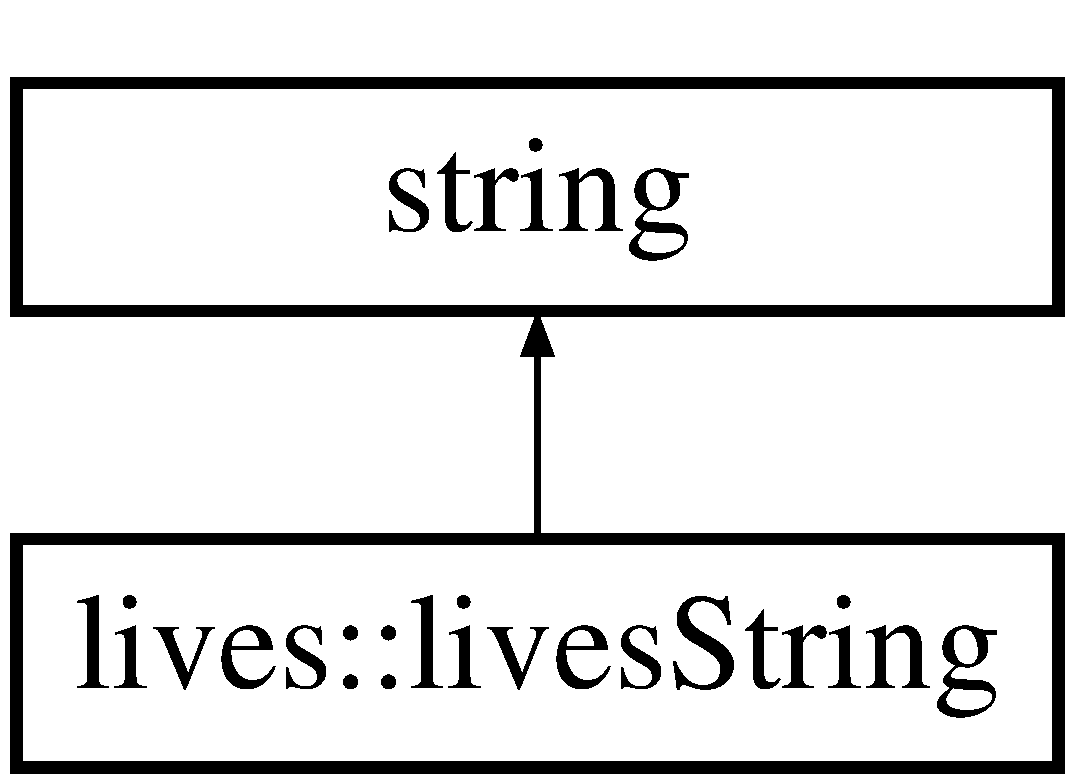
\includegraphics[height=2.000000cm]{classlives_1_1livesString}
\end{center}
\end{figure}
\subsection*{Public Member Functions}
\begin{DoxyCompactItemize}
\item 
\hypertarget{classlives_1_1livesString_a6819728f52f9a669f71e7dc0a806d0cb}{{\bfseries lives\-String} (const string \&str=\char`\"{}\char`\"{}, \hyperlink{liblives_8hpp_ac7022da9e6d00c731395516feb5dc3e5}{lives\-\_\-char\-\_\-encoding\-\_\-t} e=\hyperlink{liblives_8hpp_aa725ee775f37908fca65f712c202b6c9}{L\-I\-V\-E\-S\-\_\-\-C\-H\-A\-R\-\_\-\-E\-N\-C\-O\-D\-I\-N\-G\-\_\-\-D\-E\-F\-A\-U\-L\-T})}\label{classlives_1_1livesString_a6819728f52f9a669f71e7dc0a806d0cb}

\item 
\hypertarget{classlives_1_1livesString_af81e94452b36a08fc23afb01c0a69aa1}{{\bfseries lives\-String} (const string \&str, size\-\_\-t pos, size\-\_\-t len=npos, \hyperlink{liblives_8hpp_ac7022da9e6d00c731395516feb5dc3e5}{lives\-\_\-char\-\_\-encoding\-\_\-t} e=\hyperlink{liblives_8hpp_aa725ee775f37908fca65f712c202b6c9}{L\-I\-V\-E\-S\-\_\-\-C\-H\-A\-R\-\_\-\-E\-N\-C\-O\-D\-I\-N\-G\-\_\-\-D\-E\-F\-A\-U\-L\-T})}\label{classlives_1_1livesString_af81e94452b36a08fc23afb01c0a69aa1}

\item 
\hypertarget{classlives_1_1livesString_a554abf8380ce3a40b094ab4ee661e7e2}{{\bfseries lives\-String} (const char $\ast$s, \hyperlink{liblives_8hpp_ac7022da9e6d00c731395516feb5dc3e5}{lives\-\_\-char\-\_\-encoding\-\_\-t} e=\hyperlink{liblives_8hpp_aa725ee775f37908fca65f712c202b6c9}{L\-I\-V\-E\-S\-\_\-\-C\-H\-A\-R\-\_\-\-E\-N\-C\-O\-D\-I\-N\-G\-\_\-\-D\-E\-F\-A\-U\-L\-T})}\label{classlives_1_1livesString_a554abf8380ce3a40b094ab4ee661e7e2}

\item 
\hypertarget{classlives_1_1livesString_a05c4d8d63066c7fdf5c5b5e2a80bfeb3}{{\bfseries lives\-String} (const char $\ast$s, size\-\_\-t n, \hyperlink{liblives_8hpp_ac7022da9e6d00c731395516feb5dc3e5}{lives\-\_\-char\-\_\-encoding\-\_\-t} e=\hyperlink{liblives_8hpp_aa725ee775f37908fca65f712c202b6c9}{L\-I\-V\-E\-S\-\_\-\-C\-H\-A\-R\-\_\-\-E\-N\-C\-O\-D\-I\-N\-G\-\_\-\-D\-E\-F\-A\-U\-L\-T})}\label{classlives_1_1livesString_a05c4d8d63066c7fdf5c5b5e2a80bfeb3}

\item 
\hypertarget{classlives_1_1livesString_a6b98bde4fcbac6544f004d9b9ec72ed5}{{\bfseries lives\-String} (size\-\_\-t n, char c, \hyperlink{liblives_8hpp_ac7022da9e6d00c731395516feb5dc3e5}{lives\-\_\-char\-\_\-encoding\-\_\-t} e=\hyperlink{liblives_8hpp_aa725ee775f37908fca65f712c202b6c9}{L\-I\-V\-E\-S\-\_\-\-C\-H\-A\-R\-\_\-\-E\-N\-C\-O\-D\-I\-N\-G\-\_\-\-D\-E\-F\-A\-U\-L\-T})}\label{classlives_1_1livesString_a6b98bde4fcbac6544f004d9b9ec72ed5}

\item 
\hypertarget{classlives_1_1livesString_a60c109df1843d607dcfc706acaf06106}{{\footnotesize template$<$class Input\-Iterator $>$ }\\{\bfseries lives\-String} (Input\-Iterator first, Input\-Iterator last, \hyperlink{liblives_8hpp_ac7022da9e6d00c731395516feb5dc3e5}{lives\-\_\-char\-\_\-encoding\-\_\-t} e=\hyperlink{liblives_8hpp_aa725ee775f37908fca65f712c202b6c9}{L\-I\-V\-E\-S\-\_\-\-C\-H\-A\-R\-\_\-\-E\-N\-C\-O\-D\-I\-N\-G\-\_\-\-D\-E\-F\-A\-U\-L\-T})}\label{classlives_1_1livesString_a60c109df1843d607dcfc706acaf06106}

\item 
\hyperlink{classlives_1_1livesString}{lives\-String} \hyperlink{classlives_1_1livesString_a26e5c709b1ccc19f09997e70dbd64284}{to\-Encoding} (\hyperlink{liblives_8hpp_ac7022da9e6d00c731395516feb5dc3e5}{lives\-\_\-char\-\_\-encoding\-\_\-t} enc)
\begin{DoxyCompactList}\small\item\em Change the character encoding of the string. \end{DoxyCompactList}\item 
void \hyperlink{classlives_1_1livesString_a8dc089efbebeb250a2427722447626a9}{set\-Encoding} (\hyperlink{liblives_8hpp_ac7022da9e6d00c731395516feb5dc3e5}{lives\-\_\-char\-\_\-encoding\-\_\-t} enc)
\begin{DoxyCompactList}\small\item\em Define the character encoding of the string. \end{DoxyCompactList}\item 
\hyperlink{liblives_8hpp_ac7022da9e6d00c731395516feb5dc3e5}{lives\-\_\-char\-\_\-encoding\-\_\-t} \hyperlink{classlives_1_1livesString_ae4b4cdac9f59eb13697b42bf9d97cdfa}{encoding} ()
\begin{DoxyCompactList}\small\item\em Return the encoding that the string was declared as. \end{DoxyCompactList}\end{DoxyCompactItemize}


\subsection{Detailed Description}
class \char`\"{}lives\-String\char`\"{}. 

A subclass of std\-::string which automatically handles various character encodings. 

\subsection{Member Function Documentation}
\hypertarget{classlives_1_1livesString_ae4b4cdac9f59eb13697b42bf9d97cdfa}{\index{lives\-::lives\-String@{lives\-::lives\-String}!encoding@{encoding}}
\index{encoding@{encoding}!lives::livesString@{lives\-::lives\-String}}
\subsubsection[{encoding}]{\setlength{\rightskip}{0pt plus 5cm}{\bf lives\-\_\-char\-\_\-encoding\-\_\-t} lives\-::lives\-String\-::encoding (
\begin{DoxyParamCaption}
{}
\end{DoxyParamCaption}
)}}\label{classlives_1_1livesString_ae4b4cdac9f59eb13697b42bf9d97cdfa}


Return the encoding that the string was declared as. 

\begin{DoxyReturn}{Returns}
the character encoding the string is in. 
\end{DoxyReturn}
\hypertarget{classlives_1_1livesString_a8dc089efbebeb250a2427722447626a9}{\index{lives\-::lives\-String@{lives\-::lives\-String}!set\-Encoding@{set\-Encoding}}
\index{set\-Encoding@{set\-Encoding}!lives::livesString@{lives\-::lives\-String}}
\subsubsection[{set\-Encoding}]{\setlength{\rightskip}{0pt plus 5cm}void lives\-::lives\-String\-::set\-Encoding (
\begin{DoxyParamCaption}
\item[{{\bf lives\-\_\-char\-\_\-encoding\-\_\-t}}]{enc}
\end{DoxyParamCaption}
)}}\label{classlives_1_1livesString_a8dc089efbebeb250a2427722447626a9}


Define the character encoding of the string. 


\begin{DoxyParams}{Parameters}
{\em enc} & the character encoding the string is in. \\
\hline
\end{DoxyParams}
\hypertarget{classlives_1_1livesString_a26e5c709b1ccc19f09997e70dbd64284}{\index{lives\-::lives\-String@{lives\-::lives\-String}!to\-Encoding@{to\-Encoding}}
\index{to\-Encoding@{to\-Encoding}!lives::livesString@{lives\-::lives\-String}}
\subsubsection[{to\-Encoding}]{\setlength{\rightskip}{0pt plus 5cm}{\bf lives\-String} lives\-::lives\-String\-::to\-Encoding (
\begin{DoxyParamCaption}
\item[{{\bf lives\-\_\-char\-\_\-encoding\-\_\-t}}]{enc}
\end{DoxyParamCaption}
)}}\label{classlives_1_1livesString_a26e5c709b1ccc19f09997e70dbd64284}


Change the character encoding of the string. 


\begin{DoxyParams}{Parameters}
{\em enc} & the character encoding to convert to. \\
\hline
\end{DoxyParams}
\begin{DoxyReturn}{Returns}
either the same string if no conversion is needed, or a new string if conversion is needed 
\end{DoxyReturn}


The documentation for this class was generated from the following files\-:\begin{DoxyCompactItemize}
\item 
src/\hyperlink{liblives_8hpp}{liblives.\-hpp}\item 
src/\hyperlink{liblives_8cpp}{liblives.\-cpp}\end{DoxyCompactItemize}

\hypertarget{structlives_1_1modeChangedInfo}{\section{lives\-:\-:mode\-Changed\-Info Struct Reference}
\label{structlives_1_1modeChangedInfo}\index{lives\-::mode\-Changed\-Info@{lives\-::mode\-Changed\-Info}}
}


Struct passed to mode\-Changed callback.  




{\ttfamily \#include $<$liblives.\-hpp$>$}

\subsection*{Public Attributes}
\begin{DoxyCompactItemize}
\item 
\hypertarget{structlives_1_1modeChangedInfo_abc4dd856262f42b9c121c53d2895d6a8}{\hyperlink{liblives_8hpp_a3033beb0f401e14cbff66f72a4168d1f}{lives\-\_\-interface\-\_\-mode\-\_\-t} \hyperlink{structlives_1_1modeChangedInfo_abc4dd856262f42b9c121c53d2895d6a8}{mode}}\label{structlives_1_1modeChangedInfo_abc4dd856262f42b9c121c53d2895d6a8}

\begin{DoxyCompactList}\small\item\em mode changed to \end{DoxyCompactList}\end{DoxyCompactItemize}


\subsection{Detailed Description}
Struct passed to mode\-Changed callback. 

The documentation for this struct was generated from the following file\-:\begin{DoxyCompactItemize}
\item 
src/\hyperlink{liblives_8hpp}{liblives.\-hpp}\end{DoxyCompactItemize}

\hypertarget{classlives_1_1multitrack}{\section{lives\-:\-:multitrack Class Reference}
\label{classlives_1_1multitrack}\index{lives\-::multitrack@{lives\-::multitrack}}
}


class \char`\"{}multitrack\char`\"{}.  




{\ttfamily \#include $<$liblives.\-hpp$>$}

\subsection*{Public Member Functions}
\begin{DoxyCompactItemize}
\item 
bool \hyperlink{classlives_1_1multitrack_ab3cfc5e22b91d440a6042edf89128443}{is\-Valid} () const 
\begin{DoxyCompactList}\small\item\em returns whether the multitrack is valid or not. \end{DoxyCompactList}\item 
bool \hyperlink{classlives_1_1multitrack_adeb7b705e8e050f64673e938dddf2e36}{is\-Active} () const 
\begin{DoxyCompactList}\small\item\em returns whether the multitrack is active or not. \end{DoxyCompactList}\item 
bool \hyperlink{classlives_1_1multitrack_a5c460e735627c14a0ed9c7762ec16605}{set\-Current\-Track} (int track) const 
\begin{DoxyCompactList}\small\item\em Set the current track if \hyperlink{classlives_1_1multitrack_adeb7b705e8e050f64673e938dddf2e36}{is\-Active()} is true. \end{DoxyCompactList}\item 
int \hyperlink{classlives_1_1multitrack_afd651f56d20b98bf46d68ccfa25c50e8}{current\-Track} () const 
\begin{DoxyCompactList}\small\item\em If \hyperlink{classlives_1_1multitrack_adeb7b705e8e050f64673e938dddf2e36}{is\-Active()} is true, then this method returns the current active track. \end{DoxyCompactList}\item 
double \hyperlink{classlives_1_1multitrack_ad793b13bd2843823b594e43e0e058a52}{set\-Current\-Time} (double time) const 
\begin{DoxyCompactList}\small\item\em Set the current playback start time in seconds. \end{DoxyCompactList}\item 
double \hyperlink{classlives_1_1multitrack_a30f00aaa45426e7035cab06878481ccb}{current\-Time} () const 
\begin{DoxyCompactList}\small\item\em Return the current playback time in seconds. \end{DoxyCompactList}\item 
\hyperlink{classlives_1_1livesString}{lives\-String} \hyperlink{classlives_1_1multitrack_acae4482fa4581f46fec031459c1c82e5}{track\-Label} (int track) const 
\begin{DoxyCompactList}\small\item\em If \hyperlink{classlives_1_1multitrack_adeb7b705e8e050f64673e938dddf2e36}{is\-Active()} is true, then this method returns the label for a track. \end{DoxyCompactList}\item 
bool \hyperlink{classlives_1_1multitrack_a50d2874d3db625d3cc2ea50f2d0e6e87}{set\-Track\-Label} (int track, \hyperlink{classlives_1_1livesString}{lives\-String} label=\hyperlink{classlives_1_1livesString}{lives\-String}()) const 
\begin{DoxyCompactList}\small\item\em Set the label for a track. \end{DoxyCompactList}\item 
\hyperlink{liblives_8hpp_a85e44abde9be7196c1da9fd5922b7558}{lives\-\_\-gravity\-\_\-t} \hyperlink{classlives_1_1multitrack_a9bf9b673e0a9b38e9e9c6e08d93ce9e7}{gravity} () const 
\begin{DoxyCompactList}\small\item\em Returns the value of the multitrack gravity. \end{DoxyCompactList}\item 
\hyperlink{liblives_8hpp_a85e44abde9be7196c1da9fd5922b7558}{lives\-\_\-gravity\-\_\-t} \hyperlink{classlives_1_1multitrack_a7b2751e2cdafd83bb61956d3ef8dbf75}{set\-Gravity} (\hyperlink{liblives_8hpp_a85e44abde9be7196c1da9fd5922b7558}{lives\-\_\-gravity\-\_\-t}) const 
\begin{DoxyCompactList}\small\item\em Set the gravity mode for multitrack. \end{DoxyCompactList}\item 
\hyperlink{liblives_8hpp_a38030320722a0ce9eabf23a05e313ac5}{lives\-\_\-insert\-\_\-mode\-\_\-t} \hyperlink{classlives_1_1multitrack_af8aee088d4a3cab50e6d2565af599356}{insert\-Mode} () const 
\begin{DoxyCompactList}\small\item\em Returns the value of the multitrack insert mode. \end{DoxyCompactList}\item 
\hyperlink{liblives_8hpp_a38030320722a0ce9eabf23a05e313ac5}{lives\-\_\-insert\-\_\-mode\-\_\-t} \hyperlink{classlives_1_1multitrack_a7441bc16cee7181e2ca0f428707f0f83}{set\-Insert\-Mode} (\hyperlink{liblives_8hpp_a38030320722a0ce9eabf23a05e313ac5}{lives\-\_\-insert\-\_\-mode\-\_\-t}) const 
\begin{DoxyCompactList}\small\item\em Set the gravity mode for multitrack. \end{DoxyCompactList}\item 
int \hyperlink{classlives_1_1multitrack_a13509e7731f57c25b935cd4a03b49c05}{add\-Video\-Track} (bool in\-\_\-front) const 
\begin{DoxyCompactList}\small\item\em Append a new video track into the timeline. \end{DoxyCompactList}\item 
int \hyperlink{classlives_1_1multitrack_a98ed8d2f9eee0456283908f472facbc3}{num\-Video\-Tracks} () const 
\begin{DoxyCompactList}\small\item\em Returns the number of video tracks for multitrack. \end{DoxyCompactList}\item 
int \hyperlink{classlives_1_1multitrack_a49e84f7e6d8c162afd8f60f8075e2c1a}{num\-Audio\-Tracks} () const 
\begin{DoxyCompactList}\small\item\em Returns the number of audio backing tracks for multitrack. \end{DoxyCompactList}\item 
double \hyperlink{classlives_1_1multitrack_aa5709b2f8bc04c5e3ff14919f2e477f0}{F\-P\-S} () const 
\begin{DoxyCompactList}\small\item\em Return the framerate of the multitrack in frames per second. \end{DoxyCompactList}\item 
\hyperlink{classlives_1_1block}{block} \hyperlink{classlives_1_1multitrack_a2c59268f0edecd2597d48ac997319225}{insert\-Block} (\hyperlink{classlives_1_1clip}{clip} c, bool ignore\-\_\-selection\-\_\-limits=false, bool without\-\_\-audio=false) const 
\begin{DoxyCompactList}\small\item\em Insert frames from clip c into \hyperlink{classlives_1_1multitrack_afd651f56d20b98bf46d68ccfa25c50e8}{current\-Track()} at \hyperlink{classlives_1_1multitrack_a30f00aaa45426e7035cab06878481ccb}{current\-Time()} If ignore\-\_\-selection\-\_\-limits is true, then all frames from the clip will be inserted, otherwise (the default) only frames from \hyperlink{classlives_1_1clip_ae3bec5d06c36693307baab2f0ae2c591}{clip\-::selection\-Start()} to \hyperlink{classlives_1_1clip_a4e2b3c1a80795906f39f27390b8545ae}{clip\-::selection\-End()} will be used. \end{DoxyCompactList}\item 
\hyperlink{classlives_1_1livesString}{lives\-String} \hyperlink{classlives_1_1multitrack_ad885f138aa6c679aa12012c1b8c17eff}{wipe\-Layout} (bool force=false) const 
\begin{DoxyCompactList}\small\item\em Wipe the current layout, leaving a blank layout. \end{DoxyCompactList}\item 
\hyperlink{classlives_1_1livesString}{lives\-String} \hyperlink{classlives_1_1multitrack_a0cca1e969b0a453dd45a22cba913bcd4}{choose\-Layout} () const 
\begin{DoxyCompactList}\small\item\em Allow the user to graphically choose a layout to load for the set. \end{DoxyCompactList}\item 
lives\-String\-List \hyperlink{classlives_1_1multitrack_aa2211ef787da9b6e015489bfe1aaa6ef}{available\-Layouts} () const 
\begin{DoxyCompactList}\small\item\em Return a list of the available layouts for the currently loaded set. \end{DoxyCompactList}\item 
bool \hyperlink{classlives_1_1multitrack_a7b3e2b981aecdd9a76957cb48d2ec7e1}{reload\-Layout} (\hyperlink{classlives_1_1livesString}{lives\-String} filename) const 
\begin{DoxyCompactList}\small\item\em Reload the selected layout, replacing the current multitrack layout. \end{DoxyCompactList}\item 
\hyperlink{classlives_1_1livesString}{lives\-String} \hyperlink{classlives_1_1multitrack_a1317da7f96369c0c9dd31cac1096eaa7}{save\-Layout} (\hyperlink{classlives_1_1livesString}{lives\-String} name) const 
\begin{DoxyCompactList}\small\item\em Save the current layout using the name supplied. \end{DoxyCompactList}\item 
\hyperlink{classlives_1_1livesString}{lives\-String} \hyperlink{classlives_1_1multitrack_a051845885961bd42d7d5f36444b29053}{save\-Layout} () const 
\begin{DoxyCompactList}\small\item\em Save the current layout using the current layout name. \end{DoxyCompactList}\item 
\hyperlink{classlives_1_1clip}{clip} \hyperlink{classlives_1_1multitrack_aa766afca893af628a4e0ed93cd1a211f}{render} (bool render\-\_\-audio=true, bool normalise\-\_\-audio=true) const 
\begin{DoxyCompactList}\small\item\em Render the current layout to a new clip and return it. \end{DoxyCompactList}\item 
\hyperlink{classlives_1_1effect}{effect} \hyperlink{classlives_1_1multitrack_acc79b336b1fe1d2beffce4260b44da4f}{auto\-Transition} () const 
\begin{DoxyCompactList}\small\item\em Returns the current autotransition effect for multitrack mode. \end{DoxyCompactList}\item 
bool \hyperlink{classlives_1_1multitrack_af906b5636a475439947272e83bde0ead}{disable\-Auto\-Transition} () const 
\begin{DoxyCompactList}\small\item\em Set the current autotransition effect for multitrack mode to \char`\"{}\-None\char`\"{} (no effect). \end{DoxyCompactList}\item 
bool \hyperlink{classlives_1_1multitrack_a217f391d49113830176a3f664e2562b7}{set\-Auto\-Transition} (\hyperlink{classlives_1_1effect}{effect} autotrans) const 
\begin{DoxyCompactList}\small\item\em Set the current autotransition effect for multitrack mode. \end{DoxyCompactList}\item 
bool \hyperlink{classlives_1_1multitrack_a29420bc94d63fe785c48b841236c7b51}{operator==} (const \hyperlink{classlives_1_1multitrack}{multitrack} \&other) const 
\end{DoxyCompactItemize}
\subsection*{Protected Member Functions}
\begin{DoxyCompactItemize}
\item 
\hypertarget{classlives_1_1multitrack_a508d9d16c2101dde4e4f7102e82793ac}{\hyperlink{classlives_1_1multitrack_a508d9d16c2101dde4e4f7102e82793ac}{multitrack} (\hyperlink{classlives_1_1livesApp}{lives\-App} $\ast$lives=N\-U\-L\-L)}\label{classlives_1_1multitrack_a508d9d16c2101dde4e4f7102e82793ac}

\begin{DoxyCompactList}\small\item\em multitrack \end{DoxyCompactList}\end{DoxyCompactItemize}
\subsection*{Protected Attributes}
\begin{DoxyCompactItemize}
\item 
\hypertarget{classlives_1_1multitrack_a590315201973b2511750931ae8a5f304}{\hyperlink{classlives_1_1livesApp}{lives\-App} $\ast$ {\bfseries m\-\_\-lives}}\label{classlives_1_1multitrack_a590315201973b2511750931ae8a5f304}

\end{DoxyCompactItemize}


\subsection{Detailed Description}
class \char`\"{}multitrack\char`\"{}. 

Represents the multitrack object in a \hyperlink{classlives_1_1livesApp}{lives\-App}. 

\subsection{Member Function Documentation}
\hypertarget{classlives_1_1multitrack_a13509e7731f57c25b935cd4a03b49c05}{\index{lives\-::multitrack@{lives\-::multitrack}!add\-Video\-Track@{add\-Video\-Track}}
\index{add\-Video\-Track@{add\-Video\-Track}!lives::multitrack@{lives\-::multitrack}}
\subsubsection[{add\-Video\-Track}]{\setlength{\rightskip}{0pt plus 5cm}int lives\-::multitrack\-::add\-Video\-Track (
\begin{DoxyParamCaption}
\item[{bool}]{in\-\_\-front}
\end{DoxyParamCaption}
) const}}\label{classlives_1_1multitrack_a13509e7731f57c25b935cd4a03b49c05}


Append a new video track into the timeline. 

Only works if \hyperlink{classlives_1_1multitrack_adeb7b705e8e050f64673e938dddf2e36}{is\-Active()} is true, and \hyperlink{classlives_1_1livesApp_afcb05464af9146f5efbb896f2611c8e7}{lives\-App\-::status()} is L\-I\-V\-E\-S\-\_\-\-S\-T\-A\-T\-U\-S\-\_\-\-R\-E\-A\-D\-Y. 
\begin{DoxyParams}{Parameters}
{\em in\-\_\-front} & set to true to insert a video track in front of existing video tracks. Otherwise insert will be behind. \\
\hline
\end{DoxyParams}
\begin{DoxyReturn}{Returns}
the index number of the newly added track, or -\/1 if the operation failed. 
\end{DoxyReturn}
\hypertarget{classlives_1_1multitrack_acc79b336b1fe1d2beffce4260b44da4f}{\index{lives\-::multitrack@{lives\-::multitrack}!auto\-Transition@{auto\-Transition}}
\index{auto\-Transition@{auto\-Transition}!lives::multitrack@{lives\-::multitrack}}
\subsubsection[{auto\-Transition}]{\setlength{\rightskip}{0pt plus 5cm}{\bf effect} lives\-::multitrack\-::auto\-Transition (
\begin{DoxyParamCaption}
{}
\end{DoxyParamCaption}
) const}}\label{classlives_1_1multitrack_acc79b336b1fe1d2beffce4260b44da4f}


Returns the current autotransition effect for multitrack mode. 

If no effect is set, returns an invalid effect. If the owning lives\-App\-::is\-Invalid() is true, or if lives\-App\-::\-Status() is L\-I\-V\-E\-S\-\_\-\-S\-T\-A\-T\-U\-S\-\_\-\-N\-O\-T\-R\-E\-A\-D\-Y, returns an invalid effect. \begin{DoxyReturn}{Returns}
the autotransition effect for multitrack. 
\end{DoxyReturn}
\begin{DoxySeeAlso}{See Also}
\hyperlink{classlives_1_1multitrack_a217f391d49113830176a3f664e2562b7}{set\-Auto\-Transition()}. 

\hyperlink{classlives_1_1multitrack_af906b5636a475439947272e83bde0ead}{disable\-Auto\-Transition()}. 
\end{DoxySeeAlso}
\hypertarget{classlives_1_1multitrack_aa2211ef787da9b6e015489bfe1aaa6ef}{\index{lives\-::multitrack@{lives\-::multitrack}!available\-Layouts@{available\-Layouts}}
\index{available\-Layouts@{available\-Layouts}!lives::multitrack@{lives\-::multitrack}}
\subsubsection[{available\-Layouts}]{\setlength{\rightskip}{0pt plus 5cm}lives\-String\-List lives\-::multitrack\-::available\-Layouts (
\begin{DoxyParamCaption}
{}
\end{DoxyParamCaption}
) const}}\label{classlives_1_1multitrack_aa2211ef787da9b6e015489bfe1aaa6ef}


Return a list of the available layouts for the currently loaded set. 

If \hyperlink{classlives_1_1livesApp_a4fcefcf7c5dc1e745a12c5a0c07fe220}{lives\-App\-::is\-Ready()} is false, or if no set is loaded, then an empty lives\-String\-List is returned. \begin{DoxyReturn}{Returns}
list of available layouts for the currently loaded set 
\end{DoxyReturn}
\begin{DoxySeeAlso}{See Also}
\hyperlink{classlives_1_1multitrack_a7b3e2b981aecdd9a76957cb48d2ec7e1}{reload\-Layout()}. 
\end{DoxySeeAlso}
\hypertarget{classlives_1_1multitrack_a0cca1e969b0a453dd45a22cba913bcd4}{\index{lives\-::multitrack@{lives\-::multitrack}!choose\-Layout@{choose\-Layout}}
\index{choose\-Layout@{choose\-Layout}!lives::multitrack@{lives\-::multitrack}}
\subsubsection[{choose\-Layout}]{\setlength{\rightskip}{0pt plus 5cm}{\bf lives\-String} lives\-::multitrack\-::choose\-Layout (
\begin{DoxyParamCaption}
{}
\end{DoxyParamCaption}
) const}}\label{classlives_1_1multitrack_a0cca1e969b0a453dd45a22cba913bcd4}


Allow the user to graphically choose a layout to load for the set. 

Only works if \hyperlink{classlives_1_1livesApp_afcb05464af9146f5efbb896f2611c8e7}{lives\-App\-::status()} is L\-I\-V\-E\-S\-\_\-\-S\-T\-A\-T\-U\-S\-\_\-\-R\-E\-A\-D\-Y and \hyperlink{classlives_1_1multitrack_adeb7b705e8e050f64673e938dddf2e36}{is\-Active()} is true, otherwise an empty \hyperlink{classlives_1_1livesString}{lives\-String} is returned. \begin{DoxyReturn}{Returns}
the name of the layout selected. 
\end{DoxyReturn}
\begin{DoxySeeAlso}{See Also}
\hyperlink{classlives_1_1multitrack_a7b3e2b981aecdd9a76957cb48d2ec7e1}{reload\-Layout()}. 

\hyperlink{classlives_1_1multitrack_aa2211ef787da9b6e015489bfe1aaa6ef}{available\-Layouts()}. 
\end{DoxySeeAlso}
\hypertarget{classlives_1_1multitrack_a30f00aaa45426e7035cab06878481ccb}{\index{lives\-::multitrack@{lives\-::multitrack}!current\-Time@{current\-Time}}
\index{current\-Time@{current\-Time}!lives::multitrack@{lives\-::multitrack}}
\subsubsection[{current\-Time}]{\setlength{\rightskip}{0pt plus 5cm}double lives\-::multitrack\-::current\-Time (
\begin{DoxyParamCaption}
{}
\end{DoxyParamCaption}
) const}}\label{classlives_1_1multitrack_a30f00aaa45426e7035cab06878481ccb}


Return the current playback time in seconds. 

If \hyperlink{classlives_1_1multitrack_adeb7b705e8e050f64673e938dddf2e36}{is\-Active()} is true this returns the current player time in the multitrack timeline (equivalent to to player\-::playback\-Time(), and during playback, equivalent to \hyperlink{classlives_1_1player_a412c342ef5220bafba0c479e9ef9111f}{player\-::elapsed\-Time()} plus a constant offset). This function works when \hyperlink{classlives_1_1livesApp_afcb05464af9146f5efbb896f2611c8e7}{lives\-App\-::status()} is L\-I\-V\-E\-\_\-\-S\-T\-A\-T\-U\-S\-\_\-\-R\-E\-A\-D\-Y or L\-I\-V\-E\-S\-\_\-\-S\-T\-A\-T\-U\-S\-\_\-\-P\-L\-A\-Y\-I\-N\-G. If \hyperlink{classlives_1_1multitrack_adeb7b705e8e050f64673e938dddf2e36}{is\-Active()} is false, 0. is returned. \begin{DoxyReturn}{Returns}
the current clip playback time. 
\end{DoxyReturn}
\begin{DoxySeeAlso}{See Also}
\hyperlink{classlives_1_1multitrack_ad793b13bd2843823b594e43e0e058a52}{set\-Current\-Time()}. 

current\-Audio\-Time(). 

elapsed\-Time(). 
\end{DoxySeeAlso}
\hypertarget{classlives_1_1multitrack_afd651f56d20b98bf46d68ccfa25c50e8}{\index{lives\-::multitrack@{lives\-::multitrack}!current\-Track@{current\-Track}}
\index{current\-Track@{current\-Track}!lives::multitrack@{lives\-::multitrack}}
\subsubsection[{current\-Track}]{\setlength{\rightskip}{0pt plus 5cm}int lives\-::multitrack\-::current\-Track (
\begin{DoxyParamCaption}
{}
\end{DoxyParamCaption}
) const}}\label{classlives_1_1multitrack_afd651f56d20b98bf46d68ccfa25c50e8}


If \hyperlink{classlives_1_1multitrack_adeb7b705e8e050f64673e938dddf2e36}{is\-Active()} is true, then this method returns the current active track. 

The active track defines the insertion point for video and audio, along with the \hyperlink{classlives_1_1multitrack_a30f00aaa45426e7035cab06878481ccb}{current\-Time()}. If \hyperlink{classlives_1_1multitrack_adeb7b705e8e050f64673e938dddf2e36}{is\-Active()} is false, or the \hyperlink{classlives_1_1livesApp_afcb05464af9146f5efbb896f2611c8e7}{lives\-App\-::status} is not L\-I\-V\-E\-S\-\_\-\-S\-T\-A\-T\-U\-S\-\_\-\-R\-E\-A\-D\-Y or L\-I\-V\-E\-S\-\_\-\-S\-T\-A\-T\-U\-S\-\_\-\-P\-L\-A\-Y\-I\-N\-G then the return value is undefined. \begin{DoxyReturn}{Returns}
the current active track in multitrack mode. A value $>$= 0 represents a video track, a value $<$ 0 represents a backing audio track. 
\end{DoxyReturn}
\begin{DoxySeeAlso}{See Also}
\hyperlink{classlives_1_1multitrack_a5c460e735627c14a0ed9c7762ec16605}{set\-Current\-Track()}. 
\end{DoxySeeAlso}
\hypertarget{classlives_1_1multitrack_af906b5636a475439947272e83bde0ead}{\index{lives\-::multitrack@{lives\-::multitrack}!disable\-Auto\-Transition@{disable\-Auto\-Transition}}
\index{disable\-Auto\-Transition@{disable\-Auto\-Transition}!lives::multitrack@{lives\-::multitrack}}
\subsubsection[{disable\-Auto\-Transition}]{\setlength{\rightskip}{0pt plus 5cm}bool lives\-::multitrack\-::disable\-Auto\-Transition (
\begin{DoxyParamCaption}
{}
\end{DoxyParamCaption}
) const}}\label{classlives_1_1multitrack_af906b5636a475439947272e83bde0ead}


Set the current autotransition effect for multitrack mode to \char`\"{}\-None\char`\"{} (no effect). 

If the \hyperlink{classlives_1_1livesApp_afcb05464af9146f5efbb896f2611c8e7}{lives\-App\-::status()} is not L\-I\-V\-E\-S\-\_\-\-S\-T\-A\-T\-U\-S\-\_\-\-R\-E\-A\-D\-Y or L\-I\-V\-E\-S\-\_\-\-S\-T\-A\-T\-U\-S\-\_\-\-P\-L\-A\-Y\-I\-N\-G, returns false and nothing happens. \begin{DoxyReturn}{Returns}
true if the autotransition was disabled. 
\end{DoxyReturn}
\begin{DoxySeeAlso}{See Also}
\hyperlink{classlives_1_1multitrack_acc79b336b1fe1d2beffce4260b44da4f}{auto\-Transition()}. 

\hyperlink{classlives_1_1multitrack_a217f391d49113830176a3f664e2562b7}{set\-Auto\-Transition()}. 
\end{DoxySeeAlso}
\hypertarget{classlives_1_1multitrack_aa5709b2f8bc04c5e3ff14919f2e477f0}{\index{lives\-::multitrack@{lives\-::multitrack}!F\-P\-S@{F\-P\-S}}
\index{F\-P\-S@{F\-P\-S}!lives::multitrack@{lives\-::multitrack}}
\subsubsection[{F\-P\-S}]{\setlength{\rightskip}{0pt plus 5cm}double lives\-::multitrack\-::\-F\-P\-S (
\begin{DoxyParamCaption}
{}
\end{DoxyParamCaption}
) const}}\label{classlives_1_1multitrack_aa5709b2f8bc04c5e3ff14919f2e477f0}


Return the framerate of the multitrack in frames per second. 

If \hyperlink{classlives_1_1multitrack_adeb7b705e8e050f64673e938dddf2e36}{is\-Active()} is false, returns 0. Otherwise when the lives\-A\-P\-P\-::status() is L\-I\-V\-E\-S\-\_\-\-S\-T\-A\-T\-U\-S\-\_\-\-P\-L\-A\-Y\-I\-N\-G, player\-::\-F\-P\-S() takes this value. \begin{DoxyReturn}{Returns}
the framerate of the multitrack in frames per second. 
\end{DoxyReturn}
\hypertarget{classlives_1_1multitrack_a9bf9b673e0a9b38e9e9c6e08d93ce9e7}{\index{lives\-::multitrack@{lives\-::multitrack}!gravity@{gravity}}
\index{gravity@{gravity}!lives::multitrack@{lives\-::multitrack}}
\subsubsection[{gravity}]{\setlength{\rightskip}{0pt plus 5cm}{\bf lives\-\_\-gravity\-\_\-t} lives\-::multitrack\-::gravity (
\begin{DoxyParamCaption}
{}
\end{DoxyParamCaption}
) const}}\label{classlives_1_1multitrack_a9bf9b673e0a9b38e9e9c6e08d93ce9e7}


Returns the value of the multitrack gravity. 

This value, together with the \hyperlink{classlives_1_1multitrack_af8aee088d4a3cab50e6d2565af599356}{insert\-Mode()} defines what happens when a block is inserted, moved or deleted. If \hyperlink{classlives_1_1multitrack_adeb7b705e8e050f64673e938dddf2e36}{is\-Active()} is false, the return value is undefined. \begin{DoxyReturn}{Returns}
the multitrack gravity. 
\end{DoxyReturn}
\begin{DoxySeeAlso}{See Also}
\hyperlink{classlives_1_1multitrack_af8aee088d4a3cab50e6d2565af599356}{insert\-Mode()}. 
\end{DoxySeeAlso}
\hypertarget{classlives_1_1multitrack_a2c59268f0edecd2597d48ac997319225}{\index{lives\-::multitrack@{lives\-::multitrack}!insert\-Block@{insert\-Block}}
\index{insert\-Block@{insert\-Block}!lives::multitrack@{lives\-::multitrack}}
\subsubsection[{insert\-Block}]{\setlength{\rightskip}{0pt plus 5cm}{\bf block} lives\-::multitrack\-::insert\-Block (
\begin{DoxyParamCaption}
\item[{{\bf clip}}]{c, }
\item[{bool}]{ignore\-\_\-selection\-\_\-limits = {\ttfamily false}, }
\item[{bool}]{without\-\_\-audio = {\ttfamily false}}
\end{DoxyParamCaption}
) const}}\label{classlives_1_1multitrack_a2c59268f0edecd2597d48ac997319225}


Insert frames from clip c into \hyperlink{classlives_1_1multitrack_afd651f56d20b98bf46d68ccfa25c50e8}{current\-Track()} at \hyperlink{classlives_1_1multitrack_a30f00aaa45426e7035cab06878481ccb}{current\-Time()} If ignore\-\_\-selection\-\_\-limits is true, then all frames from the clip will be inserted, otherwise (the default) only frames from \hyperlink{classlives_1_1clip_ae3bec5d06c36693307baab2f0ae2c591}{clip\-::selection\-Start()} to \hyperlink{classlives_1_1clip_a4e2b3c1a80795906f39f27390b8545ae}{clip\-::selection\-End()} will be used. 

If without\-\_\-audio is false (the default), audio is also inserted. Frames are automatically resampled to fit layout\-::fps(). Depending on the \hyperlink{classlives_1_1multitrack_af8aee088d4a3cab50e6d2565af599356}{insert\-Mode()}, it may not be possible to do the insertion. In case of failure an invalid block is returned. If the current track is a backing audio track, then only audio is inserted; in this case if without\-\_\-audio is true an invalid block is returned. Only works if \hyperlink{classlives_1_1livesApp_afcb05464af9146f5efbb896f2611c8e7}{lives\-App\-::status()} is L\-I\-V\-E\-S\-\_\-\-S\-T\-A\-T\-U\-S\-\_\-\-R\-E\-A\-D\-Y and \hyperlink{classlives_1_1multitrack_adeb7b705e8e050f64673e938dddf2e36}{is\-Active()} is true. Note\-: the actual place where the block ends up, and its final size depends on various factors such as the \hyperlink{classlives_1_1multitrack_a9bf9b673e0a9b38e9e9c6e08d93ce9e7}{gravity()} setting, the \hyperlink{classlives_1_1multitrack_af8aee088d4a3cab50e6d2565af599356}{insert\-Mode()} setting, and the location of other blocks in the layout. The insertion may cause other blocks to relocate. 
\begin{DoxyParams}{Parameters}
{\em c} & the clip to insert from \\
\hline
{\em ignore\-\_\-selection\-\_\-limits} & if true then all frames from the clip will be inserted \\
\hline
{\em without\-\_\-audio} & if false then audio is also inserted \\
\hline
\end{DoxyParams}
\begin{DoxyReturn}{Returns}
the newly inserted block. 
\end{DoxyReturn}
\begin{DoxySeeAlso}{See Also}
\hyperlink{classlives_1_1multitrack_a5c460e735627c14a0ed9c7762ec16605}{set\-Current\-Track()}. 

\hyperlink{classlives_1_1multitrack_ad793b13bd2843823b594e43e0e058a52}{set\-Current\-Time()}. 

\hyperlink{classlives_1_1clip_a01d1d840575c077e8c44ebe71df4ef82}{clip\-::set\-Selection\-Start()}. 

\hyperlink{classlives_1_1clip_abb198e92872582f71ce178e0a0c4c9ac}{clip\-::set\-Selection\-End()}. 

\hyperlink{classlives_1_1multitrack_a7b2751e2cdafd83bb61956d3ef8dbf75}{set\-Gravity()}. 

\hyperlink{classlives_1_1block_a9127196f416f0538a53facf6838021f1}{block\-::remove()}. 
\end{DoxySeeAlso}
\hypertarget{classlives_1_1multitrack_af8aee088d4a3cab50e6d2565af599356}{\index{lives\-::multitrack@{lives\-::multitrack}!insert\-Mode@{insert\-Mode}}
\index{insert\-Mode@{insert\-Mode}!lives::multitrack@{lives\-::multitrack}}
\subsubsection[{insert\-Mode}]{\setlength{\rightskip}{0pt plus 5cm}{\bf lives\-\_\-insert\-\_\-mode\-\_\-t} lives\-::multitrack\-::insert\-Mode (
\begin{DoxyParamCaption}
{}
\end{DoxyParamCaption}
) const}}\label{classlives_1_1multitrack_af8aee088d4a3cab50e6d2565af599356}


Returns the value of the multitrack insert mode. 

This value, together with \hyperlink{classlives_1_1multitrack_a9bf9b673e0a9b38e9e9c6e08d93ce9e7}{gravity()} defines what happens when a block is inserted, moved or deleted. If \hyperlink{classlives_1_1multitrack_adeb7b705e8e050f64673e938dddf2e36}{is\-Active()} is false, the return value is undefined. \begin{DoxyReturn}{Returns}
the multitrack insert mode. 
\end{DoxyReturn}
\begin{DoxySeeAlso}{See Also}
\hyperlink{classlives_1_1multitrack_a9bf9b673e0a9b38e9e9c6e08d93ce9e7}{gravity()}. 
\end{DoxySeeAlso}
\hypertarget{classlives_1_1multitrack_adeb7b705e8e050f64673e938dddf2e36}{\index{lives\-::multitrack@{lives\-::multitrack}!is\-Active@{is\-Active}}
\index{is\-Active@{is\-Active}!lives::multitrack@{lives\-::multitrack}}
\subsubsection[{is\-Active}]{\setlength{\rightskip}{0pt plus 5cm}bool lives\-::multitrack\-::is\-Active (
\begin{DoxyParamCaption}
{}
\end{DoxyParamCaption}
) const}}\label{classlives_1_1multitrack_adeb7b705e8e050f64673e938dddf2e36}


returns whether the multitrack is active or not. 

This is equivent to \hyperlink{classlives_1_1livesApp_aafa7b7f9c2666d097d0413e84bf4eccc}{lives\-App\-::mode()} == L\-I\-V\-E\-S\-\_\-\-I\-N\-T\-E\-R\-F\-A\-C\-E\-\_\-\-M\-O\-D\-E\-\_\-\-M\-U\-L\-T\-I\-T\-R\-A\-C\-K. \begin{DoxyReturn}{Returns}
whether the multitrack is active or not. 
\end{DoxyReturn}
\hypertarget{classlives_1_1multitrack_ab3cfc5e22b91d440a6042edf89128443}{\index{lives\-::multitrack@{lives\-::multitrack}!is\-Valid@{is\-Valid}}
\index{is\-Valid@{is\-Valid}!lives::multitrack@{lives\-::multitrack}}
\subsubsection[{is\-Valid}]{\setlength{\rightskip}{0pt plus 5cm}bool lives\-::multitrack\-::is\-Valid (
\begin{DoxyParamCaption}
{}
\end{DoxyParamCaption}
) const}}\label{classlives_1_1multitrack_ab3cfc5e22b91d440a6042edf89128443}


returns whether the multitrack is valid or not. 

A valid multitrack is one which is owned by a valid \hyperlink{classlives_1_1livesApp}{lives\-App}, whose \hyperlink{classlives_1_1livesApp_afcb05464af9146f5efbb896f2611c8e7}{lives\-App\-::status()} is not L\-I\-V\-E\-S\-\_\-\-S\-T\-A\-T\-U\-S\-\_\-\-N\-O\-T\-R\-E\-A\-D\-Y. \begin{DoxyReturn}{Returns}
whether the multitrack is valid 
\end{DoxyReturn}
\hypertarget{classlives_1_1multitrack_a49e84f7e6d8c162afd8f60f8075e2c1a}{\index{lives\-::multitrack@{lives\-::multitrack}!num\-Audio\-Tracks@{num\-Audio\-Tracks}}
\index{num\-Audio\-Tracks@{num\-Audio\-Tracks}!lives::multitrack@{lives\-::multitrack}}
\subsubsection[{num\-Audio\-Tracks}]{\setlength{\rightskip}{0pt plus 5cm}int lives\-::multitrack\-::num\-Audio\-Tracks (
\begin{DoxyParamCaption}
{}
\end{DoxyParamCaption}
) const}}\label{classlives_1_1multitrack_a49e84f7e6d8c162afd8f60f8075e2c1a}


Returns the number of audio backing tracks for multitrack. 

If \hyperlink{classlives_1_1multitrack_adeb7b705e8e050f64673e938dddf2e36}{is\-Active()} is false, 0 is returned. \begin{DoxyReturn}{Returns}
the number of audio tracks 
\end{DoxyReturn}
\hypertarget{classlives_1_1multitrack_a98ed8d2f9eee0456283908f472facbc3}{\index{lives\-::multitrack@{lives\-::multitrack}!num\-Video\-Tracks@{num\-Video\-Tracks}}
\index{num\-Video\-Tracks@{num\-Video\-Tracks}!lives::multitrack@{lives\-::multitrack}}
\subsubsection[{num\-Video\-Tracks}]{\setlength{\rightskip}{0pt plus 5cm}int lives\-::multitrack\-::num\-Video\-Tracks (
\begin{DoxyParamCaption}
{}
\end{DoxyParamCaption}
) const}}\label{classlives_1_1multitrack_a98ed8d2f9eee0456283908f472facbc3}


Returns the number of video tracks for multitrack. 

If \hyperlink{classlives_1_1multitrack_adeb7b705e8e050f64673e938dddf2e36}{is\-Active()} is false, 0 is returned. \begin{DoxyReturn}{Returns}
the number of video tracks 
\end{DoxyReturn}
\begin{DoxySeeAlso}{See Also}
\hyperlink{classlives_1_1multitrack_a13509e7731f57c25b935cd4a03b49c05}{add\-Video\-Track()} 
\end{DoxySeeAlso}
\hypertarget{classlives_1_1multitrack_a29420bc94d63fe785c48b841236c7b51}{\index{lives\-::multitrack@{lives\-::multitrack}!operator==@{operator==}}
\index{operator==@{operator==}!lives::multitrack@{lives\-::multitrack}}
\subsubsection[{operator==}]{\setlength{\rightskip}{0pt plus 5cm}bool lives\-::multitrack\-::operator== (
\begin{DoxyParamCaption}
\item[{const {\bf multitrack} \&}]{other}
\end{DoxyParamCaption}
) const\hspace{0.3cm}{\ttfamily [inline]}}}\label{classlives_1_1multitrack_a29420bc94d63fe785c48b841236c7b51}
\begin{DoxyReturn}{Returns}
true if the two layouts have the same \hyperlink{classlives_1_1livesApp}{lives\-App} owner 
\end{DoxyReturn}
\hypertarget{classlives_1_1multitrack_a7b3e2b981aecdd9a76957cb48d2ec7e1}{\index{lives\-::multitrack@{lives\-::multitrack}!reload\-Layout@{reload\-Layout}}
\index{reload\-Layout@{reload\-Layout}!lives::multitrack@{lives\-::multitrack}}
\subsubsection[{reload\-Layout}]{\setlength{\rightskip}{0pt plus 5cm}bool lives\-::multitrack\-::reload\-Layout (
\begin{DoxyParamCaption}
\item[{{\bf lives\-String}}]{filename}
\end{DoxyParamCaption}
) const}}\label{classlives_1_1multitrack_a7b3e2b981aecdd9a76957cb48d2ec7e1}


Reload the selected layout, replacing the current multitrack layout. 

Only works if \hyperlink{classlives_1_1livesApp_afcb05464af9146f5efbb896f2611c8e7}{lives\-App\-::status()} is L\-I\-V\-E\-S\-\_\-\-S\-T\-A\-T\-U\-S\-\_\-\-R\-E\-A\-D\-Y and \hyperlink{classlives_1_1multitrack_adeb7b705e8e050f64673e938dddf2e36}{is\-Active()} is true. The layout must be \char`\"{}owned\char`\"{} by the currently loaded set, otherwise an error may be shown and it will not be loaded. If filename is an empty \hyperlink{classlives_1_1livesString}{lives\-String}, \hyperlink{classlives_1_1multitrack_a0cca1e969b0a453dd45a22cba913bcd4}{choose\-Layout()} will be called first to get the layout name. If \hyperlink{classlives_1_1livesApp_a33b85eae23bbb5e55c9843b9016dcff9}{lives\-App\-::interactive()} is true, the user will have a chance to save the current layout (if any) first. 
\begin{DoxyParams}{Parameters}
{\em the} & filename of the layout to load \\
\hline
\end{DoxyParams}
\begin{DoxyReturn}{Returns}
true if the specified layout could be loaded 
\end{DoxyReturn}
\begin{DoxySeeAlso}{See Also}
\hyperlink{classlives_1_1multitrack_a0cca1e969b0a453dd45a22cba913bcd4}{choose\-Layout()}. 

\hyperlink{classlives_1_1multitrack_aa2211ef787da9b6e015489bfe1aaa6ef}{available\-Layouts()}. 

\hyperlink{classlives_1_1multitrack_a1317da7f96369c0c9dd31cac1096eaa7}{save\-Layout()}. 
\end{DoxySeeAlso}
\hypertarget{classlives_1_1multitrack_aa766afca893af628a4e0ed93cd1a211f}{\index{lives\-::multitrack@{lives\-::multitrack}!render@{render}}
\index{render@{render}!lives::multitrack@{lives\-::multitrack}}
\subsubsection[{render}]{\setlength{\rightskip}{0pt plus 5cm}{\bf clip} lives\-::multitrack\-::render (
\begin{DoxyParamCaption}
\item[{bool}]{render\-\_\-audio = {\ttfamily true}, }
\item[{bool}]{normalise\-\_\-audio = {\ttfamily true}}
\end{DoxyParamCaption}
) const}}\label{classlives_1_1multitrack_aa766afca893af628a4e0ed93cd1a211f}


Render the current layout to a new clip and return it. 

Only works if \hyperlink{classlives_1_1multitrack_adeb7b705e8e050f64673e938dddf2e36}{is\-Active()} is true, and \hyperlink{classlives_1_1livesApp_afcb05464af9146f5efbb896f2611c8e7}{lives\-App\-::status()} is L\-I\-V\-E\-S\-\_\-\-S\-T\-A\-T\-U\-S\-\_\-\-R\-E\-A\-D\-Y, and the current layout is not empty. If \hyperlink{classlives_1_1livesApp_a33b85eae23bbb5e55c9843b9016dcff9}{lives\-App\-::interactive()} is true, the user may choose to cancel the operation, or to render fewer than all frames. After rendering, if \hyperlink{namespacelives_1_1prefs_a47055c8f50d9191d66337e53eb447c9f}{prefs\-::mt\-Exit\-Render()} is true, the \hyperlink{classlives_1_1livesApp_aafa7b7f9c2666d097d0413e84bf4eccc}{lives\-App\-::mode()} will change to L\-I\-V\-E\-S\-\_\-\-I\-N\-T\-E\-R\-F\-A\-C\-E\-\_\-\-M\-O\-D\-E\-\_\-\-C\-L\-I\-P\-E\-D\-I\-T, and \hyperlink{classlives_1_1multitrack_adeb7b705e8e050f64673e938dddf2e36}{is\-Active()} will change to false. 
\begin{DoxyParams}{Parameters}
{\em render\-\_\-audio} & true if audio should be rendered in addition to video. \\
\hline
{\em normalise\-\_\-audio} & if true then the audio volume is normalized (backing audio gets half volume, video tracks get half volume) \\
\hline
\end{DoxyParams}
\begin{DoxyReturn}{Returns}
clip a new clip which contains the rendered video, or an invalid clip in case of failure. 
\end{DoxyReturn}
\hypertarget{classlives_1_1multitrack_a1317da7f96369c0c9dd31cac1096eaa7}{\index{lives\-::multitrack@{lives\-::multitrack}!save\-Layout@{save\-Layout}}
\index{save\-Layout@{save\-Layout}!lives::multitrack@{lives\-::multitrack}}
\subsubsection[{save\-Layout}]{\setlength{\rightskip}{0pt plus 5cm}{\bf lives\-String} lives\-::multitrack\-::save\-Layout (
\begin{DoxyParamCaption}
\item[{{\bf lives\-String}}]{name}
\end{DoxyParamCaption}
) const}}\label{classlives_1_1multitrack_a1317da7f96369c0c9dd31cac1096eaa7}


Save the current layout using the name supplied. 

The layout will be saved in the layouts directory for the currently loaded set, so the name should not include any directory component. Only works if the \hyperlink{classlives_1_1livesApp_afcb05464af9146f5efbb896f2611c8e7}{lives\-App\-::status()} is L\-I\-V\-E\-S\-\_\-\-S\-T\-A\-T\-U\-S\-\_\-\-R\-E\-A\-D\-Y, and the current layout is not empty, otherwise an empty \hyperlink{classlives_1_1livesString}{lives\-String} is returned. Note that this W\-I\-L\-L work even if \hyperlink{classlives_1_1multitrack_adeb7b705e8e050f64673e938dddf2e36}{is\-Active()} is false. If \hyperlink{classlives_1_1livesApp_a33b85eae23bbb5e55c9843b9016dcff9}{lives\-App\-::interactive()} is true, the user may choose to cancel the operation. If the layout name is empty, the user will be prompted graphically to enter a name. If the set name is empty, the user will be prompted to enter a set name (if \hyperlink{classlives_1_1livesApp_a33b85eae23bbb5e55c9843b9016dcff9}{lives\-App\-::interactive()} is true; otherwise this will fail and an empty string will be returned). Rarely it will not be possible to save a layout (if it was generated by recording events, and it contains generated audio or video). 
\begin{DoxyParams}{Parameters}
{\em the} & name to save the layout \\
\hline
\end{DoxyParams}
\begin{DoxyReturn}{Returns}
the filename the set was saved to, or empty \hyperlink{classlives_1_1livesString}{lives\-String} if saving failed. 
\end{DoxyReturn}
\begin{DoxySeeAlso}{See Also}
\hyperlink{classlives_1_1multitrack_ad885f138aa6c679aa12012c1b8c17eff}{wipe\-Layout()}. 

\hyperlink{classlives_1_1multitrack_a7b3e2b981aecdd9a76957cb48d2ec7e1}{reload\-Layout()}; 

\hyperlink{classlives_1_1set_a1e41621e140c4770bc502b13b582c6b9}{set\-::set\-Name()}. 
\end{DoxySeeAlso}
\hypertarget{classlives_1_1multitrack_a051845885961bd42d7d5f36444b29053}{\index{lives\-::multitrack@{lives\-::multitrack}!save\-Layout@{save\-Layout}}
\index{save\-Layout@{save\-Layout}!lives::multitrack@{lives\-::multitrack}}
\subsubsection[{save\-Layout}]{\setlength{\rightskip}{0pt plus 5cm}{\bf lives\-String} lives\-::multitrack\-::save\-Layout (
\begin{DoxyParamCaption}
{}
\end{DoxyParamCaption}
) const}}\label{classlives_1_1multitrack_a051845885961bd42d7d5f36444b29053}


Save the current layout using the current layout name. 

Only works if the \hyperlink{classlives_1_1livesApp_afcb05464af9146f5efbb896f2611c8e7}{lives\-App\-::status()} is L\-I\-V\-E\-S\-\_\-\-S\-T\-A\-T\-U\-S\-\_\-\-R\-E\-A\-D\-Y, and the current layout is not empty, otherwise an empty \hyperlink{classlives_1_1livesString}{lives\-String} is returned. Note that this W\-I\-L\-L work even if \hyperlink{classlives_1_1multitrack_adeb7b705e8e050f64673e938dddf2e36}{is\-Active()} is false. If \hyperlink{classlives_1_1livesApp_a33b85eae23bbb5e55c9843b9016dcff9}{lives\-App\-::interactive()} is true, the user may choose to cancel the operation. If the layout name has not been previously set, the user will be prompted graphically to enter a name. If the set name is empty, the user will be prompted to enter a set name (if \hyperlink{classlives_1_1livesApp_a33b85eae23bbb5e55c9843b9016dcff9}{lives\-App\-::interactive()} is true; otherwise this will fail and an empty string will be returned). Rarely it will not be possible to save a layout (if it was generated by recording events, and it contains generated audio or video). 
\begin{DoxyParams}{Parameters}
{\em the} & name to save the layout \\
\hline
\end{DoxyParams}
\begin{DoxyReturn}{Returns}
the filename the set was saved to, or empty \hyperlink{classlives_1_1livesString}{lives\-String} if saving failed. 
\end{DoxyReturn}
\begin{DoxySeeAlso}{See Also}
\hyperlink{classlives_1_1multitrack_ad885f138aa6c679aa12012c1b8c17eff}{wipe\-Layout()}. 

\hyperlink{classlives_1_1multitrack_a7b3e2b981aecdd9a76957cb48d2ec7e1}{reload\-Layout()}; 

\hyperlink{classlives_1_1set_a1e41621e140c4770bc502b13b582c6b9}{set\-::set\-Name()}. 
\end{DoxySeeAlso}
\hypertarget{classlives_1_1multitrack_a217f391d49113830176a3f664e2562b7}{\index{lives\-::multitrack@{lives\-::multitrack}!set\-Auto\-Transition@{set\-Auto\-Transition}}
\index{set\-Auto\-Transition@{set\-Auto\-Transition}!lives::multitrack@{lives\-::multitrack}}
\subsubsection[{set\-Auto\-Transition}]{\setlength{\rightskip}{0pt plus 5cm}bool lives\-::multitrack\-::set\-Auto\-Transition (
\begin{DoxyParamCaption}
\item[{{\bf effect}}]{autotrans}
\end{DoxyParamCaption}
) const}}\label{classlives_1_1multitrack_a217f391d49113830176a3f664e2562b7}


Set the current autotransition effect for multitrack mode. 

If the \hyperlink{classlives_1_1livesApp_afcb05464af9146f5efbb896f2611c8e7}{lives\-App\-::status()} is not L\-I\-V\-E\-S\-\_\-\-S\-T\-A\-T\-U\-S\-\_\-\-R\-E\-A\-D\-Y or L\-I\-V\-E\-S\-\_\-\-S\-T\-A\-T\-U\-S\-\_\-\-P\-L\-A\-Y\-I\-N\-G, returns false and nothing happens. If the effect is not a transition, false is returned and nothing happens. If the effect is invalid, this is the same as calling \hyperlink{classlives_1_1multitrack_af906b5636a475439947272e83bde0ead}{disable\-Auto\-Transition()}. 
\begin{DoxyParams}{Parameters}
{\em the} & new autotransition effect for multitrack. \\
\hline
\end{DoxyParams}
\begin{DoxyReturn}{Returns}
true if the autotransition was changed. 
\end{DoxyReturn}
\begin{DoxySeeAlso}{See Also}
\hyperlink{classlives_1_1multitrack_acc79b336b1fe1d2beffce4260b44da4f}{auto\-Transition()}. 

\hyperlink{classlives_1_1multitrack_af906b5636a475439947272e83bde0ead}{disable\-Auto\-Transition()}. 
\end{DoxySeeAlso}
\hypertarget{classlives_1_1multitrack_ad793b13bd2843823b594e43e0e058a52}{\index{lives\-::multitrack@{lives\-::multitrack}!set\-Current\-Time@{set\-Current\-Time}}
\index{set\-Current\-Time@{set\-Current\-Time}!lives::multitrack@{lives\-::multitrack}}
\subsubsection[{set\-Current\-Time}]{\setlength{\rightskip}{0pt plus 5cm}double lives\-::multitrack\-::set\-Current\-Time (
\begin{DoxyParamCaption}
\item[{double}]{time}
\end{DoxyParamCaption}
) const}}\label{classlives_1_1multitrack_ad793b13bd2843823b594e43e0e058a52}


Set the current playback start time in seconds. 

This is also the insertion point for \hyperlink{classlives_1_1multitrack_a2c59268f0edecd2597d48ac997319225}{insert\-Block()}. Only works if the \hyperlink{classlives_1_1livesApp_afcb05464af9146f5efbb896f2611c8e7}{lives\-App\-::status()} is L\-I\-V\-E\-S\-\_\-\-S\-T\-A\-T\-U\-S\-\_\-\-R\-E\-A\-D\-Y and \hyperlink{classlives_1_1multitrack_adeb7b705e8e050f64673e938dddf2e36}{is\-Active()} is true. Setting the current time may cause the timeline to stretch visually (i.\-e zoom out). The miminum value is 0.\-0; values $<$ 0.\-0 will be ignored. This function is synonymous with player\-::set\-Playback\-Time(). 
\begin{DoxyParams}{Parameters}
{\em time} & the time in seconds to set playback start time to. \\
\hline
\end{DoxyParams}
\begin{DoxyReturn}{Returns}
the new playback start time. 
\end{DoxyReturn}
\begin{DoxySeeAlso}{See Also}
\hyperlink{classlives_1_1multitrack_a30f00aaa45426e7035cab06878481ccb}{current\-Time()}. 
\end{DoxySeeAlso}
\hypertarget{classlives_1_1multitrack_a5c460e735627c14a0ed9c7762ec16605}{\index{lives\-::multitrack@{lives\-::multitrack}!set\-Current\-Track@{set\-Current\-Track}}
\index{set\-Current\-Track@{set\-Current\-Track}!lives::multitrack@{lives\-::multitrack}}
\subsubsection[{set\-Current\-Track}]{\setlength{\rightskip}{0pt plus 5cm}bool lives\-::multitrack\-::set\-Current\-Track (
\begin{DoxyParamCaption}
\item[{int}]{track}
\end{DoxyParamCaption}
) const}}\label{classlives_1_1multitrack_a5c460e735627c14a0ed9c7762ec16605}


Set the current track if \hyperlink{classlives_1_1multitrack_adeb7b705e8e050f64673e938dddf2e36}{is\-Active()} is true. 

Only works when \hyperlink{classlives_1_1livesApp_afcb05464af9146f5efbb896f2611c8e7}{lives\-App\-::status()} is L\-I\-V\-E\-S\-\_\-\-S\-T\-A\-T\-U\-S\-\_\-\-R\-E\-A\-D\-Y or L\-I\-V\-E\-S\-\_\-\-S\-T\-A\-T\-U\-S\-\_\-\-P\-L\-A\-Y\-I\-N\-G. 
\begin{DoxyParams}{Parameters}
{\em track} & a value $>$= 0 represents a video track, a value $<$ 0 represents a backing audio track. \\
\hline
\end{DoxyParams}
\begin{DoxyReturn}{Returns}
true if the track setting was successful. 
\end{DoxyReturn}
\begin{DoxySeeAlso}{See Also}
\hyperlink{classlives_1_1multitrack_afd651f56d20b98bf46d68ccfa25c50e8}{current\-Track()}. 
\end{DoxySeeAlso}
\hypertarget{classlives_1_1multitrack_a7b2751e2cdafd83bb61956d3ef8dbf75}{\index{lives\-::multitrack@{lives\-::multitrack}!set\-Gravity@{set\-Gravity}}
\index{set\-Gravity@{set\-Gravity}!lives::multitrack@{lives\-::multitrack}}
\subsubsection[{set\-Gravity}]{\setlength{\rightskip}{0pt plus 5cm}{\bf lives\-\_\-gravity\-\_\-t} lives\-::multitrack\-::set\-Gravity (
\begin{DoxyParamCaption}
\item[{{\bf lives\-\_\-gravity\-\_\-t}}]{grav}
\end{DoxyParamCaption}
) const}}\label{classlives_1_1multitrack_a7b2751e2cdafd83bb61956d3ef8dbf75}


Set the gravity mode for multitrack. 

If \hyperlink{classlives_1_1multitrack_adeb7b705e8e050f64673e938dddf2e36}{is\-Active()} is false, nothing happens and an undefined value is returned, otherwise if \hyperlink{classlives_1_1livesApp_afcb05464af9146f5efbb896f2611c8e7}{lives\-App\-::status()} is not L\-I\-V\-E\-S\-\_\-\-S\-T\-A\-T\-U\-S\-\_\-\-R\-E\-A\-D\-Y or L\-I\-V\-E\-S\-\_\-\-S\-T\-A\-T\-U\-S\-\_\-\-P\-L\-A\-Y\-I\-N\-G, nothing happens. 
\begin{DoxyParams}{Parameters}
{\em the} & new gravity mode to set. \\
\hline
\end{DoxyParams}
\begin{DoxyReturn}{Returns}
the new gravity mode. 
\end{DoxyReturn}
\begin{DoxySeeAlso}{See Also}
\hyperlink{classlives_1_1multitrack_a9bf9b673e0a9b38e9e9c6e08d93ce9e7}{gravity()}. 
\end{DoxySeeAlso}
\hypertarget{classlives_1_1multitrack_a7441bc16cee7181e2ca0f428707f0f83}{\index{lives\-::multitrack@{lives\-::multitrack}!set\-Insert\-Mode@{set\-Insert\-Mode}}
\index{set\-Insert\-Mode@{set\-Insert\-Mode}!lives::multitrack@{lives\-::multitrack}}
\subsubsection[{set\-Insert\-Mode}]{\setlength{\rightskip}{0pt plus 5cm}{\bf lives\-\_\-insert\-\_\-mode\-\_\-t} lives\-::multitrack\-::set\-Insert\-Mode (
\begin{DoxyParamCaption}
\item[{{\bf lives\-\_\-insert\-\_\-mode\-\_\-t}}]{mode}
\end{DoxyParamCaption}
) const}}\label{classlives_1_1multitrack_a7441bc16cee7181e2ca0f428707f0f83}


Set the gravity mode for multitrack. 

If \hyperlink{classlives_1_1multitrack_adeb7b705e8e050f64673e938dddf2e36}{is\-Active()} is false, nothing happens and an undefined value is returned, otherwise if \hyperlink{classlives_1_1livesApp_afcb05464af9146f5efbb896f2611c8e7}{lives\-App\-::status()} is not L\-I\-V\-E\-S\-\_\-\-S\-T\-A\-T\-U\-S\-\_\-\-R\-E\-A\-D\-Y or L\-I\-V\-E\-S\-\_\-\-S\-T\-A\-T\-U\-S\-\_\-\-P\-L\-A\-Y\-I\-N\-G, nothing happens. 
\begin{DoxyParams}{Parameters}
{\em the} & new insert mode to set. \\
\hline
\end{DoxyParams}
\begin{DoxyReturn}{Returns}
the new insert mode. 
\end{DoxyReturn}
\begin{DoxySeeAlso}{See Also}
\hyperlink{classlives_1_1multitrack_af8aee088d4a3cab50e6d2565af599356}{insert\-Mode()}. 
\end{DoxySeeAlso}
\hypertarget{classlives_1_1multitrack_a50d2874d3db625d3cc2ea50f2d0e6e87}{\index{lives\-::multitrack@{lives\-::multitrack}!set\-Track\-Label@{set\-Track\-Label}}
\index{set\-Track\-Label@{set\-Track\-Label}!lives::multitrack@{lives\-::multitrack}}
\subsubsection[{set\-Track\-Label}]{\setlength{\rightskip}{0pt plus 5cm}bool lives\-::multitrack\-::set\-Track\-Label (
\begin{DoxyParamCaption}
\item[{int}]{track, }
\item[{{\bf lives\-String}}]{label = {\ttfamily {\bf lives\-String}()}}
\end{DoxyParamCaption}
) const}}\label{classlives_1_1multitrack_a50d2874d3db625d3cc2ea50f2d0e6e87}


Set the label for a track. 

This is for display purposes only and has no other effect. If \hyperlink{classlives_1_1multitrack_adeb7b705e8e050f64673e938dddf2e36}{is\-Active()} is false, the track label is not changed, and false is returned. If the label is not provided, or is an empty \hyperlink{classlives_1_1livesString}{lives\-String}, the user will be prompted to enter a name at runtime. 
\begin{DoxyParams}{Parameters}
{\em track} & the track number. Must be $>$= 0. \\
\hline
{\em label} & a \hyperlink{classlives_1_1livesString}{lives\-String} containing the text to label the track with. \\
\hline
\end{DoxyParams}
\begin{DoxyReturn}{Returns}
true if it was possible to change the label. 
\end{DoxyReturn}
\begin{DoxySeeAlso}{See Also}
\hyperlink{classlives_1_1multitrack_acae4482fa4581f46fec031459c1c82e5}{track\-Label()}. 
\end{DoxySeeAlso}
\hypertarget{classlives_1_1multitrack_acae4482fa4581f46fec031459c1c82e5}{\index{lives\-::multitrack@{lives\-::multitrack}!track\-Label@{track\-Label}}
\index{track\-Label@{track\-Label}!lives::multitrack@{lives\-::multitrack}}
\subsubsection[{track\-Label}]{\setlength{\rightskip}{0pt plus 5cm}{\bf lives\-String} lives\-::multitrack\-::track\-Label (
\begin{DoxyParamCaption}
\item[{int}]{track}
\end{DoxyParamCaption}
) const}}\label{classlives_1_1multitrack_acae4482fa4581f46fec031459c1c82e5}


If \hyperlink{classlives_1_1multitrack_adeb7b705e8e050f64673e938dddf2e36}{is\-Active()} is true, then this method returns the label for a track. 


\begin{DoxyParams}{Parameters}
{\em track} & the track number. A value $>$= 0 represents a video track, a value $<$ 0 represents a backing audio track. \\
\hline
\end{DoxyParams}
\begin{DoxyReturn}{Returns}
the track label, or empty \hyperlink{classlives_1_1livesString}{lives\-String} if the specified track does not exist. 
\end{DoxyReturn}
\begin{DoxySeeAlso}{See Also}
\hyperlink{classlives_1_1multitrack_a50d2874d3db625d3cc2ea50f2d0e6e87}{set\-Track\-Label()}. 
\end{DoxySeeAlso}
\hypertarget{classlives_1_1multitrack_ad885f138aa6c679aa12012c1b8c17eff}{\index{lives\-::multitrack@{lives\-::multitrack}!wipe\-Layout@{wipe\-Layout}}
\index{wipe\-Layout@{wipe\-Layout}!lives::multitrack@{lives\-::multitrack}}
\subsubsection[{wipe\-Layout}]{\setlength{\rightskip}{0pt plus 5cm}{\bf lives\-String} lives\-::multitrack\-::wipe\-Layout (
\begin{DoxyParamCaption}
\item[{bool}]{force = {\ttfamily false}}
\end{DoxyParamCaption}
) const}}\label{classlives_1_1multitrack_ad885f138aa6c679aa12012c1b8c17eff}


Wipe the current layout, leaving a blank layout. 

If force is false, then the user will have a chance to cancel (if \hyperlink{classlives_1_1livesApp_a33b85eae23bbb5e55c9843b9016dcff9}{lives\-App\-::interactive()} is true), or to save the layout. Only works if \hyperlink{classlives_1_1livesApp_afcb05464af9146f5efbb896f2611c8e7}{lives\-App\-::status()} is L\-I\-V\-E\-S\-\_\-\-S\-T\-A\-T\-U\-S\-\_\-\-R\-E\-A\-D\-Y and \hyperlink{classlives_1_1multitrack_adeb7b705e8e050f64673e938dddf2e36}{is\-Active()} is true. Otherwise, the layout will not be wiped, and an empty \hyperlink{classlives_1_1livesString}{lives\-String} will be returned. 
\begin{DoxyParams}{Parameters}
{\em force} & set to true to force the layout to be wiped. \\
\hline
\end{DoxyParams}
\begin{DoxyReturn}{Returns}
the name which the layout was saved to, or empty \hyperlink{classlives_1_1livesString}{lives\-String} if it was not saved. 
\end{DoxyReturn}


The documentation for this class was generated from the following files\-:\begin{DoxyCompactItemize}
\item 
src/\hyperlink{liblives_8hpp}{liblives.\-hpp}\item 
src/\hyperlink{liblives_8cpp}{liblives.\-cpp}\end{DoxyCompactItemize}

\hypertarget{classlives_1_1player}{\section{lives\-:\-:player Class Reference}
\label{classlives_1_1player}\index{lives\-::player@{lives\-::player}}
}


class \char`\"{}player\char`\"{}.  




{\ttfamily \#include $<$liblives.\-hpp$>$}

\subsection*{Public Member Functions}
\begin{DoxyCompactItemize}
\item 
bool \hyperlink{classlives_1_1player_a0902fd78a0c6b8018e1d505acabbfd68}{is\-Valid} () const 
\begin{DoxyCompactList}\small\item\em Returns whether the player is valid or not. \end{DoxyCompactList}\item 
bool \hyperlink{classlives_1_1player_a6a955179baa434a9b9d1b086dfd22ad8}{is\-Playing} () const 
\item 
bool \hyperlink{classlives_1_1player_a8d396bb07f1e4135298a7bd95c1332af}{is\-Recording} () const 
\item 
void \hyperlink{classlives_1_1player_ad1e1e3763f1fee6e52f990cf7bb062b9}{set\-Sep\-Win} (bool) const 
\begin{DoxyCompactList}\small\item\em Set playback in a detached window. \end{DoxyCompactList}\item 
bool \hyperlink{classlives_1_1player_ad803eb6e38e08d8dbaeccf9b1199da97}{sep\-Win} () const 
\item 
void \hyperlink{classlives_1_1player_a2a181f594e6c5d252088a907e8f6e7cc}{set\-Full\-Screen} (bool) const 
\begin{DoxyCompactList}\small\item\em Set playback fullscreen. \end{DoxyCompactList}\item 
bool \hyperlink{classlives_1_1player_ae7e2918547b97d96ac9ac2269bccadb7}{full\-Screen} () const 
\item 
void \hyperlink{classlives_1_1player_affee648f6367f5d84673003ead47e5ca}{set\-F\-S} (bool) const 
\begin{DoxyCompactList}\small\item\em Combines the functionality of \hyperlink{classlives_1_1player_ad1e1e3763f1fee6e52f990cf7bb062b9}{set\-Sep\-Win()} and \hyperlink{classlives_1_1player_a2a181f594e6c5d252088a907e8f6e7cc}{set\-Full\-Screen()}. \end{DoxyCompactList}\item 
bool \hyperlink{classlives_1_1player_a8a497a61b8fd8c08bffb6c747c8e839e}{play} () const 
\begin{DoxyCompactList}\small\item\em Commence playback of video and audio with the currently selected clip. \end{DoxyCompactList}\item 
bool \hyperlink{classlives_1_1player_a3eb5835e13f1eb5550e198de8c74cb8a}{stop} () const 
\begin{DoxyCompactList}\small\item\em Stop playback. \end{DoxyCompactList}\item 
bool \hyperlink{classlives_1_1player_afebf64a8167e16087f8328c0755f0c64}{set\-Foreground\-Clip} (\hyperlink{classlives_1_1clip}{clip} c) const 
\begin{DoxyCompactList}\small\item\em Set the foreground clip for the player. \end{DoxyCompactList}\item 
\hyperlink{classlives_1_1clip}{clip} \hyperlink{classlives_1_1player_ac365200b225c69e8cbd8e4ce7f48babb}{foreground\-Clip} () const 
\begin{DoxyCompactList}\small\item\em Returns the current foreground clip of the player. \end{DoxyCompactList}\item 
bool \hyperlink{classlives_1_1player_acbef85e26dbd27584a4f90d5b05cb360}{set\-Background\-Clip} (\hyperlink{classlives_1_1clip}{clip} c) const 
\begin{DoxyCompactList}\small\item\em Set the background clip for the player. \end{DoxyCompactList}\item 
\hyperlink{classlives_1_1clip}{clip} \hyperlink{classlives_1_1player_a1a9bacebdfc790dba3f5d54353dee462}{background\-Clip} () const 
\begin{DoxyCompactList}\small\item\em Returns the current background clip of the player. \end{DoxyCompactList}\item 
double \hyperlink{classlives_1_1player_aa957df3e3bbd6ebcd04fd51fd61e6f70}{set\-Playback\-Start\-Time} (double time) const 
\begin{DoxyCompactList}\small\item\em Set the current playback start time in seconds (this is also the insertion point in multitrack mode). \end{DoxyCompactList}\item 
int \hyperlink{classlives_1_1player_ac565890c405838785db44093735e9283}{set\-Video\-Playback\-Frame} (int frame, bool background=false) const 
\begin{DoxyCompactList}\small\item\em Set the video playback frame. \end{DoxyCompactList}\item 
double \hyperlink{classlives_1_1player_ab3343d413584373c06cf37321a43232f}{video\-Playback\-Time} (bool background=false) const 
\begin{DoxyCompactList}\small\item\em Return the current clip playback time. \end{DoxyCompactList}\item 
double \hyperlink{classlives_1_1player_ae45069a96739c8f37ef3e13049c33d9c}{set\-Audio\-Playback\-Time} (double time) const 
\begin{DoxyCompactList}\small\item\em Set the audio playback time. \end{DoxyCompactList}\item 
double \hyperlink{classlives_1_1player_a6a3edffe9d14bd5b9bc3a3f0a60dc3b0}{audio\-Playback\-Time} () const 
\begin{DoxyCompactList}\small\item\em Return the current clip audio playback time in seconds. \end{DoxyCompactList}\item 
double \hyperlink{classlives_1_1player_a412c342ef5220bafba0c479e9ef9111f}{elapsed\-Time} () const 
\begin{DoxyCompactList}\small\item\em Return the elapsed time, i.\-e. \end{DoxyCompactList}\item 
double \hyperlink{classlives_1_1player_a15a2921cbcfe6092deced20e0b05c914}{set\-Current\-F\-P\-S} (double fps) const 
\begin{DoxyCompactList}\small\item\em Set the current playback framerate in frames per second. \end{DoxyCompactList}\item 
double \hyperlink{classlives_1_1player_a3b9a8d1de1a410347fe747c951015e08}{current\-F\-P\-S} () const 
\begin{DoxyCompactList}\small\item\em Return the current playback framerate in frames per second of the player. \end{DoxyCompactList}\item 
int \hyperlink{classlives_1_1player_aa8795d8fab78fd6a4858bbb8ad70ddf3}{current\-Audio\-Rate} () const 
\begin{DoxyCompactList}\small\item\em Return the current audio rate of the player. \end{DoxyCompactList}\item 
\hyperlink{liblives_8hpp_ac271a064408719bb65e09fb6e48040bd}{lives\-\_\-loop\-\_\-mode\-\_\-t} \hyperlink{classlives_1_1player_ab6f98e998e38bd6fe1eeeb0d0136a342}{set\-Loop\-Mode} (\hyperlink{liblives_8hpp_ac271a064408719bb65e09fb6e48040bd}{lives\-\_\-loop\-\_\-mode\-\_\-t}) const 
\begin{DoxyCompactList}\small\item\em Set the loop mode for the player. \end{DoxyCompactList}\item 
\hyperlink{liblives_8hpp_ac271a064408719bb65e09fb6e48040bd}{lives\-\_\-loop\-\_\-mode\-\_\-t} \hyperlink{classlives_1_1player_a9f809e338456fbd7f8064fb7c8af3a32}{loop\-Mode} () const 
\begin{DoxyCompactList}\small\item\em Return the loop mode of the player. \end{DoxyCompactList}\item 
bool \hyperlink{classlives_1_1player_ae69e65632d1f4a786a6d73fea1b88cb2}{set\-Ping\-Pong} (bool) const 
\begin{DoxyCompactList}\small\item\em Set ping pong mode. \end{DoxyCompactList}\item 
bool \hyperlink{classlives_1_1player_acc7431e1884df72092603bbc2651a482}{ping\-Pong} () const 
\begin{DoxyCompactList}\small\item\em Return ping pong mode. \end{DoxyCompactList}\item 
bool \hyperlink{classlives_1_1player_a57021bacac264faa823de1f91ecb48eb}{resync\-F\-P\-S} () const 
\begin{DoxyCompactList}\small\item\em Resets the \hyperlink{classlives_1_1clip_ac1ac02deaaa685277b02b20363a6335a}{clip\-::playback\-F\-P\-S()} for the current foreground clip, so it is equal to the \hyperlink{classlives_1_1clip_aa05a99708f06d6718fee8621a621f894}{clip\-::\-F\-P\-S()}. \end{DoxyCompactList}\item 
bool \hyperlink{classlives_1_1player_a87a5f57284378ad2a17b9e8d9f4120e3}{operator==} (const \hyperlink{classlives_1_1player}{player} \&other) const 
\end{DoxyCompactItemize}
\subsection*{Protected Member Functions}
\begin{DoxyCompactItemize}
\item 
\hypertarget{classlives_1_1player_aff0444412e191b5de1f5d683f5380fd5}{{\bfseries player} (\hyperlink{classlives_1_1livesApp}{lives\-App} $\ast$lives=N\-U\-L\-L)}\label{classlives_1_1player_aff0444412e191b5de1f5d683f5380fd5}

\end{DoxyCompactItemize}


\subsection{Detailed Description}
class \char`\"{}player\char`\"{}. 

Represents a media player associated with a \hyperlink{classlives_1_1livesApp}{lives\-App}. \begin{DoxySeeAlso}{See Also}
\hyperlink{classlives_1_1livesApp_af5b3614c4342e724fbda72b115469634}{lives\-App\-::get\-Player()} 
\end{DoxySeeAlso}


\subsection{Member Function Documentation}
\hypertarget{classlives_1_1player_a6a3edffe9d14bd5b9bc3a3f0a60dc3b0}{\index{lives\-::player@{lives\-::player}!audio\-Playback\-Time@{audio\-Playback\-Time}}
\index{audio\-Playback\-Time@{audio\-Playback\-Time}!lives::player@{lives\-::player}}
\subsubsection[{audio\-Playback\-Time}]{\setlength{\rightskip}{0pt plus 5cm}double lives\-::player\-::audio\-Playback\-Time (
\begin{DoxyParamCaption}
{}
\end{DoxyParamCaption}
) const}}\label{classlives_1_1player_a6a3edffe9d14bd5b9bc3a3f0a60dc3b0}


Return the current clip audio playback time in seconds. 

If \hyperlink{classlives_1_1livesApp_aafa7b7f9c2666d097d0413e84bf4eccc}{lives\-App\-::mode()} is L\-I\-V\-E\-S\-\_\-\-I\-N\-T\-E\-R\-F\-A\-C\-E\-\_\-\-M\-O\-D\-E\-\_\-\-C\-L\-I\-P\-E\-D\-I\-T, then this returns the current playback time for audio in the current \hyperlink{classlives_1_1player_ac365200b225c69e8cbd8e4ce7f48babb}{foreground\-Clip()}. If \hyperlink{classlives_1_1livesApp_aafa7b7f9c2666d097d0413e84bf4eccc}{lives\-App\-::mode()} is L\-I\-V\-E\-S\-\_\-\-I\-N\-T\-E\-R\-F\-A\-C\-E\-\_\-\-M\-O\-D\-E\-\_\-\-M\-U\-L\-T\-I\-T\-R\-A\-C\-K, then this returns the current player time in the multitrack timeline (equivalent to \hyperlink{classlives_1_1multitrack_a30f00aaa45426e7035cab06878481ccb}{multitrack\-::current\-Time()}). This function works with \hyperlink{classlives_1_1livesApp_afcb05464af9146f5efbb896f2611c8e7}{lives\-App\-::status()} of L\-I\-V\-E\-S\-\_\-\-S\-T\-A\-T\-U\-S\-\_\-\-R\-E\-A\-D\-Y and L\-I\-V\-E\-S\-\_\-\-S\-T\-A\-T\-U\-S\-\_\-\-P\-L\-A\-Y\-I\-N\-G. If \hyperlink{classlives_1_1player_a0902fd78a0c6b8018e1d505acabbfd68}{is\-Valid()} is false, 0. is returned. If \hyperlink{namespacelives_1_1prefs_a380b01381790ad43770e134d35980e35}{prefs\-::audio\-Source()} is not L\-I\-V\-E\-S\-\_\-\-A\-U\-D\-I\-O\-\_\-\-S\-O\-U\-R\-C\-E\-\_\-\-I\-N\-T\-E\-R\-N\-A\-L the value returned is not defined. \begin{DoxyReturn}{Returns}
the current clip audio playback time. 
\end{DoxyReturn}
\begin{DoxySeeAlso}{See Also}
\hyperlink{classlives_1_1player_ab3343d413584373c06cf37321a43232f}{video\-Playback\-Time()}. 

\hyperlink{classlives_1_1player_a412c342ef5220bafba0c479e9ef9111f}{elapsed\-Time()}. 

\hyperlink{classlives_1_1multitrack_a30f00aaa45426e7035cab06878481ccb}{multitrack\-::current\-Time()}. 
\end{DoxySeeAlso}
\hypertarget{classlives_1_1player_a1a9bacebdfc790dba3f5d54353dee462}{\index{lives\-::player@{lives\-::player}!background\-Clip@{background\-Clip}}
\index{background\-Clip@{background\-Clip}!lives::player@{lives\-::player}}
\subsubsection[{background\-Clip}]{\setlength{\rightskip}{0pt plus 5cm}{\bf clip} lives\-::player\-::background\-Clip (
\begin{DoxyParamCaption}
{}
\end{DoxyParamCaption}
) const}}\label{classlives_1_1player_a1a9bacebdfc790dba3f5d54353dee462}


Returns the current background clip of the player. 

If is\-Active() is false, returns an invalid clip. If the \hyperlink{classlives_1_1livesApp_aafa7b7f9c2666d097d0413e84bf4eccc}{lives\-App\-::mode()} is not L\-I\-V\-E\-S\-\_\-\-I\-N\-T\-E\-R\-F\-A\-C\-E\-\_\-\-M\-O\-D\-E\-\_\-\-C\-L\-I\-P\-E\-D\-I\-T, returns an invalid clip. \begin{DoxyReturn}{Returns}
the current background clip. 
\end{DoxyReturn}
\begin{DoxySeeAlso}{See Also}
\hyperlink{classlives_1_1player_acbef85e26dbd27584a4f90d5b05cb360}{set\-Background\-Clip()}. 

\hyperlink{classlives_1_1player_ac365200b225c69e8cbd8e4ce7f48babb}{foreground\-Clip()}. 
\end{DoxySeeAlso}
\hypertarget{classlives_1_1player_aa8795d8fab78fd6a4858bbb8ad70ddf3}{\index{lives\-::player@{lives\-::player}!current\-Audio\-Rate@{current\-Audio\-Rate}}
\index{current\-Audio\-Rate@{current\-Audio\-Rate}!lives::player@{lives\-::player}}
\subsubsection[{current\-Audio\-Rate}]{\setlength{\rightskip}{0pt plus 5cm}int lives\-::player\-::current\-Audio\-Rate (
\begin{DoxyParamCaption}
{}
\end{DoxyParamCaption}
) const}}\label{classlives_1_1player_aa8795d8fab78fd6a4858bbb8ad70ddf3}


Return the current audio rate of the player. 

If \hyperlink{classlives_1_1player_a0902fd78a0c6b8018e1d505acabbfd68}{is\-Valid()} is false, returns 0. If \hyperlink{classlives_1_1livesApp_afcb05464af9146f5efbb896f2611c8e7}{lives\-App\-::status} is neither L\-I\-V\-E\-S\-\_\-\-S\-T\-A\-T\-U\-S\-\_\-\-R\-E\-A\-D\-Y nor L\-I\-V\-E\-S\-\_\-\-S\-T\-A\-T\-U\-S\-\_\-\-P\-L\-A\-Y\-I\-N\-G, returns 0. Otherwise, this is equivalent to foreground\-Clip\-::playback\-Audio\-Rate(). Note this is not necessarily the same as the soundcard audio rate which can be obtained via \hyperlink{namespacelives_1_1prefs_ae176785f5d16a4fa28dc9ebd7e3f80d5}{prefs\-::audio\-Player\-Rate()}. \begin{DoxyReturn}{Returns}
the current or potential audio rate in Hz. 
\end{DoxyReturn}
\begin{DoxySeeAlso}{See Also}
\hyperlink{classlives_1_1clip_a59cc4153ad00eb210d9e96b325338022}{clip\-::playback\-Audio\-Rate()}. 
\end{DoxySeeAlso}
\hypertarget{classlives_1_1player_a3b9a8d1de1a410347fe747c951015e08}{\index{lives\-::player@{lives\-::player}!current\-F\-P\-S@{current\-F\-P\-S}}
\index{current\-F\-P\-S@{current\-F\-P\-S}!lives::player@{lives\-::player}}
\subsubsection[{current\-F\-P\-S}]{\setlength{\rightskip}{0pt plus 5cm}double lives\-::player\-::current\-F\-P\-S (
\begin{DoxyParamCaption}
{}
\end{DoxyParamCaption}
) const}}\label{classlives_1_1player_a3b9a8d1de1a410347fe747c951015e08}


Return the current playback framerate in frames per second of the player. 

If \hyperlink{classlives_1_1player_a0902fd78a0c6b8018e1d505acabbfd68}{is\-Valid()} is false, returns 0. If \hyperlink{classlives_1_1livesApp_afcb05464af9146f5efbb896f2611c8e7}{lives\-App\-::status} is neither L\-I\-V\-E\-S\-\_\-\-S\-T\-A\-T\-U\-S\-\_\-\-R\-E\-A\-D\-Y nor L\-I\-V\-E\-S\-\_\-\-S\-T\-A\-T\-U\-S\-\_\-\-P\-L\-A\-Y\-I\-N\-G, returns 0. Otherwise, this is equivalent to foreground\-Clip\-::playback\-F\-P\-S(). \begin{DoxyReturn}{Returns}
the current or potential playback rate in frames per second. 
\end{DoxyReturn}
\begin{DoxySeeAlso}{See Also}
\hyperlink{classlives_1_1player_a15a2921cbcfe6092deced20e0b05c914}{set\-Current\-F\-P\-S()}. 

\hyperlink{classlives_1_1clip_ac1ac02deaaa685277b02b20363a6335a}{clip\-::playback\-F\-P\-S()}. 
\end{DoxySeeAlso}
\hypertarget{classlives_1_1player_a412c342ef5220bafba0c479e9ef9111f}{\index{lives\-::player@{lives\-::player}!elapsed\-Time@{elapsed\-Time}}
\index{elapsed\-Time@{elapsed\-Time}!lives::player@{lives\-::player}}
\subsubsection[{elapsed\-Time}]{\setlength{\rightskip}{0pt plus 5cm}double lives\-::player\-::elapsed\-Time (
\begin{DoxyParamCaption}
{}
\end{DoxyParamCaption}
) const}}\label{classlives_1_1player_a412c342ef5220bafba0c479e9ef9111f}


Return the elapsed time, i.\-e. 

total time in seconds since playback began. If \hyperlink{classlives_1_1livesApp_afcb05464af9146f5efbb896f2611c8e7}{lives\-App\-::status()} is not L\-I\-V\-E\-S\-\_\-\-S\-T\-A\-T\-U\-S\-\_\-\-P\-L\-A\-Y\-I\-N\-G, 0. is returned. \begin{DoxyReturn}{Returns}
the time in seconds since playback began. 
\end{DoxyReturn}
\begin{DoxySeeAlso}{See Also}
playback\-Time(). 

\hyperlink{classlives_1_1player_a6a3edffe9d14bd5b9bc3a3f0a60dc3b0}{audio\-Playback\-Time()}. 

\hyperlink{classlives_1_1multitrack_a30f00aaa45426e7035cab06878481ccb}{multitrack\-::current\-Time()}. 
\end{DoxySeeAlso}
\hypertarget{classlives_1_1player_ac365200b225c69e8cbd8e4ce7f48babb}{\index{lives\-::player@{lives\-::player}!foreground\-Clip@{foreground\-Clip}}
\index{foreground\-Clip@{foreground\-Clip}!lives::player@{lives\-::player}}
\subsubsection[{foreground\-Clip}]{\setlength{\rightskip}{0pt plus 5cm}{\bf clip} lives\-::player\-::foreground\-Clip (
\begin{DoxyParamCaption}
{}
\end{DoxyParamCaption}
) const}}\label{classlives_1_1player_ac365200b225c69e8cbd8e4ce7f48babb}


Returns the current foreground clip of the player. 

If is\-Active() is false, returns an invalid clip. If the \hyperlink{classlives_1_1livesApp_aafa7b7f9c2666d097d0413e84bf4eccc}{lives\-App\-::mode()} is not L\-I\-V\-E\-S\-\_\-\-I\-N\-T\-E\-R\-F\-A\-C\-E\-\_\-\-M\-O\-D\-E\-\_\-\-C\-L\-I\-P\-E\-D\-I\-T, returns an invalid clip. \begin{DoxyReturn}{Returns}
the current foreground clip. 
\end{DoxyReturn}
\begin{DoxySeeAlso}{See Also}
\hyperlink{classlives_1_1player_afebf64a8167e16087f8328c0755f0c64}{set\-Foreground\-Clip()}. 

\hyperlink{classlives_1_1player_a1a9bacebdfc790dba3f5d54353dee462}{background\-Clip()}. 
\end{DoxySeeAlso}
\hypertarget{classlives_1_1player_ae7e2918547b97d96ac9ac2269bccadb7}{\index{lives\-::player@{lives\-::player}!full\-Screen@{full\-Screen}}
\index{full\-Screen@{full\-Screen}!lives::player@{lives\-::player}}
\subsubsection[{full\-Screen}]{\setlength{\rightskip}{0pt plus 5cm}bool lives\-::player\-::full\-Screen (
\begin{DoxyParamCaption}
{}
\end{DoxyParamCaption}
) const}}\label{classlives_1_1player_ae7e2918547b97d96ac9ac2269bccadb7}
\begin{DoxyReturn}{Returns}
true if playback is full screen. 
\end{DoxyReturn}
\begin{DoxySeeAlso}{See Also}
\hyperlink{classlives_1_1player_a2a181f594e6c5d252088a907e8f6e7cc}{set\-Full\-Screen()}. 
\end{DoxySeeAlso}
\hypertarget{classlives_1_1player_a6a955179baa434a9b9d1b086dfd22ad8}{\index{lives\-::player@{lives\-::player}!is\-Playing@{is\-Playing}}
\index{is\-Playing@{is\-Playing}!lives::player@{lives\-::player}}
\subsubsection[{is\-Playing}]{\setlength{\rightskip}{0pt plus 5cm}bool lives\-::player\-::is\-Playing (
\begin{DoxyParamCaption}
{}
\end{DoxyParamCaption}
) const}}\label{classlives_1_1player_a6a955179baa434a9b9d1b086dfd22ad8}
\begin{DoxyReturn}{Returns}
true if the \hyperlink{classlives_1_1livesApp_afcb05464af9146f5efbb896f2611c8e7}{lives\-App\-::status()} is L\-I\-V\-E\-S\-\_\-\-S\-T\-A\-T\-U\-S\-\_\-\-P\-L\-A\-Y\-I\-N\-G. 
\end{DoxyReturn}
\hypertarget{classlives_1_1player_a8d396bb07f1e4135298a7bd95c1332af}{\index{lives\-::player@{lives\-::player}!is\-Recording@{is\-Recording}}
\index{is\-Recording@{is\-Recording}!lives::player@{lives\-::player}}
\subsubsection[{is\-Recording}]{\setlength{\rightskip}{0pt plus 5cm}bool lives\-::player\-::is\-Recording (
\begin{DoxyParamCaption}
{}
\end{DoxyParamCaption}
) const}}\label{classlives_1_1player_a8d396bb07f1e4135298a7bd95c1332af}
\begin{DoxyReturn}{Returns}
true if the player is set to record. Recording will only actually occur if \hyperlink{classlives_1_1player_a6a955179baa434a9b9d1b086dfd22ad8}{is\-Playing()} is also true. 
\end{DoxyReturn}
\hypertarget{classlives_1_1player_a0902fd78a0c6b8018e1d505acabbfd68}{\index{lives\-::player@{lives\-::player}!is\-Valid@{is\-Valid}}
\index{is\-Valid@{is\-Valid}!lives::player@{lives\-::player}}
\subsubsection[{is\-Valid}]{\setlength{\rightskip}{0pt plus 5cm}bool lives\-::player\-::is\-Valid (
\begin{DoxyParamCaption}
{}
\end{DoxyParamCaption}
) const}}\label{classlives_1_1player_a0902fd78a0c6b8018e1d505acabbfd68}


Returns whether the player is valid or not. 

A valid player belongs to a valid \hyperlink{classlives_1_1livesApp}{lives\-App}, and the \hyperlink{classlives_1_1livesApp_afcb05464af9146f5efbb896f2611c8e7}{lives\-App\-::status()} is not L\-I\-V\-E\-S\-\_\-\-S\-T\-A\-T\-U\-S\-\_\-\-N\-O\-T\-R\-E\-A\-D\-Y. \begin{DoxyReturn}{Returns}
true if the player is valid. 
\end{DoxyReturn}
\hypertarget{classlives_1_1player_a9f809e338456fbd7f8064fb7c8af3a32}{\index{lives\-::player@{lives\-::player}!loop\-Mode@{loop\-Mode}}
\index{loop\-Mode@{loop\-Mode}!lives::player@{lives\-::player}}
\subsubsection[{loop\-Mode}]{\setlength{\rightskip}{0pt plus 5cm}{\bf lives\-\_\-loop\-\_\-mode\-\_\-t} lives\-::player\-::loop\-Mode (
\begin{DoxyParamCaption}
{}
\end{DoxyParamCaption}
) const}}\label{classlives_1_1player_a9f809e338456fbd7f8064fb7c8af3a32}


Return the loop mode of the player. 

If \hyperlink{classlives_1_1player_a0902fd78a0c6b8018e1d505acabbfd68}{is\-Valid()} is false, returns L\-I\-V\-E\-S\-\_\-\-L\-O\-O\-P\-\_\-\-M\-O\-D\-E\-\_\-\-N\-O\-N\-E. \begin{DoxyReturn}{Returns}
the current loop mode of the player 
\end{DoxyReturn}
\begin{DoxySeeAlso}{See Also}
\hyperlink{classlives_1_1player_ab6f98e998e38bd6fe1eeeb0d0136a342}{set\-Loop\-Mode()}. 
\end{DoxySeeAlso}
\hypertarget{classlives_1_1player_a87a5f57284378ad2a17b9e8d9f4120e3}{\index{lives\-::player@{lives\-::player}!operator==@{operator==}}
\index{operator==@{operator==}!lives::player@{lives\-::player}}
\subsubsection[{operator==}]{\setlength{\rightskip}{0pt plus 5cm}bool lives\-::player\-::operator== (
\begin{DoxyParamCaption}
\item[{const {\bf player} \&}]{other}
\end{DoxyParamCaption}
) const\hspace{0.3cm}{\ttfamily [inline]}}}\label{classlives_1_1player_a87a5f57284378ad2a17b9e8d9f4120e3}
\begin{DoxyReturn}{Returns}
true if the two players belong to the same \hyperlink{classlives_1_1livesApp}{lives\-App}. 
\end{DoxyReturn}
\hypertarget{classlives_1_1player_acc7431e1884df72092603bbc2651a482}{\index{lives\-::player@{lives\-::player}!ping\-Pong@{ping\-Pong}}
\index{ping\-Pong@{ping\-Pong}!lives::player@{lives\-::player}}
\subsubsection[{ping\-Pong}]{\setlength{\rightskip}{0pt plus 5cm}bool lives\-::player\-::ping\-Pong (
\begin{DoxyParamCaption}
{}
\end{DoxyParamCaption}
) const}}\label{classlives_1_1player_acc7431e1884df72092603bbc2651a482}


Return ping pong mode. 

If ping\-Pong is true then rather than looping forward, video and audio will \char`\"{}bounce\char`\"{} forwards and backwards off their end points, provided the mode() is L\-I\-V\-E\-S\-\_\-\-I\-N\-T\-E\-R\-F\-A\-C\-E\-\_\-\-M\-O\-D\-E\-\_\-\-C\-L\-I\-P\-E\-D\-I\-T. If mode() is L\-I\-V\-E\-S\-\_\-\-I\-N\-T\-E\-R\-F\-A\-C\-E\-\_\-\-M\-O\-D\-E\-\_\-\-M\-U\-L\-T\-I\-T\-R\-A\-C\-K, then the value is ignored. If the player is invalid, false is returned. \begin{DoxyReturn}{Returns}
the current value. 
\end{DoxyReturn}
\begin{DoxySeeAlso}{See Also}
\hyperlink{classlives_1_1player_ae69e65632d1f4a786a6d73fea1b88cb2}{set\-Ping\-Pong()}. 

\hyperlink{classlives_1_1player_a9f809e338456fbd7f8064fb7c8af3a32}{loop\-Mode()}. 
\end{DoxySeeAlso}
\hypertarget{classlives_1_1player_a8a497a61b8fd8c08bffb6c747c8e839e}{\index{lives\-::player@{lives\-::player}!play@{play}}
\index{play@{play}!lives::player@{lives\-::player}}
\subsubsection[{play}]{\setlength{\rightskip}{0pt plus 5cm}bool lives\-::player\-::play (
\begin{DoxyParamCaption}
{}
\end{DoxyParamCaption}
) const}}\label{classlives_1_1player_a8a497a61b8fd8c08bffb6c747c8e839e}


Commence playback of video and audio with the currently selected clip. 

Only has an effect when \hyperlink{classlives_1_1livesApp_afcb05464af9146f5efbb896f2611c8e7}{lives\-App\-::status()} is L\-I\-V\-E\-S\-\_\-\-S\-T\-A\-T\-U\-S\-\_\-\-R\-E\-A\-D\-Y. \begin{DoxyReturn}{Returns}
true if playback was started. 
\end{DoxyReturn}
\hypertarget{classlives_1_1player_a57021bacac264faa823de1f91ecb48eb}{\index{lives\-::player@{lives\-::player}!resync\-F\-P\-S@{resync\-F\-P\-S}}
\index{resync\-F\-P\-S@{resync\-F\-P\-S}!lives::player@{lives\-::player}}
\subsubsection[{resync\-F\-P\-S}]{\setlength{\rightskip}{0pt plus 5cm}bool lives\-::player\-::resync\-F\-P\-S (
\begin{DoxyParamCaption}
{}
\end{DoxyParamCaption}
) const}}\label{classlives_1_1player_a57021bacac264faa823de1f91ecb48eb}


Resets the \hyperlink{classlives_1_1clip_ac1ac02deaaa685277b02b20363a6335a}{clip\-::playback\-F\-P\-S()} for the current foreground clip, so it is equal to the \hyperlink{classlives_1_1clip_aa05a99708f06d6718fee8621a621f894}{clip\-::\-F\-P\-S()}. 

Resets the \hyperlink{classlives_1_1clip_a59cc4153ad00eb210d9e96b325338022}{clip\-::playback\-Audio\-Rate} so it is equal to the \hyperlink{classlives_1_1clip_a9106502f20d85061483b713f296b457e}{clip\-::audio\-Rate()}. If possible equalizes the \hyperlink{classlives_1_1player_a6a3edffe9d14bd5b9bc3a3f0a60dc3b0}{audio\-Playback\-Time()} with the playback\-Time() so video and audio are in sync. Only works if \hyperlink{classlives_1_1player_a6a955179baa434a9b9d1b086dfd22ad8}{is\-Playing()} is true. \begin{DoxyReturn}{Returns}
true if the method succeeded. 
\end{DoxyReturn}
\hypertarget{classlives_1_1player_ad803eb6e38e08d8dbaeccf9b1199da97}{\index{lives\-::player@{lives\-::player}!sep\-Win@{sep\-Win}}
\index{sep\-Win@{sep\-Win}!lives::player@{lives\-::player}}
\subsubsection[{sep\-Win}]{\setlength{\rightskip}{0pt plus 5cm}bool lives\-::player\-::sep\-Win (
\begin{DoxyParamCaption}
{}
\end{DoxyParamCaption}
) const}}\label{classlives_1_1player_ad803eb6e38e08d8dbaeccf9b1199da97}
\begin{DoxyReturn}{Returns}
true if playback is in a separate window from the main G\-U\-I. 
\end{DoxyReturn}
\begin{DoxySeeAlso}{See Also}
\hyperlink{classlives_1_1player_ad1e1e3763f1fee6e52f990cf7bb062b9}{set\-Sep\-Win()}. 
\end{DoxySeeAlso}
\hypertarget{classlives_1_1player_ae45069a96739c8f37ef3e13049c33d9c}{\index{lives\-::player@{lives\-::player}!set\-Audio\-Playback\-Time@{set\-Audio\-Playback\-Time}}
\index{set\-Audio\-Playback\-Time@{set\-Audio\-Playback\-Time}!lives::player@{lives\-::player}}
\subsubsection[{set\-Audio\-Playback\-Time}]{\setlength{\rightskip}{0pt plus 5cm}double lives\-::player\-::set\-Audio\-Playback\-Time (
\begin{DoxyParamCaption}
\item[{double}]{time}
\end{DoxyParamCaption}
) const}}\label{classlives_1_1player_ae45069a96739c8f37ef3e13049c33d9c}


Set the audio playback time. 

Only works if \hyperlink{classlives_1_1livesApp_afcb05464af9146f5efbb896f2611c8e7}{lives\-App\-::status()} is L\-I\-V\-E\-S\-\_\-\-S\-T\-A\-T\-U\-S\-\_\-\-P\-L\-A\-Y\-I\-N\-G and \hyperlink{classlives_1_1livesApp_aafa7b7f9c2666d097d0413e84bf4eccc}{lives\-App\-::mode()} is L\-I\-V\-E\-S\-\_\-\-I\-N\-T\-E\-R\-F\-A\-C\-E\-\_\-\-M\-O\-D\-E\-\_\-\-C\-L\-I\-P\-E\-D\-I\-T and \hyperlink{namespacelives_1_1prefs_a8c55d19e8559c9dec0d65a6ecf13206e}{prefs\-::is\-Realtime\-Audio\-Player()} is true for \hyperlink{namespacelives_1_1prefs_a4555839976526ff8e37135d098fafd50}{prefs\-::audio\-Player()}. Does not work if \hyperlink{namespacelives_1_1prefs_a380b01381790ad43770e134d35980e35}{prefs\-::audio\-Source()} is L\-I\-V\-E\-S\-\_\-\-A\-U\-D\-I\-O\-\_\-\-S\-O\-U\-R\-C\-E\-\_\-\-I\-N\-T\-E\-R\-N\-A\-L and player\-::recording() is true. If the time parameter is $<$ 0. or $>$ \hyperlink{classlives_1_1clip_af7460c94c508e8712b0eadd8bb5e0f16}{clip\-::audio\-Length()} nothing happens. The time is actually set to the nearest video frame start to the requested time. 
\begin{DoxyParams}{Parameters}
{\em the} & new time to set to \\
\hline
\end{DoxyParams}
\begin{DoxyReturn}{Returns}
the audio playback time, or 0. if the operation is invalid. 
\end{DoxyReturn}
\begin{DoxySeeAlso}{See Also}
\hyperlink{classlives_1_1player_a6a3edffe9d14bd5b9bc3a3f0a60dc3b0}{audio\-Playback\-Time()} 

\hyperlink{classlives_1_1player_ac565890c405838785db44093735e9283}{set\-Video\-Playback\-Frame()} 
\end{DoxySeeAlso}
\hypertarget{classlives_1_1player_acbef85e26dbd27584a4f90d5b05cb360}{\index{lives\-::player@{lives\-::player}!set\-Background\-Clip@{set\-Background\-Clip}}
\index{set\-Background\-Clip@{set\-Background\-Clip}!lives::player@{lives\-::player}}
\subsubsection[{set\-Background\-Clip}]{\setlength{\rightskip}{0pt plus 5cm}bool lives\-::player\-::set\-Background\-Clip (
\begin{DoxyParamCaption}
\item[{{\bf clip}}]{c}
\end{DoxyParamCaption}
) const}}\label{classlives_1_1player_acbef85e26dbd27584a4f90d5b05cb360}


Set the background clip for the player. 

Equivalent to \hyperlink{classlives_1_1clip_a3f8614e13193d38a584dafe82a828361}{clip\-::set\-Is\-Background()} except that it only functions when \hyperlink{classlives_1_1livesApp_afcb05464af9146f5efbb896f2611c8e7}{lives\-App\-::status()} is L\-I\-V\-E\-S\-\_\-\-S\-T\-A\-T\-U\-S\-\_\-\-P\-L\-A\-Y\-I\-N\-G and the \hyperlink{classlives_1_1livesApp_aafa7b7f9c2666d097d0413e84bf4eccc}{lives\-App\-::mode()} is L\-I\-V\-E\-S\-\_\-\-I\-N\-T\-E\-R\-F\-A\-C\-E\-\_\-\-M\-O\-D\-E\-\_\-\-C\-L\-I\-P\-E\-D\-I\-T. Only works if there is one or more transition effects active. If the clip is invalid, or is\-Active() is false, nothing happens and false is returned. \begin{DoxyReturn}{Returns}
true if the function was successful. 
\end{DoxyReturn}
\begin{DoxySeeAlso}{See Also}
\hyperlink{classlives_1_1player_a1a9bacebdfc790dba3f5d54353dee462}{background\-Clip()}. 

\hyperlink{classlives_1_1player_afebf64a8167e16087f8328c0755f0c64}{set\-Foreground\-Clip()}. 
\end{DoxySeeAlso}
\hypertarget{classlives_1_1player_a15a2921cbcfe6092deced20e0b05c914}{\index{lives\-::player@{lives\-::player}!set\-Current\-F\-P\-S@{set\-Current\-F\-P\-S}}
\index{set\-Current\-F\-P\-S@{set\-Current\-F\-P\-S}!lives::player@{lives\-::player}}
\subsubsection[{set\-Current\-F\-P\-S}]{\setlength{\rightskip}{0pt plus 5cm}double lives\-::player\-::set\-Current\-F\-P\-S (
\begin{DoxyParamCaption}
\item[{double}]{fps}
\end{DoxyParamCaption}
) const}}\label{classlives_1_1player_a15a2921cbcfe6092deced20e0b05c914}


Set the current playback framerate in frames per second. 

Only works if \hyperlink{classlives_1_1livesApp_aafa7b7f9c2666d097d0413e84bf4eccc}{lives\-App\-::mode()} is L\-I\-V\-E\-S\-\_\-\-I\-N\-T\-E\-R\-F\-A\-C\-E\-\_\-\-M\-O\-D\-E\-\_\-\-C\-L\-I\-P\-E\-D\-I\-T and \hyperlink{classlives_1_1livesApp_afcb05464af9146f5efbb896f2611c8e7}{lives\-App\-::status()} is L\-I\-V\-E\-S\-\_\-\-S\-T\-A\-T\-U\-S\-\_\-\-P\-L\-A\-Y\-I\-N\-G. Allowed values range from -\/prefs\-::max\-F\-P\-S to +prefs\-::max\-F\-P\-S. If \hyperlink{namespacelives_1_1prefs_a60f9b6187ab68e0bfabf3bb6a613710e}{prefs\-::audio\-Follows\-Video\-F\-P\-S\-Changes()} is true, then the audio playback rate will change proportionally. If \hyperlink{classlives_1_1player_a6a955179baa434a9b9d1b086dfd22ad8}{is\-Playing()} is false, nothing happens and 0. is returned. Note, the setting only applies to the current clip; if the clip being played is switched then \hyperlink{classlives_1_1player_a3b9a8d1de1a410347fe747c951015e08}{current\-F\-P\-S()} may change. 
\begin{DoxyParams}{Parameters}
{\em fps} & the framerate to set \\
\hline
\end{DoxyParams}
\begin{DoxyReturn}{Returns}
the new framerate 
\end{DoxyReturn}
\begin{DoxySeeAlso}{See Also}
\hyperlink{classlives_1_1player_a3b9a8d1de1a410347fe747c951015e08}{current\-F\-P\-S()}. 
\end{DoxySeeAlso}
\hypertarget{classlives_1_1player_afebf64a8167e16087f8328c0755f0c64}{\index{lives\-::player@{lives\-::player}!set\-Foreground\-Clip@{set\-Foreground\-Clip}}
\index{set\-Foreground\-Clip@{set\-Foreground\-Clip}!lives::player@{lives\-::player}}
\subsubsection[{set\-Foreground\-Clip}]{\setlength{\rightskip}{0pt plus 5cm}bool lives\-::player\-::set\-Foreground\-Clip (
\begin{DoxyParamCaption}
\item[{{\bf clip}}]{c}
\end{DoxyParamCaption}
) const}}\label{classlives_1_1player_afebf64a8167e16087f8328c0755f0c64}


Set the foreground clip for the player. 

Equivalent to \hyperlink{classlives_1_1clip_aa809f02996c2c676934883ad14918b1b}{clip\-::switch\-To()} except that it only functions when \hyperlink{classlives_1_1livesApp_afcb05464af9146f5efbb896f2611c8e7}{lives\-App\-::status()} is L\-I\-V\-E\-S\-\_\-\-S\-T\-A\-T\-U\-S\-\_\-\-P\-L\-A\-Y\-I\-N\-G and the \hyperlink{classlives_1_1livesApp_aafa7b7f9c2666d097d0413e84bf4eccc}{lives\-App\-::mode()} is L\-I\-V\-E\-S\-\_\-\-I\-N\-T\-E\-R\-F\-A\-C\-E\-\_\-\-M\-O\-D\-E\-\_\-\-C\-L\-I\-P\-E\-D\-I\-T. If the clip is invalid, or is\-Active() is false, nothing happens and false is returned. 
\begin{DoxyParams}{Parameters}
{\em c} & the clip to set as foreground. \\
\hline
\end{DoxyParams}
\begin{DoxyReturn}{Returns}
true if the function was successful. 
\end{DoxyReturn}
\begin{DoxySeeAlso}{See Also}
\hyperlink{classlives_1_1player_ac365200b225c69e8cbd8e4ce7f48babb}{foreground\-Clip()}. 

\hyperlink{classlives_1_1player_acbef85e26dbd27584a4f90d5b05cb360}{set\-Background\-Clip()}. 
\end{DoxySeeAlso}
\hypertarget{classlives_1_1player_affee648f6367f5d84673003ead47e5ca}{\index{lives\-::player@{lives\-::player}!set\-F\-S@{set\-F\-S}}
\index{set\-F\-S@{set\-F\-S}!lives::player@{lives\-::player}}
\subsubsection[{set\-F\-S}]{\setlength{\rightskip}{0pt plus 5cm}void lives\-::player\-::set\-F\-S (
\begin{DoxyParamCaption}
\item[{bool}]{setting}
\end{DoxyParamCaption}
) const}}\label{classlives_1_1player_affee648f6367f5d84673003ead47e5ca}


Combines the functionality of \hyperlink{classlives_1_1player_ad1e1e3763f1fee6e52f990cf7bb062b9}{set\-Sep\-Win()} and \hyperlink{classlives_1_1player_a2a181f594e6c5d252088a907e8f6e7cc}{set\-Full\-Screen()}. 

If the \hyperlink{classlives_1_1livesApp_aafa7b7f9c2666d097d0413e84bf4eccc}{lives\-App\-::mode()} is L\-I\-V\-E\-S\-\_\-\-I\-N\-T\-E\-R\-F\-A\-C\-E\-\_\-\-M\-O\-D\-E\-\_\-\-C\-L\-I\-P\-E\-D\-I\-T and \hyperlink{namespacelives_1_1prefs_af65cac20915b2cbdfbded62f649b4efd}{prefs\-::sep\-Win\-Sticky()} is true, the window appears straight away, but it will only fill the screen when \hyperlink{classlives_1_1player_a6a955179baa434a9b9d1b086dfd22ad8}{is\-Playing()} is true; otherwise it appears only when \hyperlink{classlives_1_1player_a6a955179baa434a9b9d1b086dfd22ad8}{is\-Playing()} is true. 
\begin{DoxyParams}{Parameters}
{\em the} & value to set to \\
\hline
\end{DoxyParams}
\begin{DoxySeeAlso}{See Also}
\hyperlink{classlives_1_1player_ad1e1e3763f1fee6e52f990cf7bb062b9}{set\-Sep\-Win()} 

\hyperlink{classlives_1_1player_a2a181f594e6c5d252088a907e8f6e7cc}{set\-Full\-Screen()} 
\end{DoxySeeAlso}
\hypertarget{classlives_1_1player_a2a181f594e6c5d252088a907e8f6e7cc}{\index{lives\-::player@{lives\-::player}!set\-Full\-Screen@{set\-Full\-Screen}}
\index{set\-Full\-Screen@{set\-Full\-Screen}!lives::player@{lives\-::player}}
\subsubsection[{set\-Full\-Screen}]{\setlength{\rightskip}{0pt plus 5cm}void lives\-::player\-::set\-Full\-Screen (
\begin{DoxyParamCaption}
\item[{bool}]{setting}
\end{DoxyParamCaption}
) const}}\label{classlives_1_1player_a2a181f594e6c5d252088a907e8f6e7cc}


Set playback fullscreen. 

Use of \hyperlink{classlives_1_1player_affee648f6367f5d84673003ead47e5ca}{set\-F\-S()} is recommended instead. 
\begin{DoxyParams}{Parameters}
{\em the} & value to set to \\
\hline
\end{DoxyParams}
\begin{DoxySeeAlso}{See Also}
\hyperlink{classlives_1_1player_affee648f6367f5d84673003ead47e5ca}{set\-F\-S()}. 

\hyperlink{classlives_1_1player_ae7e2918547b97d96ac9ac2269bccadb7}{full\-Screen()}. 
\end{DoxySeeAlso}
\hypertarget{classlives_1_1player_ab6f98e998e38bd6fe1eeeb0d0136a342}{\index{lives\-::player@{lives\-::player}!set\-Loop\-Mode@{set\-Loop\-Mode}}
\index{set\-Loop\-Mode@{set\-Loop\-Mode}!lives::player@{lives\-::player}}
\subsubsection[{set\-Loop\-Mode}]{\setlength{\rightskip}{0pt plus 5cm}{\bf lives\-\_\-loop\-\_\-mode\-\_\-t} lives\-::player\-::set\-Loop\-Mode (
\begin{DoxyParamCaption}
\item[{{\bf lives\-\_\-loop\-\_\-mode\-\_\-t}}]{mode}
\end{DoxyParamCaption}
) const}}\label{classlives_1_1player_ab6f98e998e38bd6fe1eeeb0d0136a342}


Set the loop mode for the player. 

The value is a bitmap, however L\-I\-V\-E\-S\-\_\-\-L\-O\-O\-P\-\_\-\-M\-O\-D\-E\-\_\-\-F\-I\-T\-\_\-\-A\-U\-D\-I\-O only has meaning when \hyperlink{classlives_1_1livesApp_aafa7b7f9c2666d097d0413e84bf4eccc}{lives\-App\-::mode()} is L\-I\-V\-E\-S\-\_\-\-I\-N\-T\-E\-R\-F\-A\-C\-E\-\_\-\-M\-O\-D\-E\-\_\-\-C\-L\-I\-P\-E\-D\-I\-T. If \hyperlink{classlives_1_1player_a0902fd78a0c6b8018e1d505acabbfd68}{is\-Valid()} is false, nothing happens. 
\begin{DoxyParams}{Parameters}
{\em the} & desired loop mode \\
\hline
\end{DoxyParams}
\begin{DoxyReturn}{Returns}
the new loop mode 
\end{DoxyReturn}
\begin{DoxySeeAlso}{See Also}
\hyperlink{classlives_1_1player_a9f809e338456fbd7f8064fb7c8af3a32}{loop\-Mode()}. 
\end{DoxySeeAlso}
\hypertarget{classlives_1_1player_ae69e65632d1f4a786a6d73fea1b88cb2}{\index{lives\-::player@{lives\-::player}!set\-Ping\-Pong@{set\-Ping\-Pong}}
\index{set\-Ping\-Pong@{set\-Ping\-Pong}!lives::player@{lives\-::player}}
\subsubsection[{set\-Ping\-Pong}]{\setlength{\rightskip}{0pt plus 5cm}bool lives\-::player\-::set\-Ping\-Pong (
\begin{DoxyParamCaption}
\item[{bool}]{setting}
\end{DoxyParamCaption}
) const}}\label{classlives_1_1player_ae69e65632d1f4a786a6d73fea1b88cb2}


Set ping pong mode. 

If ping\-Pong is true then rather than looping forward, video and audio will \char`\"{}bounce\char`\"{} forwards and backwards off their end points, provided the mode() is L\-I\-V\-E\-S\-\_\-\-I\-N\-T\-E\-R\-F\-A\-C\-E\-\_\-\-M\-O\-D\-E\-\_\-\-C\-L\-I\-P\-E\-D\-I\-T. If mode() is L\-I\-V\-E\-S\-\_\-\-I\-N\-T\-E\-R\-F\-A\-C\-E\-\_\-\-M\-O\-D\-E\-\_\-\-M\-U\-L\-T\-I\-T\-R\-A\-C\-K, then the value is ignored. 
\begin{DoxyParams}{Parameters}
{\em the} & desired value \\
\hline
\end{DoxyParams}
\begin{DoxyReturn}{Returns}
the new value 
\end{DoxyReturn}
\begin{DoxySeeAlso}{See Also}
\hyperlink{classlives_1_1player_acc7431e1884df72092603bbc2651a482}{ping\-Pong()}. 

\hyperlink{classlives_1_1player_a9f809e338456fbd7f8064fb7c8af3a32}{loop\-Mode()}. 
\end{DoxySeeAlso}
\hypertarget{classlives_1_1player_aa957df3e3bbd6ebcd04fd51fd61e6f70}{\index{lives\-::player@{lives\-::player}!set\-Playback\-Start\-Time@{set\-Playback\-Start\-Time}}
\index{set\-Playback\-Start\-Time@{set\-Playback\-Start\-Time}!lives::player@{lives\-::player}}
\subsubsection[{set\-Playback\-Start\-Time}]{\setlength{\rightskip}{0pt plus 5cm}double lives\-::player\-::set\-Playback\-Start\-Time (
\begin{DoxyParamCaption}
\item[{double}]{time}
\end{DoxyParamCaption}
) const}}\label{classlives_1_1player_aa957df3e3bbd6ebcd04fd51fd61e6f70}


Set the current playback start time in seconds (this is also the insertion point in multitrack mode). 

Only works if the \hyperlink{classlives_1_1livesApp_afcb05464af9146f5efbb896f2611c8e7}{lives\-App\-::status()} is L\-I\-V\-E\-S\-\_\-\-S\-T\-A\-T\-U\-S\-\_\-\-R\-E\-A\-D\-Y. If \hyperlink{classlives_1_1livesApp_aafa7b7f9c2666d097d0413e84bf4eccc}{lives\-App\-::mode()} is L\-I\-V\-E\-S\-\_\-\-I\-N\-T\-E\-R\-F\-A\-C\-E\-\_\-\-M\-O\-D\-E\-\_\-\-C\-L\-I\-P\-\_\-\-E\-D\-I\-T\-O\-R, the start time may not be set beyond the end of the current clip (video and audio). The outcome of setting playback beyond the end of video but not of audio and vice-\/versa depends on the value of \hyperlink{classlives_1_1player_a9f809e338456fbd7f8064fb7c8af3a32}{loop\-Mode()}. If \hyperlink{classlives_1_1livesApp_aafa7b7f9c2666d097d0413e84bf4eccc}{lives\-App\-::mode()} is L\-I\-V\-E\-S\-\_\-\-I\-N\-T\-E\-R\-F\-A\-C\-E\-\_\-\-M\-O\-D\-E\-\_\-\-M\-U\-L\-I\-T\-R\-A\-C\-K, setting the current time may cause the timeline to stretch visually (i.\-e zoom out). The miminum value is 0.\-0 in every mode. Values $<$ 0. will be ignored. If \hyperlink{classlives_1_1player_a0902fd78a0c6b8018e1d505acabbfd68}{is\-Valid()} is false, nothing happens and 0. is returned. 
\begin{DoxyParams}{Parameters}
{\em time} & the time in seconds to set playback start time to. \\
\hline
\end{DoxyParams}
\begin{DoxyReturn}{Returns}
the new playback start time. 
\end{DoxyReturn}
\begin{DoxySeeAlso}{See Also}
\hyperlink{classlives_1_1player_ab3343d413584373c06cf37321a43232f}{video\-Playback\-Time()}. 

\hyperlink{classlives_1_1multitrack_ad793b13bd2843823b594e43e0e058a52}{multitrack\-::set\-Current\-Time()}. 
\end{DoxySeeAlso}
\hypertarget{classlives_1_1player_ad1e1e3763f1fee6e52f990cf7bb062b9}{\index{lives\-::player@{lives\-::player}!set\-Sep\-Win@{set\-Sep\-Win}}
\index{set\-Sep\-Win@{set\-Sep\-Win}!lives::player@{lives\-::player}}
\subsubsection[{set\-Sep\-Win}]{\setlength{\rightskip}{0pt plus 5cm}void lives\-::player\-::set\-Sep\-Win (
\begin{DoxyParamCaption}
\item[{bool}]{setting}
\end{DoxyParamCaption}
) const}}\label{classlives_1_1player_ad1e1e3763f1fee6e52f990cf7bb062b9}


Set playback in a detached window. 

If the \hyperlink{classlives_1_1livesApp_aafa7b7f9c2666d097d0413e84bf4eccc}{lives\-App\-::mode()} is L\-I\-V\-E\-S\-\_\-\-I\-N\-T\-E\-R\-F\-A\-C\-E\-\_\-\-M\-O\-D\-E\-\_\-\-C\-L\-I\-P\-E\-D\-I\-T and \hyperlink{namespacelives_1_1prefs_af65cac20915b2cbdfbded62f649b4efd}{prefs\-::sep\-Win\-Sticky()} is true, the window appears straight away; otherwise it appears only when \hyperlink{classlives_1_1player_a6a955179baa434a9b9d1b086dfd22ad8}{is\-Playing()} is true. 
\begin{DoxyParams}{Parameters}
{\em the} & value to set to \\
\hline
\end{DoxyParams}
\begin{DoxySeeAlso}{See Also}
\hyperlink{classlives_1_1player_affee648f6367f5d84673003ead47e5ca}{set\-F\-S()}. 

\hyperlink{classlives_1_1player_ad803eb6e38e08d8dbaeccf9b1199da97}{sep\-Win()}. 
\end{DoxySeeAlso}
\hypertarget{classlives_1_1player_ac565890c405838785db44093735e9283}{\index{lives\-::player@{lives\-::player}!set\-Video\-Playback\-Frame@{set\-Video\-Playback\-Frame}}
\index{set\-Video\-Playback\-Frame@{set\-Video\-Playback\-Frame}!lives::player@{lives\-::player}}
\subsubsection[{set\-Video\-Playback\-Frame}]{\setlength{\rightskip}{0pt plus 5cm}int lives\-::player\-::set\-Video\-Playback\-Frame (
\begin{DoxyParamCaption}
\item[{int}]{frame, }
\item[{bool}]{background = {\ttfamily false}}
\end{DoxyParamCaption}
) const}}\label{classlives_1_1player_ac565890c405838785db44093735e9283}


Set the video playback frame. 

Only works if \hyperlink{classlives_1_1livesApp_afcb05464af9146f5efbb896f2611c8e7}{lives\-App\-::status()} is L\-I\-V\-E\-S\-\_\-\-S\-T\-A\-T\-U\-S\-\_\-\-P\-L\-A\-Y\-I\-N\-G and \hyperlink{classlives_1_1livesApp_aafa7b7f9c2666d097d0413e84bf4eccc}{lives\-App\-::mode()} is L\-I\-V\-E\-S\-\_\-\-I\-N\-T\-E\-R\-F\-A\-C\-E\-\_\-\-M\-O\-D\-E\-\_\-\-C\-L\-I\-P\-E\-D\-I\-T. If the frame parameter is $<$ 1 or $>$ \hyperlink{classlives_1_1player_ac365200b225c69e8cbd8e4ce7f48babb}{foreground\-Clip()}.frames() nothing happens. If background is true, the function sets the frame for \hyperlink{classlives_1_1player_a1a9bacebdfc790dba3f5d54353dee462}{background\-Clip()}. If background is false and \hyperlink{namespacelives_1_1prefs_a60f9b6187ab68e0bfabf3bb6a613710e}{prefs\-::audio\-Follows\-Video\-F\-P\-S\-Changes()} is true, then the audio playback will sync to the new video position. 
\begin{DoxyParams}{Parameters}
{\em frame} & the new frame to set to \\
\hline
{\em background} & if true sets the frame for the background clip (if any) \\
\hline
\end{DoxyParams}
\begin{DoxyReturn}{Returns}
the video frame set to, or 0 if the operation is invalid. 
\end{DoxyReturn}
\begin{DoxySeeAlso}{See Also}
\hyperlink{classlives_1_1player_ab3343d413584373c06cf37321a43232f}{video\-Playback\-Time()} 

set\-Playback\-Time() 
\end{DoxySeeAlso}
\hypertarget{classlives_1_1player_a3eb5835e13f1eb5550e198de8c74cb8a}{\index{lives\-::player@{lives\-::player}!stop@{stop}}
\index{stop@{stop}!lives::player@{lives\-::player}}
\subsubsection[{stop}]{\setlength{\rightskip}{0pt plus 5cm}bool lives\-::player\-::stop (
\begin{DoxyParamCaption}
{}
\end{DoxyParamCaption}
) const}}\label{classlives_1_1player_a3eb5835e13f1eb5550e198de8c74cb8a}


Stop playback. 

If \hyperlink{classlives_1_1livesApp_afcb05464af9146f5efbb896f2611c8e7}{lives\-App\-::status()} is not L\-I\-V\-E\-S\-\_\-\-S\-T\-A\-T\-U\-S\-\_\-\-P\-L\-A\-Y\-I\-N\-G, nothing happens. \begin{DoxyReturn}{Returns}
true if playback was stopped. 
\end{DoxyReturn}
\hypertarget{classlives_1_1player_ab3343d413584373c06cf37321a43232f}{\index{lives\-::player@{lives\-::player}!video\-Playback\-Time@{video\-Playback\-Time}}
\index{video\-Playback\-Time@{video\-Playback\-Time}!lives::player@{lives\-::player}}
\subsubsection[{video\-Playback\-Time}]{\setlength{\rightskip}{0pt plus 5cm}double lives\-::player\-::video\-Playback\-Time (
\begin{DoxyParamCaption}
\item[{bool}]{background = {\ttfamily false}}
\end{DoxyParamCaption}
) const}}\label{classlives_1_1player_ab3343d413584373c06cf37321a43232f}


Return the current clip playback time. 

If \hyperlink{classlives_1_1livesApp_aafa7b7f9c2666d097d0413e84bf4eccc}{lives\-App\-::mode()} is L\-I\-V\-E\-S\-\_\-\-I\-N\-T\-E\-R\-F\-A\-C\-E\-\_\-\-M\-O\-D\-E\-\_\-\-C\-L\-I\-P\-E\-D\-I\-T, then this returns the current playback time for video in the current \hyperlink{classlives_1_1player_ac365200b225c69e8cbd8e4ce7f48babb}{foreground\-Clip()}, or the current \hyperlink{classlives_1_1player_a1a9bacebdfc790dba3f5d54353dee462}{background\-Clip()} if background is true\-: if there is no background clip, 0. is returned. If \hyperlink{classlives_1_1livesApp_aafa7b7f9c2666d097d0413e84bf4eccc}{lives\-App\-::mode()} is L\-I\-V\-E\-S\-\_\-\-I\-N\-T\-E\-R\-F\-A\-C\-E\-\_\-\-M\-O\-D\-E\-\_\-\-M\-U\-L\-T\-I\-T\-R\-A\-C\-K, then this returns the current player time in the multitrack timeline, (equivalent to \hyperlink{classlives_1_1multitrack_a30f00aaa45426e7035cab06878481ccb}{multitrack\-::current\-Time()}), and the background parameter is ignored. This function works if \hyperlink{classlives_1_1livesApp_afcb05464af9146f5efbb896f2611c8e7}{lives\-App\-::status()} is L\-I\-V\-E\-S\-\_\-\-S\-T\-A\-T\-U\-S\-\_\-\-R\-E\-A\-D\-Y or L\-I\-V\-E\-S\-\_\-\-S\-T\-A\-T\-U\-S\-\_\-\-P\-L\-A\-Y\-I\-N\-G. If \hyperlink{classlives_1_1player_a0902fd78a0c6b8018e1d505acabbfd68}{is\-Valid()} is false, 0. is returned. 
\begin{DoxyParams}{Parameters}
{\em background} & if true returns the playback time for the background clip. \\
\hline
\end{DoxyParams}
\begin{DoxyReturn}{Returns}
the current foreground or background clip playback time. 
\end{DoxyReturn}
\begin{DoxySeeAlso}{See Also}
\hyperlink{classlives_1_1player_ac565890c405838785db44093735e9283}{set\-Video\-Playback\-Frame()}. 

\hyperlink{classlives_1_1player_a6a3edffe9d14bd5b9bc3a3f0a60dc3b0}{audio\-Playback\-Time()}. 

\hyperlink{classlives_1_1player_a412c342ef5220bafba0c479e9ef9111f}{elapsed\-Time()}. 

\hyperlink{classlives_1_1multitrack_a30f00aaa45426e7035cab06878481ccb}{multitrack\-::current\-Time()}. 
\end{DoxySeeAlso}


The documentation for this class was generated from the following files\-:\begin{DoxyCompactItemize}
\item 
src/\hyperlink{liblives_8hpp}{liblives.\-hpp}\item 
src/\hyperlink{liblives_8cpp}{liblives.\-cpp}\end{DoxyCompactItemize}

\hypertarget{classlives_1_1set}{\section{lives\-:\-:set Class Reference}
\label{classlives_1_1set}\index{lives\-::set@{lives\-::set}}
}


class \char`\"{}set\char`\"{}.  




{\ttfamily \#include $<$liblives.\-hpp$>$}

\subsection*{Public Member Functions}
\begin{DoxyCompactItemize}
\item 
bool \hyperlink{classlives_1_1set_a7dce9a311214deb022cd2d2679db7631}{is\-Valid} () const 
\begin{DoxyCompactList}\small\item\em Returns whether the set is valid or not. \end{DoxyCompactList}\item 
\hyperlink{classlives_1_1livesString}{lives\-String} \hyperlink{classlives_1_1set_a800ff7b6410dacdf6a4a7bf164b30709}{name} () const 
\begin{DoxyCompactList}\small\item\em Returns the current name of the set. \end{DoxyCompactList}\item 
bool \hyperlink{classlives_1_1set_a1e41621e140c4770bc502b13b582c6b9}{set\-Name} (\hyperlink{classlives_1_1livesString}{lives\-String} \hyperlink{classlives_1_1set_a800ff7b6410dacdf6a4a7bf164b30709}{name}=\hyperlink{classlives_1_1livesString}{lives\-String}()) const 
\begin{DoxyCompactList}\small\item\em Set the name of the current set. \end{DoxyCompactList}\item 
bool \hyperlink{classlives_1_1set_ae99f4b628a6a7a244923c7e9816523e6}{save} (\hyperlink{classlives_1_1livesString}{lives\-String} \hyperlink{classlives_1_1set_a800ff7b6410dacdf6a4a7bf164b30709}{name}, bool force\-\_\-append=false) const 
\begin{DoxyCompactList}\small\item\em Save the set, and close all open clips and layouts. \end{DoxyCompactList}\item 
bool \hyperlink{classlives_1_1set_a1c57075100dfc663bb86a6a94ee126b4}{save} () const 
\begin{DoxyCompactList}\small\item\em Save the set, and close all open clips and layouts. \end{DoxyCompactList}\item 
unsigned int \hyperlink{classlives_1_1set_a85bacacdd7d1941cf3ee313ce522139c}{num\-Clips} () const 
\begin{DoxyCompactList}\small\item\em Returns the number of clips in the set. \end{DoxyCompactList}\item 
\hyperlink{classlives_1_1clip}{clip} \hyperlink{classlives_1_1set_a1a24eb00d4f9c35592a74079d19be4fd}{nth\-Clip} (unsigned int n) const 
\begin{DoxyCompactList}\small\item\em Returns the nth clip in the set. \end{DoxyCompactList}\item 
int \hyperlink{classlives_1_1set_a1a0af437eba187401b8803a931e0f5ee}{index\-Of} (\hyperlink{classlives_1_1clip}{clip} c) const 
\begin{DoxyCompactList}\small\item\em Returns the index of a clip in the current\-Set. \end{DoxyCompactList}\item 
lives\-String\-List \hyperlink{classlives_1_1set_ab02301ddfaf7bad0d1ed15cc5ee7f973}{layout\-Names} (unsigned int n) const 
\begin{DoxyCompactList}\small\item\em Returns a list of layout names for this set. \end{DoxyCompactList}\item 
bool \hyperlink{classlives_1_1set_ab949bb483ea1735a0433f4ab5fc8887d}{operator==} (const \hyperlink{classlives_1_1set}{set} \&other) const 
\end{DoxyCompactItemize}
\subsection*{Protected Member Functions}
\begin{DoxyCompactItemize}
\item 
\hypertarget{classlives_1_1set_aa12b1a363b3eee6bbc204438ee9a796e}{{\bfseries set} (\hyperlink{classlives_1_1livesApp}{lives\-App} $\ast$lives=N\-U\-L\-L)}\label{classlives_1_1set_aa12b1a363b3eee6bbc204438ee9a796e}

\end{DoxyCompactItemize}


\subsection{Detailed Description}
class \char`\"{}set\char`\"{}. 

Represents a list of clips and/or layouts which are open in Li\-V\-E\-S. May be obtained from \hyperlink{classlives_1_1livesApp_a7cd417df6c5522dfd889c91be3ed2b60}{lives\-App\-::get\-Set()}. \begin{DoxySeeAlso}{See Also}
\hyperlink{classlives_1_1livesApp_a7cd417df6c5522dfd889c91be3ed2b60}{lives\-App\-::get\-Set()} 
\end{DoxySeeAlso}


\subsection{Member Function Documentation}
\hypertarget{classlives_1_1set_a1a0af437eba187401b8803a931e0f5ee}{\index{lives\-::set@{lives\-::set}!index\-Of@{index\-Of}}
\index{index\-Of@{index\-Of}!lives::set@{lives\-::set}}
\subsubsection[{index\-Of}]{\setlength{\rightskip}{0pt plus 5cm}int lives\-::set\-::index\-Of (
\begin{DoxyParamCaption}
\item[{{\bf clip}}]{c}
\end{DoxyParamCaption}
) const}}\label{classlives_1_1set_a1a0af437eba187401b8803a931e0f5ee}


Returns the index of a clip in the current\-Set. 

If the clip is not in the current set, then -\/1 is returned. If the set is invalid or the clip is invalid, returns -\/1. \begin{DoxyReturn}{Returns}
the index of the clip in the set. 
\end{DoxyReturn}
\begin{DoxySeeAlso}{See Also}
\hyperlink{classlives_1_1set_a1a24eb00d4f9c35592a74079d19be4fd}{nth\-Clip()}. 

\hyperlink{classlives_1_1set_a85bacacdd7d1941cf3ee313ce522139c}{num\-Clips()}. 
\end{DoxySeeAlso}
\hypertarget{classlives_1_1set_a7dce9a311214deb022cd2d2679db7631}{\index{lives\-::set@{lives\-::set}!is\-Valid@{is\-Valid}}
\index{is\-Valid@{is\-Valid}!lives::set@{lives\-::set}}
\subsubsection[{is\-Valid}]{\setlength{\rightskip}{0pt plus 5cm}bool lives\-::set\-::is\-Valid (
\begin{DoxyParamCaption}
{}
\end{DoxyParamCaption}
) const}}\label{classlives_1_1set_a7dce9a311214deb022cd2d2679db7631}


Returns whether the set is valid or not. 

The set is valid if belongs to a valid \hyperlink{classlives_1_1livesApp}{lives\-App}, and the \hyperlink{classlives_1_1livesApp_afcb05464af9146f5efbb896f2611c8e7}{lives\-App\-::status()} is not L\-I\-V\-E\-S\-\_\-\-S\-T\-A\-T\-U\-S\-\_\-\-N\-O\-T\-R\-E\-A\-D\-Y. \begin{DoxyReturn}{Returns}
true if the set is valid (associated with a valid \hyperlink{classlives_1_1livesApp}{lives\-App} instance). 
\end{DoxyReturn}
\hypertarget{classlives_1_1set_ab02301ddfaf7bad0d1ed15cc5ee7f973}{\index{lives\-::set@{lives\-::set}!layout\-Names@{layout\-Names}}
\index{layout\-Names@{layout\-Names}!lives::set@{lives\-::set}}
\subsubsection[{layout\-Names}]{\setlength{\rightskip}{0pt plus 5cm}lives\-String\-List lives\-::set\-::layout\-Names (
\begin{DoxyParamCaption}
\item[{unsigned int}]{n}
\end{DoxyParamCaption}
) const}}\label{classlives_1_1set_ab02301ddfaf7bad0d1ed15cc5ee7f973}


Returns a list of layout names for this set. 

If the set is invalid, returns an empty lives\-String\-List. \begin{DoxyReturn}{Returns}
a list of layout names for this set. 
\end{DoxyReturn}
\begin{DoxySeeAlso}{See Also}
lives\-App\-::reload\-Layout(). 
\end{DoxySeeAlso}
\hypertarget{classlives_1_1set_a800ff7b6410dacdf6a4a7bf164b30709}{\index{lives\-::set@{lives\-::set}!name@{name}}
\index{name@{name}!lives::set@{lives\-::set}}
\subsubsection[{name}]{\setlength{\rightskip}{0pt plus 5cm}{\bf lives\-String} lives\-::set\-::name (
\begin{DoxyParamCaption}
{}
\end{DoxyParamCaption}
) const}}\label{classlives_1_1set_a800ff7b6410dacdf6a4a7bf164b30709}


Returns the current name of the set. 

If it has not been defined, an empty \hyperlink{classlives_1_1livesString}{lives\-String} is returned. If the set is invalid, an empty \hyperlink{classlives_1_1livesString}{lives\-String} is returned. \begin{DoxyReturn}{Returns}
\hyperlink{classlives_1_1livesString}{lives\-String} name. 
\end{DoxyReturn}
\hypertarget{classlives_1_1set_a1a24eb00d4f9c35592a74079d19be4fd}{\index{lives\-::set@{lives\-::set}!nth\-Clip@{nth\-Clip}}
\index{nth\-Clip@{nth\-Clip}!lives::set@{lives\-::set}}
\subsubsection[{nth\-Clip}]{\setlength{\rightskip}{0pt plus 5cm}{\bf clip} lives\-::set\-::nth\-Clip (
\begin{DoxyParamCaption}
\item[{unsigned int}]{n}
\end{DoxyParamCaption}
) const}}\label{classlives_1_1set_a1a24eb00d4f9c35592a74079d19be4fd}


Returns the nth clip in the set. 

If n $>$= \hyperlink{classlives_1_1set_a85bacacdd7d1941cf3ee313ce522139c}{num\-Clips()}, returns an invalid clip. If the set is invalid, returns an invalid clip. \begin{DoxyReturn}{Returns}
the nth clip in the set. 
\end{DoxyReturn}
\begin{DoxySeeAlso}{See Also}
\hyperlink{classlives_1_1set_a1a0af437eba187401b8803a931e0f5ee}{index\-Of()}. 

\hyperlink{classlives_1_1set_a85bacacdd7d1941cf3ee313ce522139c}{num\-Clips()}. 
\end{DoxySeeAlso}
\hypertarget{classlives_1_1set_a85bacacdd7d1941cf3ee313ce522139c}{\index{lives\-::set@{lives\-::set}!num\-Clips@{num\-Clips}}
\index{num\-Clips@{num\-Clips}!lives::set@{lives\-::set}}
\subsubsection[{num\-Clips}]{\setlength{\rightskip}{0pt plus 5cm}unsigned int lives\-::set\-::num\-Clips (
\begin{DoxyParamCaption}
{}
\end{DoxyParamCaption}
) const}}\label{classlives_1_1set_a85bacacdd7d1941cf3ee313ce522139c}


Returns the number of clips in the set. 

If the set is invalid, returns 0. \begin{DoxyReturn}{Returns}
number of clips. 
\end{DoxyReturn}
\begin{DoxySeeAlso}{See Also}
\hyperlink{classlives_1_1set_a1a0af437eba187401b8803a931e0f5ee}{index\-Of()}. 

\hyperlink{classlives_1_1set_a1a24eb00d4f9c35592a74079d19be4fd}{nth\-Clip()}. 
\end{DoxySeeAlso}
\hypertarget{classlives_1_1set_ab949bb483ea1735a0433f4ab5fc8887d}{\index{lives\-::set@{lives\-::set}!operator==@{operator==}}
\index{operator==@{operator==}!lives::set@{lives\-::set}}
\subsubsection[{operator==}]{\setlength{\rightskip}{0pt plus 5cm}bool lives\-::set\-::operator== (
\begin{DoxyParamCaption}
\item[{const {\bf set} \&}]{other}
\end{DoxyParamCaption}
) const\hspace{0.3cm}{\ttfamily [inline]}}}\label{classlives_1_1set_ab949bb483ea1735a0433f4ab5fc8887d}
\begin{DoxyReturn}{Returns}
true if the two sets belong to the same \hyperlink{classlives_1_1livesApp}{lives\-App}. 
\end{DoxyReturn}
\hypertarget{classlives_1_1set_ae99f4b628a6a7a244923c7e9816523e6}{\index{lives\-::set@{lives\-::set}!save@{save}}
\index{save@{save}!lives::set@{lives\-::set}}
\subsubsection[{save}]{\setlength{\rightskip}{0pt plus 5cm}bool lives\-::set\-::save (
\begin{DoxyParamCaption}
\item[{{\bf lives\-String}}]{name, }
\item[{bool}]{force\-\_\-append = {\ttfamily false}}
\end{DoxyParamCaption}
) const}}\label{classlives_1_1set_ae99f4b628a6a7a244923c7e9816523e6}


Save the set, and close all open clips and layouts. 

If the set name is empty, the user can choose the name via the G\-U\-I. If \hyperlink{classlives_1_1livesApp_a33b85eae23bbb5e55c9843b9016dcff9}{lives\-App\-::interactive()} is false, the user may not cancel. If the name is defined, and it points to a different, existing set, the set will not be saved and false will be returned, unless force\-\_\-append is set to true, in which case the current clips and layouts will be appended to the other set. Saving a set with a new name is an expensive operation as it requires moving files in the underlying filesystem. See \hyperlink{classlives_1_1set_a1e41621e140c4770bc502b13b582c6b9}{set\-Name()} for the rules on valid set names. 
\begin{DoxyParams}{Parameters}
{\em name} & name to save set as, or empty \hyperlink{classlives_1_1livesString}{lives\-String} to let the user choose a name. \\
\hline
{\em force\-\_\-append} & set to true to force appending to another existing set. \\
\hline
\end{DoxyParams}
\begin{DoxyReturn}{Returns}
true if the set was saved. 
\end{DoxyReturn}
\hypertarget{classlives_1_1set_a1c57075100dfc663bb86a6a94ee126b4}{\index{lives\-::set@{lives\-::set}!save@{save}}
\index{save@{save}!lives::set@{lives\-::set}}
\subsubsection[{save}]{\setlength{\rightskip}{0pt plus 5cm}bool lives\-::set\-::save (
\begin{DoxyParamCaption}
{}
\end{DoxyParamCaption}
) const}}\label{classlives_1_1set_a1c57075100dfc663bb86a6a94ee126b4}


Save the set, and close all open clips and layouts. 

The current set \hyperlink{classlives_1_1set_a800ff7b6410dacdf6a4a7bf164b30709}{name()} is used. If the set name is not defined, the user will be prompted to enter it at runtime. \begin{DoxyReturn}{Returns}
true if the set was saved. 
\end{DoxyReturn}
\hypertarget{classlives_1_1set_a1e41621e140c4770bc502b13b582c6b9}{\index{lives\-::set@{lives\-::set}!set\-Name@{set\-Name}}
\index{set\-Name@{set\-Name}!lives::set@{lives\-::set}}
\subsubsection[{set\-Name}]{\setlength{\rightskip}{0pt plus 5cm}bool lives\-::set\-::set\-Name (
\begin{DoxyParamCaption}
\item[{{\bf lives\-String}}]{name = {\ttfamily {\bf lives\-String}()}}
\end{DoxyParamCaption}
) const}}\label{classlives_1_1set_a1e41621e140c4770bc502b13b582c6b9}


Set the name of the current set. 

Only works if there are clips loaded, and the \hyperlink{classlives_1_1livesApp_afcb05464af9146f5efbb896f2611c8e7}{lives\-App\-::status()} is L\-I\-V\-E\-S\-\_\-\-S\-T\-A\-T\-U\-S\-\_\-\-R\-E\-A\-D\-Y. Can only be done if the current set has no name. You need to do this before saving a layout if the current set has no name. If name is an empty string, the user can choose the name at runtime. If \hyperlink{classlives_1_1livesApp_a33b85eae23bbb5e55c9843b9016dcff9}{lives\-App\-::interactive()} is false, the user can cancel. Valid set names may not be empty, begin with a \char`\"{}.\char`\"{} or contain spaces or the characters / \textbackslash{} $\ast$ or ". The set name must not be in use by another copy of Li\-V\-E\-S. The maximum length of a set name is 128 characters. 
\begin{DoxyParams}{Parameters}
{\em the} & name of the set \\
\hline
\end{DoxyParams}
\begin{DoxyReturn}{Returns}
true if the name was set. 
\end{DoxyReturn}
\begin{DoxySeeAlso}{See Also}
\hyperlink{classlives_1_1set_a800ff7b6410dacdf6a4a7bf164b30709}{name()}. 
\end{DoxySeeAlso}


The documentation for this class was generated from the following files\-:\begin{DoxyCompactItemize}
\item 
src/\hyperlink{liblives_8hpp}{liblives.\-hpp}\item 
src/\hyperlink{liblives_8cpp}{liblives.\-cpp}\end{DoxyCompactItemize}

\chapter{File Documentation}
\hypertarget{liblives_8cpp}{\section{src/liblives.cpp File Reference}
\label{liblives_8cpp}\index{src/liblives.\-cpp@{src/liblives.\-cpp}}
}


liblives interface  


\subsection*{Namespaces}
\begin{DoxyCompactItemize}
\item 
\hyperlink{namespacelives}{lives}
\begin{DoxyCompactList}\small\item\em lives namespace. \end{DoxyCompactList}\item 
\hyperlink{namespacelives_1_1prefs}{lives\-::prefs}
\begin{DoxyCompactList}\small\item\em Preferences. \end{DoxyCompactList}\end{DoxyCompactItemize}
\subsection*{Functions}
\begin{DoxyCompactItemize}
\item 
lives\-String \hyperlink{namespacelives_1_1prefs_a8a5cb486bc86e992b76af3580c6bf181}{lives\-::prefs\-::current\-Video\-Load\-Dir} (const lives\-App \&lives)
\item 
lives\-String \hyperlink{namespacelives_1_1prefs_a42feaa9ad0c621aa8706a4658c6e7c48}{lives\-::prefs\-::current\-Audio\-Dir} (const lives\-App \&lives)
\item 
lives\-String \hyperlink{namespacelives_1_1prefs_aeb5550c8f3266f6d3bffeb40e8389d60}{lives\-::prefs\-::tmp\-Dir} (const lives\-App \&lives)
\begin{DoxyCompactList}\small\item\em Despite the name, this is the working directory for the Li\-V\-E\-S application. \end{DoxyCompactList}\item 
\hyperlink{liblives_8hpp_ad6a0fc86b58b6ddc9e37d7375107ca5e}{lives\-\_\-audio\-\_\-source\-\_\-t} \hyperlink{namespacelives_1_1prefs_a380b01381790ad43770e134d35980e35}{lives\-::prefs\-::audio\-Source} (const lives\-App \&lives)
\item 
bool \hyperlink{namespacelives_1_1prefs_a73bc9032d8864ddebb0e26a96839dfaa}{lives\-::prefs\-::set\-Audio\-Source} (const lives\-App \&lives, \hyperlink{liblives_8hpp_ad6a0fc86b58b6ddc9e37d7375107ca5e}{lives\-\_\-audio\-\_\-source\-\_\-t})
\begin{DoxyCompactList}\small\item\em Set the audio source. \end{DoxyCompactList}\item 
\hyperlink{liblives_8hpp_a52acbff46461d04771fba866edd01139}{lives\-\_\-audio\-\_\-player\-\_\-t} \hyperlink{namespacelives_1_1prefs_a4555839976526ff8e37135d098fafd50}{lives\-::prefs\-::audio\-Player} (const lives\-App \&lives)
\item 
int \hyperlink{namespacelives_1_1prefs_ae176785f5d16a4fa28dc9ebd7e3f80d5}{lives\-::prefs\-::audio\-Player\-Rate} (const lives\-App \&lives)
\begin{DoxyCompactList}\small\item\em Returns the audio rate for the player. \end{DoxyCompactList}\item 
bool \hyperlink{namespacelives_1_1prefs_a8c55d19e8559c9dec0d65a6ecf13206e}{lives\-::prefs\-::is\-Realtime\-Audio\-Player} (\hyperlink{liblives_8hpp_a52acbff46461d04771fba866edd01139}{lives\-\_\-audio\-\_\-player\-\_\-t})
\item 
int \hyperlink{namespacelives_1_1prefs_a7c4b71b02f07b43d032ed749406ebca3}{lives\-::prefs\-::rte\-Keys\-Virtual} (const lives\-App \&lives)
\item 
double \hyperlink{namespacelives_1_1prefs_ab9a8faf195a2de6d7cb83110bacad073}{lives\-::prefs\-::max\-F\-P\-S} (const lives\-App \&lives)
\item 
\hypertarget{namespacelives_1_1prefs_a228116cbcc15eb524db6aab304981ac7}{bool {\bfseries lives\-::prefs\-::audio\-Follows\-Video\-Changes} (const lives\-App \&lives)}\label{namespacelives_1_1prefs_a228116cbcc15eb524db6aab304981ac7}

\item 
\hypertarget{namespacelives_1_1prefs_a3f9ae1a7fd2ab60677e33364d89e4b8f}{bool {\bfseries lives\-::prefs\-::audio\-Follows\-F\-P\-S\-Changes} (const lives\-App \&lives)}\label{namespacelives_1_1prefs_a3f9ae1a7fd2ab60677e33364d89e4b8f}

\item 
\hypertarget{namespacelives_1_1prefs_a35e29d686c4afd825328142e582c27ff}{bool {\bfseries lives\-::prefs\-::set\-Audio\-Follows\-Video\-Changes} (const lives\-App \&lives, bool setting)}\label{namespacelives_1_1prefs_a35e29d686c4afd825328142e582c27ff}

\item 
\hypertarget{namespacelives_1_1prefs_a42f04e18a63994a5944aee1d6bfda78d}{bool {\bfseries lives\-::prefs\-::set\-Audio\-Follows\-F\-P\-S\-Changes} (const lives\-App \&lives, bool setting)}\label{namespacelives_1_1prefs_a42f04e18a63994a5944aee1d6bfda78d}

\item 
bool \hyperlink{namespacelives_1_1prefs_af65cac20915b2cbdfbded62f649b4efd}{lives\-::prefs\-::sep\-Win\-Sticky} (const lives\-App \&lives)
\item 
bool \hyperlink{namespacelives_1_1prefs_a693a8c834571488713a338edca18cc66}{lives\-::prefs\-::set\-Sep\-Win\-Sticky} (const lives\-App \&lives, bool)
\item 
bool \hyperlink{namespacelives_1_1prefs_a47055c8f50d9191d66337e53eb447c9f}{lives\-::prefs\-::mt\-Exit\-Render} (const lives\-App \&lives)
\item 
bool \hyperlink{namespacelives_1_1prefs_a84b0f6b47b008696d236c06c4a277867}{lives\-::prefs\-::set\-Mt\-Exit\-Render} (const lives\-App \&lives, bool)
\end{DoxyCompactItemize}


\subsection{Detailed Description}
liblives interface 
\hypertarget{liblives_8hpp}{\section{src/liblives.hpp File Reference}
\label{liblives_8hpp}\index{src/liblives.\-hpp@{src/liblives.\-hpp}}
}


Header file for liblives.  


{\ttfamily \#include $<$vector$>$}\\*
{\ttfamily \#include $<$list$>$}\\*
{\ttfamily \#include $<$map$>$}\\*
{\ttfamily \#include $<$inttypes.\-h$>$}\\*
{\ttfamily \#include $<$string$>$}\\*
\subsection*{Classes}
\begin{DoxyCompactItemize}
\item 
class \hyperlink{classlives_1_1livesString}{lives\-::lives\-String}
\begin{DoxyCompactList}\small\item\em class \char`\"{}lives\-String\char`\"{}. \end{DoxyCompactList}\item 
struct \hyperlink{structlives_1_1modeChangedInfo}{lives\-::mode\-Changed\-Info}
\begin{DoxyCompactList}\small\item\em Struct passed to mode\-Changed callback. \end{DoxyCompactList}\item 
struct \hyperlink{structlives_1_1appQuitInfo}{lives\-::app\-Quit\-Info}
\begin{DoxyCompactList}\small\item\em Struct passed to app\-Quit callback. \end{DoxyCompactList}\item 
class \hyperlink{classlives_1_1livesApp}{lives\-::lives\-App}
\begin{DoxyCompactList}\small\item\em class \char`\"{}lives\-App\char`\"{}. \end{DoxyCompactList}\item 
class \hyperlink{classlives_1_1clip}{lives\-::clip}
\begin{DoxyCompactList}\small\item\em class \char`\"{}clip\char`\"{}. \end{DoxyCompactList}\item 
class \hyperlink{classlives_1_1set}{lives\-::set}
\begin{DoxyCompactList}\small\item\em class \char`\"{}set\char`\"{}. \end{DoxyCompactList}\item 
class \hyperlink{classlives_1_1player}{lives\-::player}
\begin{DoxyCompactList}\small\item\em class \char`\"{}player\char`\"{}. \end{DoxyCompactList}\item 
class \hyperlink{classlives_1_1effectKey}{lives\-::effect\-Key}
\begin{DoxyCompactList}\small\item\em class \char`\"{}effect\-Key\char`\"{}. \end{DoxyCompactList}\item 
class \hyperlink{classlives_1_1effectKeyMap}{lives\-::effect\-Key\-Map}
\begin{DoxyCompactList}\small\item\em class \char`\"{}effect\-Key\-Map\char`\"{}. \end{DoxyCompactList}\item 
class \hyperlink{classlives_1_1effect}{lives\-::effect}
\begin{DoxyCompactList}\small\item\em class \char`\"{}effect\char`\"{}. \end{DoxyCompactList}\item 
class \hyperlink{classlives_1_1block}{lives\-::block}
\begin{DoxyCompactList}\small\item\em class \char`\"{}block\char`\"{}. \end{DoxyCompactList}\item 
class \hyperlink{classlives_1_1multitrack}{lives\-::multitrack}
\begin{DoxyCompactList}\small\item\em class \char`\"{}multitrack\char`\"{}. \end{DoxyCompactList}\end{DoxyCompactItemize}
\subsection*{Namespaces}
\begin{DoxyCompactItemize}
\item 
\hyperlink{namespacelives}{lives}
\begin{DoxyCompactList}\small\item\em lives namespace. \end{DoxyCompactList}\item 
\hyperlink{namespacelives_1_1prefs}{lives\-::prefs}
\begin{DoxyCompactList}\small\item\em Preferences. \end{DoxyCompactList}\end{DoxyCompactItemize}
\subsection*{Macros}
\begin{DoxyCompactItemize}
\item 
\hypertarget{liblives_8hpp_a42294fb9751e330bdaf61cf8411d269d}{\#define \hyperlink{liblives_8hpp_a42294fb9751e330bdaf61cf8411d269d}{L\-I\-V\-E\-S\-\_\-\-V\-E\-R\-S\-I\-O\-N\-\_\-\-M\-A\-J\-O\-R}~2}\label{liblives_8hpp_a42294fb9751e330bdaf61cf8411d269d}

\begin{DoxyCompactList}\small\item\em Version number major. \end{DoxyCompactList}\item 
\hypertarget{liblives_8hpp_acbae9a798b1d49a396a288ddb9bbc7c2}{\#define \hyperlink{liblives_8hpp_acbae9a798b1d49a396a288ddb9bbc7c2}{L\-I\-V\-E\-S\-\_\-\-V\-E\-R\-S\-I\-O\-N\-\_\-\-M\-I\-N\-O\-R}~4}\label{liblives_8hpp_acbae9a798b1d49a396a288ddb9bbc7c2}

\begin{DoxyCompactList}\small\item\em Version number minor. \end{DoxyCompactList}\item 
\hypertarget{liblives_8hpp_af50d0bff89214e1b66424fb770254624}{\#define \hyperlink{liblives_8hpp_af50d0bff89214e1b66424fb770254624}{L\-I\-V\-E\-S\-\_\-\-V\-E\-R\-S\-I\-O\-N\-\_\-\-M\-I\-C\-R\-O}~0}\label{liblives_8hpp_af50d0bff89214e1b66424fb770254624}

\begin{DoxyCompactList}\small\item\em Version number micro. \end{DoxyCompactList}\item 
\hypertarget{liblives_8hpp_a1ae07be20ba084c9f55ff99f1168ab03}{\#define \hyperlink{liblives_8hpp_a1ae07be20ba084c9f55ff99f1168ab03}{L\-I\-V\-E\-S\-\_\-\-C\-H\-E\-C\-K\-\_\-\-V\-E\-R\-S\-I\-O\-N}(major, minor, micro)~(major $>$ \hyperlink{liblives_8hpp_a42294fb9751e330bdaf61cf8411d269d}{L\-I\-V\-E\-S\-\_\-\-V\-E\-R\-S\-I\-O\-N\-\_\-\-M\-A\-J\-O\-R} $\vert$$\vert$ (major == \hyperlink{liblives_8hpp_a42294fb9751e330bdaf61cf8411d269d}{L\-I\-V\-E\-S\-\_\-\-V\-E\-R\-S\-I\-O\-N\-\_\-\-M\-A\-J\-O\-R} \&\& (minor $>$ \hyperlink{liblives_8hpp_acbae9a798b1d49a396a288ddb9bbc7c2}{L\-I\-V\-E\-S\-\_\-\-V\-E\-R\-S\-I\-O\-N\-\_\-\-M\-I\-N\-O\-R} $\vert$$\vert$ (minor == \hyperlink{liblives_8hpp_acbae9a798b1d49a396a288ddb9bbc7c2}{L\-I\-V\-E\-S\-\_\-\-V\-E\-R\-S\-I\-O\-N\-\_\-\-M\-I\-N\-O\-R} \&\& micro $>$= \hyperlink{liblives_8hpp_af50d0bff89214e1b66424fb770254624}{L\-I\-V\-E\-S\-\_\-\-V\-E\-R\-S\-I\-O\-N\-\_\-\-M\-I\-C\-R\-O}))))}\label{liblives_8hpp_a1ae07be20ba084c9f55ff99f1168ab03}

\begin{DoxyCompactList}\small\item\em Macro to check if lives\-App version is $>$= major.\-minor.\-micro. \end{DoxyCompactList}\item 
\hypertarget{liblives_8hpp_aa725ee775f37908fca65f712c202b6c9}{\#define \hyperlink{liblives_8hpp_aa725ee775f37908fca65f712c202b6c9}{L\-I\-V\-E\-S\-\_\-\-C\-H\-A\-R\-\_\-\-E\-N\-C\-O\-D\-I\-N\-G\-\_\-\-D\-E\-F\-A\-U\-L\-T}~\hyperlink{liblives_8hpp_ac7022da9e6d00c731395516feb5dc3e5ab4cb43a57491aa58abf13c436118dfe2}{L\-I\-V\-E\-S\-\_\-\-C\-H\-A\-R\-\_\-\-E\-N\-C\-O\-D\-I\-N\-G\-\_\-\-U\-T\-F8}}\label{liblives_8hpp_aa725ee775f37908fca65f712c202b6c9}

\begin{DoxyCompactList}\small\item\em Default character encoding. \end{DoxyCompactList}\end{DoxyCompactItemize}
\subsection*{Typedefs}
\begin{DoxyCompactItemize}
\item 
\hypertarget{liblives_8hpp_a718b4eb2652c286f4d42dc18a8e71a1a}{typedef unsigned long \hyperlink{liblives_8hpp_a718b4eb2652c286f4d42dc18a8e71a1a}{ulong}}\label{liblives_8hpp_a718b4eb2652c286f4d42dc18a8e71a1a}

\begin{DoxyCompactList}\small\item\em typedef \end{DoxyCompactList}\item 
\hypertarget{namespacelives_a86fb37876fc3d921867e0b8dbeba6a00}{typedef class lives\-App \hyperlink{namespacelives_a86fb37876fc3d921867e0b8dbeba6a00}{lives\-::lives\-App}}\label{namespacelives_a86fb37876fc3d921867e0b8dbeba6a00}

\begin{DoxyCompactList}\small\item\em typedef \end{DoxyCompactList}\item 
\hypertarget{namespacelives_a3e8aa16c8d4cc3d4ee5c7b110813c27b}{typedef class set \hyperlink{namespacelives_a3e8aa16c8d4cc3d4ee5c7b110813c27b}{lives\-::set}}\label{namespacelives_a3e8aa16c8d4cc3d4ee5c7b110813c27b}

\begin{DoxyCompactList}\small\item\em typedef \end{DoxyCompactList}\item 
\hypertarget{namespacelives_a489f7c440b1190bc88d89e49971fd233}{typedef class clip \hyperlink{namespacelives_a489f7c440b1190bc88d89e49971fd233}{lives\-::clip}}\label{namespacelives_a489f7c440b1190bc88d89e49971fd233}

\begin{DoxyCompactList}\small\item\em typedef \end{DoxyCompactList}\item 
\hypertarget{namespacelives_aa04fd38ebd75be1b874165b00e2787e1}{typedef class effect\-Key \hyperlink{namespacelives_aa04fd38ebd75be1b874165b00e2787e1}{lives\-::effect\-Key}}\label{namespacelives_aa04fd38ebd75be1b874165b00e2787e1}

\begin{DoxyCompactList}\small\item\em typedef \end{DoxyCompactList}\item 
\hypertarget{namespacelives_a24744112f352a8bd69cf3360ee7fca4e}{typedef class effect\-Key\-Map \hyperlink{namespacelives_a24744112f352a8bd69cf3360ee7fca4e}{lives\-::effect\-Key\-Map}}\label{namespacelives_a24744112f352a8bd69cf3360ee7fca4e}

\begin{DoxyCompactList}\small\item\em typedef \end{DoxyCompactList}\item 
\hypertarget{namespacelives_ae6573e61b6d61607207b5f327ac20f57}{typedef class effect \hyperlink{namespacelives_ae6573e61b6d61607207b5f327ac20f57}{lives\-::effect}}\label{namespacelives_ae6573e61b6d61607207b5f327ac20f57}

\begin{DoxyCompactList}\small\item\em typedef \end{DoxyCompactList}\item 
\hypertarget{namespacelives_ac83636f0c52481c1a1fcbe011f56605a}{typedef class player \hyperlink{namespacelives_ac83636f0c52481c1a1fcbe011f56605a}{lives\-::player}}\label{namespacelives_ac83636f0c52481c1a1fcbe011f56605a}

\begin{DoxyCompactList}\small\item\em typedef \end{DoxyCompactList}\item 
\hypertarget{namespacelives_a550a6074a1d675d83ddf7cc0c766da24}{typedef class multitrack \hyperlink{namespacelives_a550a6074a1d675d83ddf7cc0c766da24}{lives\-::multitrack}}\label{namespacelives_a550a6074a1d675d83ddf7cc0c766da24}

\begin{DoxyCompactList}\small\item\em typedef \end{DoxyCompactList}\item 
\hypertarget{namespacelives_a66b3c9054889137c1a63b226953fa174}{typedef class block \hyperlink{namespacelives_a66b3c9054889137c1a63b226953fa174}{lives\-::block}}\label{namespacelives_a66b3c9054889137c1a63b226953fa174}

\begin{DoxyCompactList}\small\item\em typedef \end{DoxyCompactList}\item 
\hypertarget{namespacelives_ad3373819c9d6cb6e7929f7e76e83b986}{typedef class lives\-String \hyperlink{namespacelives_ad3373819c9d6cb6e7929f7e76e83b986}{lives\-::lives\-String}}\label{namespacelives_ad3373819c9d6cb6e7929f7e76e83b986}

\begin{DoxyCompactList}\small\item\em typedef \end{DoxyCompactList}\item 
\hypertarget{namespacelives_af8765db2769fbeb69399fd6980e9990f}{typedef list$<$ lives\-String $>$ {\bfseries lives\-::lives\-String\-List}}\label{namespacelives_af8765db2769fbeb69399fd6980e9990f}

\item 
typedef bool($\ast$ \hyperlink{namespacelives_a3f53f9a55851d8980f02ddc790b12720}{lives\-::mode\-Changed\-\_\-callback\-\_\-f} )(lives\-App $\ast$, mode\-Changed\-Info $\ast$, void $\ast$)
\begin{DoxyCompactList}\small\item\em Type of callback function for L\-I\-V\-E\-S\-\_\-\-C\-A\-L\-L\-B\-A\-C\-K\-\_\-\-M\-O\-D\-E\-\_\-\-C\-H\-A\-N\-G\-E\-D. \end{DoxyCompactList}\item 
typedef bool($\ast$ \hyperlink{namespacelives_a097f122e1e32156c1acc94f8987d3384}{lives\-::app\-Quit\-\_\-callback\-\_\-f} )(lives\-App $\ast$, app\-Quit\-Info $\ast$, void $\ast$)
\begin{DoxyCompactList}\small\item\em Type of callback function for L\-I\-V\-E\-S\-\_\-\-C\-A\-L\-L\-B\-A\-C\-K\-\_\-\-A\-P\-P\-\_\-\-Q\-U\-I\-T. \end{DoxyCompactList}\item 
typedef bool($\ast$ \hyperlink{namespacelives_af2316179e783c96b4c146713929726f7}{lives\-::object\-Destroyed\-\_\-callback\-\_\-f} )(lives\-App $\ast$, void $\ast$)
\begin{DoxyCompactList}\small\item\em Type of callback function for L\-I\-V\-E\-S\-\_\-\-C\-A\-L\-L\-B\-A\-C\-K\-\_\-\-O\-B\-J\-E\-C\-T\-\_\-\-D\-E\-S\-T\-R\-O\-Y\-E\-D. \end{DoxyCompactList}\end{DoxyCompactItemize}
\subsection*{Enumerations}
\begin{DoxyCompactItemize}
\item 
enum \hyperlink{liblives_8hpp_a12c81bbcff6fecc0791e83b19f024a9a}{lives\-\_\-filechooser\-\_\-t} \{ \hyperlink{liblives_8hpp_a12c81bbcff6fecc0791e83b19f024a9aa3b3954c207ddb61f41c0ed26ce829ccf}{L\-I\-V\-E\-S\-\_\-\-F\-I\-L\-E\-\_\-\-C\-H\-O\-O\-S\-E\-R\-\_\-\-V\-I\-D\-E\-O\-\_\-\-A\-U\-D\-I\-O}, 
\hyperlink{liblives_8hpp_a12c81bbcff6fecc0791e83b19f024a9aa30e78f7f3840d93d80178763ca6a3ec3}{L\-I\-V\-E\-S\-\_\-\-F\-I\-L\-E\-\_\-\-C\-H\-O\-O\-S\-E\-R\-\_\-\-A\-U\-D\-I\-O\-\_\-\-O\-N\-L\-Y}
 \}
\begin{DoxyCompactList}\small\item\em Filechooser hinting types. \end{DoxyCompactList}\item 
enum \hyperlink{liblives_8hpp_a3033beb0f401e14cbff66f72a4168d1f}{lives\-\_\-interface\-\_\-mode\-\_\-t} \{ \hyperlink{liblives_8hpp_a3033beb0f401e14cbff66f72a4168d1fa4e04348924ebace5c5cb943d70af6b11}{L\-I\-V\-E\-S\-\_\-\-I\-N\-T\-E\-R\-F\-A\-C\-E\-\_\-\-M\-O\-D\-E\-\_\-\-I\-N\-V\-A\-L\-I\-D} =-\/1, 
\hyperlink{liblives_8hpp_a3033beb0f401e14cbff66f72a4168d1faeca820fcd54837e99f48827c2a0ec38e}{L\-I\-V\-E\-S\-\_\-\-I\-N\-T\-E\-R\-F\-A\-C\-E\-\_\-\-M\-O\-D\-E\-\_\-\-C\-L\-I\-P\-E\-D\-I\-T}, 
\hyperlink{liblives_8hpp_a3033beb0f401e14cbff66f72a4168d1fa1dddd6ae45a0e822712294e5d2913118}{L\-I\-V\-E\-S\-\_\-\-I\-N\-T\-E\-R\-F\-A\-C\-E\-\_\-\-M\-O\-D\-E\-\_\-\-M\-U\-L\-T\-I\-T\-R\-A\-C\-K}
 \}
\begin{DoxyCompactList}\small\item\em Li\-V\-E\-S operation mode. \end{DoxyCompactList}\item 
enum \hyperlink{liblives_8hpp_a4748f68756cfc1002a1b68425e91ecad}{lives\-\_\-status\-\_\-t} \{ \\*
\hyperlink{liblives_8hpp_a4748f68756cfc1002a1b68425e91ecada4500d1dbbfe1d6030cd3cc898a77baca}{L\-I\-V\-E\-S\-\_\-\-S\-T\-A\-T\-U\-S\-\_\-\-I\-N\-V\-A\-L\-I\-D} =-\/1, 
\hyperlink{liblives_8hpp_a4748f68756cfc1002a1b68425e91ecada7dbc59fd8187f2d6de925420336f6ae8}{L\-I\-V\-E\-S\-\_\-\-S\-T\-A\-T\-U\-S\-\_\-\-N\-O\-T\-R\-E\-A\-D\-Y}, 
\hyperlink{liblives_8hpp_a4748f68756cfc1002a1b68425e91ecadaadc0856a72f9c3ebcfeba5a0bc21a592}{L\-I\-V\-E\-S\-\_\-\-S\-T\-A\-T\-U\-S\-\_\-\-R\-E\-A\-D\-Y}, 
\hyperlink{liblives_8hpp_a4748f68756cfc1002a1b68425e91ecada57fd3ce404529f7b0f86f6ce62066861}{L\-I\-V\-E\-S\-\_\-\-S\-T\-A\-T\-U\-S\-\_\-\-P\-L\-A\-Y\-I\-N\-G}, 
\\*
\hyperlink{liblives_8hpp_a4748f68756cfc1002a1b68425e91ecadaa1767ced4e4a43702e99a8cc144abdf4}{L\-I\-V\-E\-S\-\_\-\-S\-T\-A\-T\-U\-S\-\_\-\-P\-R\-O\-C\-E\-S\-S\-I\-N\-G}, 
\hyperlink{liblives_8hpp_a4748f68756cfc1002a1b68425e91ecadaede9a135a19bd2367efd210b9c653378}{L\-I\-V\-E\-S\-\_\-\-S\-T\-A\-T\-U\-S\-\_\-\-P\-R\-E\-V\-I\-E\-W}
 \}
\begin{DoxyCompactList}\small\item\em Li\-V\-E\-S operational status. \end{DoxyCompactList}\item 
enum \hyperlink{liblives_8hpp_a1f91078fecf5ea3583c71ed1db238393}{lives\-\_\-endian\-\_\-t} \{ {\bfseries L\-I\-V\-E\-S\-\_\-\-L\-I\-T\-T\-L\-E\-E\-N\-D\-I\-A\-N}, 
{\bfseries L\-I\-V\-E\-S\-\_\-\-B\-I\-G\-E\-N\-D\-I\-A\-N}
 \}
\begin{DoxyCompactList}\small\item\em Endian values. \end{DoxyCompactList}\item 
enum \hyperlink{liblives_8hpp_a61f9a031360f0a0280151f44695c2519}{lives\-\_\-callback\-\_\-t} \{ \\*
\hyperlink{liblives_8hpp_a61f9a031360f0a0280151f44695c2519a39119bba5c1abe821d0c15a063bb3c25}{L\-I\-V\-E\-S\-\_\-\-C\-A\-L\-L\-B\-A\-C\-K\-\_\-\-F\-R\-A\-M\-E\-\_\-\-S\-Y\-N\-C\-H} = 1, 
\hyperlink{liblives_8hpp_a61f9a031360f0a0280151f44695c2519aa9aa272400aad9726f10b59121f0cd54}{L\-I\-V\-E\-S\-\_\-\-C\-A\-L\-L\-B\-A\-C\-K\-\_\-\-P\-L\-A\-Y\-B\-A\-C\-K\-\_\-\-S\-T\-A\-R\-T\-E\-D} = 2, 
\hyperlink{liblives_8hpp_a61f9a031360f0a0280151f44695c2519af7d769fe5a802de7e56f9c14ad5f0c5a}{L\-I\-V\-E\-S\-\_\-\-C\-A\-L\-L\-B\-A\-C\-K\-\_\-\-P\-L\-A\-Y\-B\-A\-C\-K\-\_\-\-S\-T\-O\-P\-P\-E\-D} = 3, 
\hyperlink{liblives_8hpp_a61f9a031360f0a0280151f44695c2519ac7d1eb87307c66940a8acc86c4f65dd7}{L\-I\-V\-E\-S\-\_\-\-C\-A\-L\-L\-B\-A\-C\-K\-\_\-\-P\-L\-A\-Y\-B\-A\-C\-K\-\_\-\-S\-T\-O\-P\-P\-E\-D\-\_\-\-R\-D} = 4, 
\\*
\hyperlink{liblives_8hpp_a61f9a031360f0a0280151f44695c2519a39355f3c32b44630dedd3a2d53c4d86e}{L\-I\-V\-E\-S\-\_\-\-C\-A\-L\-L\-B\-A\-C\-K\-\_\-\-R\-E\-C\-O\-R\-D\-\_\-\-S\-T\-A\-R\-T\-E\-D} = 32, 
\hyperlink{liblives_8hpp_a61f9a031360f0a0280151f44695c2519a9540f9938b6b156805555fb59940b720}{L\-I\-V\-E\-S\-\_\-\-C\-A\-L\-L\-B\-A\-C\-K\-\_\-\-R\-E\-C\-O\-R\-D\-\_\-\-S\-T\-O\-P\-P\-E\-D} = 33, 
\hyperlink{liblives_8hpp_a61f9a031360f0a0280151f44695c2519a0a2bd8765b9404d4e01a1567b3e9a5ec}{L\-I\-V\-E\-S\-\_\-\-C\-A\-L\-L\-B\-A\-C\-K\-\_\-\-A\-P\-P\-\_\-\-Q\-U\-I\-T} = 64, 
\hyperlink{liblives_8hpp_a61f9a031360f0a0280151f44695c2519a73c50d6584c7eb382c2569349820602a}{L\-I\-V\-E\-S\-\_\-\-C\-A\-L\-L\-B\-A\-C\-K\-\_\-\-C\-L\-I\-P\-\_\-\-O\-P\-E\-N\-E\-D} = 128, 
\\*
\hyperlink{liblives_8hpp_a61f9a031360f0a0280151f44695c2519a048dcb33acc26b5d7343f841aea4dcc6}{L\-I\-V\-E\-S\-\_\-\-C\-A\-L\-L\-B\-A\-C\-K\-\_\-\-C\-L\-I\-P\-\_\-\-C\-L\-O\-S\-E\-D} = 129, 
\hyperlink{liblives_8hpp_a61f9a031360f0a0280151f44695c2519a4ec59342af63d7d04ac91e962ff328d6}{L\-I\-V\-E\-S\-\_\-\-C\-A\-L\-L\-B\-A\-C\-K\-\_\-\-C\-L\-I\-P\-S\-E\-T\-\_\-\-O\-P\-E\-N\-E\-D} = 256, 
\hyperlink{liblives_8hpp_a61f9a031360f0a0280151f44695c2519a6d6c361d9994f9e311d54f58b0a0b362}{L\-I\-V\-E\-S\-\_\-\-C\-A\-L\-L\-B\-A\-C\-K\-\_\-\-C\-L\-I\-P\-S\-E\-T\-\_\-\-S\-A\-V\-E\-D} = 257, 
\hyperlink{liblives_8hpp_a61f9a031360f0a0280151f44695c2519add31b9d6425736ea9dab6c057327ad48}{L\-I\-V\-E\-S\-\_\-\-C\-A\-L\-L\-B\-A\-C\-K\-\_\-\-M\-O\-D\-E\-\_\-\-C\-H\-A\-N\-G\-E\-D} = 4096, 
\\*
\hyperlink{liblives_8hpp_a61f9a031360f0a0280151f44695c2519ae341e96064358748bb98867aeb8a9c5c}{L\-I\-V\-E\-S\-\_\-\-C\-A\-L\-L\-B\-A\-C\-K\-\_\-\-O\-B\-J\-E\-C\-T\-\_\-\-D\-E\-S\-T\-R\-O\-Y\-E\-D} = 16384
 \}
\begin{DoxyCompactList}\small\item\em Callback types. \end{DoxyCompactList}\item 
enum \hyperlink{liblives_8hpp_ac7022da9e6d00c731395516feb5dc3e5}{lives\-\_\-char\-\_\-encoding\-\_\-t} \{ \hyperlink{liblives_8hpp_ac7022da9e6d00c731395516feb5dc3e5ab4cb43a57491aa58abf13c436118dfe2}{L\-I\-V\-E\-S\-\_\-\-C\-H\-A\-R\-\_\-\-E\-N\-C\-O\-D\-I\-N\-G\-\_\-\-U\-T\-F8}, 
\hyperlink{liblives_8hpp_ac7022da9e6d00c731395516feb5dc3e5a17a6d59afb729c48ae03d381e9c1bc62}{L\-I\-V\-E\-S\-\_\-\-C\-H\-A\-R\-\_\-\-E\-N\-C\-O\-D\-I\-N\-G\-\_\-\-L\-O\-C\-A\-L8\-B\-I\-T}, 
\hyperlink{liblives_8hpp_ac7022da9e6d00c731395516feb5dc3e5a1b761b11109b66d2be7bd127dd2cbdc1}{L\-I\-V\-E\-S\-\_\-\-C\-H\-A\-R\-\_\-\-E\-N\-C\-O\-D\-I\-N\-G\-\_\-\-F\-I\-L\-E\-S\-Y\-S\-T\-E\-M}
 \}
\begin{DoxyCompactList}\small\item\em Character encoding types. \end{DoxyCompactList}\item 
enum \hyperlink{liblives_8hpp_afc1c16ade7ad25b77f9e301e6091f7d8}{lives\-\_\-dialog\-\_\-response\-\_\-t} \{ \\*
\hyperlink{liblives_8hpp_afc1c16ade7ad25b77f9e301e6091f7d8a76fcb1bed1f573f3f1c1280fbd92efbc}{L\-I\-V\-E\-S\-\_\-\-D\-I\-A\-L\-O\-G\-\_\-\-R\-E\-S\-P\-O\-N\-S\-E\-\_\-\-I\-N\-V\-A\-L\-I\-D} =-\/1, 
\hyperlink{liblives_8hpp_afc1c16ade7ad25b77f9e301e6091f7d8aed84724cbe78eb8f58d45b8231f9faef}{L\-I\-V\-E\-S\-\_\-\-D\-I\-A\-L\-O\-G\-\_\-\-R\-E\-S\-P\-O\-N\-S\-E\-\_\-\-N\-O\-N\-E} =0, 
\hyperlink{liblives_8hpp_afc1c16ade7ad25b77f9e301e6091f7d8a4988796fd3bbe88e65d98956dfe6bec9}{L\-I\-V\-E\-S\-\_\-\-D\-I\-A\-L\-O\-G\-\_\-\-R\-E\-S\-P\-O\-N\-S\-E\-\_\-\-O\-K}, 
\hyperlink{liblives_8hpp_afc1c16ade7ad25b77f9e301e6091f7d8a398cecd2fdaa8dd2d883f71805c73965}{L\-I\-V\-E\-S\-\_\-\-D\-I\-A\-L\-O\-G\-\_\-\-R\-E\-S\-P\-O\-N\-S\-E\-\_\-\-R\-E\-T\-R\-Y}, 
\\*
\hyperlink{liblives_8hpp_afc1c16ade7ad25b77f9e301e6091f7d8a8b11d444d6a58dc09d8914b2db1a6d05}{L\-I\-V\-E\-S\-\_\-\-D\-I\-A\-L\-O\-G\-\_\-\-R\-E\-S\-P\-O\-N\-S\-E\-\_\-\-A\-B\-O\-R\-T}, 
\hyperlink{liblives_8hpp_afc1c16ade7ad25b77f9e301e6091f7d8a08dd945409e704699aa6e0172bc8f586}{L\-I\-V\-E\-S\-\_\-\-D\-I\-A\-L\-O\-G\-\_\-\-R\-E\-S\-P\-O\-N\-S\-E\-\_\-\-R\-E\-S\-E\-T}, 
\hyperlink{liblives_8hpp_afc1c16ade7ad25b77f9e301e6091f7d8adec8e758b76352f3569d11060f032652}{L\-I\-V\-E\-S\-\_\-\-D\-I\-A\-L\-O\-G\-\_\-\-R\-E\-S\-P\-O\-N\-S\-E\-\_\-\-S\-H\-O\-W\-\_\-\-D\-E\-T\-A\-I\-L\-S}, 
\hyperlink{liblives_8hpp_afc1c16ade7ad25b77f9e301e6091f7d8aa34ae7cf0ed109914b797f536400a1b4}{L\-I\-V\-E\-S\-\_\-\-D\-I\-A\-L\-O\-G\-\_\-\-R\-E\-S\-P\-O\-N\-S\-E\-\_\-\-C\-A\-N\-C\-E\-L}, 
\\*
\hyperlink{liblives_8hpp_afc1c16ade7ad25b77f9e301e6091f7d8a6da2371c11d1ce0130e2a09f254388d7}{L\-I\-V\-E\-S\-\_\-\-D\-I\-A\-L\-O\-G\-\_\-\-R\-E\-S\-P\-O\-N\-S\-E\-\_\-\-A\-C\-C\-E\-P\-T}, 
\hyperlink{liblives_8hpp_afc1c16ade7ad25b77f9e301e6091f7d8a72f0c6b053bd21413968b044a383b529}{L\-I\-V\-E\-S\-\_\-\-D\-I\-A\-L\-O\-G\-\_\-\-R\-E\-S\-P\-O\-N\-S\-E\-\_\-\-Y\-E\-S}, 
\hyperlink{liblives_8hpp_afc1c16ade7ad25b77f9e301e6091f7d8a2d46de360b476292fcf4cce07d5fd8b2}{L\-I\-V\-E\-S\-\_\-\-D\-I\-A\-L\-O\-G\-\_\-\-R\-E\-S\-P\-O\-N\-S\-E\-\_\-\-N\-O}
 \}
\begin{DoxyCompactList}\small\item\em Dialog response values. \end{DoxyCompactList}\item 
enum \hyperlink{liblives_8hpp_ad6a0fc86b58b6ddc9e37d7375107ca5e}{lives\-\_\-audio\-\_\-source\-\_\-t} \{ \hyperlink{liblives_8hpp_ad6a0fc86b58b6ddc9e37d7375107ca5ead8915f39e685f9823ce8d273068bdc1b}{L\-I\-V\-E\-S\-\_\-\-A\-U\-D\-I\-O\-\_\-\-S\-O\-U\-R\-C\-E\-\_\-\-U\-N\-K\-N\-O\-W\-N}, 
\hyperlink{liblives_8hpp_ad6a0fc86b58b6ddc9e37d7375107ca5ea8f5251eec3e35d3c9bf1a7495ebcf665}{L\-I\-V\-E\-S\-\_\-\-A\-U\-D\-I\-O\-\_\-\-S\-O\-U\-R\-C\-E\-\_\-\-I\-N\-T\-E\-R\-N\-A\-L}, 
\hyperlink{liblives_8hpp_ad6a0fc86b58b6ddc9e37d7375107ca5ea4c1d4029e00923fc143cbf2b3d45f9df}{L\-I\-V\-E\-S\-\_\-\-A\-U\-D\-I\-O\-\_\-\-S\-O\-U\-R\-C\-E\-\_\-\-E\-X\-T\-E\-R\-N\-A\-L}
 \}
\begin{DoxyCompactList}\small\item\em Audio sources. \end{DoxyCompactList}\item 
enum \hyperlink{liblives_8hpp_a52acbff46461d04771fba866edd01139}{lives\-\_\-audio\-\_\-player\-\_\-t} \{ \\*
\hyperlink{liblives_8hpp_a52acbff46461d04771fba866edd01139afda01f436829ba85f4db256c58e4299c}{L\-I\-V\-E\-S\-\_\-\-A\-U\-D\-I\-O\-\_\-\-P\-L\-A\-Y\-E\-R\-\_\-\-U\-N\-K\-N\-O\-W\-N}, 
\hyperlink{liblives_8hpp_a52acbff46461d04771fba866edd01139aa1a28684ac7636622556e8944ccce04c}{L\-I\-V\-E\-S\-\_\-\-A\-U\-D\-I\-O\-\_\-\-P\-L\-A\-Y\-E\-R\-\_\-\-P\-U\-L\-S\-E}, 
\hyperlink{liblives_8hpp_a52acbff46461d04771fba866edd01139a695f64df70b60ded3f9530b15c026a03}{L\-I\-V\-E\-S\-\_\-\-A\-U\-D\-I\-O\-\_\-\-P\-L\-A\-Y\-E\-R\-\_\-\-J\-A\-C\-K}, 
\hyperlink{liblives_8hpp_a52acbff46461d04771fba866edd01139a17604c241c8ad79207e5750bd5c3e6ad}{L\-I\-V\-E\-S\-\_\-\-A\-U\-D\-I\-O\-\_\-\-P\-L\-A\-Y\-E\-R\-\_\-\-S\-O\-X}, 
\\*
\hyperlink{liblives_8hpp_a52acbff46461d04771fba866edd01139ad1c6c6b7cb654fd1c4ee4b9c9d2a3284}{L\-I\-V\-E\-S\-\_\-\-A\-U\-D\-I\-O\-\_\-\-P\-L\-A\-Y\-E\-R\-\_\-\-M\-P\-L\-A\-Y\-E\-R}, 
\hyperlink{liblives_8hpp_a52acbff46461d04771fba866edd01139a251c0e4f2d1eae1093a3ca8e58fd640c}{L\-I\-V\-E\-S\-\_\-\-A\-U\-D\-I\-O\-\_\-\-P\-L\-A\-Y\-E\-R\-\_\-\-M\-P\-L\-A\-Y\-E\-R2}
 \}
\begin{DoxyCompactList}\small\item\em Audio players. \end{DoxyCompactList}\item 
enum \hyperlink{liblives_8hpp_a38030320722a0ce9eabf23a05e313ac5}{lives\-\_\-insert\-\_\-mode\-\_\-t} \{ {\bfseries L\-I\-V\-E\-S\-\_\-\-I\-N\-S\-E\-R\-T\-\_\-\-M\-O\-D\-E\-\_\-\-N\-O\-R\-M\-A\-L}
 \}
\begin{DoxyCompactList}\small\item\em Multitrack insert modes. \end{DoxyCompactList}\item 
enum \hyperlink{liblives_8hpp_a85e44abde9be7196c1da9fd5922b7558}{lives\-\_\-gravity\-\_\-t} \{ \hyperlink{liblives_8hpp_a85e44abde9be7196c1da9fd5922b7558acc91d8deb255b05eef9205677bab016a}{L\-I\-V\-E\-S\-\_\-\-G\-R\-A\-V\-I\-T\-Y\-\_\-\-N\-O\-R\-M\-A\-L}, 
\hyperlink{liblives_8hpp_a85e44abde9be7196c1da9fd5922b7558a194ecf225670967dca8fb496055fbccd}{L\-I\-V\-E\-S\-\_\-\-G\-R\-A\-V\-I\-T\-Y\-\_\-\-L\-E\-F\-T}, 
\hyperlink{liblives_8hpp_a85e44abde9be7196c1da9fd5922b7558a5ad71f9955b11c2a4250a25ae360a2e6}{L\-I\-V\-E\-S\-\_\-\-G\-R\-A\-V\-I\-T\-Y\-\_\-\-R\-I\-G\-H\-T}
 \}
\begin{DoxyCompactList}\small\item\em Multitrack gravity. \end{DoxyCompactList}\item 
enum \hyperlink{liblives_8hpp_ac271a064408719bb65e09fb6e48040bd}{lives\-\_\-loop\-\_\-mode\-\_\-t} \{ \hyperlink{liblives_8hpp_ac271a064408719bb65e09fb6e48040bdae8c5903fadad5fc3c3f5f5a8ff078208}{L\-I\-V\-E\-S\-\_\-\-L\-O\-O\-P\-\_\-\-M\-O\-D\-E\-\_\-\-N\-O\-N\-E} =0, 
\hyperlink{liblives_8hpp_ac271a064408719bb65e09fb6e48040bda6c58b2c4d0996bf77af4a96fbd49f22f}{L\-I\-V\-E\-S\-\_\-\-L\-O\-O\-P\-\_\-\-M\-O\-D\-E\-\_\-\-C\-O\-N\-T\-I\-N\-U\-O\-U\-S} =1, 
\hyperlink{liblives_8hpp_ac271a064408719bb65e09fb6e48040bda53ec9dc2a02806094cacd11e530a2505}{L\-I\-V\-E\-S\-\_\-\-L\-O\-O\-P\-\_\-\-M\-O\-D\-E\-\_\-\-F\-I\-T\-\_\-\-A\-U\-D\-I\-O} =2
 \}
\begin{DoxyCompactList}\small\item\em Player looping modes (bitmap) \end{DoxyCompactList}\end{DoxyCompactItemize}
\subsection*{Functions}
\begin{DoxyCompactItemize}
\item 
lives\-String \hyperlink{namespacelives_1_1prefs_a8a5cb486bc86e992b76af3580c6bf181}{lives\-::prefs\-::current\-Video\-Load\-Dir} (const lives\-App \&lives)
\item 
lives\-String \hyperlink{namespacelives_1_1prefs_a42feaa9ad0c621aa8706a4658c6e7c48}{lives\-::prefs\-::current\-Audio\-Dir} (const lives\-App \&lives)
\item 
lives\-String \hyperlink{namespacelives_1_1prefs_aeb5550c8f3266f6d3bffeb40e8389d60}{lives\-::prefs\-::tmp\-Dir} (const lives\-App \&lives)
\begin{DoxyCompactList}\small\item\em Despite the name, this is the working directory for the Li\-V\-E\-S application. \end{DoxyCompactList}\item 
\hyperlink{liblives_8hpp_ad6a0fc86b58b6ddc9e37d7375107ca5e}{lives\-\_\-audio\-\_\-source\-\_\-t} \hyperlink{namespacelives_1_1prefs_a380b01381790ad43770e134d35980e35}{lives\-::prefs\-::audio\-Source} (const lives\-App \&lives)
\item 
bool \hyperlink{namespacelives_1_1prefs_a73bc9032d8864ddebb0e26a96839dfaa}{lives\-::prefs\-::set\-Audio\-Source} (const lives\-App \&lives, \hyperlink{liblives_8hpp_ad6a0fc86b58b6ddc9e37d7375107ca5e}{lives\-\_\-audio\-\_\-source\-\_\-t})
\begin{DoxyCompactList}\small\item\em Set the audio source. \end{DoxyCompactList}\item 
\hyperlink{liblives_8hpp_a52acbff46461d04771fba866edd01139}{lives\-\_\-audio\-\_\-player\-\_\-t} \hyperlink{namespacelives_1_1prefs_a4555839976526ff8e37135d098fafd50}{lives\-::prefs\-::audio\-Player} (const lives\-App \&lives)
\item 
int \hyperlink{namespacelives_1_1prefs_ae176785f5d16a4fa28dc9ebd7e3f80d5}{lives\-::prefs\-::audio\-Player\-Rate} (const lives\-App \&lives)
\begin{DoxyCompactList}\small\item\em Returns the audio rate for the player. \end{DoxyCompactList}\item 
bool \hyperlink{namespacelives_1_1prefs_a8c55d19e8559c9dec0d65a6ecf13206e}{lives\-::prefs\-::is\-Realtime\-Audio\-Player} (\hyperlink{liblives_8hpp_a52acbff46461d04771fba866edd01139}{lives\-\_\-audio\-\_\-player\-\_\-t})
\item 
int \hyperlink{namespacelives_1_1prefs_a7c4b71b02f07b43d032ed749406ebca3}{lives\-::prefs\-::rte\-Keys\-Virtual} (const lives\-App \&lives)
\item 
double \hyperlink{namespacelives_1_1prefs_ab9a8faf195a2de6d7cb83110bacad073}{lives\-::prefs\-::max\-F\-P\-S} (const lives\-App \&lives)
\item 
bool \hyperlink{namespacelives_1_1prefs_aea0e2ef16f2d3af5478a005923f0bcf5}{lives\-::prefs\-::audio\-Follows\-Video\-Clip\-Changes} (const lives\-App \&lives)
\item 
bool \hyperlink{namespacelives_1_1prefs_a60f9b6187ab68e0bfabf3bb6a613710e}{lives\-::prefs\-::audio\-Follows\-Video\-F\-P\-S\-Changes} (const lives\-App \&lives)
\item 
bool \hyperlink{namespacelives_1_1prefs_a75144d61799c556862c164761129c637}{lives\-::prefs\-::set\-Audio\-Follows\-Video\-F\-P\-S\-Changes} (const lives\-App \&lives, bool)
\item 
bool \hyperlink{namespacelives_1_1prefs_a5d3ce19bb1b262849103bfb65dcf2e88}{lives\-::prefs\-::set\-Audio\-Follows\-Video\-Clip\-Changes} (const lives\-App \&lives, bool)
\item 
bool \hyperlink{namespacelives_1_1prefs_af65cac20915b2cbdfbded62f649b4efd}{lives\-::prefs\-::sep\-Win\-Sticky} (const lives\-App \&lives)
\item 
bool \hyperlink{namespacelives_1_1prefs_a693a8c834571488713a338edca18cc66}{lives\-::prefs\-::set\-Sep\-Win\-Sticky} (const lives\-App \&lives, bool)
\item 
bool \hyperlink{namespacelives_1_1prefs_a47055c8f50d9191d66337e53eb447c9f}{lives\-::prefs\-::mt\-Exit\-Render} (const lives\-App \&lives)
\item 
bool \hyperlink{namespacelives_1_1prefs_a84b0f6b47b008696d236c06c4a277867}{lives\-::prefs\-::set\-Mt\-Exit\-Render} (const lives\-App \&lives, bool)
\end{DoxyCompactItemize}


\subsection{Detailed Description}
Header file for liblives. 

\subsection{Enumeration Type Documentation}
\hypertarget{liblives_8hpp_a52acbff46461d04771fba866edd01139}{\index{liblives.\-hpp@{liblives.\-hpp}!lives\-\_\-audio\-\_\-player\-\_\-t@{lives\-\_\-audio\-\_\-player\-\_\-t}}
\index{lives\-\_\-audio\-\_\-player\-\_\-t@{lives\-\_\-audio\-\_\-player\-\_\-t}!liblives.hpp@{liblives.\-hpp}}
\subsubsection[{lives\-\_\-audio\-\_\-player\-\_\-t}]{\setlength{\rightskip}{0pt plus 5cm}enum {\bf lives\-\_\-audio\-\_\-player\-\_\-t}}}\label{liblives_8hpp_a52acbff46461d04771fba866edd01139}


Audio players. 

\begin{Desc}
\item[Enumerator]\par
\begin{description}
\index{L\-I\-V\-E\-S\-\_\-\-A\-U\-D\-I\-O\-\_\-\-P\-L\-A\-Y\-E\-R\-\_\-\-U\-N\-K\-N\-O\-W\-N@{L\-I\-V\-E\-S\-\_\-\-A\-U\-D\-I\-O\-\_\-\-P\-L\-A\-Y\-E\-R\-\_\-\-U\-N\-K\-N\-O\-W\-N}!liblives.\-hpp@{liblives.\-hpp}}\index{liblives.\-hpp@{liblives.\-hpp}!L\-I\-V\-E\-S\-\_\-\-A\-U\-D\-I\-O\-\_\-\-P\-L\-A\-Y\-E\-R\-\_\-\-U\-N\-K\-N\-O\-W\-N@{L\-I\-V\-E\-S\-\_\-\-A\-U\-D\-I\-O\-\_\-\-P\-L\-A\-Y\-E\-R\-\_\-\-U\-N\-K\-N\-O\-W\-N}}\item[{\em 
\hypertarget{liblives_8hpp_a52acbff46461d04771fba866edd01139afda01f436829ba85f4db256c58e4299c}{L\-I\-V\-E\-S\-\_\-\-A\-U\-D\-I\-O\-\_\-\-P\-L\-A\-Y\-E\-R\-\_\-\-U\-N\-K\-N\-O\-W\-N}\label{liblives_8hpp_a52acbff46461d04771fba866edd01139afda01f436829ba85f4db256c58e4299c}
}]Unknown / invalid. \index{L\-I\-V\-E\-S\-\_\-\-A\-U\-D\-I\-O\-\_\-\-P\-L\-A\-Y\-E\-R\-\_\-\-P\-U\-L\-S\-E@{L\-I\-V\-E\-S\-\_\-\-A\-U\-D\-I\-O\-\_\-\-P\-L\-A\-Y\-E\-R\-\_\-\-P\-U\-L\-S\-E}!liblives.\-hpp@{liblives.\-hpp}}\index{liblives.\-hpp@{liblives.\-hpp}!L\-I\-V\-E\-S\-\_\-\-A\-U\-D\-I\-O\-\_\-\-P\-L\-A\-Y\-E\-R\-\_\-\-P\-U\-L\-S\-E@{L\-I\-V\-E\-S\-\_\-\-A\-U\-D\-I\-O\-\_\-\-P\-L\-A\-Y\-E\-R\-\_\-\-P\-U\-L\-S\-E}}\item[{\em 
\hypertarget{liblives_8hpp_a52acbff46461d04771fba866edd01139aa1a28684ac7636622556e8944ccce04c}{L\-I\-V\-E\-S\-\_\-\-A\-U\-D\-I\-O\-\_\-\-P\-L\-A\-Y\-E\-R\-\_\-\-P\-U\-L\-S\-E}\label{liblives_8hpp_a52acbff46461d04771fba866edd01139aa1a28684ac7636622556e8944ccce04c}
}]Audio playback is through Pulse\-Audio. \index{L\-I\-V\-E\-S\-\_\-\-A\-U\-D\-I\-O\-\_\-\-P\-L\-A\-Y\-E\-R\-\_\-\-J\-A\-C\-K@{L\-I\-V\-E\-S\-\_\-\-A\-U\-D\-I\-O\-\_\-\-P\-L\-A\-Y\-E\-R\-\_\-\-J\-A\-C\-K}!liblives.\-hpp@{liblives.\-hpp}}\index{liblives.\-hpp@{liblives.\-hpp}!L\-I\-V\-E\-S\-\_\-\-A\-U\-D\-I\-O\-\_\-\-P\-L\-A\-Y\-E\-R\-\_\-\-J\-A\-C\-K@{L\-I\-V\-E\-S\-\_\-\-A\-U\-D\-I\-O\-\_\-\-P\-L\-A\-Y\-E\-R\-\_\-\-J\-A\-C\-K}}\item[{\em 
\hypertarget{liblives_8hpp_a52acbff46461d04771fba866edd01139a695f64df70b60ded3f9530b15c026a03}{L\-I\-V\-E\-S\-\_\-\-A\-U\-D\-I\-O\-\_\-\-P\-L\-A\-Y\-E\-R\-\_\-\-J\-A\-C\-K}\label{liblives_8hpp_a52acbff46461d04771fba866edd01139a695f64df70b60ded3f9530b15c026a03}
}]Audio playback is thorugh Jack. \index{L\-I\-V\-E\-S\-\_\-\-A\-U\-D\-I\-O\-\_\-\-P\-L\-A\-Y\-E\-R\-\_\-\-S\-O\-X@{L\-I\-V\-E\-S\-\_\-\-A\-U\-D\-I\-O\-\_\-\-P\-L\-A\-Y\-E\-R\-\_\-\-S\-O\-X}!liblives.\-hpp@{liblives.\-hpp}}\index{liblives.\-hpp@{liblives.\-hpp}!L\-I\-V\-E\-S\-\_\-\-A\-U\-D\-I\-O\-\_\-\-P\-L\-A\-Y\-E\-R\-\_\-\-S\-O\-X@{L\-I\-V\-E\-S\-\_\-\-A\-U\-D\-I\-O\-\_\-\-P\-L\-A\-Y\-E\-R\-\_\-\-S\-O\-X}}\item[{\em 
\hypertarget{liblives_8hpp_a52acbff46461d04771fba866edd01139a17604c241c8ad79207e5750bd5c3e6ad}{L\-I\-V\-E\-S\-\_\-\-A\-U\-D\-I\-O\-\_\-\-P\-L\-A\-Y\-E\-R\-\_\-\-S\-O\-X}\label{liblives_8hpp_a52acbff46461d04771fba866edd01139a17604c241c8ad79207e5750bd5c3e6ad}
}]Audio playback is through Sox. \index{L\-I\-V\-E\-S\-\_\-\-A\-U\-D\-I\-O\-\_\-\-P\-L\-A\-Y\-E\-R\-\_\-\-M\-P\-L\-A\-Y\-E\-R@{L\-I\-V\-E\-S\-\_\-\-A\-U\-D\-I\-O\-\_\-\-P\-L\-A\-Y\-E\-R\-\_\-\-M\-P\-L\-A\-Y\-E\-R}!liblives.\-hpp@{liblives.\-hpp}}\index{liblives.\-hpp@{liblives.\-hpp}!L\-I\-V\-E\-S\-\_\-\-A\-U\-D\-I\-O\-\_\-\-P\-L\-A\-Y\-E\-R\-\_\-\-M\-P\-L\-A\-Y\-E\-R@{L\-I\-V\-E\-S\-\_\-\-A\-U\-D\-I\-O\-\_\-\-P\-L\-A\-Y\-E\-R\-\_\-\-M\-P\-L\-A\-Y\-E\-R}}\item[{\em 
\hypertarget{liblives_8hpp_a52acbff46461d04771fba866edd01139ad1c6c6b7cb654fd1c4ee4b9c9d2a3284}{L\-I\-V\-E\-S\-\_\-\-A\-U\-D\-I\-O\-\_\-\-P\-L\-A\-Y\-E\-R\-\_\-\-M\-P\-L\-A\-Y\-E\-R}\label{liblives_8hpp_a52acbff46461d04771fba866edd01139ad1c6c6b7cb654fd1c4ee4b9c9d2a3284}
}]Audio playback is through mplayer. \index{L\-I\-V\-E\-S\-\_\-\-A\-U\-D\-I\-O\-\_\-\-P\-L\-A\-Y\-E\-R\-\_\-\-M\-P\-L\-A\-Y\-E\-R2@{L\-I\-V\-E\-S\-\_\-\-A\-U\-D\-I\-O\-\_\-\-P\-L\-A\-Y\-E\-R\-\_\-\-M\-P\-L\-A\-Y\-E\-R2}!liblives.\-hpp@{liblives.\-hpp}}\index{liblives.\-hpp@{liblives.\-hpp}!L\-I\-V\-E\-S\-\_\-\-A\-U\-D\-I\-O\-\_\-\-P\-L\-A\-Y\-E\-R\-\_\-\-M\-P\-L\-A\-Y\-E\-R2@{L\-I\-V\-E\-S\-\_\-\-A\-U\-D\-I\-O\-\_\-\-P\-L\-A\-Y\-E\-R\-\_\-\-M\-P\-L\-A\-Y\-E\-R2}}\item[{\em 
\hypertarget{liblives_8hpp_a52acbff46461d04771fba866edd01139a251c0e4f2d1eae1093a3ca8e58fd640c}{L\-I\-V\-E\-S\-\_\-\-A\-U\-D\-I\-O\-\_\-\-P\-L\-A\-Y\-E\-R\-\_\-\-M\-P\-L\-A\-Y\-E\-R2}\label{liblives_8hpp_a52acbff46461d04771fba866edd01139a251c0e4f2d1eae1093a3ca8e58fd640c}
}]Audio playback is through mplayer2. \end{description}
\end{Desc}
\hypertarget{liblives_8hpp_ad6a0fc86b58b6ddc9e37d7375107ca5e}{\index{liblives.\-hpp@{liblives.\-hpp}!lives\-\_\-audio\-\_\-source\-\_\-t@{lives\-\_\-audio\-\_\-source\-\_\-t}}
\index{lives\-\_\-audio\-\_\-source\-\_\-t@{lives\-\_\-audio\-\_\-source\-\_\-t}!liblives.hpp@{liblives.\-hpp}}
\subsubsection[{lives\-\_\-audio\-\_\-source\-\_\-t}]{\setlength{\rightskip}{0pt plus 5cm}enum {\bf lives\-\_\-audio\-\_\-source\-\_\-t}}}\label{liblives_8hpp_ad6a0fc86b58b6ddc9e37d7375107ca5e}


Audio sources. 

\begin{Desc}
\item[Enumerator]\par
\begin{description}
\index{L\-I\-V\-E\-S\-\_\-\-A\-U\-D\-I\-O\-\_\-\-S\-O\-U\-R\-C\-E\-\_\-\-U\-N\-K\-N\-O\-W\-N@{L\-I\-V\-E\-S\-\_\-\-A\-U\-D\-I\-O\-\_\-\-S\-O\-U\-R\-C\-E\-\_\-\-U\-N\-K\-N\-O\-W\-N}!liblives.\-hpp@{liblives.\-hpp}}\index{liblives.\-hpp@{liblives.\-hpp}!L\-I\-V\-E\-S\-\_\-\-A\-U\-D\-I\-O\-\_\-\-S\-O\-U\-R\-C\-E\-\_\-\-U\-N\-K\-N\-O\-W\-N@{L\-I\-V\-E\-S\-\_\-\-A\-U\-D\-I\-O\-\_\-\-S\-O\-U\-R\-C\-E\-\_\-\-U\-N\-K\-N\-O\-W\-N}}\item[{\em 
\hypertarget{liblives_8hpp_ad6a0fc86b58b6ddc9e37d7375107ca5ead8915f39e685f9823ce8d273068bdc1b}{L\-I\-V\-E\-S\-\_\-\-A\-U\-D\-I\-O\-\_\-\-S\-O\-U\-R\-C\-E\-\_\-\-U\-N\-K\-N\-O\-W\-N}\label{liblives_8hpp_ad6a0fc86b58b6ddc9e37d7375107ca5ead8915f39e685f9823ce8d273068bdc1b}
}]Unknown / invalid. \index{L\-I\-V\-E\-S\-\_\-\-A\-U\-D\-I\-O\-\_\-\-S\-O\-U\-R\-C\-E\-\_\-\-I\-N\-T\-E\-R\-N\-A\-L@{L\-I\-V\-E\-S\-\_\-\-A\-U\-D\-I\-O\-\_\-\-S\-O\-U\-R\-C\-E\-\_\-\-I\-N\-T\-E\-R\-N\-A\-L}!liblives.\-hpp@{liblives.\-hpp}}\index{liblives.\-hpp@{liblives.\-hpp}!L\-I\-V\-E\-S\-\_\-\-A\-U\-D\-I\-O\-\_\-\-S\-O\-U\-R\-C\-E\-\_\-\-I\-N\-T\-E\-R\-N\-A\-L@{L\-I\-V\-E\-S\-\_\-\-A\-U\-D\-I\-O\-\_\-\-S\-O\-U\-R\-C\-E\-\_\-\-I\-N\-T\-E\-R\-N\-A\-L}}\item[{\em 
\hypertarget{liblives_8hpp_ad6a0fc86b58b6ddc9e37d7375107ca5ea8f5251eec3e35d3c9bf1a7495ebcf665}{L\-I\-V\-E\-S\-\_\-\-A\-U\-D\-I\-O\-\_\-\-S\-O\-U\-R\-C\-E\-\_\-\-I\-N\-T\-E\-R\-N\-A\-L}\label{liblives_8hpp_ad6a0fc86b58b6ddc9e37d7375107ca5ea8f5251eec3e35d3c9bf1a7495ebcf665}
}]Audio source is internal to Li\-V\-E\-S. \index{L\-I\-V\-E\-S\-\_\-\-A\-U\-D\-I\-O\-\_\-\-S\-O\-U\-R\-C\-E\-\_\-\-E\-X\-T\-E\-R\-N\-A\-L@{L\-I\-V\-E\-S\-\_\-\-A\-U\-D\-I\-O\-\_\-\-S\-O\-U\-R\-C\-E\-\_\-\-E\-X\-T\-E\-R\-N\-A\-L}!liblives.\-hpp@{liblives.\-hpp}}\index{liblives.\-hpp@{liblives.\-hpp}!L\-I\-V\-E\-S\-\_\-\-A\-U\-D\-I\-O\-\_\-\-S\-O\-U\-R\-C\-E\-\_\-\-E\-X\-T\-E\-R\-N\-A\-L@{L\-I\-V\-E\-S\-\_\-\-A\-U\-D\-I\-O\-\_\-\-S\-O\-U\-R\-C\-E\-\_\-\-E\-X\-T\-E\-R\-N\-A\-L}}\item[{\em 
\hypertarget{liblives_8hpp_ad6a0fc86b58b6ddc9e37d7375107ca5ea4c1d4029e00923fc143cbf2b3d45f9df}{L\-I\-V\-E\-S\-\_\-\-A\-U\-D\-I\-O\-\_\-\-S\-O\-U\-R\-C\-E\-\_\-\-E\-X\-T\-E\-R\-N\-A\-L}\label{liblives_8hpp_ad6a0fc86b58b6ddc9e37d7375107ca5ea4c1d4029e00923fc143cbf2b3d45f9df}
}]Audio source is external to Li\-V\-E\-S. \end{description}
\end{Desc}
\hypertarget{liblives_8hpp_a61f9a031360f0a0280151f44695c2519}{\index{liblives.\-hpp@{liblives.\-hpp}!lives\-\_\-callback\-\_\-t@{lives\-\_\-callback\-\_\-t}}
\index{lives\-\_\-callback\-\_\-t@{lives\-\_\-callback\-\_\-t}!liblives.hpp@{liblives.\-hpp}}
\subsubsection[{lives\-\_\-callback\-\_\-t}]{\setlength{\rightskip}{0pt plus 5cm}enum {\bf lives\-\_\-callback\-\_\-t}}}\label{liblives_8hpp_a61f9a031360f0a0280151f44695c2519}


Callback types. 

\begin{Desc}
\item[Enumerator]\par
\begin{description}
\index{L\-I\-V\-E\-S\-\_\-\-C\-A\-L\-L\-B\-A\-C\-K\-\_\-\-F\-R\-A\-M\-E\-\_\-\-S\-Y\-N\-C\-H@{L\-I\-V\-E\-S\-\_\-\-C\-A\-L\-L\-B\-A\-C\-K\-\_\-\-F\-R\-A\-M\-E\-\_\-\-S\-Y\-N\-C\-H}!liblives.\-hpp@{liblives.\-hpp}}\index{liblives.\-hpp@{liblives.\-hpp}!L\-I\-V\-E\-S\-\_\-\-C\-A\-L\-L\-B\-A\-C\-K\-\_\-\-F\-R\-A\-M\-E\-\_\-\-S\-Y\-N\-C\-H@{L\-I\-V\-E\-S\-\_\-\-C\-A\-L\-L\-B\-A\-C\-K\-\_\-\-F\-R\-A\-M\-E\-\_\-\-S\-Y\-N\-C\-H}}\item[{\em 
\hypertarget{liblives_8hpp_a61f9a031360f0a0280151f44695c2519a39119bba5c1abe821d0c15a063bb3c25}{L\-I\-V\-E\-S\-\_\-\-C\-A\-L\-L\-B\-A\-C\-K\-\_\-\-F\-R\-A\-M\-E\-\_\-\-S\-Y\-N\-C\-H}\label{liblives_8hpp_a61f9a031360f0a0280151f44695c2519a39119bba5c1abe821d0c15a063bb3c25}
}]sent when a frame is displayed \index{L\-I\-V\-E\-S\-\_\-\-C\-A\-L\-L\-B\-A\-C\-K\-\_\-\-P\-L\-A\-Y\-B\-A\-C\-K\-\_\-\-S\-T\-A\-R\-T\-E\-D@{L\-I\-V\-E\-S\-\_\-\-C\-A\-L\-L\-B\-A\-C\-K\-\_\-\-P\-L\-A\-Y\-B\-A\-C\-K\-\_\-\-S\-T\-A\-R\-T\-E\-D}!liblives.\-hpp@{liblives.\-hpp}}\index{liblives.\-hpp@{liblives.\-hpp}!L\-I\-V\-E\-S\-\_\-\-C\-A\-L\-L\-B\-A\-C\-K\-\_\-\-P\-L\-A\-Y\-B\-A\-C\-K\-\_\-\-S\-T\-A\-R\-T\-E\-D@{L\-I\-V\-E\-S\-\_\-\-C\-A\-L\-L\-B\-A\-C\-K\-\_\-\-P\-L\-A\-Y\-B\-A\-C\-K\-\_\-\-S\-T\-A\-R\-T\-E\-D}}\item[{\em 
\hypertarget{liblives_8hpp_a61f9a031360f0a0280151f44695c2519aa9aa272400aad9726f10b59121f0cd54}{L\-I\-V\-E\-S\-\_\-\-C\-A\-L\-L\-B\-A\-C\-K\-\_\-\-P\-L\-A\-Y\-B\-A\-C\-K\-\_\-\-S\-T\-A\-R\-T\-E\-D}\label{liblives_8hpp_a61f9a031360f0a0280151f44695c2519aa9aa272400aad9726f10b59121f0cd54}
}]sent when a/v playback starts or clip is switched \index{L\-I\-V\-E\-S\-\_\-\-C\-A\-L\-L\-B\-A\-C\-K\-\_\-\-P\-L\-A\-Y\-B\-A\-C\-K\-\_\-\-S\-T\-O\-P\-P\-E\-D@{L\-I\-V\-E\-S\-\_\-\-C\-A\-L\-L\-B\-A\-C\-K\-\_\-\-P\-L\-A\-Y\-B\-A\-C\-K\-\_\-\-S\-T\-O\-P\-P\-E\-D}!liblives.\-hpp@{liblives.\-hpp}}\index{liblives.\-hpp@{liblives.\-hpp}!L\-I\-V\-E\-S\-\_\-\-C\-A\-L\-L\-B\-A\-C\-K\-\_\-\-P\-L\-A\-Y\-B\-A\-C\-K\-\_\-\-S\-T\-O\-P\-P\-E\-D@{L\-I\-V\-E\-S\-\_\-\-C\-A\-L\-L\-B\-A\-C\-K\-\_\-\-P\-L\-A\-Y\-B\-A\-C\-K\-\_\-\-S\-T\-O\-P\-P\-E\-D}}\item[{\em 
\hypertarget{liblives_8hpp_a61f9a031360f0a0280151f44695c2519af7d769fe5a802de7e56f9c14ad5f0c5a}{L\-I\-V\-E\-S\-\_\-\-C\-A\-L\-L\-B\-A\-C\-K\-\_\-\-P\-L\-A\-Y\-B\-A\-C\-K\-\_\-\-S\-T\-O\-P\-P\-E\-D}\label{liblives_8hpp_a61f9a031360f0a0280151f44695c2519af7d769fe5a802de7e56f9c14ad5f0c5a}
}]sent when a/v playback ends \index{L\-I\-V\-E\-S\-\_\-\-C\-A\-L\-L\-B\-A\-C\-K\-\_\-\-P\-L\-A\-Y\-B\-A\-C\-K\-\_\-\-S\-T\-O\-P\-P\-E\-D\-\_\-\-R\-D@{L\-I\-V\-E\-S\-\_\-\-C\-A\-L\-L\-B\-A\-C\-K\-\_\-\-P\-L\-A\-Y\-B\-A\-C\-K\-\_\-\-S\-T\-O\-P\-P\-E\-D\-\_\-\-R\-D}!liblives.\-hpp@{liblives.\-hpp}}\index{liblives.\-hpp@{liblives.\-hpp}!L\-I\-V\-E\-S\-\_\-\-C\-A\-L\-L\-B\-A\-C\-K\-\_\-\-P\-L\-A\-Y\-B\-A\-C\-K\-\_\-\-S\-T\-O\-P\-P\-E\-D\-\_\-\-R\-D@{L\-I\-V\-E\-S\-\_\-\-C\-A\-L\-L\-B\-A\-C\-K\-\_\-\-P\-L\-A\-Y\-B\-A\-C\-K\-\_\-\-S\-T\-O\-P\-P\-E\-D\-\_\-\-R\-D}}\item[{\em 
\hypertarget{liblives_8hpp_a61f9a031360f0a0280151f44695c2519ac7d1eb87307c66940a8acc86c4f65dd7}{L\-I\-V\-E\-S\-\_\-\-C\-A\-L\-L\-B\-A\-C\-K\-\_\-\-P\-L\-A\-Y\-B\-A\-C\-K\-\_\-\-S\-T\-O\-P\-P\-E\-D\-\_\-\-R\-D}\label{liblives_8hpp_a61f9a031360f0a0280151f44695c2519ac7d1eb87307c66940a8acc86c4f65dd7}
}]sent when a/v playback ends and there is recorded data for rendering/previewing \index{L\-I\-V\-E\-S\-\_\-\-C\-A\-L\-L\-B\-A\-C\-K\-\_\-\-R\-E\-C\-O\-R\-D\-\_\-\-S\-T\-A\-R\-T\-E\-D@{L\-I\-V\-E\-S\-\_\-\-C\-A\-L\-L\-B\-A\-C\-K\-\_\-\-R\-E\-C\-O\-R\-D\-\_\-\-S\-T\-A\-R\-T\-E\-D}!liblives.\-hpp@{liblives.\-hpp}}\index{liblives.\-hpp@{liblives.\-hpp}!L\-I\-V\-E\-S\-\_\-\-C\-A\-L\-L\-B\-A\-C\-K\-\_\-\-R\-E\-C\-O\-R\-D\-\_\-\-S\-T\-A\-R\-T\-E\-D@{L\-I\-V\-E\-S\-\_\-\-C\-A\-L\-L\-B\-A\-C\-K\-\_\-\-R\-E\-C\-O\-R\-D\-\_\-\-S\-T\-A\-R\-T\-E\-D}}\item[{\em 
\hypertarget{liblives_8hpp_a61f9a031360f0a0280151f44695c2519a39355f3c32b44630dedd3a2d53c4d86e}{L\-I\-V\-E\-S\-\_\-\-C\-A\-L\-L\-B\-A\-C\-K\-\_\-\-R\-E\-C\-O\-R\-D\-\_\-\-S\-T\-A\-R\-T\-E\-D}\label{liblives_8hpp_a61f9a031360f0a0280151f44695c2519a39355f3c32b44630dedd3a2d53c4d86e}
}]sent when record starts (T\-O\-D\-O) \index{L\-I\-V\-E\-S\-\_\-\-C\-A\-L\-L\-B\-A\-C\-K\-\_\-\-R\-E\-C\-O\-R\-D\-\_\-\-S\-T\-O\-P\-P\-E\-D@{L\-I\-V\-E\-S\-\_\-\-C\-A\-L\-L\-B\-A\-C\-K\-\_\-\-R\-E\-C\-O\-R\-D\-\_\-\-S\-T\-O\-P\-P\-E\-D}!liblives.\-hpp@{liblives.\-hpp}}\index{liblives.\-hpp@{liblives.\-hpp}!L\-I\-V\-E\-S\-\_\-\-C\-A\-L\-L\-B\-A\-C\-K\-\_\-\-R\-E\-C\-O\-R\-D\-\_\-\-S\-T\-O\-P\-P\-E\-D@{L\-I\-V\-E\-S\-\_\-\-C\-A\-L\-L\-B\-A\-C\-K\-\_\-\-R\-E\-C\-O\-R\-D\-\_\-\-S\-T\-O\-P\-P\-E\-D}}\item[{\em 
\hypertarget{liblives_8hpp_a61f9a031360f0a0280151f44695c2519a9540f9938b6b156805555fb59940b720}{L\-I\-V\-E\-S\-\_\-\-C\-A\-L\-L\-B\-A\-C\-K\-\_\-\-R\-E\-C\-O\-R\-D\-\_\-\-S\-T\-O\-P\-P\-E\-D}\label{liblives_8hpp_a61f9a031360f0a0280151f44695c2519a9540f9938b6b156805555fb59940b720}
}]sent when record stops (T\-O\-D\-O) \index{L\-I\-V\-E\-S\-\_\-\-C\-A\-L\-L\-B\-A\-C\-K\-\_\-\-A\-P\-P\-\_\-\-Q\-U\-I\-T@{L\-I\-V\-E\-S\-\_\-\-C\-A\-L\-L\-B\-A\-C\-K\-\_\-\-A\-P\-P\-\_\-\-Q\-U\-I\-T}!liblives.\-hpp@{liblives.\-hpp}}\index{liblives.\-hpp@{liblives.\-hpp}!L\-I\-V\-E\-S\-\_\-\-C\-A\-L\-L\-B\-A\-C\-K\-\_\-\-A\-P\-P\-\_\-\-Q\-U\-I\-T@{L\-I\-V\-E\-S\-\_\-\-C\-A\-L\-L\-B\-A\-C\-K\-\_\-\-A\-P\-P\-\_\-\-Q\-U\-I\-T}}\item[{\em 
\hypertarget{liblives_8hpp_a61f9a031360f0a0280151f44695c2519a0a2bd8765b9404d4e01a1567b3e9a5ec}{L\-I\-V\-E\-S\-\_\-\-C\-A\-L\-L\-B\-A\-C\-K\-\_\-\-A\-P\-P\-\_\-\-Q\-U\-I\-T}\label{liblives_8hpp_a61f9a031360f0a0280151f44695c2519a0a2bd8765b9404d4e01a1567b3e9a5ec}
}]sent when app quits \index{L\-I\-V\-E\-S\-\_\-\-C\-A\-L\-L\-B\-A\-C\-K\-\_\-\-C\-L\-I\-P\-\_\-\-O\-P\-E\-N\-E\-D@{L\-I\-V\-E\-S\-\_\-\-C\-A\-L\-L\-B\-A\-C\-K\-\_\-\-C\-L\-I\-P\-\_\-\-O\-P\-E\-N\-E\-D}!liblives.\-hpp@{liblives.\-hpp}}\index{liblives.\-hpp@{liblives.\-hpp}!L\-I\-V\-E\-S\-\_\-\-C\-A\-L\-L\-B\-A\-C\-K\-\_\-\-C\-L\-I\-P\-\_\-\-O\-P\-E\-N\-E\-D@{L\-I\-V\-E\-S\-\_\-\-C\-A\-L\-L\-B\-A\-C\-K\-\_\-\-C\-L\-I\-P\-\_\-\-O\-P\-E\-N\-E\-D}}\item[{\em 
\hypertarget{liblives_8hpp_a61f9a031360f0a0280151f44695c2519a73c50d6584c7eb382c2569349820602a}{L\-I\-V\-E\-S\-\_\-\-C\-A\-L\-L\-B\-A\-C\-K\-\_\-\-C\-L\-I\-P\-\_\-\-O\-P\-E\-N\-E\-D}\label{liblives_8hpp_a61f9a031360f0a0280151f44695c2519a73c50d6584c7eb382c2569349820602a}
}]sent after a clip is opened \index{L\-I\-V\-E\-S\-\_\-\-C\-A\-L\-L\-B\-A\-C\-K\-\_\-\-C\-L\-I\-P\-\_\-\-C\-L\-O\-S\-E\-D@{L\-I\-V\-E\-S\-\_\-\-C\-A\-L\-L\-B\-A\-C\-K\-\_\-\-C\-L\-I\-P\-\_\-\-C\-L\-O\-S\-E\-D}!liblives.\-hpp@{liblives.\-hpp}}\index{liblives.\-hpp@{liblives.\-hpp}!L\-I\-V\-E\-S\-\_\-\-C\-A\-L\-L\-B\-A\-C\-K\-\_\-\-C\-L\-I\-P\-\_\-\-C\-L\-O\-S\-E\-D@{L\-I\-V\-E\-S\-\_\-\-C\-A\-L\-L\-B\-A\-C\-K\-\_\-\-C\-L\-I\-P\-\_\-\-C\-L\-O\-S\-E\-D}}\item[{\em 
\hypertarget{liblives_8hpp_a61f9a031360f0a0280151f44695c2519a048dcb33acc26b5d7343f841aea4dcc6}{L\-I\-V\-E\-S\-\_\-\-C\-A\-L\-L\-B\-A\-C\-K\-\_\-\-C\-L\-I\-P\-\_\-\-C\-L\-O\-S\-E\-D}\label{liblives_8hpp_a61f9a031360f0a0280151f44695c2519a048dcb33acc26b5d7343f841aea4dcc6}
}]sent after a clip is closed \index{L\-I\-V\-E\-S\-\_\-\-C\-A\-L\-L\-B\-A\-C\-K\-\_\-\-C\-L\-I\-P\-S\-E\-T\-\_\-\-O\-P\-E\-N\-E\-D@{L\-I\-V\-E\-S\-\_\-\-C\-A\-L\-L\-B\-A\-C\-K\-\_\-\-C\-L\-I\-P\-S\-E\-T\-\_\-\-O\-P\-E\-N\-E\-D}!liblives.\-hpp@{liblives.\-hpp}}\index{liblives.\-hpp@{liblives.\-hpp}!L\-I\-V\-E\-S\-\_\-\-C\-A\-L\-L\-B\-A\-C\-K\-\_\-\-C\-L\-I\-P\-S\-E\-T\-\_\-\-O\-P\-E\-N\-E\-D@{L\-I\-V\-E\-S\-\_\-\-C\-A\-L\-L\-B\-A\-C\-K\-\_\-\-C\-L\-I\-P\-S\-E\-T\-\_\-\-O\-P\-E\-N\-E\-D}}\item[{\em 
\hypertarget{liblives_8hpp_a61f9a031360f0a0280151f44695c2519a4ec59342af63d7d04ac91e962ff328d6}{L\-I\-V\-E\-S\-\_\-\-C\-A\-L\-L\-B\-A\-C\-K\-\_\-\-C\-L\-I\-P\-S\-E\-T\-\_\-\-O\-P\-E\-N\-E\-D}\label{liblives_8hpp_a61f9a031360f0a0280151f44695c2519a4ec59342af63d7d04ac91e962ff328d6}
}]sent after a clip set is opened \index{L\-I\-V\-E\-S\-\_\-\-C\-A\-L\-L\-B\-A\-C\-K\-\_\-\-C\-L\-I\-P\-S\-E\-T\-\_\-\-S\-A\-V\-E\-D@{L\-I\-V\-E\-S\-\_\-\-C\-A\-L\-L\-B\-A\-C\-K\-\_\-\-C\-L\-I\-P\-S\-E\-T\-\_\-\-S\-A\-V\-E\-D}!liblives.\-hpp@{liblives.\-hpp}}\index{liblives.\-hpp@{liblives.\-hpp}!L\-I\-V\-E\-S\-\_\-\-C\-A\-L\-L\-B\-A\-C\-K\-\_\-\-C\-L\-I\-P\-S\-E\-T\-\_\-\-S\-A\-V\-E\-D@{L\-I\-V\-E\-S\-\_\-\-C\-A\-L\-L\-B\-A\-C\-K\-\_\-\-C\-L\-I\-P\-S\-E\-T\-\_\-\-S\-A\-V\-E\-D}}\item[{\em 
\hypertarget{liblives_8hpp_a61f9a031360f0a0280151f44695c2519a6d6c361d9994f9e311d54f58b0a0b362}{L\-I\-V\-E\-S\-\_\-\-C\-A\-L\-L\-B\-A\-C\-K\-\_\-\-C\-L\-I\-P\-S\-E\-T\-\_\-\-S\-A\-V\-E\-D}\label{liblives_8hpp_a61f9a031360f0a0280151f44695c2519a6d6c361d9994f9e311d54f58b0a0b362}
}]sent after a clip set is closed \index{L\-I\-V\-E\-S\-\_\-\-C\-A\-L\-L\-B\-A\-C\-K\-\_\-\-M\-O\-D\-E\-\_\-\-C\-H\-A\-N\-G\-E\-D@{L\-I\-V\-E\-S\-\_\-\-C\-A\-L\-L\-B\-A\-C\-K\-\_\-\-M\-O\-D\-E\-\_\-\-C\-H\-A\-N\-G\-E\-D}!liblives.\-hpp@{liblives.\-hpp}}\index{liblives.\-hpp@{liblives.\-hpp}!L\-I\-V\-E\-S\-\_\-\-C\-A\-L\-L\-B\-A\-C\-K\-\_\-\-M\-O\-D\-E\-\_\-\-C\-H\-A\-N\-G\-E\-D@{L\-I\-V\-E\-S\-\_\-\-C\-A\-L\-L\-B\-A\-C\-K\-\_\-\-M\-O\-D\-E\-\_\-\-C\-H\-A\-N\-G\-E\-D}}\item[{\em 
\hypertarget{liblives_8hpp_a61f9a031360f0a0280151f44695c2519add31b9d6425736ea9dab6c057327ad48}{L\-I\-V\-E\-S\-\_\-\-C\-A\-L\-L\-B\-A\-C\-K\-\_\-\-M\-O\-D\-E\-\_\-\-C\-H\-A\-N\-G\-E\-D}\label{liblives_8hpp_a61f9a031360f0a0280151f44695c2519add31b9d6425736ea9dab6c057327ad48}
}]sent when interface mode changes \index{L\-I\-V\-E\-S\-\_\-\-C\-A\-L\-L\-B\-A\-C\-K\-\_\-\-O\-B\-J\-E\-C\-T\-\_\-\-D\-E\-S\-T\-R\-O\-Y\-E\-D@{L\-I\-V\-E\-S\-\_\-\-C\-A\-L\-L\-B\-A\-C\-K\-\_\-\-O\-B\-J\-E\-C\-T\-\_\-\-D\-E\-S\-T\-R\-O\-Y\-E\-D}!liblives.\-hpp@{liblives.\-hpp}}\index{liblives.\-hpp@{liblives.\-hpp}!L\-I\-V\-E\-S\-\_\-\-C\-A\-L\-L\-B\-A\-C\-K\-\_\-\-O\-B\-J\-E\-C\-T\-\_\-\-D\-E\-S\-T\-R\-O\-Y\-E\-D@{L\-I\-V\-E\-S\-\_\-\-C\-A\-L\-L\-B\-A\-C\-K\-\_\-\-O\-B\-J\-E\-C\-T\-\_\-\-D\-E\-S\-T\-R\-O\-Y\-E\-D}}\item[{\em 
\hypertarget{liblives_8hpp_a61f9a031360f0a0280151f44695c2519ae341e96064358748bb98867aeb8a9c5c}{L\-I\-V\-E\-S\-\_\-\-C\-A\-L\-L\-B\-A\-C\-K\-\_\-\-O\-B\-J\-E\-C\-T\-\_\-\-D\-E\-S\-T\-R\-O\-Y\-E\-D}\label{liblives_8hpp_a61f9a031360f0a0280151f44695c2519ae341e96064358748bb98867aeb8a9c5c}
}]sent when lives\-App object is deleted \end{description}
\end{Desc}
\hypertarget{liblives_8hpp_ac7022da9e6d00c731395516feb5dc3e5}{\index{liblives.\-hpp@{liblives.\-hpp}!lives\-\_\-char\-\_\-encoding\-\_\-t@{lives\-\_\-char\-\_\-encoding\-\_\-t}}
\index{lives\-\_\-char\-\_\-encoding\-\_\-t@{lives\-\_\-char\-\_\-encoding\-\_\-t}!liblives.hpp@{liblives.\-hpp}}
\subsubsection[{lives\-\_\-char\-\_\-encoding\-\_\-t}]{\setlength{\rightskip}{0pt plus 5cm}enum {\bf lives\-\_\-char\-\_\-encoding\-\_\-t}}}\label{liblives_8hpp_ac7022da9e6d00c731395516feb5dc3e5}


Character encoding types. 

\begin{Desc}
\item[Enumerator]\par
\begin{description}
\index{L\-I\-V\-E\-S\-\_\-\-C\-H\-A\-R\-\_\-\-E\-N\-C\-O\-D\-I\-N\-G\-\_\-\-U\-T\-F8@{L\-I\-V\-E\-S\-\_\-\-C\-H\-A\-R\-\_\-\-E\-N\-C\-O\-D\-I\-N\-G\-\_\-\-U\-T\-F8}!liblives.\-hpp@{liblives.\-hpp}}\index{liblives.\-hpp@{liblives.\-hpp}!L\-I\-V\-E\-S\-\_\-\-C\-H\-A\-R\-\_\-\-E\-N\-C\-O\-D\-I\-N\-G\-\_\-\-U\-T\-F8@{L\-I\-V\-E\-S\-\_\-\-C\-H\-A\-R\-\_\-\-E\-N\-C\-O\-D\-I\-N\-G\-\_\-\-U\-T\-F8}}\item[{\em 
\hypertarget{liblives_8hpp_ac7022da9e6d00c731395516feb5dc3e5ab4cb43a57491aa58abf13c436118dfe2}{L\-I\-V\-E\-S\-\_\-\-C\-H\-A\-R\-\_\-\-E\-N\-C\-O\-D\-I\-N\-G\-\_\-\-U\-T\-F8}\label{liblives_8hpp_ac7022da9e6d00c731395516feb5dc3e5ab4cb43a57491aa58abf13c436118dfe2}
}]U\-T\-F-\/8 char encoding. \index{L\-I\-V\-E\-S\-\_\-\-C\-H\-A\-R\-\_\-\-E\-N\-C\-O\-D\-I\-N\-G\-\_\-\-L\-O\-C\-A\-L8\-B\-I\-T@{L\-I\-V\-E\-S\-\_\-\-C\-H\-A\-R\-\_\-\-E\-N\-C\-O\-D\-I\-N\-G\-\_\-\-L\-O\-C\-A\-L8\-B\-I\-T}!liblives.\-hpp@{liblives.\-hpp}}\index{liblives.\-hpp@{liblives.\-hpp}!L\-I\-V\-E\-S\-\_\-\-C\-H\-A\-R\-\_\-\-E\-N\-C\-O\-D\-I\-N\-G\-\_\-\-L\-O\-C\-A\-L8\-B\-I\-T@{L\-I\-V\-E\-S\-\_\-\-C\-H\-A\-R\-\_\-\-E\-N\-C\-O\-D\-I\-N\-G\-\_\-\-L\-O\-C\-A\-L8\-B\-I\-T}}\item[{\em 
\hypertarget{liblives_8hpp_ac7022da9e6d00c731395516feb5dc3e5a17a6d59afb729c48ae03d381e9c1bc62}{L\-I\-V\-E\-S\-\_\-\-C\-H\-A\-R\-\_\-\-E\-N\-C\-O\-D\-I\-N\-G\-\_\-\-L\-O\-C\-A\-L8\-B\-I\-T}\label{liblives_8hpp_ac7022da9e6d00c731395516feb5dc3e5a17a6d59afb729c48ae03d381e9c1bc62}
}]8 bit locale file encoding \index{L\-I\-V\-E\-S\-\_\-\-C\-H\-A\-R\-\_\-\-E\-N\-C\-O\-D\-I\-N\-G\-\_\-\-F\-I\-L\-E\-S\-Y\-S\-T\-E\-M@{L\-I\-V\-E\-S\-\_\-\-C\-H\-A\-R\-\_\-\-E\-N\-C\-O\-D\-I\-N\-G\-\_\-\-F\-I\-L\-E\-S\-Y\-S\-T\-E\-M}!liblives.\-hpp@{liblives.\-hpp}}\index{liblives.\-hpp@{liblives.\-hpp}!L\-I\-V\-E\-S\-\_\-\-C\-H\-A\-R\-\_\-\-E\-N\-C\-O\-D\-I\-N\-G\-\_\-\-F\-I\-L\-E\-S\-Y\-S\-T\-E\-M@{L\-I\-V\-E\-S\-\_\-\-C\-H\-A\-R\-\_\-\-E\-N\-C\-O\-D\-I\-N\-G\-\_\-\-F\-I\-L\-E\-S\-Y\-S\-T\-E\-M}}\item[{\em 
\hypertarget{liblives_8hpp_ac7022da9e6d00c731395516feb5dc3e5a1b761b11109b66d2be7bd127dd2cbdc1}{L\-I\-V\-E\-S\-\_\-\-C\-H\-A\-R\-\_\-\-E\-N\-C\-O\-D\-I\-N\-G\-\_\-\-F\-I\-L\-E\-S\-Y\-S\-T\-E\-M}\label{liblives_8hpp_ac7022da9e6d00c731395516feb5dc3e5a1b761b11109b66d2be7bd127dd2cbdc1}
}]file system encoding (U\-T\-F-\/8 on windows, local8bit on others) \end{description}
\end{Desc}
\hypertarget{liblives_8hpp_afc1c16ade7ad25b77f9e301e6091f7d8}{\index{liblives.\-hpp@{liblives.\-hpp}!lives\-\_\-dialog\-\_\-response\-\_\-t@{lives\-\_\-dialog\-\_\-response\-\_\-t}}
\index{lives\-\_\-dialog\-\_\-response\-\_\-t@{lives\-\_\-dialog\-\_\-response\-\_\-t}!liblives.hpp@{liblives.\-hpp}}
\subsubsection[{lives\-\_\-dialog\-\_\-response\-\_\-t}]{\setlength{\rightskip}{0pt plus 5cm}enum {\bf lives\-\_\-dialog\-\_\-response\-\_\-t}}}\label{liblives_8hpp_afc1c16ade7ad25b77f9e301e6091f7d8}


Dialog response values. 

\begin{Desc}
\item[Enumerator]\par
\begin{description}
\index{L\-I\-V\-E\-S\-\_\-\-D\-I\-A\-L\-O\-G\-\_\-\-R\-E\-S\-P\-O\-N\-S\-E\-\_\-\-I\-N\-V\-A\-L\-I\-D@{L\-I\-V\-E\-S\-\_\-\-D\-I\-A\-L\-O\-G\-\_\-\-R\-E\-S\-P\-O\-N\-S\-E\-\_\-\-I\-N\-V\-A\-L\-I\-D}!liblives.\-hpp@{liblives.\-hpp}}\index{liblives.\-hpp@{liblives.\-hpp}!L\-I\-V\-E\-S\-\_\-\-D\-I\-A\-L\-O\-G\-\_\-\-R\-E\-S\-P\-O\-N\-S\-E\-\_\-\-I\-N\-V\-A\-L\-I\-D@{L\-I\-V\-E\-S\-\_\-\-D\-I\-A\-L\-O\-G\-\_\-\-R\-E\-S\-P\-O\-N\-S\-E\-\_\-\-I\-N\-V\-A\-L\-I\-D}}\item[{\em 
\hypertarget{liblives_8hpp_afc1c16ade7ad25b77f9e301e6091f7d8a76fcb1bed1f573f3f1c1280fbd92efbc}{L\-I\-V\-E\-S\-\_\-\-D\-I\-A\-L\-O\-G\-\_\-\-R\-E\-S\-P\-O\-N\-S\-E\-\_\-\-I\-N\-V\-A\-L\-I\-D}\label{liblives_8hpp_afc1c16ade7ad25b77f9e301e6091f7d8a76fcb1bed1f573f3f1c1280fbd92efbc}
}]I\-N\-V\-A\-L\-I\-D response. \index{L\-I\-V\-E\-S\-\_\-\-D\-I\-A\-L\-O\-G\-\_\-\-R\-E\-S\-P\-O\-N\-S\-E\-\_\-\-N\-O\-N\-E@{L\-I\-V\-E\-S\-\_\-\-D\-I\-A\-L\-O\-G\-\_\-\-R\-E\-S\-P\-O\-N\-S\-E\-\_\-\-N\-O\-N\-E}!liblives.\-hpp@{liblives.\-hpp}}\index{liblives.\-hpp@{liblives.\-hpp}!L\-I\-V\-E\-S\-\_\-\-D\-I\-A\-L\-O\-G\-\_\-\-R\-E\-S\-P\-O\-N\-S\-E\-\_\-\-N\-O\-N\-E@{L\-I\-V\-E\-S\-\_\-\-D\-I\-A\-L\-O\-G\-\_\-\-R\-E\-S\-P\-O\-N\-S\-E\-\_\-\-N\-O\-N\-E}}\item[{\em 
\hypertarget{liblives_8hpp_afc1c16ade7ad25b77f9e301e6091f7d8aed84724cbe78eb8f58d45b8231f9faef}{L\-I\-V\-E\-S\-\_\-\-D\-I\-A\-L\-O\-G\-\_\-\-R\-E\-S\-P\-O\-N\-S\-E\-\_\-\-N\-O\-N\-E}\label{liblives_8hpp_afc1c16ade7ad25b77f9e301e6091f7d8aed84724cbe78eb8f58d45b8231f9faef}
}]Response not obtained. \index{L\-I\-V\-E\-S\-\_\-\-D\-I\-A\-L\-O\-G\-\_\-\-R\-E\-S\-P\-O\-N\-S\-E\-\_\-\-O\-K@{L\-I\-V\-E\-S\-\_\-\-D\-I\-A\-L\-O\-G\-\_\-\-R\-E\-S\-P\-O\-N\-S\-E\-\_\-\-O\-K}!liblives.\-hpp@{liblives.\-hpp}}\index{liblives.\-hpp@{liblives.\-hpp}!L\-I\-V\-E\-S\-\_\-\-D\-I\-A\-L\-O\-G\-\_\-\-R\-E\-S\-P\-O\-N\-S\-E\-\_\-\-O\-K@{L\-I\-V\-E\-S\-\_\-\-D\-I\-A\-L\-O\-G\-\_\-\-R\-E\-S\-P\-O\-N\-S\-E\-\_\-\-O\-K}}\item[{\em 
\hypertarget{liblives_8hpp_afc1c16ade7ad25b77f9e301e6091f7d8a4988796fd3bbe88e65d98956dfe6bec9}{L\-I\-V\-E\-S\-\_\-\-D\-I\-A\-L\-O\-G\-\_\-\-R\-E\-S\-P\-O\-N\-S\-E\-\_\-\-O\-K}\label{liblives_8hpp_afc1c16ade7ad25b77f9e301e6091f7d8a4988796fd3bbe88e65d98956dfe6bec9}
}]O\-K button clicked. \index{L\-I\-V\-E\-S\-\_\-\-D\-I\-A\-L\-O\-G\-\_\-\-R\-E\-S\-P\-O\-N\-S\-E\-\_\-\-R\-E\-T\-R\-Y@{L\-I\-V\-E\-S\-\_\-\-D\-I\-A\-L\-O\-G\-\_\-\-R\-E\-S\-P\-O\-N\-S\-E\-\_\-\-R\-E\-T\-R\-Y}!liblives.\-hpp@{liblives.\-hpp}}\index{liblives.\-hpp@{liblives.\-hpp}!L\-I\-V\-E\-S\-\_\-\-D\-I\-A\-L\-O\-G\-\_\-\-R\-E\-S\-P\-O\-N\-S\-E\-\_\-\-R\-E\-T\-R\-Y@{L\-I\-V\-E\-S\-\_\-\-D\-I\-A\-L\-O\-G\-\_\-\-R\-E\-S\-P\-O\-N\-S\-E\-\_\-\-R\-E\-T\-R\-Y}}\item[{\em 
\hypertarget{liblives_8hpp_afc1c16ade7ad25b77f9e301e6091f7d8a398cecd2fdaa8dd2d883f71805c73965}{L\-I\-V\-E\-S\-\_\-\-D\-I\-A\-L\-O\-G\-\_\-\-R\-E\-S\-P\-O\-N\-S\-E\-\_\-\-R\-E\-T\-R\-Y}\label{liblives_8hpp_afc1c16ade7ad25b77f9e301e6091f7d8a398cecd2fdaa8dd2d883f71805c73965}
}]Retry button clicked. \index{L\-I\-V\-E\-S\-\_\-\-D\-I\-A\-L\-O\-G\-\_\-\-R\-E\-S\-P\-O\-N\-S\-E\-\_\-\-A\-B\-O\-R\-T@{L\-I\-V\-E\-S\-\_\-\-D\-I\-A\-L\-O\-G\-\_\-\-R\-E\-S\-P\-O\-N\-S\-E\-\_\-\-A\-B\-O\-R\-T}!liblives.\-hpp@{liblives.\-hpp}}\index{liblives.\-hpp@{liblives.\-hpp}!L\-I\-V\-E\-S\-\_\-\-D\-I\-A\-L\-O\-G\-\_\-\-R\-E\-S\-P\-O\-N\-S\-E\-\_\-\-A\-B\-O\-R\-T@{L\-I\-V\-E\-S\-\_\-\-D\-I\-A\-L\-O\-G\-\_\-\-R\-E\-S\-P\-O\-N\-S\-E\-\_\-\-A\-B\-O\-R\-T}}\item[{\em 
\hypertarget{liblives_8hpp_afc1c16ade7ad25b77f9e301e6091f7d8a8b11d444d6a58dc09d8914b2db1a6d05}{L\-I\-V\-E\-S\-\_\-\-D\-I\-A\-L\-O\-G\-\_\-\-R\-E\-S\-P\-O\-N\-S\-E\-\_\-\-A\-B\-O\-R\-T}\label{liblives_8hpp_afc1c16ade7ad25b77f9e301e6091f7d8a8b11d444d6a58dc09d8914b2db1a6d05}
}]Abort button clicked. \index{L\-I\-V\-E\-S\-\_\-\-D\-I\-A\-L\-O\-G\-\_\-\-R\-E\-S\-P\-O\-N\-S\-E\-\_\-\-R\-E\-S\-E\-T@{L\-I\-V\-E\-S\-\_\-\-D\-I\-A\-L\-O\-G\-\_\-\-R\-E\-S\-P\-O\-N\-S\-E\-\_\-\-R\-E\-S\-E\-T}!liblives.\-hpp@{liblives.\-hpp}}\index{liblives.\-hpp@{liblives.\-hpp}!L\-I\-V\-E\-S\-\_\-\-D\-I\-A\-L\-O\-G\-\_\-\-R\-E\-S\-P\-O\-N\-S\-E\-\_\-\-R\-E\-S\-E\-T@{L\-I\-V\-E\-S\-\_\-\-D\-I\-A\-L\-O\-G\-\_\-\-R\-E\-S\-P\-O\-N\-S\-E\-\_\-\-R\-E\-S\-E\-T}}\item[{\em 
\hypertarget{liblives_8hpp_afc1c16ade7ad25b77f9e301e6091f7d8a08dd945409e704699aa6e0172bc8f586}{L\-I\-V\-E\-S\-\_\-\-D\-I\-A\-L\-O\-G\-\_\-\-R\-E\-S\-P\-O\-N\-S\-E\-\_\-\-R\-E\-S\-E\-T}\label{liblives_8hpp_afc1c16ade7ad25b77f9e301e6091f7d8a08dd945409e704699aa6e0172bc8f586}
}]Reset button clicked. \index{L\-I\-V\-E\-S\-\_\-\-D\-I\-A\-L\-O\-G\-\_\-\-R\-E\-S\-P\-O\-N\-S\-E\-\_\-\-S\-H\-O\-W\-\_\-\-D\-E\-T\-A\-I\-L\-S@{L\-I\-V\-E\-S\-\_\-\-D\-I\-A\-L\-O\-G\-\_\-\-R\-E\-S\-P\-O\-N\-S\-E\-\_\-\-S\-H\-O\-W\-\_\-\-D\-E\-T\-A\-I\-L\-S}!liblives.\-hpp@{liblives.\-hpp}}\index{liblives.\-hpp@{liblives.\-hpp}!L\-I\-V\-E\-S\-\_\-\-D\-I\-A\-L\-O\-G\-\_\-\-R\-E\-S\-P\-O\-N\-S\-E\-\_\-\-S\-H\-O\-W\-\_\-\-D\-E\-T\-A\-I\-L\-S@{L\-I\-V\-E\-S\-\_\-\-D\-I\-A\-L\-O\-G\-\_\-\-R\-E\-S\-P\-O\-N\-S\-E\-\_\-\-S\-H\-O\-W\-\_\-\-D\-E\-T\-A\-I\-L\-S}}\item[{\em 
\hypertarget{liblives_8hpp_afc1c16ade7ad25b77f9e301e6091f7d8adec8e758b76352f3569d11060f032652}{L\-I\-V\-E\-S\-\_\-\-D\-I\-A\-L\-O\-G\-\_\-\-R\-E\-S\-P\-O\-N\-S\-E\-\_\-\-S\-H\-O\-W\-\_\-\-D\-E\-T\-A\-I\-L\-S}\label{liblives_8hpp_afc1c16ade7ad25b77f9e301e6091f7d8adec8e758b76352f3569d11060f032652}
}]Show details button clicked. \index{L\-I\-V\-E\-S\-\_\-\-D\-I\-A\-L\-O\-G\-\_\-\-R\-E\-S\-P\-O\-N\-S\-E\-\_\-\-C\-A\-N\-C\-E\-L@{L\-I\-V\-E\-S\-\_\-\-D\-I\-A\-L\-O\-G\-\_\-\-R\-E\-S\-P\-O\-N\-S\-E\-\_\-\-C\-A\-N\-C\-E\-L}!liblives.\-hpp@{liblives.\-hpp}}\index{liblives.\-hpp@{liblives.\-hpp}!L\-I\-V\-E\-S\-\_\-\-D\-I\-A\-L\-O\-G\-\_\-\-R\-E\-S\-P\-O\-N\-S\-E\-\_\-\-C\-A\-N\-C\-E\-L@{L\-I\-V\-E\-S\-\_\-\-D\-I\-A\-L\-O\-G\-\_\-\-R\-E\-S\-P\-O\-N\-S\-E\-\_\-\-C\-A\-N\-C\-E\-L}}\item[{\em 
\hypertarget{liblives_8hpp_afc1c16ade7ad25b77f9e301e6091f7d8aa34ae7cf0ed109914b797f536400a1b4}{L\-I\-V\-E\-S\-\_\-\-D\-I\-A\-L\-O\-G\-\_\-\-R\-E\-S\-P\-O\-N\-S\-E\-\_\-\-C\-A\-N\-C\-E\-L}\label{liblives_8hpp_afc1c16ade7ad25b77f9e301e6091f7d8aa34ae7cf0ed109914b797f536400a1b4}
}]Cancel button clicked. \index{L\-I\-V\-E\-S\-\_\-\-D\-I\-A\-L\-O\-G\-\_\-\-R\-E\-S\-P\-O\-N\-S\-E\-\_\-\-A\-C\-C\-E\-P\-T@{L\-I\-V\-E\-S\-\_\-\-D\-I\-A\-L\-O\-G\-\_\-\-R\-E\-S\-P\-O\-N\-S\-E\-\_\-\-A\-C\-C\-E\-P\-T}!liblives.\-hpp@{liblives.\-hpp}}\index{liblives.\-hpp@{liblives.\-hpp}!L\-I\-V\-E\-S\-\_\-\-D\-I\-A\-L\-O\-G\-\_\-\-R\-E\-S\-P\-O\-N\-S\-E\-\_\-\-A\-C\-C\-E\-P\-T@{L\-I\-V\-E\-S\-\_\-\-D\-I\-A\-L\-O\-G\-\_\-\-R\-E\-S\-P\-O\-N\-S\-E\-\_\-\-A\-C\-C\-E\-P\-T}}\item[{\em 
\hypertarget{liblives_8hpp_afc1c16ade7ad25b77f9e301e6091f7d8a6da2371c11d1ce0130e2a09f254388d7}{L\-I\-V\-E\-S\-\_\-\-D\-I\-A\-L\-O\-G\-\_\-\-R\-E\-S\-P\-O\-N\-S\-E\-\_\-\-A\-C\-C\-E\-P\-T}\label{liblives_8hpp_afc1c16ade7ad25b77f9e301e6091f7d8a6da2371c11d1ce0130e2a09f254388d7}
}]Accept button clicked. \index{L\-I\-V\-E\-S\-\_\-\-D\-I\-A\-L\-O\-G\-\_\-\-R\-E\-S\-P\-O\-N\-S\-E\-\_\-\-Y\-E\-S@{L\-I\-V\-E\-S\-\_\-\-D\-I\-A\-L\-O\-G\-\_\-\-R\-E\-S\-P\-O\-N\-S\-E\-\_\-\-Y\-E\-S}!liblives.\-hpp@{liblives.\-hpp}}\index{liblives.\-hpp@{liblives.\-hpp}!L\-I\-V\-E\-S\-\_\-\-D\-I\-A\-L\-O\-G\-\_\-\-R\-E\-S\-P\-O\-N\-S\-E\-\_\-\-Y\-E\-S@{L\-I\-V\-E\-S\-\_\-\-D\-I\-A\-L\-O\-G\-\_\-\-R\-E\-S\-P\-O\-N\-S\-E\-\_\-\-Y\-E\-S}}\item[{\em 
\hypertarget{liblives_8hpp_afc1c16ade7ad25b77f9e301e6091f7d8a72f0c6b053bd21413968b044a383b529}{L\-I\-V\-E\-S\-\_\-\-D\-I\-A\-L\-O\-G\-\_\-\-R\-E\-S\-P\-O\-N\-S\-E\-\_\-\-Y\-E\-S}\label{liblives_8hpp_afc1c16ade7ad25b77f9e301e6091f7d8a72f0c6b053bd21413968b044a383b529}
}]Yes button clicked. \index{L\-I\-V\-E\-S\-\_\-\-D\-I\-A\-L\-O\-G\-\_\-\-R\-E\-S\-P\-O\-N\-S\-E\-\_\-\-N\-O@{L\-I\-V\-E\-S\-\_\-\-D\-I\-A\-L\-O\-G\-\_\-\-R\-E\-S\-P\-O\-N\-S\-E\-\_\-\-N\-O}!liblives.\-hpp@{liblives.\-hpp}}\index{liblives.\-hpp@{liblives.\-hpp}!L\-I\-V\-E\-S\-\_\-\-D\-I\-A\-L\-O\-G\-\_\-\-R\-E\-S\-P\-O\-N\-S\-E\-\_\-\-N\-O@{L\-I\-V\-E\-S\-\_\-\-D\-I\-A\-L\-O\-G\-\_\-\-R\-E\-S\-P\-O\-N\-S\-E\-\_\-\-N\-O}}\item[{\em 
\hypertarget{liblives_8hpp_afc1c16ade7ad25b77f9e301e6091f7d8a2d46de360b476292fcf4cce07d5fd8b2}{L\-I\-V\-E\-S\-\_\-\-D\-I\-A\-L\-O\-G\-\_\-\-R\-E\-S\-P\-O\-N\-S\-E\-\_\-\-N\-O}\label{liblives_8hpp_afc1c16ade7ad25b77f9e301e6091f7d8a2d46de360b476292fcf4cce07d5fd8b2}
}]No button clicked. \end{description}
\end{Desc}
\hypertarget{liblives_8hpp_a12c81bbcff6fecc0791e83b19f024a9a}{\index{liblives.\-hpp@{liblives.\-hpp}!lives\-\_\-filechooser\-\_\-t@{lives\-\_\-filechooser\-\_\-t}}
\index{lives\-\_\-filechooser\-\_\-t@{lives\-\_\-filechooser\-\_\-t}!liblives.hpp@{liblives.\-hpp}}
\subsubsection[{lives\-\_\-filechooser\-\_\-t}]{\setlength{\rightskip}{0pt plus 5cm}enum {\bf lives\-\_\-filechooser\-\_\-t}}}\label{liblives_8hpp_a12c81bbcff6fecc0791e83b19f024a9a}


Filechooser hinting types. 

\begin{Desc}
\item[Enumerator]\par
\begin{description}
\index{L\-I\-V\-E\-S\-\_\-\-F\-I\-L\-E\-\_\-\-C\-H\-O\-O\-S\-E\-R\-\_\-\-V\-I\-D\-E\-O\-\_\-\-A\-U\-D\-I\-O@{L\-I\-V\-E\-S\-\_\-\-F\-I\-L\-E\-\_\-\-C\-H\-O\-O\-S\-E\-R\-\_\-\-V\-I\-D\-E\-O\-\_\-\-A\-U\-D\-I\-O}!liblives.\-hpp@{liblives.\-hpp}}\index{liblives.\-hpp@{liblives.\-hpp}!L\-I\-V\-E\-S\-\_\-\-F\-I\-L\-E\-\_\-\-C\-H\-O\-O\-S\-E\-R\-\_\-\-V\-I\-D\-E\-O\-\_\-\-A\-U\-D\-I\-O@{L\-I\-V\-E\-S\-\_\-\-F\-I\-L\-E\-\_\-\-C\-H\-O\-O\-S\-E\-R\-\_\-\-V\-I\-D\-E\-O\-\_\-\-A\-U\-D\-I\-O}}\item[{\em 
\hypertarget{liblives_8hpp_a12c81bbcff6fecc0791e83b19f024a9aa3b3954c207ddb61f41c0ed26ce829ccf}{L\-I\-V\-E\-S\-\_\-\-F\-I\-L\-E\-\_\-\-C\-H\-O\-O\-S\-E\-R\-\_\-\-V\-I\-D\-E\-O\-\_\-\-A\-U\-D\-I\-O}\label{liblives_8hpp_a12c81bbcff6fecc0791e83b19f024a9aa3b3954c207ddb61f41c0ed26ce829ccf}
}]file chooser options for single video or audio file \index{L\-I\-V\-E\-S\-\_\-\-F\-I\-L\-E\-\_\-\-C\-H\-O\-O\-S\-E\-R\-\_\-\-A\-U\-D\-I\-O\-\_\-\-O\-N\-L\-Y@{L\-I\-V\-E\-S\-\_\-\-F\-I\-L\-E\-\_\-\-C\-H\-O\-O\-S\-E\-R\-\_\-\-A\-U\-D\-I\-O\-\_\-\-O\-N\-L\-Y}!liblives.\-hpp@{liblives.\-hpp}}\index{liblives.\-hpp@{liblives.\-hpp}!L\-I\-V\-E\-S\-\_\-\-F\-I\-L\-E\-\_\-\-C\-H\-O\-O\-S\-E\-R\-\_\-\-A\-U\-D\-I\-O\-\_\-\-O\-N\-L\-Y@{L\-I\-V\-E\-S\-\_\-\-F\-I\-L\-E\-\_\-\-C\-H\-O\-O\-S\-E\-R\-\_\-\-A\-U\-D\-I\-O\-\_\-\-O\-N\-L\-Y}}\item[{\em 
\hypertarget{liblives_8hpp_a12c81bbcff6fecc0791e83b19f024a9aa30e78f7f3840d93d80178763ca6a3ec3}{L\-I\-V\-E\-S\-\_\-\-F\-I\-L\-E\-\_\-\-C\-H\-O\-O\-S\-E\-R\-\_\-\-A\-U\-D\-I\-O\-\_\-\-O\-N\-L\-Y}\label{liblives_8hpp_a12c81bbcff6fecc0791e83b19f024a9aa30e78f7f3840d93d80178763ca6a3ec3}
}]file chooser options for single audio file \end{description}
\end{Desc}
\hypertarget{liblives_8hpp_a85e44abde9be7196c1da9fd5922b7558}{\index{liblives.\-hpp@{liblives.\-hpp}!lives\-\_\-gravity\-\_\-t@{lives\-\_\-gravity\-\_\-t}}
\index{lives\-\_\-gravity\-\_\-t@{lives\-\_\-gravity\-\_\-t}!liblives.hpp@{liblives.\-hpp}}
\subsubsection[{lives\-\_\-gravity\-\_\-t}]{\setlength{\rightskip}{0pt plus 5cm}enum {\bf lives\-\_\-gravity\-\_\-t}}}\label{liblives_8hpp_a85e44abde9be7196c1da9fd5922b7558}


Multitrack gravity. 

\begin{Desc}
\item[Enumerator]\par
\begin{description}
\index{L\-I\-V\-E\-S\-\_\-\-G\-R\-A\-V\-I\-T\-Y\-\_\-\-N\-O\-R\-M\-A\-L@{L\-I\-V\-E\-S\-\_\-\-G\-R\-A\-V\-I\-T\-Y\-\_\-\-N\-O\-R\-M\-A\-L}!liblives.\-hpp@{liblives.\-hpp}}\index{liblives.\-hpp@{liblives.\-hpp}!L\-I\-V\-E\-S\-\_\-\-G\-R\-A\-V\-I\-T\-Y\-\_\-\-N\-O\-R\-M\-A\-L@{L\-I\-V\-E\-S\-\_\-\-G\-R\-A\-V\-I\-T\-Y\-\_\-\-N\-O\-R\-M\-A\-L}}\item[{\em 
\hypertarget{liblives_8hpp_a85e44abde9be7196c1da9fd5922b7558acc91d8deb255b05eef9205677bab016a}{L\-I\-V\-E\-S\-\_\-\-G\-R\-A\-V\-I\-T\-Y\-\_\-\-N\-O\-R\-M\-A\-L}\label{liblives_8hpp_a85e44abde9be7196c1da9fd5922b7558acc91d8deb255b05eef9205677bab016a}
}]no gravity \index{L\-I\-V\-E\-S\-\_\-\-G\-R\-A\-V\-I\-T\-Y\-\_\-\-L\-E\-F\-T@{L\-I\-V\-E\-S\-\_\-\-G\-R\-A\-V\-I\-T\-Y\-\_\-\-L\-E\-F\-T}!liblives.\-hpp@{liblives.\-hpp}}\index{liblives.\-hpp@{liblives.\-hpp}!L\-I\-V\-E\-S\-\_\-\-G\-R\-A\-V\-I\-T\-Y\-\_\-\-L\-E\-F\-T@{L\-I\-V\-E\-S\-\_\-\-G\-R\-A\-V\-I\-T\-Y\-\_\-\-L\-E\-F\-T}}\item[{\em 
\hypertarget{liblives_8hpp_a85e44abde9be7196c1da9fd5922b7558a194ecf225670967dca8fb496055fbccd}{L\-I\-V\-E\-S\-\_\-\-G\-R\-A\-V\-I\-T\-Y\-\_\-\-L\-E\-F\-T}\label{liblives_8hpp_a85e44abde9be7196c1da9fd5922b7558a194ecf225670967dca8fb496055fbccd}
}]inserted blocks gravitate to the left \index{L\-I\-V\-E\-S\-\_\-\-G\-R\-A\-V\-I\-T\-Y\-\_\-\-R\-I\-G\-H\-T@{L\-I\-V\-E\-S\-\_\-\-G\-R\-A\-V\-I\-T\-Y\-\_\-\-R\-I\-G\-H\-T}!liblives.\-hpp@{liblives.\-hpp}}\index{liblives.\-hpp@{liblives.\-hpp}!L\-I\-V\-E\-S\-\_\-\-G\-R\-A\-V\-I\-T\-Y\-\_\-\-R\-I\-G\-H\-T@{L\-I\-V\-E\-S\-\_\-\-G\-R\-A\-V\-I\-T\-Y\-\_\-\-R\-I\-G\-H\-T}}\item[{\em 
\hypertarget{liblives_8hpp_a85e44abde9be7196c1da9fd5922b7558a5ad71f9955b11c2a4250a25ae360a2e6}{L\-I\-V\-E\-S\-\_\-\-G\-R\-A\-V\-I\-T\-Y\-\_\-\-R\-I\-G\-H\-T}\label{liblives_8hpp_a85e44abde9be7196c1da9fd5922b7558a5ad71f9955b11c2a4250a25ae360a2e6}
}]inserted blocks gravitate to the right \end{description}
\end{Desc}
\hypertarget{liblives_8hpp_a3033beb0f401e14cbff66f72a4168d1f}{\index{liblives.\-hpp@{liblives.\-hpp}!lives\-\_\-interface\-\_\-mode\-\_\-t@{lives\-\_\-interface\-\_\-mode\-\_\-t}}
\index{lives\-\_\-interface\-\_\-mode\-\_\-t@{lives\-\_\-interface\-\_\-mode\-\_\-t}!liblives.hpp@{liblives.\-hpp}}
\subsubsection[{lives\-\_\-interface\-\_\-mode\-\_\-t}]{\setlength{\rightskip}{0pt plus 5cm}enum {\bf lives\-\_\-interface\-\_\-mode\-\_\-t}}}\label{liblives_8hpp_a3033beb0f401e14cbff66f72a4168d1f}


Li\-V\-E\-S operation mode. 

\begin{Desc}
\item[Enumerator]\par
\begin{description}
\index{L\-I\-V\-E\-S\-\_\-\-I\-N\-T\-E\-R\-F\-A\-C\-E\-\_\-\-M\-O\-D\-E\-\_\-\-I\-N\-V\-A\-L\-I\-D@{L\-I\-V\-E\-S\-\_\-\-I\-N\-T\-E\-R\-F\-A\-C\-E\-\_\-\-M\-O\-D\-E\-\_\-\-I\-N\-V\-A\-L\-I\-D}!liblives.\-hpp@{liblives.\-hpp}}\index{liblives.\-hpp@{liblives.\-hpp}!L\-I\-V\-E\-S\-\_\-\-I\-N\-T\-E\-R\-F\-A\-C\-E\-\_\-\-M\-O\-D\-E\-\_\-\-I\-N\-V\-A\-L\-I\-D@{L\-I\-V\-E\-S\-\_\-\-I\-N\-T\-E\-R\-F\-A\-C\-E\-\_\-\-M\-O\-D\-E\-\_\-\-I\-N\-V\-A\-L\-I\-D}}\item[{\em 
\hypertarget{liblives_8hpp_a3033beb0f401e14cbff66f72a4168d1fa4e04348924ebace5c5cb943d70af6b11}{L\-I\-V\-E\-S\-\_\-\-I\-N\-T\-E\-R\-F\-A\-C\-E\-\_\-\-M\-O\-D\-E\-\_\-\-I\-N\-V\-A\-L\-I\-D}\label{liblives_8hpp_a3033beb0f401e14cbff66f72a4168d1fa4e04348924ebace5c5cb943d70af6b11}
}]lives\-App instance is invalid \index{L\-I\-V\-E\-S\-\_\-\-I\-N\-T\-E\-R\-F\-A\-C\-E\-\_\-\-M\-O\-D\-E\-\_\-\-C\-L\-I\-P\-E\-D\-I\-T@{L\-I\-V\-E\-S\-\_\-\-I\-N\-T\-E\-R\-F\-A\-C\-E\-\_\-\-M\-O\-D\-E\-\_\-\-C\-L\-I\-P\-E\-D\-I\-T}!liblives.\-hpp@{liblives.\-hpp}}\index{liblives.\-hpp@{liblives.\-hpp}!L\-I\-V\-E\-S\-\_\-\-I\-N\-T\-E\-R\-F\-A\-C\-E\-\_\-\-M\-O\-D\-E\-\_\-\-C\-L\-I\-P\-E\-D\-I\-T@{L\-I\-V\-E\-S\-\_\-\-I\-N\-T\-E\-R\-F\-A\-C\-E\-\_\-\-M\-O\-D\-E\-\_\-\-C\-L\-I\-P\-E\-D\-I\-T}}\item[{\em 
\hypertarget{liblives_8hpp_a3033beb0f401e14cbff66f72a4168d1faeca820fcd54837e99f48827c2a0ec38e}{L\-I\-V\-E\-S\-\_\-\-I\-N\-T\-E\-R\-F\-A\-C\-E\-\_\-\-M\-O\-D\-E\-\_\-\-C\-L\-I\-P\-E\-D\-I\-T}\label{liblives_8hpp_a3033beb0f401e14cbff66f72a4168d1faeca820fcd54837e99f48827c2a0ec38e}
}]clip editor mode \index{L\-I\-V\-E\-S\-\_\-\-I\-N\-T\-E\-R\-F\-A\-C\-E\-\_\-\-M\-O\-D\-E\-\_\-\-M\-U\-L\-T\-I\-T\-R\-A\-C\-K@{L\-I\-V\-E\-S\-\_\-\-I\-N\-T\-E\-R\-F\-A\-C\-E\-\_\-\-M\-O\-D\-E\-\_\-\-M\-U\-L\-T\-I\-T\-R\-A\-C\-K}!liblives.\-hpp@{liblives.\-hpp}}\index{liblives.\-hpp@{liblives.\-hpp}!L\-I\-V\-E\-S\-\_\-\-I\-N\-T\-E\-R\-F\-A\-C\-E\-\_\-\-M\-O\-D\-E\-\_\-\-M\-U\-L\-T\-I\-T\-R\-A\-C\-K@{L\-I\-V\-E\-S\-\_\-\-I\-N\-T\-E\-R\-F\-A\-C\-E\-\_\-\-M\-O\-D\-E\-\_\-\-M\-U\-L\-T\-I\-T\-R\-A\-C\-K}}\item[{\em 
\hypertarget{liblives_8hpp_a3033beb0f401e14cbff66f72a4168d1fa1dddd6ae45a0e822712294e5d2913118}{L\-I\-V\-E\-S\-\_\-\-I\-N\-T\-E\-R\-F\-A\-C\-E\-\_\-\-M\-O\-D\-E\-\_\-\-M\-U\-L\-T\-I\-T\-R\-A\-C\-K}\label{liblives_8hpp_a3033beb0f401e14cbff66f72a4168d1fa1dddd6ae45a0e822712294e5d2913118}
}]multitrack mode \end{description}
\end{Desc}
\hypertarget{liblives_8hpp_ac271a064408719bb65e09fb6e48040bd}{\index{liblives.\-hpp@{liblives.\-hpp}!lives\-\_\-loop\-\_\-mode\-\_\-t@{lives\-\_\-loop\-\_\-mode\-\_\-t}}
\index{lives\-\_\-loop\-\_\-mode\-\_\-t@{lives\-\_\-loop\-\_\-mode\-\_\-t}!liblives.hpp@{liblives.\-hpp}}
\subsubsection[{lives\-\_\-loop\-\_\-mode\-\_\-t}]{\setlength{\rightskip}{0pt plus 5cm}enum {\bf lives\-\_\-loop\-\_\-mode\-\_\-t}}}\label{liblives_8hpp_ac271a064408719bb65e09fb6e48040bd}


Player looping modes (bitmap) 

\begin{Desc}
\item[Enumerator]\par
\begin{description}
\index{L\-I\-V\-E\-S\-\_\-\-L\-O\-O\-P\-\_\-\-M\-O\-D\-E\-\_\-\-N\-O\-N\-E@{L\-I\-V\-E\-S\-\_\-\-L\-O\-O\-P\-\_\-\-M\-O\-D\-E\-\_\-\-N\-O\-N\-E}!liblives.\-hpp@{liblives.\-hpp}}\index{liblives.\-hpp@{liblives.\-hpp}!L\-I\-V\-E\-S\-\_\-\-L\-O\-O\-P\-\_\-\-M\-O\-D\-E\-\_\-\-N\-O\-N\-E@{L\-I\-V\-E\-S\-\_\-\-L\-O\-O\-P\-\_\-\-M\-O\-D\-E\-\_\-\-N\-O\-N\-E}}\item[{\em 
\hypertarget{liblives_8hpp_ac271a064408719bb65e09fb6e48040bdae8c5903fadad5fc3c3f5f5a8ff078208}{L\-I\-V\-E\-S\-\_\-\-L\-O\-O\-P\-\_\-\-M\-O\-D\-E\-\_\-\-N\-O\-N\-E}\label{liblives_8hpp_ac271a064408719bb65e09fb6e48040bdae8c5903fadad5fc3c3f5f5a8ff078208}
}]no looping \index{L\-I\-V\-E\-S\-\_\-\-L\-O\-O\-P\-\_\-\-M\-O\-D\-E\-\_\-\-C\-O\-N\-T\-I\-N\-U\-O\-U\-S@{L\-I\-V\-E\-S\-\_\-\-L\-O\-O\-P\-\_\-\-M\-O\-D\-E\-\_\-\-C\-O\-N\-T\-I\-N\-U\-O\-U\-S}!liblives.\-hpp@{liblives.\-hpp}}\index{liblives.\-hpp@{liblives.\-hpp}!L\-I\-V\-E\-S\-\_\-\-L\-O\-O\-P\-\_\-\-M\-O\-D\-E\-\_\-\-C\-O\-N\-T\-I\-N\-U\-O\-U\-S@{L\-I\-V\-E\-S\-\_\-\-L\-O\-O\-P\-\_\-\-M\-O\-D\-E\-\_\-\-C\-O\-N\-T\-I\-N\-U\-O\-U\-S}}\item[{\em 
\hypertarget{liblives_8hpp_ac271a064408719bb65e09fb6e48040bda6c58b2c4d0996bf77af4a96fbd49f22f}{L\-I\-V\-E\-S\-\_\-\-L\-O\-O\-P\-\_\-\-M\-O\-D\-E\-\_\-\-C\-O\-N\-T\-I\-N\-U\-O\-U\-S}\label{liblives_8hpp_ac271a064408719bb65e09fb6e48040bda6c58b2c4d0996bf77af4a96fbd49f22f}
}]both video and audio loop continuously \index{L\-I\-V\-E\-S\-\_\-\-L\-O\-O\-P\-\_\-\-M\-O\-D\-E\-\_\-\-F\-I\-T\-\_\-\-A\-U\-D\-I\-O@{L\-I\-V\-E\-S\-\_\-\-L\-O\-O\-P\-\_\-\-M\-O\-D\-E\-\_\-\-F\-I\-T\-\_\-\-A\-U\-D\-I\-O}!liblives.\-hpp@{liblives.\-hpp}}\index{liblives.\-hpp@{liblives.\-hpp}!L\-I\-V\-E\-S\-\_\-\-L\-O\-O\-P\-\_\-\-M\-O\-D\-E\-\_\-\-F\-I\-T\-\_\-\-A\-U\-D\-I\-O@{L\-I\-V\-E\-S\-\_\-\-L\-O\-O\-P\-\_\-\-M\-O\-D\-E\-\_\-\-F\-I\-T\-\_\-\-A\-U\-D\-I\-O}}\item[{\em 
\hypertarget{liblives_8hpp_ac271a064408719bb65e09fb6e48040bda53ec9dc2a02806094cacd11e530a2505}{L\-I\-V\-E\-S\-\_\-\-L\-O\-O\-P\-\_\-\-M\-O\-D\-E\-\_\-\-F\-I\-T\-\_\-\-A\-U\-D\-I\-O}\label{liblives_8hpp_ac271a064408719bb65e09fb6e48040bda53ec9dc2a02806094cacd11e530a2505}
}]video keeps looping until audio playback finishes \end{description}
\end{Desc}
\hypertarget{liblives_8hpp_a4748f68756cfc1002a1b68425e91ecad}{\index{liblives.\-hpp@{liblives.\-hpp}!lives\-\_\-status\-\_\-t@{lives\-\_\-status\-\_\-t}}
\index{lives\-\_\-status\-\_\-t@{lives\-\_\-status\-\_\-t}!liblives.hpp@{liblives.\-hpp}}
\subsubsection[{lives\-\_\-status\-\_\-t}]{\setlength{\rightskip}{0pt plus 5cm}enum {\bf lives\-\_\-status\-\_\-t}}}\label{liblives_8hpp_a4748f68756cfc1002a1b68425e91ecad}


Li\-V\-E\-S operational status. 

\begin{Desc}
\item[Enumerator]\par
\begin{description}
\index{L\-I\-V\-E\-S\-\_\-\-S\-T\-A\-T\-U\-S\-\_\-\-I\-N\-V\-A\-L\-I\-D@{L\-I\-V\-E\-S\-\_\-\-S\-T\-A\-T\-U\-S\-\_\-\-I\-N\-V\-A\-L\-I\-D}!liblives.\-hpp@{liblives.\-hpp}}\index{liblives.\-hpp@{liblives.\-hpp}!L\-I\-V\-E\-S\-\_\-\-S\-T\-A\-T\-U\-S\-\_\-\-I\-N\-V\-A\-L\-I\-D@{L\-I\-V\-E\-S\-\_\-\-S\-T\-A\-T\-U\-S\-\_\-\-I\-N\-V\-A\-L\-I\-D}}\item[{\em 
\hypertarget{liblives_8hpp_a4748f68756cfc1002a1b68425e91ecada4500d1dbbfe1d6030cd3cc898a77baca}{L\-I\-V\-E\-S\-\_\-\-S\-T\-A\-T\-U\-S\-\_\-\-I\-N\-V\-A\-L\-I\-D}\label{liblives_8hpp_a4748f68756cfc1002a1b68425e91ecada4500d1dbbfe1d6030cd3cc898a77baca}
}]lives\-App instance is invalid \index{L\-I\-V\-E\-S\-\_\-\-S\-T\-A\-T\-U\-S\-\_\-\-N\-O\-T\-R\-E\-A\-D\-Y@{L\-I\-V\-E\-S\-\_\-\-S\-T\-A\-T\-U\-S\-\_\-\-N\-O\-T\-R\-E\-A\-D\-Y}!liblives.\-hpp@{liblives.\-hpp}}\index{liblives.\-hpp@{liblives.\-hpp}!L\-I\-V\-E\-S\-\_\-\-S\-T\-A\-T\-U\-S\-\_\-\-N\-O\-T\-R\-E\-A\-D\-Y@{L\-I\-V\-E\-S\-\_\-\-S\-T\-A\-T\-U\-S\-\_\-\-N\-O\-T\-R\-E\-A\-D\-Y}}\item[{\em 
\hypertarget{liblives_8hpp_a4748f68756cfc1002a1b68425e91ecada7dbc59fd8187f2d6de925420336f6ae8}{L\-I\-V\-E\-S\-\_\-\-S\-T\-A\-T\-U\-S\-\_\-\-N\-O\-T\-R\-E\-A\-D\-Y}\label{liblives_8hpp_a4748f68756cfc1002a1b68425e91ecada7dbc59fd8187f2d6de925420336f6ae8}
}]application is starting up; not ready \index{L\-I\-V\-E\-S\-\_\-\-S\-T\-A\-T\-U\-S\-\_\-\-R\-E\-A\-D\-Y@{L\-I\-V\-E\-S\-\_\-\-S\-T\-A\-T\-U\-S\-\_\-\-R\-E\-A\-D\-Y}!liblives.\-hpp@{liblives.\-hpp}}\index{liblives.\-hpp@{liblives.\-hpp}!L\-I\-V\-E\-S\-\_\-\-S\-T\-A\-T\-U\-S\-\_\-\-R\-E\-A\-D\-Y@{L\-I\-V\-E\-S\-\_\-\-S\-T\-A\-T\-U\-S\-\_\-\-R\-E\-A\-D\-Y}}\item[{\em 
\hypertarget{liblives_8hpp_a4748f68756cfc1002a1b68425e91ecadaadc0856a72f9c3ebcfeba5a0bc21a592}{L\-I\-V\-E\-S\-\_\-\-S\-T\-A\-T\-U\-S\-\_\-\-R\-E\-A\-D\-Y}\label{liblives_8hpp_a4748f68756cfc1002a1b68425e91ecadaadc0856a72f9c3ebcfeba5a0bc21a592}
}]application is ready for commands \index{L\-I\-V\-E\-S\-\_\-\-S\-T\-A\-T\-U\-S\-\_\-\-P\-L\-A\-Y\-I\-N\-G@{L\-I\-V\-E\-S\-\_\-\-S\-T\-A\-T\-U\-S\-\_\-\-P\-L\-A\-Y\-I\-N\-G}!liblives.\-hpp@{liblives.\-hpp}}\index{liblives.\-hpp@{liblives.\-hpp}!L\-I\-V\-E\-S\-\_\-\-S\-T\-A\-T\-U\-S\-\_\-\-P\-L\-A\-Y\-I\-N\-G@{L\-I\-V\-E\-S\-\_\-\-S\-T\-A\-T\-U\-S\-\_\-\-P\-L\-A\-Y\-I\-N\-G}}\item[{\em 
\hypertarget{liblives_8hpp_a4748f68756cfc1002a1b68425e91ecada57fd3ce404529f7b0f86f6ce62066861}{L\-I\-V\-E\-S\-\_\-\-S\-T\-A\-T\-U\-S\-\_\-\-P\-L\-A\-Y\-I\-N\-G}\label{liblives_8hpp_a4748f68756cfc1002a1b68425e91ecada57fd3ce404529f7b0f86f6ce62066861}
}]application is playing, only player commands will be responded to \index{L\-I\-V\-E\-S\-\_\-\-S\-T\-A\-T\-U\-S\-\_\-\-P\-R\-O\-C\-E\-S\-S\-I\-N\-G@{L\-I\-V\-E\-S\-\_\-\-S\-T\-A\-T\-U\-S\-\_\-\-P\-R\-O\-C\-E\-S\-S\-I\-N\-G}!liblives.\-hpp@{liblives.\-hpp}}\index{liblives.\-hpp@{liblives.\-hpp}!L\-I\-V\-E\-S\-\_\-\-S\-T\-A\-T\-U\-S\-\_\-\-P\-R\-O\-C\-E\-S\-S\-I\-N\-G@{L\-I\-V\-E\-S\-\_\-\-S\-T\-A\-T\-U\-S\-\_\-\-P\-R\-O\-C\-E\-S\-S\-I\-N\-G}}\item[{\em 
\hypertarget{liblives_8hpp_a4748f68756cfc1002a1b68425e91ecadaa1767ced4e4a43702e99a8cc144abdf4}{L\-I\-V\-E\-S\-\_\-\-S\-T\-A\-T\-U\-S\-\_\-\-P\-R\-O\-C\-E\-S\-S\-I\-N\-G}\label{liblives_8hpp_a4748f68756cfc1002a1b68425e91ecadaa1767ced4e4a43702e99a8cc144abdf4}
}]application is processing, commands will be ignored \index{L\-I\-V\-E\-S\-\_\-\-S\-T\-A\-T\-U\-S\-\_\-\-P\-R\-E\-V\-I\-E\-W@{L\-I\-V\-E\-S\-\_\-\-S\-T\-A\-T\-U\-S\-\_\-\-P\-R\-E\-V\-I\-E\-W}!liblives.\-hpp@{liblives.\-hpp}}\index{liblives.\-hpp@{liblives.\-hpp}!L\-I\-V\-E\-S\-\_\-\-S\-T\-A\-T\-U\-S\-\_\-\-P\-R\-E\-V\-I\-E\-W@{L\-I\-V\-E\-S\-\_\-\-S\-T\-A\-T\-U\-S\-\_\-\-P\-R\-E\-V\-I\-E\-W}}\item[{\em 
\hypertarget{liblives_8hpp_a4748f68756cfc1002a1b68425e91ecadaede9a135a19bd2367efd210b9c653378}{L\-I\-V\-E\-S\-\_\-\-S\-T\-A\-T\-U\-S\-\_\-\-P\-R\-E\-V\-I\-E\-W}\label{liblives_8hpp_a4748f68756cfc1002a1b68425e91ecadaede9a135a19bd2367efd210b9c653378}
}]user is previewing an operation, commands will be ignored \end{description}
\end{Desc}

%--- End generated contents ---

% Index
\newpage
\phantomsection
\addcontentsline{toc}{chapter}{Index}
\printindex

\end{document}
